% Options for packages loaded elsewhere
\PassOptionsToPackage{unicode}{hyperref}
\PassOptionsToPackage{hyphens}{url}
%
\documentclass[
]{article}
\usepackage{amsmath,amssymb}
\usepackage{iftex}
\ifPDFTeX
  \usepackage[T1]{fontenc}
  \usepackage[utf8]{inputenc}
  \usepackage{textcomp} % provide euro and other symbols
\else % if luatex or xetex
  \usepackage{unicode-math} % this also loads fontspec
  \defaultfontfeatures{Scale=MatchLowercase}
  \defaultfontfeatures[\rmfamily]{Ligatures=TeX,Scale=1}
\fi
\usepackage{lmodern}
\ifPDFTeX\else
  % xetex/luatex font selection
\fi
% Use upquote if available, for straight quotes in verbatim environments
\IfFileExists{upquote.sty}{\usepackage{upquote}}{}
\IfFileExists{microtype.sty}{% use microtype if available
  \usepackage[]{microtype}
  \UseMicrotypeSet[protrusion]{basicmath} % disable protrusion for tt fonts
}{}
\makeatletter
\@ifundefined{KOMAClassName}{% if non-KOMA class
  \IfFileExists{parskip.sty}{%
    \usepackage{parskip}
  }{% else
    \setlength{\parindent}{0pt}
    \setlength{\parskip}{6pt plus 2pt minus 1pt}}
}{% if KOMA class
  \KOMAoptions{parskip=half}}
\makeatother
\usepackage{xcolor}
\usepackage[margin=1in]{geometry}
\usepackage{color}
\usepackage{fancyvrb}
\newcommand{\VerbBar}{|}
\newcommand{\VERB}{\Verb[commandchars=\\\{\}]}
\DefineVerbatimEnvironment{Highlighting}{Verbatim}{commandchars=\\\{\}}
% Add ',fontsize=\small' for more characters per line
\usepackage{framed}
\definecolor{shadecolor}{RGB}{248,248,248}
\newenvironment{Shaded}{\begin{snugshade}}{\end{snugshade}}
\newcommand{\AlertTok}[1]{\textcolor[rgb]{0.94,0.16,0.16}{#1}}
\newcommand{\AnnotationTok}[1]{\textcolor[rgb]{0.56,0.35,0.01}{\textbf{\textit{#1}}}}
\newcommand{\AttributeTok}[1]{\textcolor[rgb]{0.13,0.29,0.53}{#1}}
\newcommand{\BaseNTok}[1]{\textcolor[rgb]{0.00,0.00,0.81}{#1}}
\newcommand{\BuiltInTok}[1]{#1}
\newcommand{\CharTok}[1]{\textcolor[rgb]{0.31,0.60,0.02}{#1}}
\newcommand{\CommentTok}[1]{\textcolor[rgb]{0.56,0.35,0.01}{\textit{#1}}}
\newcommand{\CommentVarTok}[1]{\textcolor[rgb]{0.56,0.35,0.01}{\textbf{\textit{#1}}}}
\newcommand{\ConstantTok}[1]{\textcolor[rgb]{0.56,0.35,0.01}{#1}}
\newcommand{\ControlFlowTok}[1]{\textcolor[rgb]{0.13,0.29,0.53}{\textbf{#1}}}
\newcommand{\DataTypeTok}[1]{\textcolor[rgb]{0.13,0.29,0.53}{#1}}
\newcommand{\DecValTok}[1]{\textcolor[rgb]{0.00,0.00,0.81}{#1}}
\newcommand{\DocumentationTok}[1]{\textcolor[rgb]{0.56,0.35,0.01}{\textbf{\textit{#1}}}}
\newcommand{\ErrorTok}[1]{\textcolor[rgb]{0.64,0.00,0.00}{\textbf{#1}}}
\newcommand{\ExtensionTok}[1]{#1}
\newcommand{\FloatTok}[1]{\textcolor[rgb]{0.00,0.00,0.81}{#1}}
\newcommand{\FunctionTok}[1]{\textcolor[rgb]{0.13,0.29,0.53}{\textbf{#1}}}
\newcommand{\ImportTok}[1]{#1}
\newcommand{\InformationTok}[1]{\textcolor[rgb]{0.56,0.35,0.01}{\textbf{\textit{#1}}}}
\newcommand{\KeywordTok}[1]{\textcolor[rgb]{0.13,0.29,0.53}{\textbf{#1}}}
\newcommand{\NormalTok}[1]{#1}
\newcommand{\OperatorTok}[1]{\textcolor[rgb]{0.81,0.36,0.00}{\textbf{#1}}}
\newcommand{\OtherTok}[1]{\textcolor[rgb]{0.56,0.35,0.01}{#1}}
\newcommand{\PreprocessorTok}[1]{\textcolor[rgb]{0.56,0.35,0.01}{\textit{#1}}}
\newcommand{\RegionMarkerTok}[1]{#1}
\newcommand{\SpecialCharTok}[1]{\textcolor[rgb]{0.81,0.36,0.00}{\textbf{#1}}}
\newcommand{\SpecialStringTok}[1]{\textcolor[rgb]{0.31,0.60,0.02}{#1}}
\newcommand{\StringTok}[1]{\textcolor[rgb]{0.31,0.60,0.02}{#1}}
\newcommand{\VariableTok}[1]{\textcolor[rgb]{0.00,0.00,0.00}{#1}}
\newcommand{\VerbatimStringTok}[1]{\textcolor[rgb]{0.31,0.60,0.02}{#1}}
\newcommand{\WarningTok}[1]{\textcolor[rgb]{0.56,0.35,0.01}{\textbf{\textit{#1}}}}
\usepackage{graphicx}
\makeatletter
\def\maxwidth{\ifdim\Gin@nat@width>\linewidth\linewidth\else\Gin@nat@width\fi}
\def\maxheight{\ifdim\Gin@nat@height>\textheight\textheight\else\Gin@nat@height\fi}
\makeatother
% Scale images if necessary, so that they will not overflow the page
% margins by default, and it is still possible to overwrite the defaults
% using explicit options in \includegraphics[width, height, ...]{}
\setkeys{Gin}{width=\maxwidth,height=\maxheight,keepaspectratio}
% Set default figure placement to htbp
\makeatletter
\def\fps@figure{htbp}
\makeatother
\setlength{\emergencystretch}{3em} % prevent overfull lines
\providecommand{\tightlist}{%
  \setlength{\itemsep}{0pt}\setlength{\parskip}{0pt}}
\setcounter{secnumdepth}{-\maxdimen} % remove section numbering
\ifLuaTeX
  \usepackage{selnolig}  % disable illegal ligatures
\fi
\IfFileExists{bookmark.sty}{\usepackage{bookmark}}{\usepackage{hyperref}}
\IfFileExists{xurl.sty}{\usepackage{xurl}}{} % add URL line breaks if available
\urlstyle{same}
\hypersetup{
  pdftitle={Analysis of False Belief Task over Pre-training},
  pdfauthor={Sean Trott, Cameron Jones, Pam Rivière},
  hidelinks,
  pdfcreator={LaTeX via pandoc}}

\title{Analysis of False Belief Task over Pre-training}
\author{Sean Trott, Cameron Jones, Pam Rivière}
\date{April 24, 2025}

\begin{document}
\maketitle

\hypertarget{load-llm-data}{%
\section{Load LLM data}\label{load-llm-data}}

\begin{Shaded}
\begin{Highlighting}[]
\CommentTok{\# setwd("/Users/seantrott/Dropbox/UCSD/Research/NLMs/epistemology/dev\_tom/src/analysis")}
\CommentTok{\# setwd("/Users/pamelariviere/Dropbox/Research/projects/dev\_tom/src/analysis")}

\CommentTok{\# Grab data for false belief task}
\NormalTok{directory\_path }\OtherTok{\textless{}{-}} \StringTok{"../../data/processed/fb\_local/"}
\NormalTok{csv\_files }\OtherTok{\textless{}{-}} \FunctionTok{list.files}\NormalTok{(}\AttributeTok{path =}\NormalTok{ directory\_path, }\AttributeTok{pattern =} \StringTok{"*.csv"}\NormalTok{, }\AttributeTok{full.names =} \ConstantTok{TRUE}\NormalTok{)}
\NormalTok{csv\_list }\OtherTok{\textless{}{-}}\NormalTok{ csv\_files }\SpecialCharTok{\%\textgreater{}\%}
  \FunctionTok{map}\NormalTok{(}\SpecialCharTok{\textasciitilde{}} \FunctionTok{read\_csv}\NormalTok{(.))}
\end{Highlighting}
\end{Shaded}

\begin{verbatim}
## Rows: 192 Columns: 16
## -- Column specification --------------------------------------------------------
## Delimiter: ","
## chr (11): passage, start, end, knowledge_cue, first_mention, recent_mention,...
## dbl  (4): start_prob, end_prob, log_odds, step
## lgl  (1): ingredient
## 
## i Use `spec()` to retrieve the full column specification for this data.
## i Specify the column types or set `show_col_types = FALSE` to quiet this message.
## Rows: 192 Columns: 16
## -- Column specification --------------------------------------------------------
## Delimiter: ","
## chr (11): passage, start, end, knowledge_cue, first_mention, recent_mention,...
## dbl  (4): start_prob, end_prob, log_odds, step
## lgl  (1): ingredient
## 
## i Use `spec()` to retrieve the full column specification for this data.
## i Specify the column types or set `show_col_types = FALSE` to quiet this message.
## Rows: 192 Columns: 16
## -- Column specification --------------------------------------------------------
## Delimiter: ","
## chr (11): passage, start, end, knowledge_cue, first_mention, recent_mention,...
## dbl  (4): start_prob, end_prob, log_odds, step
## lgl  (1): ingredient
## 
## i Use `spec()` to retrieve the full column specification for this data.
## i Specify the column types or set `show_col_types = FALSE` to quiet this message.
## Rows: 192 Columns: 16
## -- Column specification --------------------------------------------------------
## Delimiter: ","
## chr (11): passage, start, end, knowledge_cue, first_mention, recent_mention,...
## dbl  (4): start_prob, end_prob, log_odds, step
## lgl  (1): ingredient
## 
## i Use `spec()` to retrieve the full column specification for this data.
## i Specify the column types or set `show_col_types = FALSE` to quiet this message.
## Rows: 192 Columns: 16
## -- Column specification --------------------------------------------------------
## Delimiter: ","
## chr (11): passage, start, end, knowledge_cue, first_mention, recent_mention,...
## dbl  (4): start_prob, end_prob, log_odds, step
## lgl  (1): ingredient
## 
## i Use `spec()` to retrieve the full column specification for this data.
## i Specify the column types or set `show_col_types = FALSE` to quiet this message.
## Rows: 192 Columns: 16
## -- Column specification --------------------------------------------------------
## Delimiter: ","
## chr (11): passage, start, end, knowledge_cue, first_mention, recent_mention,...
## dbl  (4): start_prob, end_prob, log_odds, step
## lgl  (1): ingredient
## 
## i Use `spec()` to retrieve the full column specification for this data.
## i Specify the column types or set `show_col_types = FALSE` to quiet this message.
## Rows: 192 Columns: 16
## -- Column specification --------------------------------------------------------
## Delimiter: ","
## chr (11): passage, start, end, knowledge_cue, first_mention, recent_mention,...
## dbl  (4): start_prob, end_prob, log_odds, step
## lgl  (1): ingredient
## 
## i Use `spec()` to retrieve the full column specification for this data.
## i Specify the column types or set `show_col_types = FALSE` to quiet this message.
## Rows: 192 Columns: 16
## -- Column specification --------------------------------------------------------
## Delimiter: ","
## chr (11): passage, start, end, knowledge_cue, first_mention, recent_mention,...
## dbl  (4): start_prob, end_prob, log_odds, step
## lgl  (1): ingredient
## 
## i Use `spec()` to retrieve the full column specification for this data.
## i Specify the column types or set `show_col_types = FALSE` to quiet this message.
## Rows: 192 Columns: 16
## -- Column specification --------------------------------------------------------
## Delimiter: ","
## chr (11): passage, start, end, knowledge_cue, first_mention, recent_mention,...
## dbl  (4): start_prob, end_prob, log_odds, step
## lgl  (1): ingredient
## 
## i Use `spec()` to retrieve the full column specification for this data.
## i Specify the column types or set `show_col_types = FALSE` to quiet this message.
## Rows: 192 Columns: 16
## -- Column specification --------------------------------------------------------
## Delimiter: ","
## chr (11): passage, start, end, knowledge_cue, first_mention, recent_mention,...
## dbl  (4): start_prob, end_prob, log_odds, step
## lgl  (1): ingredient
## 
## i Use `spec()` to retrieve the full column specification for this data.
## i Specify the column types or set `show_col_types = FALSE` to quiet this message.
## Rows: 192 Columns: 16
## -- Column specification --------------------------------------------------------
## Delimiter: ","
## chr (11): passage, start, end, knowledge_cue, first_mention, recent_mention,...
## dbl  (4): start_prob, end_prob, log_odds, step
## lgl  (1): ingredient
## 
## i Use `spec()` to retrieve the full column specification for this data.
## i Specify the column types or set `show_col_types = FALSE` to quiet this message.
## Rows: 192 Columns: 16
## -- Column specification --------------------------------------------------------
## Delimiter: ","
## chr (11): passage, start, end, knowledge_cue, first_mention, recent_mention,...
## dbl  (4): start_prob, end_prob, log_odds, step
## lgl  (1): ingredient
## 
## i Use `spec()` to retrieve the full column specification for this data.
## i Specify the column types or set `show_col_types = FALSE` to quiet this message.
## Rows: 192 Columns: 16
## -- Column specification --------------------------------------------------------
## Delimiter: ","
## chr (11): passage, start, end, knowledge_cue, first_mention, recent_mention,...
## dbl  (4): start_prob, end_prob, log_odds, step
## lgl  (1): ingredient
## 
## i Use `spec()` to retrieve the full column specification for this data.
## i Specify the column types or set `show_col_types = FALSE` to quiet this message.
## Rows: 192 Columns: 16
## -- Column specification --------------------------------------------------------
## Delimiter: ","
## chr (11): passage, start, end, knowledge_cue, first_mention, recent_mention,...
## dbl  (4): start_prob, end_prob, log_odds, step
## lgl  (1): ingredient
## 
## i Use `spec()` to retrieve the full column specification for this data.
## i Specify the column types or set `show_col_types = FALSE` to quiet this message.
## Rows: 192 Columns: 16
## -- Column specification --------------------------------------------------------
## Delimiter: ","
## chr (11): passage, start, end, knowledge_cue, first_mention, recent_mention,...
## dbl  (4): start_prob, end_prob, log_odds, step
## lgl  (1): ingredient
## 
## i Use `spec()` to retrieve the full column specification for this data.
## i Specify the column types or set `show_col_types = FALSE` to quiet this message.
## Rows: 192 Columns: 16
## -- Column specification --------------------------------------------------------
## Delimiter: ","
## chr (11): passage, start, end, knowledge_cue, first_mention, recent_mention,...
## dbl  (4): start_prob, end_prob, log_odds, step
## lgl  (1): ingredient
## 
## i Use `spec()` to retrieve the full column specification for this data.
## i Specify the column types or set `show_col_types = FALSE` to quiet this message.
## Rows: 192 Columns: 16
## -- Column specification --------------------------------------------------------
## Delimiter: ","
## chr (11): passage, start, end, knowledge_cue, first_mention, recent_mention,...
## dbl  (4): start_prob, end_prob, log_odds, step
## lgl  (1): ingredient
## 
## i Use `spec()` to retrieve the full column specification for this data.
## i Specify the column types or set `show_col_types = FALSE` to quiet this message.
## Rows: 192 Columns: 16
## -- Column specification --------------------------------------------------------
## Delimiter: ","
## chr (11): passage, start, end, knowledge_cue, first_mention, recent_mention,...
## dbl  (4): start_prob, end_prob, log_odds, step
## lgl  (1): ingredient
## 
## i Use `spec()` to retrieve the full column specification for this data.
## i Specify the column types or set `show_col_types = FALSE` to quiet this message.
## Rows: 192 Columns: 16
## -- Column specification --------------------------------------------------------
## Delimiter: ","
## chr (11): passage, start, end, knowledge_cue, first_mention, recent_mention,...
## dbl  (4): start_prob, end_prob, log_odds, step
## lgl  (1): ingredient
## 
## i Use `spec()` to retrieve the full column specification for this data.
## i Specify the column types or set `show_col_types = FALSE` to quiet this message.
## Rows: 192 Columns: 16
## -- Column specification --------------------------------------------------------
## Delimiter: ","
## chr (11): passage, start, end, knowledge_cue, first_mention, recent_mention,...
## dbl  (4): start_prob, end_prob, log_odds, step
## lgl  (1): ingredient
## 
## i Use `spec()` to retrieve the full column specification for this data.
## i Specify the column types or set `show_col_types = FALSE` to quiet this message.
## Rows: 192 Columns: 16
## -- Column specification --------------------------------------------------------
## Delimiter: ","
## chr (11): passage, start, end, knowledge_cue, first_mention, recent_mention,...
## dbl  (4): start_prob, end_prob, log_odds, step
## lgl  (1): ingredient
## 
## i Use `spec()` to retrieve the full column specification for this data.
## i Specify the column types or set `show_col_types = FALSE` to quiet this message.
## Rows: 192 Columns: 16
## -- Column specification --------------------------------------------------------
## Delimiter: ","
## chr (11): passage, start, end, knowledge_cue, first_mention, recent_mention,...
## dbl  (4): start_prob, end_prob, log_odds, step
## lgl  (1): ingredient
## 
## i Use `spec()` to retrieve the full column specification for this data.
## i Specify the column types or set `show_col_types = FALSE` to quiet this message.
## Rows: 192 Columns: 16
## -- Column specification --------------------------------------------------------
## Delimiter: ","
## chr (11): passage, start, end, knowledge_cue, first_mention, recent_mention,...
## dbl  (4): start_prob, end_prob, log_odds, step
## lgl  (1): ingredient
## 
## i Use `spec()` to retrieve the full column specification for this data.
## i Specify the column types or set `show_col_types = FALSE` to quiet this message.
## Rows: 192 Columns: 16
## -- Column specification --------------------------------------------------------
## Delimiter: ","
## chr (11): passage, start, end, knowledge_cue, first_mention, recent_mention,...
## dbl  (4): start_prob, end_prob, log_odds, step
## lgl  (1): ingredient
## 
## i Use `spec()` to retrieve the full column specification for this data.
## i Specify the column types or set `show_col_types = FALSE` to quiet this message.
## Rows: 192 Columns: 16
## -- Column specification --------------------------------------------------------
## Delimiter: ","
## chr (11): passage, start, end, knowledge_cue, first_mention, recent_mention,...
## dbl  (4): start_prob, end_prob, log_odds, step
## lgl  (1): ingredient
## 
## i Use `spec()` to retrieve the full column specification for this data.
## i Specify the column types or set `show_col_types = FALSE` to quiet this message.
## Rows: 192 Columns: 16
## -- Column specification --------------------------------------------------------
## Delimiter: ","
## chr (11): passage, start, end, knowledge_cue, first_mention, recent_mention,...
## dbl  (4): start_prob, end_prob, log_odds, step
## lgl  (1): ingredient
## 
## i Use `spec()` to retrieve the full column specification for this data.
## i Specify the column types or set `show_col_types = FALSE` to quiet this message.
## Rows: 192 Columns: 16
## -- Column specification --------------------------------------------------------
## Delimiter: ","
## chr (11): passage, start, end, knowledge_cue, first_mention, recent_mention,...
## dbl  (4): start_prob, end_prob, log_odds, step
## lgl  (1): ingredient
## 
## i Use `spec()` to retrieve the full column specification for this data.
## i Specify the column types or set `show_col_types = FALSE` to quiet this message.
## Rows: 192 Columns: 16
## -- Column specification --------------------------------------------------------
## Delimiter: ","
## chr (11): passage, start, end, knowledge_cue, first_mention, recent_mention,...
## dbl  (4): start_prob, end_prob, log_odds, step
## lgl  (1): ingredient
## 
## i Use `spec()` to retrieve the full column specification for this data.
## i Specify the column types or set `show_col_types = FALSE` to quiet this message.
## Rows: 192 Columns: 16
## -- Column specification --------------------------------------------------------
## Delimiter: ","
## chr (11): passage, start, end, knowledge_cue, first_mention, recent_mention,...
## dbl  (4): start_prob, end_prob, log_odds, step
## lgl  (1): ingredient
## 
## i Use `spec()` to retrieve the full column specification for this data.
## i Specify the column types or set `show_col_types = FALSE` to quiet this message.
## Rows: 192 Columns: 16
## -- Column specification --------------------------------------------------------
## Delimiter: ","
## chr (11): passage, start, end, knowledge_cue, first_mention, recent_mention,...
## dbl  (4): start_prob, end_prob, log_odds, step
## lgl  (1): ingredient
## 
## i Use `spec()` to retrieve the full column specification for this data.
## i Specify the column types or set `show_col_types = FALSE` to quiet this message.
## Rows: 192 Columns: 16
## -- Column specification --------------------------------------------------------
## Delimiter: ","
## chr (11): passage, start, end, knowledge_cue, first_mention, recent_mention,...
## dbl  (4): start_prob, end_prob, log_odds, step
## lgl  (1): ingredient
## 
## i Use `spec()` to retrieve the full column specification for this data.
## i Specify the column types or set `show_col_types = FALSE` to quiet this message.
## Rows: 192 Columns: 16
## -- Column specification --------------------------------------------------------
## Delimiter: ","
## chr (11): passage, start, end, knowledge_cue, first_mention, recent_mention,...
## dbl  (4): start_prob, end_prob, log_odds, step
## lgl  (1): ingredient
## 
## i Use `spec()` to retrieve the full column specification for this data.
## i Specify the column types or set `show_col_types = FALSE` to quiet this message.
## Rows: 192 Columns: 16
## -- Column specification --------------------------------------------------------
## Delimiter: ","
## chr (11): passage, start, end, knowledge_cue, first_mention, recent_mention,...
## dbl  (4): start_prob, end_prob, log_odds, step
## lgl  (1): ingredient
## 
## i Use `spec()` to retrieve the full column specification for this data.
## i Specify the column types or set `show_col_types = FALSE` to quiet this message.
## Rows: 192 Columns: 16
## -- Column specification --------------------------------------------------------
## Delimiter: ","
## chr (11): passage, start, end, knowledge_cue, first_mention, recent_mention,...
## dbl  (4): start_prob, end_prob, log_odds, step
## lgl  (1): ingredient
## 
## i Use `spec()` to retrieve the full column specification for this data.
## i Specify the column types or set `show_col_types = FALSE` to quiet this message.
## Rows: 192 Columns: 16
## -- Column specification --------------------------------------------------------
## Delimiter: ","
## chr (11): passage, start, end, knowledge_cue, first_mention, recent_mention,...
## dbl  (4): start_prob, end_prob, log_odds, step
## lgl  (1): ingredient
## 
## i Use `spec()` to retrieve the full column specification for this data.
## i Specify the column types or set `show_col_types = FALSE` to quiet this message.
## Rows: 192 Columns: 16
## -- Column specification --------------------------------------------------------
## Delimiter: ","
## chr (11): passage, start, end, knowledge_cue, first_mention, recent_mention,...
## dbl  (4): start_prob, end_prob, log_odds, step
## lgl  (1): ingredient
## 
## i Use `spec()` to retrieve the full column specification for this data.
## i Specify the column types or set `show_col_types = FALSE` to quiet this message.
## Rows: 192 Columns: 16
## -- Column specification --------------------------------------------------------
## Delimiter: ","
## chr (11): passage, start, end, knowledge_cue, first_mention, recent_mention,...
## dbl  (4): start_prob, end_prob, log_odds, step
## lgl  (1): ingredient
## 
## i Use `spec()` to retrieve the full column specification for this data.
## i Specify the column types or set `show_col_types = FALSE` to quiet this message.
## Rows: 192 Columns: 16
## -- Column specification --------------------------------------------------------
## Delimiter: ","
## chr (11): passage, start, end, knowledge_cue, first_mention, recent_mention,...
## dbl  (4): start_prob, end_prob, log_odds, step
## lgl  (1): ingredient
## 
## i Use `spec()` to retrieve the full column specification for this data.
## i Specify the column types or set `show_col_types = FALSE` to quiet this message.
## Rows: 192 Columns: 16
## -- Column specification --------------------------------------------------------
## Delimiter: ","
## chr (11): passage, start, end, knowledge_cue, first_mention, recent_mention,...
## dbl  (4): start_prob, end_prob, log_odds, step
## lgl  (1): ingredient
## 
## i Use `spec()` to retrieve the full column specification for this data.
## i Specify the column types or set `show_col_types = FALSE` to quiet this message.
## Rows: 192 Columns: 16
## -- Column specification --------------------------------------------------------
## Delimiter: ","
## chr (11): passage, start, end, knowledge_cue, first_mention, recent_mention,...
## dbl  (4): start_prob, end_prob, log_odds, step
## lgl  (1): ingredient
## 
## i Use `spec()` to retrieve the full column specification for this data.
## i Specify the column types or set `show_col_types = FALSE` to quiet this message.
## Rows: 192 Columns: 16
## -- Column specification --------------------------------------------------------
## Delimiter: ","
## chr (11): passage, start, end, knowledge_cue, first_mention, recent_mention,...
## dbl  (4): start_prob, end_prob, log_odds, step
## lgl  (1): ingredient
## 
## i Use `spec()` to retrieve the full column specification for this data.
## i Specify the column types or set `show_col_types = FALSE` to quiet this message.
## Rows: 192 Columns: 16
## -- Column specification --------------------------------------------------------
## Delimiter: ","
## chr (11): passage, start, end, knowledge_cue, first_mention, recent_mention,...
## dbl  (4): start_prob, end_prob, log_odds, step
## lgl  (1): ingredient
## 
## i Use `spec()` to retrieve the full column specification for this data.
## i Specify the column types or set `show_col_types = FALSE` to quiet this message.
## Rows: 192 Columns: 16
## -- Column specification --------------------------------------------------------
## Delimiter: ","
## chr (11): passage, start, end, knowledge_cue, first_mention, recent_mention,...
## dbl  (4): start_prob, end_prob, log_odds, step
## lgl  (1): ingredient
## 
## i Use `spec()` to retrieve the full column specification for this data.
## i Specify the column types or set `show_col_types = FALSE` to quiet this message.
## Rows: 192 Columns: 16
## -- Column specification --------------------------------------------------------
## Delimiter: ","
## chr (11): passage, start, end, knowledge_cue, first_mention, recent_mention,...
## dbl  (4): start_prob, end_prob, log_odds, step
## lgl  (1): ingredient
## 
## i Use `spec()` to retrieve the full column specification for this data.
## i Specify the column types or set `show_col_types = FALSE` to quiet this message.
## Rows: 192 Columns: 16
## -- Column specification --------------------------------------------------------
## Delimiter: ","
## chr (11): passage, start, end, knowledge_cue, first_mention, recent_mention,...
## dbl  (4): start_prob, end_prob, log_odds, step
## lgl  (1): ingredient
## 
## i Use `spec()` to retrieve the full column specification for this data.
## i Specify the column types or set `show_col_types = FALSE` to quiet this message.
## Rows: 192 Columns: 16
## -- Column specification --------------------------------------------------------
## Delimiter: ","
## chr (11): passage, start, end, knowledge_cue, first_mention, recent_mention,...
## dbl  (4): start_prob, end_prob, log_odds, step
## lgl  (1): ingredient
## 
## i Use `spec()` to retrieve the full column specification for this data.
## i Specify the column types or set `show_col_types = FALSE` to quiet this message.
## Rows: 192 Columns: 16
## -- Column specification --------------------------------------------------------
## Delimiter: ","
## chr (11): passage, start, end, knowledge_cue, first_mention, recent_mention,...
## dbl  (4): start_prob, end_prob, log_odds, step
## lgl  (1): ingredient
## 
## i Use `spec()` to retrieve the full column specification for this data.
## i Specify the column types or set `show_col_types = FALSE` to quiet this message.
## Rows: 192 Columns: 16
## -- Column specification --------------------------------------------------------
## Delimiter: ","
## chr (11): passage, start, end, knowledge_cue, first_mention, recent_mention,...
## dbl  (4): start_prob, end_prob, log_odds, step
## lgl  (1): ingredient
## 
## i Use `spec()` to retrieve the full column specification for this data.
## i Specify the column types or set `show_col_types = FALSE` to quiet this message.
## Rows: 192 Columns: 16
## -- Column specification --------------------------------------------------------
## Delimiter: ","
## chr (11): passage, start, end, knowledge_cue, first_mention, recent_mention,...
## dbl  (4): start_prob, end_prob, log_odds, step
## lgl  (1): ingredient
## 
## i Use `spec()` to retrieve the full column specification for this data.
## i Specify the column types or set `show_col_types = FALSE` to quiet this message.
## Rows: 192 Columns: 16
## -- Column specification --------------------------------------------------------
## Delimiter: ","
## chr (11): passage, start, end, knowledge_cue, first_mention, recent_mention,...
## dbl  (4): start_prob, end_prob, log_odds, step
## lgl  (1): ingredient
## 
## i Use `spec()` to retrieve the full column specification for this data.
## i Specify the column types or set `show_col_types = FALSE` to quiet this message.
## Rows: 192 Columns: 16
## -- Column specification --------------------------------------------------------
## Delimiter: ","
## chr (11): passage, start, end, knowledge_cue, first_mention, recent_mention,...
## dbl  (4): start_prob, end_prob, log_odds, step
## lgl  (1): ingredient
## 
## i Use `spec()` to retrieve the full column specification for this data.
## i Specify the column types or set `show_col_types = FALSE` to quiet this message.
## Rows: 192 Columns: 16
## -- Column specification --------------------------------------------------------
## Delimiter: ","
## chr (11): passage, start, end, knowledge_cue, first_mention, recent_mention,...
## dbl  (4): start_prob, end_prob, log_odds, step
## lgl  (1): ingredient
## 
## i Use `spec()` to retrieve the full column specification for this data.
## i Specify the column types or set `show_col_types = FALSE` to quiet this message.
## Rows: 192 Columns: 16
## -- Column specification --------------------------------------------------------
## Delimiter: ","
## chr (11): passage, start, end, knowledge_cue, first_mention, recent_mention,...
## dbl  (4): start_prob, end_prob, log_odds, step
## lgl  (1): ingredient
## 
## i Use `spec()` to retrieve the full column specification for this data.
## i Specify the column types or set `show_col_types = FALSE` to quiet this message.
## Rows: 192 Columns: 16
## -- Column specification --------------------------------------------------------
## Delimiter: ","
## chr (11): passage, start, end, knowledge_cue, first_mention, recent_mention,...
## dbl  (4): start_prob, end_prob, log_odds, step
## lgl  (1): ingredient
## 
## i Use `spec()` to retrieve the full column specification for this data.
## i Specify the column types or set `show_col_types = FALSE` to quiet this message.
## Rows: 192 Columns: 16
## -- Column specification --------------------------------------------------------
## Delimiter: ","
## chr (11): passage, start, end, knowledge_cue, first_mention, recent_mention,...
## dbl  (4): start_prob, end_prob, log_odds, step
## lgl  (1): ingredient
## 
## i Use `spec()` to retrieve the full column specification for this data.
## i Specify the column types or set `show_col_types = FALSE` to quiet this message.
## Rows: 192 Columns: 16
## -- Column specification --------------------------------------------------------
## Delimiter: ","
## chr (11): passage, start, end, knowledge_cue, first_mention, recent_mention,...
## dbl  (4): start_prob, end_prob, log_odds, step
## lgl  (1): ingredient
## 
## i Use `spec()` to retrieve the full column specification for this data.
## i Specify the column types or set `show_col_types = FALSE` to quiet this message.
## Rows: 192 Columns: 16
## -- Column specification --------------------------------------------------------
## Delimiter: ","
## chr (11): passage, start, end, knowledge_cue, first_mention, recent_mention,...
## dbl  (4): start_prob, end_prob, log_odds, step
## lgl  (1): ingredient
## 
## i Use `spec()` to retrieve the full column specification for this data.
## i Specify the column types or set `show_col_types = FALSE` to quiet this message.
## Rows: 192 Columns: 16
## -- Column specification --------------------------------------------------------
## Delimiter: ","
## chr (11): passage, start, end, knowledge_cue, first_mention, recent_mention,...
## dbl  (4): start_prob, end_prob, log_odds, step
## lgl  (1): ingredient
## 
## i Use `spec()` to retrieve the full column specification for this data.
## i Specify the column types or set `show_col_types = FALSE` to quiet this message.
## Rows: 192 Columns: 16
## -- Column specification --------------------------------------------------------
## Delimiter: ","
## chr (11): passage, start, end, knowledge_cue, first_mention, recent_mention,...
## dbl  (4): start_prob, end_prob, log_odds, step
## lgl  (1): ingredient
## 
## i Use `spec()` to retrieve the full column specification for this data.
## i Specify the column types or set `show_col_types = FALSE` to quiet this message.
## Rows: 192 Columns: 16
## -- Column specification --------------------------------------------------------
## Delimiter: ","
## chr (11): passage, start, end, knowledge_cue, first_mention, recent_mention,...
## dbl  (4): start_prob, end_prob, log_odds, step
## lgl  (1): ingredient
## 
## i Use `spec()` to retrieve the full column specification for this data.
## i Specify the column types or set `show_col_types = FALSE` to quiet this message.
## Rows: 192 Columns: 16
## -- Column specification --------------------------------------------------------
## Delimiter: ","
## chr (11): passage, start, end, knowledge_cue, first_mention, recent_mention,...
## dbl  (4): start_prob, end_prob, log_odds, step
## lgl  (1): ingredient
## 
## i Use `spec()` to retrieve the full column specification for this data.
## i Specify the column types or set `show_col_types = FALSE` to quiet this message.
## Rows: 192 Columns: 16
## -- Column specification --------------------------------------------------------
## Delimiter: ","
## chr (12): passage, start, end, knowledge_cue, first_mention, recent_mention,...
## dbl  (4): start_prob, end_prob, log_odds, step
## 
## i Use `spec()` to retrieve the full column specification for this data.
## i Specify the column types or set `show_col_types = FALSE` to quiet this message.
## Rows: 192 Columns: 16
## -- Column specification --------------------------------------------------------
## Delimiter: ","
## chr (12): passage, start, end, knowledge_cue, first_mention, recent_mention,...
## dbl  (4): start_prob, end_prob, log_odds, step
## 
## i Use `spec()` to retrieve the full column specification for this data.
## i Specify the column types or set `show_col_types = FALSE` to quiet this message.
## Rows: 192 Columns: 16
## -- Column specification --------------------------------------------------------
## Delimiter: ","
## chr (12): passage, start, end, knowledge_cue, first_mention, recent_mention,...
## dbl  (4): start_prob, end_prob, log_odds, step
## 
## i Use `spec()` to retrieve the full column specification for this data.
## i Specify the column types or set `show_col_types = FALSE` to quiet this message.
## Rows: 192 Columns: 16
## -- Column specification --------------------------------------------------------
## Delimiter: ","
## chr (12): passage, start, end, knowledge_cue, first_mention, recent_mention,...
## dbl  (4): start_prob, end_prob, log_odds, step
## 
## i Use `spec()` to retrieve the full column specification for this data.
## i Specify the column types or set `show_col_types = FALSE` to quiet this message.
## Rows: 192 Columns: 16
## -- Column specification --------------------------------------------------------
## Delimiter: ","
## chr (12): passage, start, end, knowledge_cue, first_mention, recent_mention,...
## dbl  (4): start_prob, end_prob, log_odds, step
## 
## i Use `spec()` to retrieve the full column specification for this data.
## i Specify the column types or set `show_col_types = FALSE` to quiet this message.
## Rows: 192 Columns: 16
## -- Column specification --------------------------------------------------------
## Delimiter: ","
## chr (12): passage, start, end, knowledge_cue, first_mention, recent_mention,...
## dbl  (4): start_prob, end_prob, log_odds, step
## 
## i Use `spec()` to retrieve the full column specification for this data.
## i Specify the column types or set `show_col_types = FALSE` to quiet this message.
## Rows: 192 Columns: 16
## -- Column specification --------------------------------------------------------
## Delimiter: ","
## chr (12): passage, start, end, knowledge_cue, first_mention, recent_mention,...
## dbl  (4): start_prob, end_prob, log_odds, step
## 
## i Use `spec()` to retrieve the full column specification for this data.
## i Specify the column types or set `show_col_types = FALSE` to quiet this message.
## Rows: 192 Columns: 16
## -- Column specification --------------------------------------------------------
## Delimiter: ","
## chr (12): passage, start, end, knowledge_cue, first_mention, recent_mention,...
## dbl  (4): start_prob, end_prob, log_odds, step
## 
## i Use `spec()` to retrieve the full column specification for this data.
## i Specify the column types or set `show_col_types = FALSE` to quiet this message.
## Rows: 192 Columns: 16
## -- Column specification --------------------------------------------------------
## Delimiter: ","
## chr (12): passage, start, end, knowledge_cue, first_mention, recent_mention,...
## dbl  (4): start_prob, end_prob, log_odds, step
## 
## i Use `spec()` to retrieve the full column specification for this data.
## i Specify the column types or set `show_col_types = FALSE` to quiet this message.
## Rows: 192 Columns: 16
## -- Column specification --------------------------------------------------------
## Delimiter: ","
## chr (12): passage, start, end, knowledge_cue, first_mention, recent_mention,...
## dbl  (4): start_prob, end_prob, log_odds, step
## 
## i Use `spec()` to retrieve the full column specification for this data.
## i Specify the column types or set `show_col_types = FALSE` to quiet this message.
## Rows: 192 Columns: 16
## -- Column specification --------------------------------------------------------
## Delimiter: ","
## chr (12): passage, start, end, knowledge_cue, first_mention, recent_mention,...
## dbl  (4): start_prob, end_prob, log_odds, step
## 
## i Use `spec()` to retrieve the full column specification for this data.
## i Specify the column types or set `show_col_types = FALSE` to quiet this message.
## Rows: 192 Columns: 16
## -- Column specification --------------------------------------------------------
## Delimiter: ","
## chr (12): passage, start, end, knowledge_cue, first_mention, recent_mention,...
## dbl  (4): start_prob, end_prob, log_odds, step
## 
## i Use `spec()` to retrieve the full column specification for this data.
## i Specify the column types or set `show_col_types = FALSE` to quiet this message.
## Rows: 192 Columns: 16
## -- Column specification --------------------------------------------------------
## Delimiter: ","
## chr (12): passage, start, end, knowledge_cue, first_mention, recent_mention,...
## dbl  (4): start_prob, end_prob, log_odds, step
## 
## i Use `spec()` to retrieve the full column specification for this data.
## i Specify the column types or set `show_col_types = FALSE` to quiet this message.
## Rows: 192 Columns: 16
## -- Column specification --------------------------------------------------------
## Delimiter: ","
## chr (12): passage, start, end, knowledge_cue, first_mention, recent_mention,...
## dbl  (4): start_prob, end_prob, log_odds, step
## 
## i Use `spec()` to retrieve the full column specification for this data.
## i Specify the column types or set `show_col_types = FALSE` to quiet this message.
## Rows: 192 Columns: 16
## -- Column specification --------------------------------------------------------
## Delimiter: ","
## chr (12): passage, start, end, knowledge_cue, first_mention, recent_mention,...
## dbl  (4): start_prob, end_prob, log_odds, step
## 
## i Use `spec()` to retrieve the full column specification for this data.
## i Specify the column types or set `show_col_types = FALSE` to quiet this message.
## Rows: 192 Columns: 16
## -- Column specification --------------------------------------------------------
## Delimiter: ","
## chr (12): passage, start, end, knowledge_cue, first_mention, recent_mention,...
## dbl  (4): start_prob, end_prob, log_odds, step
## 
## i Use `spec()` to retrieve the full column specification for this data.
## i Specify the column types or set `show_col_types = FALSE` to quiet this message.
## Rows: 192 Columns: 16
## -- Column specification --------------------------------------------------------
## Delimiter: ","
## chr (12): passage, start, end, knowledge_cue, first_mention, recent_mention,...
## dbl  (4): start_prob, end_prob, log_odds, step
## 
## i Use `spec()` to retrieve the full column specification for this data.
## i Specify the column types or set `show_col_types = FALSE` to quiet this message.
## Rows: 192 Columns: 16
## -- Column specification --------------------------------------------------------
## Delimiter: ","
## chr (12): passage, start, end, knowledge_cue, first_mention, recent_mention,...
## dbl  (4): start_prob, end_prob, log_odds, step
## 
## i Use `spec()` to retrieve the full column specification for this data.
## i Specify the column types or set `show_col_types = FALSE` to quiet this message.
## Rows: 192 Columns: 16
## -- Column specification --------------------------------------------------------
## Delimiter: ","
## chr (12): passage, start, end, knowledge_cue, first_mention, recent_mention,...
## dbl  (4): start_prob, end_prob, log_odds, step
## 
## i Use `spec()` to retrieve the full column specification for this data.
## i Specify the column types or set `show_col_types = FALSE` to quiet this message.
## Rows: 192 Columns: 16
## -- Column specification --------------------------------------------------------
## Delimiter: ","
## chr (12): passage, start, end, knowledge_cue, first_mention, recent_mention,...
## dbl  (4): start_prob, end_prob, log_odds, step
## 
## i Use `spec()` to retrieve the full column specification for this data.
## i Specify the column types or set `show_col_types = FALSE` to quiet this message.
## Rows: 192 Columns: 16
## -- Column specification --------------------------------------------------------
## Delimiter: ","
## chr (12): passage, start, end, knowledge_cue, first_mention, recent_mention,...
## dbl  (4): start_prob, end_prob, log_odds, step
## 
## i Use `spec()` to retrieve the full column specification for this data.
## i Specify the column types or set `show_col_types = FALSE` to quiet this message.
## Rows: 192 Columns: 16
## -- Column specification --------------------------------------------------------
## Delimiter: ","
## chr (12): passage, start, end, knowledge_cue, first_mention, recent_mention,...
## dbl  (4): start_prob, end_prob, log_odds, step
## 
## i Use `spec()` to retrieve the full column specification for this data.
## i Specify the column types or set `show_col_types = FALSE` to quiet this message.
## Rows: 192 Columns: 16
## -- Column specification --------------------------------------------------------
## Delimiter: ","
## chr (12): passage, start, end, knowledge_cue, first_mention, recent_mention,...
## dbl  (4): start_prob, end_prob, log_odds, step
## 
## i Use `spec()` to retrieve the full column specification for this data.
## i Specify the column types or set `show_col_types = FALSE` to quiet this message.
## Rows: 192 Columns: 16
## -- Column specification --------------------------------------------------------
## Delimiter: ","
## chr (12): passage, start, end, knowledge_cue, first_mention, recent_mention,...
## dbl  (4): start_prob, end_prob, log_odds, step
## 
## i Use `spec()` to retrieve the full column specification for this data.
## i Specify the column types or set `show_col_types = FALSE` to quiet this message.
## Rows: 192 Columns: 16
## -- Column specification --------------------------------------------------------
## Delimiter: ","
## chr (12): passage, start, end, knowledge_cue, first_mention, recent_mention,...
## dbl  (4): start_prob, end_prob, log_odds, step
## 
## i Use `spec()` to retrieve the full column specification for this data.
## i Specify the column types or set `show_col_types = FALSE` to quiet this message.
## Rows: 192 Columns: 16
## -- Column specification --------------------------------------------------------
## Delimiter: ","
## chr (12): passage, start, end, knowledge_cue, first_mention, recent_mention,...
## dbl  (4): start_prob, end_prob, log_odds, step
## 
## i Use `spec()` to retrieve the full column specification for this data.
## i Specify the column types or set `show_col_types = FALSE` to quiet this message.
## Rows: 192 Columns: 16
## -- Column specification --------------------------------------------------------
## Delimiter: ","
## chr (12): passage, start, end, knowledge_cue, first_mention, recent_mention,...
## dbl  (4): start_prob, end_prob, log_odds, step
## 
## i Use `spec()` to retrieve the full column specification for this data.
## i Specify the column types or set `show_col_types = FALSE` to quiet this message.
## Rows: 192 Columns: 16
## -- Column specification --------------------------------------------------------
## Delimiter: ","
## chr (12): passage, start, end, knowledge_cue, first_mention, recent_mention,...
## dbl  (4): start_prob, end_prob, log_odds, step
## 
## i Use `spec()` to retrieve the full column specification for this data.
## i Specify the column types or set `show_col_types = FALSE` to quiet this message.
## Rows: 192 Columns: 16
## -- Column specification --------------------------------------------------------
## Delimiter: ","
## chr (12): passage, start, end, knowledge_cue, first_mention, recent_mention,...
## dbl  (4): start_prob, end_prob, log_odds, step
## 
## i Use `spec()` to retrieve the full column specification for this data.
## i Specify the column types or set `show_col_types = FALSE` to quiet this message.
## Rows: 192 Columns: 16
## -- Column specification --------------------------------------------------------
## Delimiter: ","
## chr (12): passage, start, end, knowledge_cue, first_mention, recent_mention,...
## dbl  (4): start_prob, end_prob, log_odds, step
## 
## i Use `spec()` to retrieve the full column specification for this data.
## i Specify the column types or set `show_col_types = FALSE` to quiet this message.
## Rows: 192 Columns: 16
## -- Column specification --------------------------------------------------------
## Delimiter: ","
## chr (12): passage, start, end, knowledge_cue, first_mention, recent_mention,...
## dbl  (4): start_prob, end_prob, log_odds, step
## 
## i Use `spec()` to retrieve the full column specification for this data.
## i Specify the column types or set `show_col_types = FALSE` to quiet this message.
## Rows: 192 Columns: 16
## -- Column specification --------------------------------------------------------
## Delimiter: ","
## chr (12): passage, start, end, knowledge_cue, first_mention, recent_mention,...
## dbl  (4): start_prob, end_prob, log_odds, step
## 
## i Use `spec()` to retrieve the full column specification for this data.
## i Specify the column types or set `show_col_types = FALSE` to quiet this message.
## Rows: 192 Columns: 16
## -- Column specification --------------------------------------------------------
## Delimiter: ","
## chr (12): passage, start, end, knowledge_cue, first_mention, recent_mention,...
## dbl  (4): start_prob, end_prob, log_odds, step
## 
## i Use `spec()` to retrieve the full column specification for this data.
## i Specify the column types or set `show_col_types = FALSE` to quiet this message.
## Rows: 192 Columns: 16
## -- Column specification --------------------------------------------------------
## Delimiter: ","
## chr (11): passage, start, end, knowledge_cue, first_mention, recent_mention,...
## dbl  (4): start_prob, end_prob, log_odds, step
## lgl  (1): ingredient
## 
## i Use `spec()` to retrieve the full column specification for this data.
## i Specify the column types or set `show_col_types = FALSE` to quiet this message.
## Rows: 192 Columns: 16
## -- Column specification --------------------------------------------------------
## Delimiter: ","
## chr (11): passage, start, end, knowledge_cue, first_mention, recent_mention,...
## dbl  (4): start_prob, end_prob, log_odds, step
## lgl  (1): ingredient
## 
## i Use `spec()` to retrieve the full column specification for this data.
## i Specify the column types or set `show_col_types = FALSE` to quiet this message.
## Rows: 192 Columns: 16
## -- Column specification --------------------------------------------------------
## Delimiter: ","
## chr (11): passage, start, end, knowledge_cue, first_mention, recent_mention,...
## dbl  (4): start_prob, end_prob, log_odds, step
## lgl  (1): ingredient
## 
## i Use `spec()` to retrieve the full column specification for this data.
## i Specify the column types or set `show_col_types = FALSE` to quiet this message.
## Rows: 192 Columns: 16
## -- Column specification --------------------------------------------------------
## Delimiter: ","
## chr (11): passage, start, end, knowledge_cue, first_mention, recent_mention,...
## dbl  (4): start_prob, end_prob, log_odds, step
## lgl  (1): ingredient
## 
## i Use `spec()` to retrieve the full column specification for this data.
## i Specify the column types or set `show_col_types = FALSE` to quiet this message.
## Rows: 192 Columns: 16
## -- Column specification --------------------------------------------------------
## Delimiter: ","
## chr (11): passage, start, end, knowledge_cue, first_mention, recent_mention,...
## dbl  (4): start_prob, end_prob, log_odds, step
## lgl  (1): ingredient
## 
## i Use `spec()` to retrieve the full column specification for this data.
## i Specify the column types or set `show_col_types = FALSE` to quiet this message.
## Rows: 192 Columns: 16
## -- Column specification --------------------------------------------------------
## Delimiter: ","
## chr (11): passage, start, end, knowledge_cue, first_mention, recent_mention,...
## dbl  (4): start_prob, end_prob, log_odds, step
## lgl  (1): ingredient
## 
## i Use `spec()` to retrieve the full column specification for this data.
## i Specify the column types or set `show_col_types = FALSE` to quiet this message.
## Rows: 192 Columns: 16
## -- Column specification --------------------------------------------------------
## Delimiter: ","
## chr (11): passage, start, end, knowledge_cue, first_mention, recent_mention,...
## dbl  (4): start_prob, end_prob, log_odds, step
## lgl  (1): ingredient
## 
## i Use `spec()` to retrieve the full column specification for this data.
## i Specify the column types or set `show_col_types = FALSE` to quiet this message.
## Rows: 192 Columns: 16
## -- Column specification --------------------------------------------------------
## Delimiter: ","
## chr (11): passage, start, end, knowledge_cue, first_mention, recent_mention,...
## dbl  (4): start_prob, end_prob, log_odds, step
## lgl  (1): ingredient
## 
## i Use `spec()` to retrieve the full column specification for this data.
## i Specify the column types or set `show_col_types = FALSE` to quiet this message.
## Rows: 192 Columns: 16
## -- Column specification --------------------------------------------------------
## Delimiter: ","
## chr (11): passage, start, end, knowledge_cue, first_mention, recent_mention,...
## dbl  (4): start_prob, end_prob, log_odds, step
## lgl  (1): ingredient
## 
## i Use `spec()` to retrieve the full column specification for this data.
## i Specify the column types or set `show_col_types = FALSE` to quiet this message.
## Rows: 192 Columns: 16
## -- Column specification --------------------------------------------------------
## Delimiter: ","
## chr (11): passage, start, end, knowledge_cue, first_mention, recent_mention,...
## dbl  (4): start_prob, end_prob, log_odds, step
## lgl  (1): ingredient
## 
## i Use `spec()` to retrieve the full column specification for this data.
## i Specify the column types or set `show_col_types = FALSE` to quiet this message.
## Rows: 192 Columns: 16
## -- Column specification --------------------------------------------------------
## Delimiter: ","
## chr (11): passage, start, end, knowledge_cue, first_mention, recent_mention,...
## dbl  (4): start_prob, end_prob, log_odds, step
## lgl  (1): ingredient
## 
## i Use `spec()` to retrieve the full column specification for this data.
## i Specify the column types or set `show_col_types = FALSE` to quiet this message.
## Rows: 192 Columns: 16
## -- Column specification --------------------------------------------------------
## Delimiter: ","
## chr (11): passage, start, end, knowledge_cue, first_mention, recent_mention,...
## dbl  (4): start_prob, end_prob, log_odds, step
## lgl  (1): ingredient
## 
## i Use `spec()` to retrieve the full column specification for this data.
## i Specify the column types or set `show_col_types = FALSE` to quiet this message.
## Rows: 192 Columns: 16
## -- Column specification --------------------------------------------------------
## Delimiter: ","
## chr (11): passage, start, end, knowledge_cue, first_mention, recent_mention,...
## dbl  (4): start_prob, end_prob, log_odds, step
## lgl  (1): ingredient
## 
## i Use `spec()` to retrieve the full column specification for this data.
## i Specify the column types or set `show_col_types = FALSE` to quiet this message.
## Rows: 192 Columns: 16
## -- Column specification --------------------------------------------------------
## Delimiter: ","
## chr (11): passage, start, end, knowledge_cue, first_mention, recent_mention,...
## dbl  (4): start_prob, end_prob, log_odds, step
## lgl  (1): ingredient
## 
## i Use `spec()` to retrieve the full column specification for this data.
## i Specify the column types or set `show_col_types = FALSE` to quiet this message.
## Rows: 192 Columns: 16
## -- Column specification --------------------------------------------------------
## Delimiter: ","
## chr (11): passage, start, end, knowledge_cue, first_mention, recent_mention,...
## dbl  (4): start_prob, end_prob, log_odds, step
## lgl  (1): ingredient
## 
## i Use `spec()` to retrieve the full column specification for this data.
## i Specify the column types or set `show_col_types = FALSE` to quiet this message.
## Rows: 192 Columns: 16
## -- Column specification --------------------------------------------------------
## Delimiter: ","
## chr (11): passage, start, end, knowledge_cue, first_mention, recent_mention,...
## dbl  (4): start_prob, end_prob, log_odds, step
## lgl  (1): ingredient
## 
## i Use `spec()` to retrieve the full column specification for this data.
## i Specify the column types or set `show_col_types = FALSE` to quiet this message.
## Rows: 192 Columns: 16
## -- Column specification --------------------------------------------------------
## Delimiter: ","
## chr (11): passage, start, end, knowledge_cue, first_mention, recent_mention,...
## dbl  (4): start_prob, end_prob, log_odds, step
## lgl  (1): ingredient
## 
## i Use `spec()` to retrieve the full column specification for this data.
## i Specify the column types or set `show_col_types = FALSE` to quiet this message.
## Rows: 192 Columns: 16
## -- Column specification --------------------------------------------------------
## Delimiter: ","
## chr (11): passage, start, end, knowledge_cue, first_mention, recent_mention,...
## dbl  (4): start_prob, end_prob, log_odds, step
## lgl  (1): ingredient
## 
## i Use `spec()` to retrieve the full column specification for this data.
## i Specify the column types or set `show_col_types = FALSE` to quiet this message.
## Rows: 192 Columns: 16
## -- Column specification --------------------------------------------------------
## Delimiter: ","
## chr (11): passage, start, end, knowledge_cue, first_mention, recent_mention,...
## dbl  (4): start_prob, end_prob, log_odds, step
## lgl  (1): ingredient
## 
## i Use `spec()` to retrieve the full column specification for this data.
## i Specify the column types or set `show_col_types = FALSE` to quiet this message.
## Rows: 192 Columns: 16
## -- Column specification --------------------------------------------------------
## Delimiter: ","
## chr (11): passage, start, end, knowledge_cue, first_mention, recent_mention,...
## dbl  (4): start_prob, end_prob, log_odds, step
## lgl  (1): ingredient
## 
## i Use `spec()` to retrieve the full column specification for this data.
## i Specify the column types or set `show_col_types = FALSE` to quiet this message.
## Rows: 192 Columns: 16
## -- Column specification --------------------------------------------------------
## Delimiter: ","
## chr (11): passage, start, end, knowledge_cue, first_mention, recent_mention,...
## dbl  (4): start_prob, end_prob, log_odds, step
## lgl  (1): ingredient
## 
## i Use `spec()` to retrieve the full column specification for this data.
## i Specify the column types or set `show_col_types = FALSE` to quiet this message.
## Rows: 192 Columns: 16
## -- Column specification --------------------------------------------------------
## Delimiter: ","
## chr (11): passage, start, end, knowledge_cue, first_mention, recent_mention,...
## dbl  (4): start_prob, end_prob, log_odds, step
## lgl  (1): ingredient
## 
## i Use `spec()` to retrieve the full column specification for this data.
## i Specify the column types or set `show_col_types = FALSE` to quiet this message.
## Rows: 192 Columns: 16
## -- Column specification --------------------------------------------------------
## Delimiter: ","
## chr (11): passage, start, end, knowledge_cue, first_mention, recent_mention,...
## dbl  (4): start_prob, end_prob, log_odds, step
## lgl  (1): ingredient
## 
## i Use `spec()` to retrieve the full column specification for this data.
## i Specify the column types or set `show_col_types = FALSE` to quiet this message.
## Rows: 192 Columns: 16
## -- Column specification --------------------------------------------------------
## Delimiter: ","
## chr (11): passage, start, end, knowledge_cue, first_mention, recent_mention,...
## dbl  (4): start_prob, end_prob, log_odds, step
## lgl  (1): ingredient
## 
## i Use `spec()` to retrieve the full column specification for this data.
## i Specify the column types or set `show_col_types = FALSE` to quiet this message.
## Rows: 192 Columns: 16
## -- Column specification --------------------------------------------------------
## Delimiter: ","
## chr (11): passage, start, end, knowledge_cue, first_mention, recent_mention,...
## dbl  (4): start_prob, end_prob, log_odds, step
## lgl  (1): ingredient
## 
## i Use `spec()` to retrieve the full column specification for this data.
## i Specify the column types or set `show_col_types = FALSE` to quiet this message.
## Rows: 192 Columns: 16
## -- Column specification --------------------------------------------------------
## Delimiter: ","
## chr (11): passage, start, end, knowledge_cue, first_mention, recent_mention,...
## dbl  (4): start_prob, end_prob, log_odds, step
## lgl  (1): ingredient
## 
## i Use `spec()` to retrieve the full column specification for this data.
## i Specify the column types or set `show_col_types = FALSE` to quiet this message.
## Rows: 192 Columns: 16
## -- Column specification --------------------------------------------------------
## Delimiter: ","
## chr (11): passage, start, end, knowledge_cue, first_mention, recent_mention,...
## dbl  (4): start_prob, end_prob, log_odds, step
## lgl  (1): ingredient
## 
## i Use `spec()` to retrieve the full column specification for this data.
## i Specify the column types or set `show_col_types = FALSE` to quiet this message.
## Rows: 192 Columns: 16
## -- Column specification --------------------------------------------------------
## Delimiter: ","
## chr (11): passage, start, end, knowledge_cue, first_mention, recent_mention,...
## dbl  (4): start_prob, end_prob, log_odds, step
## lgl  (1): ingredient
## 
## i Use `spec()` to retrieve the full column specification for this data.
## i Specify the column types or set `show_col_types = FALSE` to quiet this message.
## Rows: 192 Columns: 16
## -- Column specification --------------------------------------------------------
## Delimiter: ","
## chr (11): passage, start, end, knowledge_cue, first_mention, recent_mention,...
## dbl  (4): start_prob, end_prob, log_odds, step
## lgl  (1): ingredient
## 
## i Use `spec()` to retrieve the full column specification for this data.
## i Specify the column types or set `show_col_types = FALSE` to quiet this message.
## Rows: 192 Columns: 16
## -- Column specification --------------------------------------------------------
## Delimiter: ","
## chr (11): passage, start, end, knowledge_cue, first_mention, recent_mention,...
## dbl  (4): start_prob, end_prob, log_odds, step
## lgl  (1): ingredient
## 
## i Use `spec()` to retrieve the full column specification for this data.
## i Specify the column types or set `show_col_types = FALSE` to quiet this message.
## Rows: 192 Columns: 16
## -- Column specification --------------------------------------------------------
## Delimiter: ","
## chr (11): passage, start, end, knowledge_cue, first_mention, recent_mention,...
## dbl  (4): start_prob, end_prob, log_odds, step
## lgl  (1): ingredient
## 
## i Use `spec()` to retrieve the full column specification for this data.
## i Specify the column types or set `show_col_types = FALSE` to quiet this message.
## Rows: 192 Columns: 16
## -- Column specification --------------------------------------------------------
## Delimiter: ","
## chr (11): passage, start, end, knowledge_cue, first_mention, recent_mention,...
## dbl  (4): start_prob, end_prob, log_odds, step
## lgl  (1): ingredient
## 
## i Use `spec()` to retrieve the full column specification for this data.
## i Specify the column types or set `show_col_types = FALSE` to quiet this message.
## Rows: 192 Columns: 16
## -- Column specification --------------------------------------------------------
## Delimiter: ","
## chr (11): passage, start, end, knowledge_cue, first_mention, recent_mention,...
## dbl  (4): start_prob, end_prob, log_odds, step
## lgl  (1): ingredient
## 
## i Use `spec()` to retrieve the full column specification for this data.
## i Specify the column types or set `show_col_types = FALSE` to quiet this message.
## Rows: 192 Columns: 16
## -- Column specification --------------------------------------------------------
## Delimiter: ","
## chr (11): passage, start, end, knowledge_cue, first_mention, recent_mention,...
## dbl  (4): start_prob, end_prob, log_odds, step
## lgl  (1): ingredient
## 
## i Use `spec()` to retrieve the full column specification for this data.
## i Specify the column types or set `show_col_types = FALSE` to quiet this message.
## Rows: 192 Columns: 16
## -- Column specification --------------------------------------------------------
## Delimiter: ","
## chr (11): passage, start, end, knowledge_cue, first_mention, recent_mention,...
## dbl  (4): start_prob, end_prob, log_odds, step
## lgl  (1): ingredient
## 
## i Use `spec()` to retrieve the full column specification for this data.
## i Specify the column types or set `show_col_types = FALSE` to quiet this message.
## Rows: 192 Columns: 16
## -- Column specification --------------------------------------------------------
## Delimiter: ","
## chr (11): passage, start, end, knowledge_cue, first_mention, recent_mention,...
## dbl  (4): start_prob, end_prob, log_odds, step
## lgl  (1): ingredient
## 
## i Use `spec()` to retrieve the full column specification for this data.
## i Specify the column types or set `show_col_types = FALSE` to quiet this message.
## Rows: 192 Columns: 16
## -- Column specification --------------------------------------------------------
## Delimiter: ","
## chr (11): passage, start, end, knowledge_cue, first_mention, recent_mention,...
## dbl  (4): start_prob, end_prob, log_odds, step
## lgl  (1): ingredient
## 
## i Use `spec()` to retrieve the full column specification for this data.
## i Specify the column types or set `show_col_types = FALSE` to quiet this message.
## Rows: 192 Columns: 16
## -- Column specification --------------------------------------------------------
## Delimiter: ","
## chr (11): passage, start, end, knowledge_cue, first_mention, recent_mention,...
## dbl  (4): start_prob, end_prob, log_odds, step
## lgl  (1): ingredient
## 
## i Use `spec()` to retrieve the full column specification for this data.
## i Specify the column types or set `show_col_types = FALSE` to quiet this message.
## Rows: 192 Columns: 16
## -- Column specification --------------------------------------------------------
## Delimiter: ","
## chr (11): passage, start, end, knowledge_cue, first_mention, recent_mention,...
## dbl  (4): start_prob, end_prob, log_odds, step
## lgl  (1): ingredient
## 
## i Use `spec()` to retrieve the full column specification for this data.
## i Specify the column types or set `show_col_types = FALSE` to quiet this message.
## Rows: 192 Columns: 16
## -- Column specification --------------------------------------------------------
## Delimiter: ","
## chr (11): passage, start, end, knowledge_cue, first_mention, recent_mention,...
## dbl  (4): start_prob, end_prob, log_odds, step
## lgl  (1): ingredient
## 
## i Use `spec()` to retrieve the full column specification for this data.
## i Specify the column types or set `show_col_types = FALSE` to quiet this message.
## Rows: 192 Columns: 16
## -- Column specification --------------------------------------------------------
## Delimiter: ","
## chr (11): passage, start, end, knowledge_cue, first_mention, recent_mention,...
## dbl  (4): start_prob, end_prob, log_odds, step
## lgl  (1): ingredient
## 
## i Use `spec()` to retrieve the full column specification for this data.
## i Specify the column types or set `show_col_types = FALSE` to quiet this message.
## Rows: 192 Columns: 16
## -- Column specification --------------------------------------------------------
## Delimiter: ","
## chr (11): passage, start, end, knowledge_cue, first_mention, recent_mention,...
## dbl  (4): start_prob, end_prob, log_odds, step
## lgl  (1): ingredient
## 
## i Use `spec()` to retrieve the full column specification for this data.
## i Specify the column types or set `show_col_types = FALSE` to quiet this message.
## Rows: 192 Columns: 16
## -- Column specification --------------------------------------------------------
## Delimiter: ","
## chr (11): passage, start, end, knowledge_cue, first_mention, recent_mention,...
## dbl  (4): start_prob, end_prob, log_odds, step
## lgl  (1): ingredient
## 
## i Use `spec()` to retrieve the full column specification for this data.
## i Specify the column types or set `show_col_types = FALSE` to quiet this message.
## Rows: 192 Columns: 16
## -- Column specification --------------------------------------------------------
## Delimiter: ","
## chr (11): passage, start, end, knowledge_cue, first_mention, recent_mention,...
## dbl  (4): start_prob, end_prob, log_odds, step
## lgl  (1): ingredient
## 
## i Use `spec()` to retrieve the full column specification for this data.
## i Specify the column types or set `show_col_types = FALSE` to quiet this message.
## Rows: 192 Columns: 16
## -- Column specification --------------------------------------------------------
## Delimiter: ","
## chr (11): passage, start, end, knowledge_cue, first_mention, recent_mention,...
## dbl  (4): start_prob, end_prob, log_odds, step
## lgl  (1): ingredient
## 
## i Use `spec()` to retrieve the full column specification for this data.
## i Specify the column types or set `show_col_types = FALSE` to quiet this message.
## Rows: 192 Columns: 16
## -- Column specification --------------------------------------------------------
## Delimiter: ","
## chr (11): passage, start, end, knowledge_cue, first_mention, recent_mention,...
## dbl  (4): start_prob, end_prob, log_odds, step
## lgl  (1): ingredient
## 
## i Use `spec()` to retrieve the full column specification for this data.
## i Specify the column types or set `show_col_types = FALSE` to quiet this message.
## Rows: 192 Columns: 16
## -- Column specification --------------------------------------------------------
## Delimiter: ","
## chr (11): passage, start, end, knowledge_cue, first_mention, recent_mention,...
## dbl  (4): start_prob, end_prob, log_odds, step
## lgl  (1): ingredient
## 
## i Use `spec()` to retrieve the full column specification for this data.
## i Specify the column types or set `show_col_types = FALSE` to quiet this message.
## Rows: 192 Columns: 16
## -- Column specification --------------------------------------------------------
## Delimiter: ","
## chr (11): passage, start, end, knowledge_cue, first_mention, recent_mention,...
## dbl  (4): start_prob, end_prob, log_odds, step
## lgl  (1): ingredient
## 
## i Use `spec()` to retrieve the full column specification for this data.
## i Specify the column types or set `show_col_types = FALSE` to quiet this message.
## Rows: 192 Columns: 16
## -- Column specification --------------------------------------------------------
## Delimiter: ","
## chr (11): passage, start, end, knowledge_cue, first_mention, recent_mention,...
## dbl  (4): start_prob, end_prob, log_odds, step
## lgl  (1): ingredient
## 
## i Use `spec()` to retrieve the full column specification for this data.
## i Specify the column types or set `show_col_types = FALSE` to quiet this message.
## Rows: 192 Columns: 16
## -- Column specification --------------------------------------------------------
## Delimiter: ","
## chr (11): passage, start, end, knowledge_cue, first_mention, recent_mention,...
## dbl  (4): start_prob, end_prob, log_odds, step
## lgl  (1): ingredient
## 
## i Use `spec()` to retrieve the full column specification for this data.
## i Specify the column types or set `show_col_types = FALSE` to quiet this message.
## Rows: 192 Columns: 16
## -- Column specification --------------------------------------------------------
## Delimiter: ","
## chr (11): passage, start, end, knowledge_cue, first_mention, recent_mention,...
## dbl  (4): start_prob, end_prob, log_odds, step
## lgl  (1): ingredient
## 
## i Use `spec()` to retrieve the full column specification for this data.
## i Specify the column types or set `show_col_types = FALSE` to quiet this message.
## Rows: 192 Columns: 16
## -- Column specification --------------------------------------------------------
## Delimiter: ","
## chr (11): passage, start, end, knowledge_cue, first_mention, recent_mention,...
## dbl  (4): start_prob, end_prob, log_odds, step
## lgl  (1): ingredient
## 
## i Use `spec()` to retrieve the full column specification for this data.
## i Specify the column types or set `show_col_types = FALSE` to quiet this message.
## Rows: 192 Columns: 16
## -- Column specification --------------------------------------------------------
## Delimiter: ","
## chr (11): passage, start, end, knowledge_cue, first_mention, recent_mention,...
## dbl  (4): start_prob, end_prob, log_odds, step
## lgl  (1): ingredient
## 
## i Use `spec()` to retrieve the full column specification for this data.
## i Specify the column types or set `show_col_types = FALSE` to quiet this message.
## Rows: 192 Columns: 16
## -- Column specification --------------------------------------------------------
## Delimiter: ","
## chr (11): passage, start, end, knowledge_cue, first_mention, recent_mention,...
## dbl  (4): start_prob, end_prob, log_odds, step
## lgl  (1): ingredient
## 
## i Use `spec()` to retrieve the full column specification for this data.
## i Specify the column types or set `show_col_types = FALSE` to quiet this message.
## Rows: 192 Columns: 16
## -- Column specification --------------------------------------------------------
## Delimiter: ","
## chr (11): passage, start, end, knowledge_cue, first_mention, recent_mention,...
## dbl  (4): start_prob, end_prob, log_odds, step
## lgl  (1): ingredient
## 
## i Use `spec()` to retrieve the full column specification for this data.
## i Specify the column types or set `show_col_types = FALSE` to quiet this message.
## Rows: 192 Columns: 16
## -- Column specification --------------------------------------------------------
## Delimiter: ","
## chr (11): passage, start, end, knowledge_cue, first_mention, recent_mention,...
## dbl  (4): start_prob, end_prob, log_odds, step
## lgl  (1): ingredient
## 
## i Use `spec()` to retrieve the full column specification for this data.
## i Specify the column types or set `show_col_types = FALSE` to quiet this message.
## Rows: 192 Columns: 16
## -- Column specification --------------------------------------------------------
## Delimiter: ","
## chr (11): passage, start, end, knowledge_cue, first_mention, recent_mention,...
## dbl  (4): start_prob, end_prob, log_odds, step
## lgl  (1): ingredient
## 
## i Use `spec()` to retrieve the full column specification for this data.
## i Specify the column types or set `show_col_types = FALSE` to quiet this message.
## Rows: 192 Columns: 16
## -- Column specification --------------------------------------------------------
## Delimiter: ","
## chr (11): passage, start, end, knowledge_cue, first_mention, recent_mention,...
## dbl  (4): start_prob, end_prob, log_odds, step
## lgl  (1): ingredient
## 
## i Use `spec()` to retrieve the full column specification for this data.
## i Specify the column types or set `show_col_types = FALSE` to quiet this message.
## Rows: 192 Columns: 16
## -- Column specification --------------------------------------------------------
## Delimiter: ","
## chr (11): passage, start, end, knowledge_cue, first_mention, recent_mention,...
## dbl  (4): start_prob, end_prob, log_odds, step
## lgl  (1): ingredient
## 
## i Use `spec()` to retrieve the full column specification for this data.
## i Specify the column types or set `show_col_types = FALSE` to quiet this message.
## Rows: 192 Columns: 16
## -- Column specification --------------------------------------------------------
## Delimiter: ","
## chr (11): passage, start, end, knowledge_cue, first_mention, recent_mention,...
## dbl  (4): start_prob, end_prob, log_odds, step
## lgl  (1): ingredient
## 
## i Use `spec()` to retrieve the full column specification for this data.
## i Specify the column types or set `show_col_types = FALSE` to quiet this message.
## Rows: 192 Columns: 16
## -- Column specification --------------------------------------------------------
## Delimiter: ","
## chr (11): passage, start, end, knowledge_cue, first_mention, recent_mention,...
## dbl  (4): start_prob, end_prob, log_odds, step
## lgl  (1): ingredient
## 
## i Use `spec()` to retrieve the full column specification for this data.
## i Specify the column types or set `show_col_types = FALSE` to quiet this message.
## Rows: 192 Columns: 16
## -- Column specification --------------------------------------------------------
## Delimiter: ","
## chr (11): passage, start, end, knowledge_cue, first_mention, recent_mention,...
## dbl  (4): start_prob, end_prob, log_odds, step
## lgl  (1): ingredient
## 
## i Use `spec()` to retrieve the full column specification for this data.
## i Specify the column types or set `show_col_types = FALSE` to quiet this message.
## Rows: 192 Columns: 16
## -- Column specification --------------------------------------------------------
## Delimiter: ","
## chr (11): passage, start, end, knowledge_cue, first_mention, recent_mention,...
## dbl  (4): start_prob, end_prob, log_odds, step
## lgl  (1): ingredient
## 
## i Use `spec()` to retrieve the full column specification for this data.
## i Specify the column types or set `show_col_types = FALSE` to quiet this message.
## Rows: 192 Columns: 16
## -- Column specification --------------------------------------------------------
## Delimiter: ","
## chr (11): passage, start, end, knowledge_cue, first_mention, recent_mention,...
## dbl  (4): start_prob, end_prob, log_odds, step
## lgl  (1): ingredient
## 
## i Use `spec()` to retrieve the full column specification for this data.
## i Specify the column types or set `show_col_types = FALSE` to quiet this message.
## Rows: 192 Columns: 16
## -- Column specification --------------------------------------------------------
## Delimiter: ","
## chr (11): passage, start, end, knowledge_cue, first_mention, recent_mention,...
## dbl  (4): start_prob, end_prob, log_odds, step
## lgl  (1): ingredient
## 
## i Use `spec()` to retrieve the full column specification for this data.
## i Specify the column types or set `show_col_types = FALSE` to quiet this message.
## Rows: 192 Columns: 16
## -- Column specification --------------------------------------------------------
## Delimiter: ","
## chr (11): passage, start, end, knowledge_cue, first_mention, recent_mention,...
## dbl  (4): start_prob, end_prob, log_odds, step
## lgl  (1): ingredient
## 
## i Use `spec()` to retrieve the full column specification for this data.
## i Specify the column types or set `show_col_types = FALSE` to quiet this message.
## Rows: 192 Columns: 16
## -- Column specification --------------------------------------------------------
## Delimiter: ","
## chr (11): passage, start, end, knowledge_cue, first_mention, recent_mention,...
## dbl  (4): start_prob, end_prob, log_odds, step
## lgl  (1): ingredient
## 
## i Use `spec()` to retrieve the full column specification for this data.
## i Specify the column types or set `show_col_types = FALSE` to quiet this message.
## Rows: 192 Columns: 16
## -- Column specification --------------------------------------------------------
## Delimiter: ","
## chr (11): passage, start, end, knowledge_cue, first_mention, recent_mention,...
## dbl  (4): start_prob, end_prob, log_odds, step
## lgl  (1): ingredient
## 
## i Use `spec()` to retrieve the full column specification for this data.
## i Specify the column types or set `show_col_types = FALSE` to quiet this message.
## Rows: 192 Columns: 16
## -- Column specification --------------------------------------------------------
## Delimiter: ","
## chr (11): passage, start, end, knowledge_cue, first_mention, recent_mention,...
## dbl  (4): start_prob, end_prob, log_odds, step
## lgl  (1): ingredient
## 
## i Use `spec()` to retrieve the full column specification for this data.
## i Specify the column types or set `show_col_types = FALSE` to quiet this message.
## Rows: 192 Columns: 16
## -- Column specification --------------------------------------------------------
## Delimiter: ","
## chr (11): passage, start, end, knowledge_cue, first_mention, recent_mention,...
## dbl  (4): start_prob, end_prob, log_odds, step
## lgl  (1): ingredient
## 
## i Use `spec()` to retrieve the full column specification for this data.
## i Specify the column types or set `show_col_types = FALSE` to quiet this message.
## Rows: 192 Columns: 16
## -- Column specification --------------------------------------------------------
## Delimiter: ","
## chr (11): passage, start, end, knowledge_cue, first_mention, recent_mention,...
## dbl  (4): start_prob, end_prob, log_odds, step
## lgl  (1): ingredient
## 
## i Use `spec()` to retrieve the full column specification for this data.
## i Specify the column types or set `show_col_types = FALSE` to quiet this message.
## Rows: 192 Columns: 16
## -- Column specification --------------------------------------------------------
## Delimiter: ","
## chr (11): passage, start, end, knowledge_cue, first_mention, recent_mention,...
## dbl  (4): start_prob, end_prob, log_odds, step
## lgl  (1): ingredient
## 
## i Use `spec()` to retrieve the full column specification for this data.
## i Specify the column types or set `show_col_types = FALSE` to quiet this message.
## Rows: 192 Columns: 16
## -- Column specification --------------------------------------------------------
## Delimiter: ","
## chr (11): passage, start, end, knowledge_cue, first_mention, recent_mention,...
## dbl  (4): start_prob, end_prob, log_odds, step
## lgl  (1): ingredient
## 
## i Use `spec()` to retrieve the full column specification for this data.
## i Specify the column types or set `show_col_types = FALSE` to quiet this message.
## Rows: 192 Columns: 16
## -- Column specification --------------------------------------------------------
## Delimiter: ","
## chr (11): passage, start, end, knowledge_cue, first_mention, recent_mention,...
## dbl  (4): start_prob, end_prob, log_odds, step
## lgl  (1): ingredient
## 
## i Use `spec()` to retrieve the full column specification for this data.
## i Specify the column types or set `show_col_types = FALSE` to quiet this message.
## Rows: 192 Columns: 16
## -- Column specification --------------------------------------------------------
## Delimiter: ","
## chr (11): passage, start, end, knowledge_cue, first_mention, recent_mention,...
## dbl  (4): start_prob, end_prob, log_odds, step
## lgl  (1): ingredient
## 
## i Use `spec()` to retrieve the full column specification for this data.
## i Specify the column types or set `show_col_types = FALSE` to quiet this message.
## Rows: 192 Columns: 16
## -- Column specification --------------------------------------------------------
## Delimiter: ","
## chr (12): passage, start, end, knowledge_cue, first_mention, recent_mention,...
## dbl  (4): start_prob, end_prob, log_odds, step
## 
## i Use `spec()` to retrieve the full column specification for this data.
## i Specify the column types or set `show_col_types = FALSE` to quiet this message.
## Rows: 192 Columns: 16
## -- Column specification --------------------------------------------------------
## Delimiter: ","
## chr (12): passage, start, end, knowledge_cue, first_mention, recent_mention,...
## dbl  (4): start_prob, end_prob, log_odds, step
## 
## i Use `spec()` to retrieve the full column specification for this data.
## i Specify the column types or set `show_col_types = FALSE` to quiet this message.
## Rows: 192 Columns: 16
## -- Column specification --------------------------------------------------------
## Delimiter: ","
## chr (12): passage, start, end, knowledge_cue, first_mention, recent_mention,...
## dbl  (4): start_prob, end_prob, log_odds, step
## 
## i Use `spec()` to retrieve the full column specification for this data.
## i Specify the column types or set `show_col_types = FALSE` to quiet this message.
## Rows: 192 Columns: 16
## -- Column specification --------------------------------------------------------
## Delimiter: ","
## chr (12): passage, start, end, knowledge_cue, first_mention, recent_mention,...
## dbl  (4): start_prob, end_prob, log_odds, step
## 
## i Use `spec()` to retrieve the full column specification for this data.
## i Specify the column types or set `show_col_types = FALSE` to quiet this message.
## Rows: 192 Columns: 16
## -- Column specification --------------------------------------------------------
## Delimiter: ","
## chr (12): passage, start, end, knowledge_cue, first_mention, recent_mention,...
## dbl  (4): start_prob, end_prob, log_odds, step
## 
## i Use `spec()` to retrieve the full column specification for this data.
## i Specify the column types or set `show_col_types = FALSE` to quiet this message.
## Rows: 192 Columns: 16
## -- Column specification --------------------------------------------------------
## Delimiter: ","
## chr (12): passage, start, end, knowledge_cue, first_mention, recent_mention,...
## dbl  (4): start_prob, end_prob, log_odds, step
## 
## i Use `spec()` to retrieve the full column specification for this data.
## i Specify the column types or set `show_col_types = FALSE` to quiet this message.
## Rows: 192 Columns: 16
## -- Column specification --------------------------------------------------------
## Delimiter: ","
## chr (12): passage, start, end, knowledge_cue, first_mention, recent_mention,...
## dbl  (4): start_prob, end_prob, log_odds, step
## 
## i Use `spec()` to retrieve the full column specification for this data.
## i Specify the column types or set `show_col_types = FALSE` to quiet this message.
## Rows: 192 Columns: 16
## -- Column specification --------------------------------------------------------
## Delimiter: ","
## chr (12): passage, start, end, knowledge_cue, first_mention, recent_mention,...
## dbl  (4): start_prob, end_prob, log_odds, step
## 
## i Use `spec()` to retrieve the full column specification for this data.
## i Specify the column types or set `show_col_types = FALSE` to quiet this message.
## Rows: 192 Columns: 16
## -- Column specification --------------------------------------------------------
## Delimiter: ","
## chr (12): passage, start, end, knowledge_cue, first_mention, recent_mention,...
## dbl  (4): start_prob, end_prob, log_odds, step
## 
## i Use `spec()` to retrieve the full column specification for this data.
## i Specify the column types or set `show_col_types = FALSE` to quiet this message.
## Rows: 192 Columns: 16
## -- Column specification --------------------------------------------------------
## Delimiter: ","
## chr (12): passage, start, end, knowledge_cue, first_mention, recent_mention,...
## dbl  (4): start_prob, end_prob, log_odds, step
## 
## i Use `spec()` to retrieve the full column specification for this data.
## i Specify the column types or set `show_col_types = FALSE` to quiet this message.
## Rows: 192 Columns: 16
## -- Column specification --------------------------------------------------------
## Delimiter: ","
## chr (12): passage, start, end, knowledge_cue, first_mention, recent_mention,...
## dbl  (4): start_prob, end_prob, log_odds, step
## 
## i Use `spec()` to retrieve the full column specification for this data.
## i Specify the column types or set `show_col_types = FALSE` to quiet this message.
## Rows: 192 Columns: 16
## -- Column specification --------------------------------------------------------
## Delimiter: ","
## chr (12): passage, start, end, knowledge_cue, first_mention, recent_mention,...
## dbl  (4): start_prob, end_prob, log_odds, step
## 
## i Use `spec()` to retrieve the full column specification for this data.
## i Specify the column types or set `show_col_types = FALSE` to quiet this message.
## Rows: 192 Columns: 16
## -- Column specification --------------------------------------------------------
## Delimiter: ","
## chr (12): passage, start, end, knowledge_cue, first_mention, recent_mention,...
## dbl  (4): start_prob, end_prob, log_odds, step
## 
## i Use `spec()` to retrieve the full column specification for this data.
## i Specify the column types or set `show_col_types = FALSE` to quiet this message.
## Rows: 192 Columns: 16
## -- Column specification --------------------------------------------------------
## Delimiter: ","
## chr (12): passage, start, end, knowledge_cue, first_mention, recent_mention,...
## dbl  (4): start_prob, end_prob, log_odds, step
## 
## i Use `spec()` to retrieve the full column specification for this data.
## i Specify the column types or set `show_col_types = FALSE` to quiet this message.
## Rows: 192 Columns: 16
## -- Column specification --------------------------------------------------------
## Delimiter: ","
## chr (12): passage, start, end, knowledge_cue, first_mention, recent_mention,...
## dbl  (4): start_prob, end_prob, log_odds, step
## 
## i Use `spec()` to retrieve the full column specification for this data.
## i Specify the column types or set `show_col_types = FALSE` to quiet this message.
## Rows: 192 Columns: 16
## -- Column specification --------------------------------------------------------
## Delimiter: ","
## chr (12): passage, start, end, knowledge_cue, first_mention, recent_mention,...
## dbl  (4): start_prob, end_prob, log_odds, step
## 
## i Use `spec()` to retrieve the full column specification for this data.
## i Specify the column types or set `show_col_types = FALSE` to quiet this message.
## Rows: 192 Columns: 16
## -- Column specification --------------------------------------------------------
## Delimiter: ","
## chr (12): passage, start, end, knowledge_cue, first_mention, recent_mention,...
## dbl  (4): start_prob, end_prob, log_odds, step
## 
## i Use `spec()` to retrieve the full column specification for this data.
## i Specify the column types or set `show_col_types = FALSE` to quiet this message.
## Rows: 192 Columns: 16
## -- Column specification --------------------------------------------------------
## Delimiter: ","
## chr (12): passage, start, end, knowledge_cue, first_mention, recent_mention,...
## dbl  (4): start_prob, end_prob, log_odds, step
## 
## i Use `spec()` to retrieve the full column specification for this data.
## i Specify the column types or set `show_col_types = FALSE` to quiet this message.
## Rows: 192 Columns: 16
## -- Column specification --------------------------------------------------------
## Delimiter: ","
## chr (12): passage, start, end, knowledge_cue, first_mention, recent_mention,...
## dbl  (4): start_prob, end_prob, log_odds, step
## 
## i Use `spec()` to retrieve the full column specification for this data.
## i Specify the column types or set `show_col_types = FALSE` to quiet this message.
## Rows: 192 Columns: 16
## -- Column specification --------------------------------------------------------
## Delimiter: ","
## chr (12): passage, start, end, knowledge_cue, first_mention, recent_mention,...
## dbl  (4): start_prob, end_prob, log_odds, step
## 
## i Use `spec()` to retrieve the full column specification for this data.
## i Specify the column types or set `show_col_types = FALSE` to quiet this message.
## Rows: 192 Columns: 16
## -- Column specification --------------------------------------------------------
## Delimiter: ","
## chr (12): passage, start, end, knowledge_cue, first_mention, recent_mention,...
## dbl  (4): start_prob, end_prob, log_odds, step
## 
## i Use `spec()` to retrieve the full column specification for this data.
## i Specify the column types or set `show_col_types = FALSE` to quiet this message.
## Rows: 192 Columns: 16
## -- Column specification --------------------------------------------------------
## Delimiter: ","
## chr (12): passage, start, end, knowledge_cue, first_mention, recent_mention,...
## dbl  (4): start_prob, end_prob, log_odds, step
## 
## i Use `spec()` to retrieve the full column specification for this data.
## i Specify the column types or set `show_col_types = FALSE` to quiet this message.
## Rows: 192 Columns: 16
## -- Column specification --------------------------------------------------------
## Delimiter: ","
## chr (12): passage, start, end, knowledge_cue, first_mention, recent_mention,...
## dbl  (4): start_prob, end_prob, log_odds, step
## 
## i Use `spec()` to retrieve the full column specification for this data.
## i Specify the column types or set `show_col_types = FALSE` to quiet this message.
## Rows: 192 Columns: 16
## -- Column specification --------------------------------------------------------
## Delimiter: ","
## chr (12): passage, start, end, knowledge_cue, first_mention, recent_mention,...
## dbl  (4): start_prob, end_prob, log_odds, step
## 
## i Use `spec()` to retrieve the full column specification for this data.
## i Specify the column types or set `show_col_types = FALSE` to quiet this message.
## Rows: 192 Columns: 16
## -- Column specification --------------------------------------------------------
## Delimiter: ","
## chr (12): passage, start, end, knowledge_cue, first_mention, recent_mention,...
## dbl  (4): start_prob, end_prob, log_odds, step
## 
## i Use `spec()` to retrieve the full column specification for this data.
## i Specify the column types or set `show_col_types = FALSE` to quiet this message.
## Rows: 192 Columns: 16
## -- Column specification --------------------------------------------------------
## Delimiter: ","
## chr (12): passage, start, end, knowledge_cue, first_mention, recent_mention,...
## dbl  (4): start_prob, end_prob, log_odds, step
## 
## i Use `spec()` to retrieve the full column specification for this data.
## i Specify the column types or set `show_col_types = FALSE` to quiet this message.
## Rows: 192 Columns: 16
## -- Column specification --------------------------------------------------------
## Delimiter: ","
## chr (12): passage, start, end, knowledge_cue, first_mention, recent_mention,...
## dbl  (4): start_prob, end_prob, log_odds, step
## 
## i Use `spec()` to retrieve the full column specification for this data.
## i Specify the column types or set `show_col_types = FALSE` to quiet this message.
## Rows: 192 Columns: 16
## -- Column specification --------------------------------------------------------
## Delimiter: ","
## chr (12): passage, start, end, knowledge_cue, first_mention, recent_mention,...
## dbl  (4): start_prob, end_prob, log_odds, step
## 
## i Use `spec()` to retrieve the full column specification for this data.
## i Specify the column types or set `show_col_types = FALSE` to quiet this message.
## Rows: 192 Columns: 16
## -- Column specification --------------------------------------------------------
## Delimiter: ","
## chr (12): passage, start, end, knowledge_cue, first_mention, recent_mention,...
## dbl  (4): start_prob, end_prob, log_odds, step
## 
## i Use `spec()` to retrieve the full column specification for this data.
## i Specify the column types or set `show_col_types = FALSE` to quiet this message.
## Rows: 192 Columns: 16
## -- Column specification --------------------------------------------------------
## Delimiter: ","
## chr (12): passage, start, end, knowledge_cue, first_mention, recent_mention,...
## dbl  (4): start_prob, end_prob, log_odds, step
## 
## i Use `spec()` to retrieve the full column specification for this data.
## i Specify the column types or set `show_col_types = FALSE` to quiet this message.
## Rows: 192 Columns: 16
## -- Column specification --------------------------------------------------------
## Delimiter: ","
## chr (12): passage, start, end, knowledge_cue, first_mention, recent_mention,...
## dbl  (4): start_prob, end_prob, log_odds, step
## 
## i Use `spec()` to retrieve the full column specification for this data.
## i Specify the column types or set `show_col_types = FALSE` to quiet this message.
## Rows: 192 Columns: 16
## -- Column specification --------------------------------------------------------
## Delimiter: ","
## chr (12): passage, start, end, knowledge_cue, first_mention, recent_mention,...
## dbl  (4): start_prob, end_prob, log_odds, step
## 
## i Use `spec()` to retrieve the full column specification for this data.
## i Specify the column types or set `show_col_types = FALSE` to quiet this message.
## Rows: 192 Columns: 16
## -- Column specification --------------------------------------------------------
## Delimiter: ","
## chr (12): passage, start, end, knowledge_cue, first_mention, recent_mention,...
## dbl  (4): start_prob, end_prob, log_odds, step
## 
## i Use `spec()` to retrieve the full column specification for this data.
## i Specify the column types or set `show_col_types = FALSE` to quiet this message.
## Rows: 192 Columns: 16
## -- Column specification --------------------------------------------------------
## Delimiter: ","
## chr (12): passage, start, end, knowledge_cue, first_mention, recent_mention,...
## dbl  (4): start_prob, end_prob, log_odds, step
## 
## i Use `spec()` to retrieve the full column specification for this data.
## i Specify the column types or set `show_col_types = FALSE` to quiet this message.
## Rows: 192 Columns: 16
## -- Column specification --------------------------------------------------------
## Delimiter: ","
## chr (12): passage, start, end, knowledge_cue, first_mention, recent_mention,...
## dbl  (4): start_prob, end_prob, log_odds, step
## 
## i Use `spec()` to retrieve the full column specification for this data.
## i Specify the column types or set `show_col_types = FALSE` to quiet this message.
## Rows: 192 Columns: 16
## -- Column specification --------------------------------------------------------
## Delimiter: ","
## chr (12): passage, start, end, knowledge_cue, first_mention, recent_mention,...
## dbl  (4): start_prob, end_prob, log_odds, step
## 
## i Use `spec()` to retrieve the full column specification for this data.
## i Specify the column types or set `show_col_types = FALSE` to quiet this message.
## Rows: 192 Columns: 16
## -- Column specification --------------------------------------------------------
## Delimiter: ","
## chr (11): passage, start, end, knowledge_cue, first_mention, recent_mention,...
## dbl  (4): start_prob, end_prob, log_odds, step
## lgl  (1): ingredient
## 
## i Use `spec()` to retrieve the full column specification for this data.
## i Specify the column types or set `show_col_types = FALSE` to quiet this message.
## Rows: 192 Columns: 16
## -- Column specification --------------------------------------------------------
## Delimiter: ","
## chr (11): passage, start, end, knowledge_cue, first_mention, recent_mention,...
## dbl  (4): start_prob, end_prob, log_odds, step
## lgl  (1): ingredient
## 
## i Use `spec()` to retrieve the full column specification for this data.
## i Specify the column types or set `show_col_types = FALSE` to quiet this message.
## Rows: 192 Columns: 16
## -- Column specification --------------------------------------------------------
## Delimiter: ","
## chr (11): passage, start, end, knowledge_cue, first_mention, recent_mention,...
## dbl  (4): start_prob, end_prob, log_odds, step
## lgl  (1): ingredient
## 
## i Use `spec()` to retrieve the full column specification for this data.
## i Specify the column types or set `show_col_types = FALSE` to quiet this message.
## Rows: 192 Columns: 16
## -- Column specification --------------------------------------------------------
## Delimiter: ","
## chr (11): passage, start, end, knowledge_cue, first_mention, recent_mention,...
## dbl  (4): start_prob, end_prob, log_odds, step
## lgl  (1): ingredient
## 
## i Use `spec()` to retrieve the full column specification for this data.
## i Specify the column types or set `show_col_types = FALSE` to quiet this message.
## Rows: 192 Columns: 16
## -- Column specification --------------------------------------------------------
## Delimiter: ","
## chr (11): passage, start, end, knowledge_cue, first_mention, recent_mention,...
## dbl  (4): start_prob, end_prob, log_odds, step
## lgl  (1): ingredient
## 
## i Use `spec()` to retrieve the full column specification for this data.
## i Specify the column types or set `show_col_types = FALSE` to quiet this message.
## Rows: 192 Columns: 16
## -- Column specification --------------------------------------------------------
## Delimiter: ","
## chr (11): passage, start, end, knowledge_cue, first_mention, recent_mention,...
## dbl  (4): start_prob, end_prob, log_odds, step
## lgl  (1): ingredient
## 
## i Use `spec()` to retrieve the full column specification for this data.
## i Specify the column types or set `show_col_types = FALSE` to quiet this message.
## Rows: 192 Columns: 16
## -- Column specification --------------------------------------------------------
## Delimiter: ","
## chr (11): passage, start, end, knowledge_cue, first_mention, recent_mention,...
## dbl  (4): start_prob, end_prob, log_odds, step
## lgl  (1): ingredient
## 
## i Use `spec()` to retrieve the full column specification for this data.
## i Specify the column types or set `show_col_types = FALSE` to quiet this message.
## Rows: 192 Columns: 16
## -- Column specification --------------------------------------------------------
## Delimiter: ","
## chr (11): passage, start, end, knowledge_cue, first_mention, recent_mention,...
## dbl  (4): start_prob, end_prob, log_odds, step
## lgl  (1): ingredient
## 
## i Use `spec()` to retrieve the full column specification for this data.
## i Specify the column types or set `show_col_types = FALSE` to quiet this message.
## Rows: 192 Columns: 16
## -- Column specification --------------------------------------------------------
## Delimiter: ","
## chr (11): passage, start, end, knowledge_cue, first_mention, recent_mention,...
## dbl  (4): start_prob, end_prob, log_odds, step
## lgl  (1): ingredient
## 
## i Use `spec()` to retrieve the full column specification for this data.
## i Specify the column types or set `show_col_types = FALSE` to quiet this message.
## Rows: 192 Columns: 16
## -- Column specification --------------------------------------------------------
## Delimiter: ","
## chr (11): passage, start, end, knowledge_cue, first_mention, recent_mention,...
## dbl  (4): start_prob, end_prob, log_odds, step
## lgl  (1): ingredient
## 
## i Use `spec()` to retrieve the full column specification for this data.
## i Specify the column types or set `show_col_types = FALSE` to quiet this message.
## Rows: 192 Columns: 16
## -- Column specification --------------------------------------------------------
## Delimiter: ","
## chr (11): passage, start, end, knowledge_cue, first_mention, recent_mention,...
## dbl  (4): start_prob, end_prob, log_odds, step
## lgl  (1): ingredient
## 
## i Use `spec()` to retrieve the full column specification for this data.
## i Specify the column types or set `show_col_types = FALSE` to quiet this message.
## Rows: 192 Columns: 16
## -- Column specification --------------------------------------------------------
## Delimiter: ","
## chr (11): passage, start, end, knowledge_cue, first_mention, recent_mention,...
## dbl  (4): start_prob, end_prob, log_odds, step
## lgl  (1): ingredient
## 
## i Use `spec()` to retrieve the full column specification for this data.
## i Specify the column types or set `show_col_types = FALSE` to quiet this message.
## Rows: 192 Columns: 16
## -- Column specification --------------------------------------------------------
## Delimiter: ","
## chr (11): passage, start, end, knowledge_cue, first_mention, recent_mention,...
## dbl  (4): start_prob, end_prob, log_odds, step
## lgl  (1): ingredient
## 
## i Use `spec()` to retrieve the full column specification for this data.
## i Specify the column types or set `show_col_types = FALSE` to quiet this message.
## Rows: 192 Columns: 16
## -- Column specification --------------------------------------------------------
## Delimiter: ","
## chr (11): passage, start, end, knowledge_cue, first_mention, recent_mention,...
## dbl  (4): start_prob, end_prob, log_odds, step
## lgl  (1): ingredient
## 
## i Use `spec()` to retrieve the full column specification for this data.
## i Specify the column types or set `show_col_types = FALSE` to quiet this message.
## Rows: 192 Columns: 16
## -- Column specification --------------------------------------------------------
## Delimiter: ","
## chr (11): passage, start, end, knowledge_cue, first_mention, recent_mention,...
## dbl  (4): start_prob, end_prob, log_odds, step
## lgl  (1): ingredient
## 
## i Use `spec()` to retrieve the full column specification for this data.
## i Specify the column types or set `show_col_types = FALSE` to quiet this message.
## Rows: 192 Columns: 16
## -- Column specification --------------------------------------------------------
## Delimiter: ","
## chr (11): passage, start, end, knowledge_cue, first_mention, recent_mention,...
## dbl  (4): start_prob, end_prob, log_odds, step
## lgl  (1): ingredient
## 
## i Use `spec()` to retrieve the full column specification for this data.
## i Specify the column types or set `show_col_types = FALSE` to quiet this message.
## Rows: 192 Columns: 16
## -- Column specification --------------------------------------------------------
## Delimiter: ","
## chr (11): passage, start, end, knowledge_cue, first_mention, recent_mention,...
## dbl  (4): start_prob, end_prob, log_odds, step
## lgl  (1): ingredient
## 
## i Use `spec()` to retrieve the full column specification for this data.
## i Specify the column types or set `show_col_types = FALSE` to quiet this message.
## Rows: 192 Columns: 16
## -- Column specification --------------------------------------------------------
## Delimiter: ","
## chr (11): passage, start, end, knowledge_cue, first_mention, recent_mention,...
## dbl  (4): start_prob, end_prob, log_odds, step
## lgl  (1): ingredient
## 
## i Use `spec()` to retrieve the full column specification for this data.
## i Specify the column types or set `show_col_types = FALSE` to quiet this message.
## Rows: 192 Columns: 16
## -- Column specification --------------------------------------------------------
## Delimiter: ","
## chr (11): passage, start, end, knowledge_cue, first_mention, recent_mention,...
## dbl  (4): start_prob, end_prob, log_odds, step
## lgl  (1): ingredient
## 
## i Use `spec()` to retrieve the full column specification for this data.
## i Specify the column types or set `show_col_types = FALSE` to quiet this message.
## Rows: 192 Columns: 16
## -- Column specification --------------------------------------------------------
## Delimiter: ","
## chr (11): passage, start, end, knowledge_cue, first_mention, recent_mention,...
## dbl  (4): start_prob, end_prob, log_odds, step
## lgl  (1): ingredient
## 
## i Use `spec()` to retrieve the full column specification for this data.
## i Specify the column types or set `show_col_types = FALSE` to quiet this message.
## Rows: 192 Columns: 16
## -- Column specification --------------------------------------------------------
## Delimiter: ","
## chr (11): passage, start, end, knowledge_cue, first_mention, recent_mention,...
## dbl  (4): start_prob, end_prob, log_odds, step
## lgl  (1): ingredient
## 
## i Use `spec()` to retrieve the full column specification for this data.
## i Specify the column types or set `show_col_types = FALSE` to quiet this message.
## Rows: 192 Columns: 16
## -- Column specification --------------------------------------------------------
## Delimiter: ","
## chr (11): passage, start, end, knowledge_cue, first_mention, recent_mention,...
## dbl  (4): start_prob, end_prob, log_odds, step
## lgl  (1): ingredient
## 
## i Use `spec()` to retrieve the full column specification for this data.
## i Specify the column types or set `show_col_types = FALSE` to quiet this message.
## Rows: 192 Columns: 16
## -- Column specification --------------------------------------------------------
## Delimiter: ","
## chr (11): passage, start, end, knowledge_cue, first_mention, recent_mention,...
## dbl  (4): start_prob, end_prob, log_odds, step
## lgl  (1): ingredient
## 
## i Use `spec()` to retrieve the full column specification for this data.
## i Specify the column types or set `show_col_types = FALSE` to quiet this message.
## Rows: 192 Columns: 16
## -- Column specification --------------------------------------------------------
## Delimiter: ","
## chr (11): passage, start, end, knowledge_cue, first_mention, recent_mention,...
## dbl  (4): start_prob, end_prob, log_odds, step
## lgl  (1): ingredient
## 
## i Use `spec()` to retrieve the full column specification for this data.
## i Specify the column types or set `show_col_types = FALSE` to quiet this message.
## Rows: 192 Columns: 16
## -- Column specification --------------------------------------------------------
## Delimiter: ","
## chr (11): passage, start, end, knowledge_cue, first_mention, recent_mention,...
## dbl  (4): start_prob, end_prob, log_odds, step
## lgl  (1): ingredient
## 
## i Use `spec()` to retrieve the full column specification for this data.
## i Specify the column types or set `show_col_types = FALSE` to quiet this message.
## Rows: 192 Columns: 16
## -- Column specification --------------------------------------------------------
## Delimiter: ","
## chr (11): passage, start, end, knowledge_cue, first_mention, recent_mention,...
## dbl  (4): start_prob, end_prob, log_odds, step
## lgl  (1): ingredient
## 
## i Use `spec()` to retrieve the full column specification for this data.
## i Specify the column types or set `show_col_types = FALSE` to quiet this message.
## Rows: 192 Columns: 16
## -- Column specification --------------------------------------------------------
## Delimiter: ","
## chr (11): passage, start, end, knowledge_cue, first_mention, recent_mention,...
## dbl  (4): start_prob, end_prob, log_odds, step
## lgl  (1): ingredient
## 
## i Use `spec()` to retrieve the full column specification for this data.
## i Specify the column types or set `show_col_types = FALSE` to quiet this message.
## Rows: 192 Columns: 16
## -- Column specification --------------------------------------------------------
## Delimiter: ","
## chr (11): passage, start, end, knowledge_cue, first_mention, recent_mention,...
## dbl  (4): start_prob, end_prob, log_odds, step
## lgl  (1): ingredient
## 
## i Use `spec()` to retrieve the full column specification for this data.
## i Specify the column types or set `show_col_types = FALSE` to quiet this message.
## Rows: 192 Columns: 16
## -- Column specification --------------------------------------------------------
## Delimiter: ","
## chr (11): passage, start, end, knowledge_cue, first_mention, recent_mention,...
## dbl  (4): start_prob, end_prob, log_odds, step
## lgl  (1): ingredient
## 
## i Use `spec()` to retrieve the full column specification for this data.
## i Specify the column types or set `show_col_types = FALSE` to quiet this message.
## Rows: 192 Columns: 16
## -- Column specification --------------------------------------------------------
## Delimiter: ","
## chr (11): passage, start, end, knowledge_cue, first_mention, recent_mention,...
## dbl  (4): start_prob, end_prob, log_odds, step
## lgl  (1): ingredient
## 
## i Use `spec()` to retrieve the full column specification for this data.
## i Specify the column types or set `show_col_types = FALSE` to quiet this message.
## Rows: 192 Columns: 16
## -- Column specification --------------------------------------------------------
## Delimiter: ","
## chr (11): passage, start, end, knowledge_cue, first_mention, recent_mention,...
## dbl  (4): start_prob, end_prob, log_odds, step
## lgl  (1): ingredient
## 
## i Use `spec()` to retrieve the full column specification for this data.
## i Specify the column types or set `show_col_types = FALSE` to quiet this message.
## Rows: 192 Columns: 16
## -- Column specification --------------------------------------------------------
## Delimiter: ","
## chr (11): passage, start, end, knowledge_cue, first_mention, recent_mention,...
## dbl  (4): start_prob, end_prob, log_odds, step
## lgl  (1): ingredient
## 
## i Use `spec()` to retrieve the full column specification for this data.
## i Specify the column types or set `show_col_types = FALSE` to quiet this message.
## Rows: 192 Columns: 16
## -- Column specification --------------------------------------------------------
## Delimiter: ","
## chr (11): passage, start, end, knowledge_cue, first_mention, recent_mention,...
## dbl  (4): start_prob, end_prob, log_odds, step
## lgl  (1): ingredient
## 
## i Use `spec()` to retrieve the full column specification for this data.
## i Specify the column types or set `show_col_types = FALSE` to quiet this message.
## Rows: 192 Columns: 16
## -- Column specification --------------------------------------------------------
## Delimiter: ","
## chr (11): passage, start, end, knowledge_cue, first_mention, recent_mention,...
## dbl  (4): start_prob, end_prob, log_odds, step
## lgl  (1): ingredient
## 
## i Use `spec()` to retrieve the full column specification for this data.
## i Specify the column types or set `show_col_types = FALSE` to quiet this message.
## Rows: 192 Columns: 16
## -- Column specification --------------------------------------------------------
## Delimiter: ","
## chr (11): passage, start, end, knowledge_cue, first_mention, recent_mention,...
## dbl  (4): start_prob, end_prob, log_odds, step
## lgl  (1): ingredient
## 
## i Use `spec()` to retrieve the full column specification for this data.
## i Specify the column types or set `show_col_types = FALSE` to quiet this message.
## Rows: 192 Columns: 16
## -- Column specification --------------------------------------------------------
## Delimiter: ","
## chr (11): passage, start, end, knowledge_cue, first_mention, recent_mention,...
## dbl  (4): start_prob, end_prob, log_odds, step
## lgl  (1): ingredient
## 
## i Use `spec()` to retrieve the full column specification for this data.
## i Specify the column types or set `show_col_types = FALSE` to quiet this message.
## Rows: 192 Columns: 16
## -- Column specification --------------------------------------------------------
## Delimiter: ","
## chr (11): passage, start, end, knowledge_cue, first_mention, recent_mention,...
## dbl  (4): start_prob, end_prob, log_odds, step
## lgl  (1): ingredient
## 
## i Use `spec()` to retrieve the full column specification for this data.
## i Specify the column types or set `show_col_types = FALSE` to quiet this message.
## Rows: 192 Columns: 16
## -- Column specification --------------------------------------------------------
## Delimiter: ","
## chr (11): passage, start, end, knowledge_cue, first_mention, recent_mention,...
## dbl  (4): start_prob, end_prob, log_odds, step
## lgl  (1): ingredient
## 
## i Use `spec()` to retrieve the full column specification for this data.
## i Specify the column types or set `show_col_types = FALSE` to quiet this message.
## Rows: 192 Columns: 16
## -- Column specification --------------------------------------------------------
## Delimiter: ","
## chr (11): passage, start, end, knowledge_cue, first_mention, recent_mention,...
## dbl  (4): start_prob, end_prob, log_odds, step
## lgl  (1): ingredient
## 
## i Use `spec()` to retrieve the full column specification for this data.
## i Specify the column types or set `show_col_types = FALSE` to quiet this message.
## Rows: 192 Columns: 16
## -- Column specification --------------------------------------------------------
## Delimiter: ","
## chr (11): passage, start, end, knowledge_cue, first_mention, recent_mention,...
## dbl  (4): start_prob, end_prob, log_odds, step
## lgl  (1): ingredient
## 
## i Use `spec()` to retrieve the full column specification for this data.
## i Specify the column types or set `show_col_types = FALSE` to quiet this message.
## Rows: 192 Columns: 16
## -- Column specification --------------------------------------------------------
## Delimiter: ","
## chr (11): passage, start, end, knowledge_cue, first_mention, recent_mention,...
## dbl  (4): start_prob, end_prob, log_odds, step
## lgl  (1): ingredient
## 
## i Use `spec()` to retrieve the full column specification for this data.
## i Specify the column types or set `show_col_types = FALSE` to quiet this message.
## Rows: 192 Columns: 16
## -- Column specification --------------------------------------------------------
## Delimiter: ","
## chr (11): passage, start, end, knowledge_cue, first_mention, recent_mention,...
## dbl  (4): start_prob, end_prob, log_odds, step
## lgl  (1): ingredient
## 
## i Use `spec()` to retrieve the full column specification for this data.
## i Specify the column types or set `show_col_types = FALSE` to quiet this message.
## Rows: 192 Columns: 16
## -- Column specification --------------------------------------------------------
## Delimiter: ","
## chr (11): passage, start, end, knowledge_cue, first_mention, recent_mention,...
## dbl  (4): start_prob, end_prob, log_odds, step
## lgl  (1): ingredient
## 
## i Use `spec()` to retrieve the full column specification for this data.
## i Specify the column types or set `show_col_types = FALSE` to quiet this message.
## Rows: 192 Columns: 16
## -- Column specification --------------------------------------------------------
## Delimiter: ","
## chr (11): passage, start, end, knowledge_cue, first_mention, recent_mention,...
## dbl  (4): start_prob, end_prob, log_odds, step
## lgl  (1): ingredient
## 
## i Use `spec()` to retrieve the full column specification for this data.
## i Specify the column types or set `show_col_types = FALSE` to quiet this message.
## Rows: 192 Columns: 16
## -- Column specification --------------------------------------------------------
## Delimiter: ","
## chr (11): passage, start, end, knowledge_cue, first_mention, recent_mention,...
## dbl  (4): start_prob, end_prob, log_odds, step
## lgl  (1): ingredient
## 
## i Use `spec()` to retrieve the full column specification for this data.
## i Specify the column types or set `show_col_types = FALSE` to quiet this message.
## Rows: 192 Columns: 16
## -- Column specification --------------------------------------------------------
## Delimiter: ","
## chr (11): passage, start, end, knowledge_cue, first_mention, recent_mention,...
## dbl  (4): start_prob, end_prob, log_odds, step
## lgl  (1): ingredient
## 
## i Use `spec()` to retrieve the full column specification for this data.
## i Specify the column types or set `show_col_types = FALSE` to quiet this message.
## Rows: 192 Columns: 16
## -- Column specification --------------------------------------------------------
## Delimiter: ","
## chr (11): passage, start, end, knowledge_cue, first_mention, recent_mention,...
## dbl  (4): start_prob, end_prob, log_odds, step
## lgl  (1): ingredient
## 
## i Use `spec()` to retrieve the full column specification for this data.
## i Specify the column types or set `show_col_types = FALSE` to quiet this message.
## Rows: 192 Columns: 16
## -- Column specification --------------------------------------------------------
## Delimiter: ","
## chr (11): passage, start, end, knowledge_cue, first_mention, recent_mention,...
## dbl  (4): start_prob, end_prob, log_odds, step
## lgl  (1): ingredient
## 
## i Use `spec()` to retrieve the full column specification for this data.
## i Specify the column types or set `show_col_types = FALSE` to quiet this message.
## Rows: 192 Columns: 16
## -- Column specification --------------------------------------------------------
## Delimiter: ","
## chr (11): passage, start, end, knowledge_cue, first_mention, recent_mention,...
## dbl  (4): start_prob, end_prob, log_odds, step
## lgl  (1): ingredient
## 
## i Use `spec()` to retrieve the full column specification for this data.
## i Specify the column types or set `show_col_types = FALSE` to quiet this message.
## Rows: 192 Columns: 16
## -- Column specification --------------------------------------------------------
## Delimiter: ","
## chr (11): passage, start, end, knowledge_cue, first_mention, recent_mention,...
## dbl  (4): start_prob, end_prob, log_odds, step
## lgl  (1): ingredient
## 
## i Use `spec()` to retrieve the full column specification for this data.
## i Specify the column types or set `show_col_types = FALSE` to quiet this message.
## Rows: 192 Columns: 16
## -- Column specification --------------------------------------------------------
## Delimiter: ","
## chr (11): passage, start, end, knowledge_cue, first_mention, recent_mention,...
## dbl  (4): start_prob, end_prob, log_odds, step
## lgl  (1): ingredient
## 
## i Use `spec()` to retrieve the full column specification for this data.
## i Specify the column types or set `show_col_types = FALSE` to quiet this message.
## Rows: 192 Columns: 16
## -- Column specification --------------------------------------------------------
## Delimiter: ","
## chr (11): passage, start, end, knowledge_cue, first_mention, recent_mention,...
## dbl  (4): start_prob, end_prob, log_odds, step
## lgl  (1): ingredient
## 
## i Use `spec()` to retrieve the full column specification for this data.
## i Specify the column types or set `show_col_types = FALSE` to quiet this message.
## Rows: 192 Columns: 16
## -- Column specification --------------------------------------------------------
## Delimiter: ","
## chr (11): passage, start, end, knowledge_cue, first_mention, recent_mention,...
## dbl  (4): start_prob, end_prob, log_odds, step
## lgl  (1): ingredient
## 
## i Use `spec()` to retrieve the full column specification for this data.
## i Specify the column types or set `show_col_types = FALSE` to quiet this message.
## Rows: 192 Columns: 16
## -- Column specification --------------------------------------------------------
## Delimiter: ","
## chr (11): passage, start, end, knowledge_cue, first_mention, recent_mention,...
## dbl  (4): start_prob, end_prob, log_odds, step
## lgl  (1): ingredient
## 
## i Use `spec()` to retrieve the full column specification for this data.
## i Specify the column types or set `show_col_types = FALSE` to quiet this message.
## Rows: 192 Columns: 16
## -- Column specification --------------------------------------------------------
## Delimiter: ","
## chr (11): passage, start, end, knowledge_cue, first_mention, recent_mention,...
## dbl  (4): start_prob, end_prob, log_odds, step
## lgl  (1): ingredient
## 
## i Use `spec()` to retrieve the full column specification for this data.
## i Specify the column types or set `show_col_types = FALSE` to quiet this message.
## Rows: 192 Columns: 16
## -- Column specification --------------------------------------------------------
## Delimiter: ","
## chr (11): passage, start, end, knowledge_cue, first_mention, recent_mention,...
## dbl  (4): start_prob, end_prob, log_odds, step
## lgl  (1): ingredient
## 
## i Use `spec()` to retrieve the full column specification for this data.
## i Specify the column types or set `show_col_types = FALSE` to quiet this message.
## Rows: 192 Columns: 16
## -- Column specification --------------------------------------------------------
## Delimiter: ","
## chr (11): passage, start, end, knowledge_cue, first_mention, recent_mention,...
## dbl  (4): start_prob, end_prob, log_odds, step
## lgl  (1): ingredient
## 
## i Use `spec()` to retrieve the full column specification for this data.
## i Specify the column types or set `show_col_types = FALSE` to quiet this message.
## Rows: 192 Columns: 16
## -- Column specification --------------------------------------------------------
## Delimiter: ","
## chr (11): passage, start, end, knowledge_cue, first_mention, recent_mention,...
## dbl  (4): start_prob, end_prob, log_odds, step
## lgl  (1): ingredient
## 
## i Use `spec()` to retrieve the full column specification for this data.
## i Specify the column types or set `show_col_types = FALSE` to quiet this message.
## Rows: 192 Columns: 16
## -- Column specification --------------------------------------------------------
## Delimiter: ","
## chr (11): passage, start, end, knowledge_cue, first_mention, recent_mention,...
## dbl  (4): start_prob, end_prob, log_odds, step
## lgl  (1): ingredient
## 
## i Use `spec()` to retrieve the full column specification for this data.
## i Specify the column types or set `show_col_types = FALSE` to quiet this message.
## Rows: 192 Columns: 16
## -- Column specification --------------------------------------------------------
## Delimiter: ","
## chr (11): passage, start, end, knowledge_cue, first_mention, recent_mention,...
## dbl  (4): start_prob, end_prob, log_odds, step
## lgl  (1): ingredient
## 
## i Use `spec()` to retrieve the full column specification for this data.
## i Specify the column types or set `show_col_types = FALSE` to quiet this message.
## Rows: 192 Columns: 16
## -- Column specification --------------------------------------------------------
## Delimiter: ","
## chr (11): passage, start, end, knowledge_cue, first_mention, recent_mention,...
## dbl  (4): start_prob, end_prob, log_odds, step
## lgl  (1): ingredient
## 
## i Use `spec()` to retrieve the full column specification for this data.
## i Specify the column types or set `show_col_types = FALSE` to quiet this message.
## Rows: 192 Columns: 16
## -- Column specification --------------------------------------------------------
## Delimiter: ","
## chr (11): passage, start, end, knowledge_cue, first_mention, recent_mention,...
## dbl  (4): start_prob, end_prob, log_odds, step
## lgl  (1): ingredient
## 
## i Use `spec()` to retrieve the full column specification for this data.
## i Specify the column types or set `show_col_types = FALSE` to quiet this message.
## Rows: 192 Columns: 16
## -- Column specification --------------------------------------------------------
## Delimiter: ","
## chr (11): passage, start, end, knowledge_cue, first_mention, recent_mention,...
## dbl  (4): start_prob, end_prob, log_odds, step
## lgl  (1): ingredient
## 
## i Use `spec()` to retrieve the full column specification for this data.
## i Specify the column types or set `show_col_types = FALSE` to quiet this message.
## Rows: 192 Columns: 16
## -- Column specification --------------------------------------------------------
## Delimiter: ","
## chr (11): passage, start, end, knowledge_cue, first_mention, recent_mention,...
## dbl  (4): start_prob, end_prob, log_odds, step
## lgl  (1): ingredient
## 
## i Use `spec()` to retrieve the full column specification for this data.
## i Specify the column types or set `show_col_types = FALSE` to quiet this message.
## Rows: 192 Columns: 16
## -- Column specification --------------------------------------------------------
## Delimiter: ","
## chr (11): passage, start, end, knowledge_cue, first_mention, recent_mention,...
## dbl  (4): start_prob, end_prob, log_odds, step
## lgl  (1): ingredient
## 
## i Use `spec()` to retrieve the full column specification for this data.
## i Specify the column types or set `show_col_types = FALSE` to quiet this message.
## Rows: 192 Columns: 16
## -- Column specification --------------------------------------------------------
## Delimiter: ","
## chr (11): passage, start, end, knowledge_cue, first_mention, recent_mention,...
## dbl  (4): start_prob, end_prob, log_odds, step
## lgl  (1): ingredient
## 
## i Use `spec()` to retrieve the full column specification for this data.
## i Specify the column types or set `show_col_types = FALSE` to quiet this message.
## Rows: 192 Columns: 16
## -- Column specification --------------------------------------------------------
## Delimiter: ","
## chr (11): passage, start, end, knowledge_cue, first_mention, recent_mention,...
## dbl  (4): start_prob, end_prob, log_odds, step
## lgl  (1): ingredient
## 
## i Use `spec()` to retrieve the full column specification for this data.
## i Specify the column types or set `show_col_types = FALSE` to quiet this message.
## Rows: 192 Columns: 16
## -- Column specification --------------------------------------------------------
## Delimiter: ","
## chr (11): passage, start, end, knowledge_cue, first_mention, recent_mention,...
## dbl  (4): start_prob, end_prob, log_odds, step
## lgl  (1): ingredient
## 
## i Use `spec()` to retrieve the full column specification for this data.
## i Specify the column types or set `show_col_types = FALSE` to quiet this message.
## Rows: 192 Columns: 16
## -- Column specification --------------------------------------------------------
## Delimiter: ","
## chr (11): passage, start, end, knowledge_cue, first_mention, recent_mention,...
## dbl  (4): start_prob, end_prob, log_odds, step
## lgl  (1): ingredient
## 
## i Use `spec()` to retrieve the full column specification for this data.
## i Specify the column types or set `show_col_types = FALSE` to quiet this message.
## Rows: 192 Columns: 16
## -- Column specification --------------------------------------------------------
## Delimiter: ","
## chr (11): passage, start, end, knowledge_cue, first_mention, recent_mention,...
## dbl  (4): start_prob, end_prob, log_odds, step
## lgl  (1): ingredient
## 
## i Use `spec()` to retrieve the full column specification for this data.
## i Specify the column types or set `show_col_types = FALSE` to quiet this message.
## Rows: 192 Columns: 16
## -- Column specification --------------------------------------------------------
## Delimiter: ","
## chr (11): passage, start, end, knowledge_cue, first_mention, recent_mention,...
## dbl  (4): start_prob, end_prob, log_odds, step
## lgl  (1): ingredient
## 
## i Use `spec()` to retrieve the full column specification for this data.
## i Specify the column types or set `show_col_types = FALSE` to quiet this message.
## Rows: 192 Columns: 16
## -- Column specification --------------------------------------------------------
## Delimiter: ","
## chr (11): passage, start, end, knowledge_cue, first_mention, recent_mention,...
## dbl  (4): start_prob, end_prob, log_odds, step
## lgl  (1): ingredient
## 
## i Use `spec()` to retrieve the full column specification for this data.
## i Specify the column types or set `show_col_types = FALSE` to quiet this message.
## Rows: 192 Columns: 16
## -- Column specification --------------------------------------------------------
## Delimiter: ","
## chr (11): passage, start, end, knowledge_cue, first_mention, recent_mention,...
## dbl  (4): start_prob, end_prob, log_odds, step
## lgl  (1): ingredient
## 
## i Use `spec()` to retrieve the full column specification for this data.
## i Specify the column types or set `show_col_types = FALSE` to quiet this message.
## Rows: 192 Columns: 16
## -- Column specification --------------------------------------------------------
## Delimiter: ","
## chr (12): passage, start, end, knowledge_cue, first_mention, recent_mention,...
## dbl  (4): start_prob, end_prob, log_odds, step
## 
## i Use `spec()` to retrieve the full column specification for this data.
## i Specify the column types or set `show_col_types = FALSE` to quiet this message.
## Rows: 192 Columns: 16
## -- Column specification --------------------------------------------------------
## Delimiter: ","
## chr (12): passage, start, end, knowledge_cue, first_mention, recent_mention,...
## dbl  (4): start_prob, end_prob, log_odds, step
## 
## i Use `spec()` to retrieve the full column specification for this data.
## i Specify the column types or set `show_col_types = FALSE` to quiet this message.
## Rows: 192 Columns: 16
## -- Column specification --------------------------------------------------------
## Delimiter: ","
## chr (12): passage, start, end, knowledge_cue, first_mention, recent_mention,...
## dbl  (4): start_prob, end_prob, log_odds, step
## 
## i Use `spec()` to retrieve the full column specification for this data.
## i Specify the column types or set `show_col_types = FALSE` to quiet this message.
## Rows: 192 Columns: 16
## -- Column specification --------------------------------------------------------
## Delimiter: ","
## chr (12): passage, start, end, knowledge_cue, first_mention, recent_mention,...
## dbl  (4): start_prob, end_prob, log_odds, step
## 
## i Use `spec()` to retrieve the full column specification for this data.
## i Specify the column types or set `show_col_types = FALSE` to quiet this message.
## Rows: 192 Columns: 16
## -- Column specification --------------------------------------------------------
## Delimiter: ","
## chr (12): passage, start, end, knowledge_cue, first_mention, recent_mention,...
## dbl  (4): start_prob, end_prob, log_odds, step
## 
## i Use `spec()` to retrieve the full column specification for this data.
## i Specify the column types or set `show_col_types = FALSE` to quiet this message.
## Rows: 192 Columns: 16
## -- Column specification --------------------------------------------------------
## Delimiter: ","
## chr (12): passage, start, end, knowledge_cue, first_mention, recent_mention,...
## dbl  (4): start_prob, end_prob, log_odds, step
## 
## i Use `spec()` to retrieve the full column specification for this data.
## i Specify the column types or set `show_col_types = FALSE` to quiet this message.
## Rows: 192 Columns: 16
## -- Column specification --------------------------------------------------------
## Delimiter: ","
## chr (12): passage, start, end, knowledge_cue, first_mention, recent_mention,...
## dbl  (4): start_prob, end_prob, log_odds, step
## 
## i Use `spec()` to retrieve the full column specification for this data.
## i Specify the column types or set `show_col_types = FALSE` to quiet this message.
## Rows: 192 Columns: 16
## -- Column specification --------------------------------------------------------
## Delimiter: ","
## chr (12): passage, start, end, knowledge_cue, first_mention, recent_mention,...
## dbl  (4): start_prob, end_prob, log_odds, step
## 
## i Use `spec()` to retrieve the full column specification for this data.
## i Specify the column types or set `show_col_types = FALSE` to quiet this message.
## Rows: 192 Columns: 16
## -- Column specification --------------------------------------------------------
## Delimiter: ","
## chr (12): passage, start, end, knowledge_cue, first_mention, recent_mention,...
## dbl  (4): start_prob, end_prob, log_odds, step
## 
## i Use `spec()` to retrieve the full column specification for this data.
## i Specify the column types or set `show_col_types = FALSE` to quiet this message.
## Rows: 192 Columns: 16
## -- Column specification --------------------------------------------------------
## Delimiter: ","
## chr (12): passage, start, end, knowledge_cue, first_mention, recent_mention,...
## dbl  (4): start_prob, end_prob, log_odds, step
## 
## i Use `spec()` to retrieve the full column specification for this data.
## i Specify the column types or set `show_col_types = FALSE` to quiet this message.
## Rows: 192 Columns: 16
## -- Column specification --------------------------------------------------------
## Delimiter: ","
## chr (12): passage, start, end, knowledge_cue, first_mention, recent_mention,...
## dbl  (4): start_prob, end_prob, log_odds, step
## 
## i Use `spec()` to retrieve the full column specification for this data.
## i Specify the column types or set `show_col_types = FALSE` to quiet this message.
## Rows: 192 Columns: 16
## -- Column specification --------------------------------------------------------
## Delimiter: ","
## chr (12): passage, start, end, knowledge_cue, first_mention, recent_mention,...
## dbl  (4): start_prob, end_prob, log_odds, step
## 
## i Use `spec()` to retrieve the full column specification for this data.
## i Specify the column types or set `show_col_types = FALSE` to quiet this message.
## Rows: 192 Columns: 16
## -- Column specification --------------------------------------------------------
## Delimiter: ","
## chr (12): passage, start, end, knowledge_cue, first_mention, recent_mention,...
## dbl  (4): start_prob, end_prob, log_odds, step
## 
## i Use `spec()` to retrieve the full column specification for this data.
## i Specify the column types or set `show_col_types = FALSE` to quiet this message.
## Rows: 192 Columns: 16
## -- Column specification --------------------------------------------------------
## Delimiter: ","
## chr (12): passage, start, end, knowledge_cue, first_mention, recent_mention,...
## dbl  (4): start_prob, end_prob, log_odds, step
## 
## i Use `spec()` to retrieve the full column specification for this data.
## i Specify the column types or set `show_col_types = FALSE` to quiet this message.
## Rows: 192 Columns: 16
## -- Column specification --------------------------------------------------------
## Delimiter: ","
## chr (12): passage, start, end, knowledge_cue, first_mention, recent_mention,...
## dbl  (4): start_prob, end_prob, log_odds, step
## 
## i Use `spec()` to retrieve the full column specification for this data.
## i Specify the column types or set `show_col_types = FALSE` to quiet this message.
## Rows: 192 Columns: 16
## -- Column specification --------------------------------------------------------
## Delimiter: ","
## chr (12): passage, start, end, knowledge_cue, first_mention, recent_mention,...
## dbl  (4): start_prob, end_prob, log_odds, step
## 
## i Use `spec()` to retrieve the full column specification for this data.
## i Specify the column types or set `show_col_types = FALSE` to quiet this message.
## Rows: 192 Columns: 16
## -- Column specification --------------------------------------------------------
## Delimiter: ","
## chr (12): passage, start, end, knowledge_cue, first_mention, recent_mention,...
## dbl  (4): start_prob, end_prob, log_odds, step
## 
## i Use `spec()` to retrieve the full column specification for this data.
## i Specify the column types or set `show_col_types = FALSE` to quiet this message.
## Rows: 192 Columns: 16
## -- Column specification --------------------------------------------------------
## Delimiter: ","
## chr (12): passage, start, end, knowledge_cue, first_mention, recent_mention,...
## dbl  (4): start_prob, end_prob, log_odds, step
## 
## i Use `spec()` to retrieve the full column specification for this data.
## i Specify the column types or set `show_col_types = FALSE` to quiet this message.
## Rows: 192 Columns: 16
## -- Column specification --------------------------------------------------------
## Delimiter: ","
## chr (12): passage, start, end, knowledge_cue, first_mention, recent_mention,...
## dbl  (4): start_prob, end_prob, log_odds, step
## 
## i Use `spec()` to retrieve the full column specification for this data.
## i Specify the column types or set `show_col_types = FALSE` to quiet this message.
## Rows: 192 Columns: 16
## -- Column specification --------------------------------------------------------
## Delimiter: ","
## chr (12): passage, start, end, knowledge_cue, first_mention, recent_mention,...
## dbl  (4): start_prob, end_prob, log_odds, step
## 
## i Use `spec()` to retrieve the full column specification for this data.
## i Specify the column types or set `show_col_types = FALSE` to quiet this message.
## Rows: 192 Columns: 16
## -- Column specification --------------------------------------------------------
## Delimiter: ","
## chr (12): passage, start, end, knowledge_cue, first_mention, recent_mention,...
## dbl  (4): start_prob, end_prob, log_odds, step
## 
## i Use `spec()` to retrieve the full column specification for this data.
## i Specify the column types or set `show_col_types = FALSE` to quiet this message.
## Rows: 192 Columns: 16
## -- Column specification --------------------------------------------------------
## Delimiter: ","
## chr (12): passage, start, end, knowledge_cue, first_mention, recent_mention,...
## dbl  (4): start_prob, end_prob, log_odds, step
## 
## i Use `spec()` to retrieve the full column specification for this data.
## i Specify the column types or set `show_col_types = FALSE` to quiet this message.
## Rows: 192 Columns: 16
## -- Column specification --------------------------------------------------------
## Delimiter: ","
## chr (12): passage, start, end, knowledge_cue, first_mention, recent_mention,...
## dbl  (4): start_prob, end_prob, log_odds, step
## 
## i Use `spec()` to retrieve the full column specification for this data.
## i Specify the column types or set `show_col_types = FALSE` to quiet this message.
## Rows: 192 Columns: 16
## -- Column specification --------------------------------------------------------
## Delimiter: ","
## chr (12): passage, start, end, knowledge_cue, first_mention, recent_mention,...
## dbl  (4): start_prob, end_prob, log_odds, step
## 
## i Use `spec()` to retrieve the full column specification for this data.
## i Specify the column types or set `show_col_types = FALSE` to quiet this message.
## Rows: 192 Columns: 16
## -- Column specification --------------------------------------------------------
## Delimiter: ","
## chr (12): passage, start, end, knowledge_cue, first_mention, recent_mention,...
## dbl  (4): start_prob, end_prob, log_odds, step
## 
## i Use `spec()` to retrieve the full column specification for this data.
## i Specify the column types or set `show_col_types = FALSE` to quiet this message.
## Rows: 192 Columns: 16
## -- Column specification --------------------------------------------------------
## Delimiter: ","
## chr (12): passage, start, end, knowledge_cue, first_mention, recent_mention,...
## dbl  (4): start_prob, end_prob, log_odds, step
## 
## i Use `spec()` to retrieve the full column specification for this data.
## i Specify the column types or set `show_col_types = FALSE` to quiet this message.
## Rows: 192 Columns: 16
## -- Column specification --------------------------------------------------------
## Delimiter: ","
## chr (12): passage, start, end, knowledge_cue, first_mention, recent_mention,...
## dbl  (4): start_prob, end_prob, log_odds, step
## 
## i Use `spec()` to retrieve the full column specification for this data.
## i Specify the column types or set `show_col_types = FALSE` to quiet this message.
## Rows: 192 Columns: 16
## -- Column specification --------------------------------------------------------
## Delimiter: ","
## chr (12): passage, start, end, knowledge_cue, first_mention, recent_mention,...
## dbl  (4): start_prob, end_prob, log_odds, step
## 
## i Use `spec()` to retrieve the full column specification for this data.
## i Specify the column types or set `show_col_types = FALSE` to quiet this message.
## Rows: 192 Columns: 16
## -- Column specification --------------------------------------------------------
## Delimiter: ","
## chr (12): passage, start, end, knowledge_cue, first_mention, recent_mention,...
## dbl  (4): start_prob, end_prob, log_odds, step
## 
## i Use `spec()` to retrieve the full column specification for this data.
## i Specify the column types or set `show_col_types = FALSE` to quiet this message.
## Rows: 192 Columns: 16
## -- Column specification --------------------------------------------------------
## Delimiter: ","
## chr (9): passage, start, end, knowledge_cue, first_mention, recent_mention, ...
## dbl (3): start_prob, end_prob, log_odds
## lgl (4): stage, ingredient, step, tokens_seen
## 
## i Use `spec()` to retrieve the full column specification for this data.
## i Specify the column types or set `show_col_types = FALSE` to quiet this message.
## Rows: 192 Columns: 16
## -- Column specification --------------------------------------------------------
## Delimiter: ","
## chr (9): passage, start, end, knowledge_cue, first_mention, recent_mention, ...
## dbl (4): start_prob, end_prob, log_odds, step
## lgl (3): stage, ingredient, tokens_seen
## 
## i Use `spec()` to retrieve the full column specification for this data.
## i Specify the column types or set `show_col_types = FALSE` to quiet this message.
## Rows: 192 Columns: 16
## -- Column specification --------------------------------------------------------
## Delimiter: ","
## chr (9): passage, start, end, knowledge_cue, first_mention, recent_mention, ...
## dbl (4): start_prob, end_prob, log_odds, step
## lgl (3): stage, ingredient, tokens_seen
## 
## i Use `spec()` to retrieve the full column specification for this data.
## i Specify the column types or set `show_col_types = FALSE` to quiet this message.
## Rows: 192 Columns: 16
## -- Column specification --------------------------------------------------------
## Delimiter: ","
## chr (9): passage, start, end, knowledge_cue, first_mention, recent_mention, ...
## dbl (4): start_prob, end_prob, log_odds, step
## lgl (3): stage, ingredient, tokens_seen
## 
## i Use `spec()` to retrieve the full column specification for this data.
## i Specify the column types or set `show_col_types = FALSE` to quiet this message.
## Rows: 192 Columns: 16
## -- Column specification --------------------------------------------------------
## Delimiter: ","
## chr (9): passage, start, end, knowledge_cue, first_mention, recent_mention, ...
## dbl (4): start_prob, end_prob, log_odds, step
## lgl (3): stage, ingredient, tokens_seen
## 
## i Use `spec()` to retrieve the full column specification for this data.
## i Specify the column types or set `show_col_types = FALSE` to quiet this message.
## Rows: 192 Columns: 16
## -- Column specification --------------------------------------------------------
## Delimiter: ","
## chr (9): passage, start, end, knowledge_cue, first_mention, recent_mention, ...
## dbl (4): start_prob, end_prob, log_odds, step
## lgl (3): stage, ingredient, tokens_seen
## 
## i Use `spec()` to retrieve the full column specification for this data.
## i Specify the column types or set `show_col_types = FALSE` to quiet this message.
## Rows: 192 Columns: 16
## -- Column specification --------------------------------------------------------
## Delimiter: ","
## chr (9): passage, start, end, knowledge_cue, first_mention, recent_mention, ...
## dbl (4): start_prob, end_prob, log_odds, step
## lgl (3): stage, ingredient, tokens_seen
## 
## i Use `spec()` to retrieve the full column specification for this data.
## i Specify the column types or set `show_col_types = FALSE` to quiet this message.
## Rows: 192 Columns: 16
## -- Column specification --------------------------------------------------------
## Delimiter: ","
## chr (9): passage, start, end, knowledge_cue, first_mention, recent_mention, ...
## dbl (4): start_prob, end_prob, log_odds, step
## lgl (3): stage, ingredient, tokens_seen
## 
## i Use `spec()` to retrieve the full column specification for this data.
## i Specify the column types or set `show_col_types = FALSE` to quiet this message.
## Rows: 192 Columns: 16
## -- Column specification --------------------------------------------------------
## Delimiter: ","
## chr (9): passage, start, end, knowledge_cue, first_mention, recent_mention, ...
## dbl (4): start_prob, end_prob, log_odds, step
## lgl (3): stage, ingredient, tokens_seen
## 
## i Use `spec()` to retrieve the full column specification for this data.
## i Specify the column types or set `show_col_types = FALSE` to quiet this message.
## Rows: 192 Columns: 16
## -- Column specification --------------------------------------------------------
## Delimiter: ","
## chr (9): passage, start, end, knowledge_cue, first_mention, recent_mention, ...
## dbl (4): start_prob, end_prob, log_odds, step
## lgl (3): stage, ingredient, tokens_seen
## 
## i Use `spec()` to retrieve the full column specification for this data.
## i Specify the column types or set `show_col_types = FALSE` to quiet this message.
## Rows: 192 Columns: 16
## -- Column specification --------------------------------------------------------
## Delimiter: ","
## chr (9): passage, start, end, knowledge_cue, first_mention, recent_mention, ...
## dbl (4): start_prob, end_prob, log_odds, step
## lgl (3): stage, ingredient, tokens_seen
## 
## i Use `spec()` to retrieve the full column specification for this data.
## i Specify the column types or set `show_col_types = FALSE` to quiet this message.
## Rows: 192 Columns: 16
## -- Column specification --------------------------------------------------------
## Delimiter: ","
## chr (9): passage, start, end, knowledge_cue, first_mention, recent_mention, ...
## dbl (4): start_prob, end_prob, log_odds, step
## lgl (3): stage, ingredient, tokens_seen
## 
## i Use `spec()` to retrieve the full column specification for this data.
## i Specify the column types or set `show_col_types = FALSE` to quiet this message.
## Rows: 192 Columns: 16
## -- Column specification --------------------------------------------------------
## Delimiter: ","
## chr (9): passage, start, end, knowledge_cue, first_mention, recent_mention, ...
## dbl (4): start_prob, end_prob, log_odds, step
## lgl (3): stage, ingredient, tokens_seen
## 
## i Use `spec()` to retrieve the full column specification for this data.
## i Specify the column types or set `show_col_types = FALSE` to quiet this message.
## Rows: 192 Columns: 16
## -- Column specification --------------------------------------------------------
## Delimiter: ","
## chr (9): passage, start, end, knowledge_cue, first_mention, recent_mention, ...
## dbl (4): start_prob, end_prob, log_odds, step
## lgl (3): stage, ingredient, tokens_seen
## 
## i Use `spec()` to retrieve the full column specification for this data.
## i Specify the column types or set `show_col_types = FALSE` to quiet this message.
## Rows: 192 Columns: 16
## -- Column specification --------------------------------------------------------
## Delimiter: ","
## chr (9): passage, start, end, knowledge_cue, first_mention, recent_mention, ...
## dbl (4): start_prob, end_prob, log_odds, step
## lgl (3): stage, ingredient, tokens_seen
## 
## i Use `spec()` to retrieve the full column specification for this data.
## i Specify the column types or set `show_col_types = FALSE` to quiet this message.
## Rows: 192 Columns: 16
## -- Column specification --------------------------------------------------------
## Delimiter: ","
## chr (9): passage, start, end, knowledge_cue, first_mention, recent_mention, ...
## dbl (4): start_prob, end_prob, log_odds, step
## lgl (3): stage, ingredient, tokens_seen
## 
## i Use `spec()` to retrieve the full column specification for this data.
## i Specify the column types or set `show_col_types = FALSE` to quiet this message.
## Rows: 192 Columns: 16
## -- Column specification --------------------------------------------------------
## Delimiter: ","
## chr (9): passage, start, end, knowledge_cue, first_mention, recent_mention, ...
## dbl (4): start_prob, end_prob, log_odds, step
## lgl (3): stage, ingredient, tokens_seen
## 
## i Use `spec()` to retrieve the full column specification for this data.
## i Specify the column types or set `show_col_types = FALSE` to quiet this message.
## Rows: 192 Columns: 16
## -- Column specification --------------------------------------------------------
## Delimiter: ","
## chr (9): passage, start, end, knowledge_cue, first_mention, recent_mention, ...
## dbl (4): start_prob, end_prob, log_odds, step
## lgl (3): stage, ingredient, tokens_seen
## 
## i Use `spec()` to retrieve the full column specification for this data.
## i Specify the column types or set `show_col_types = FALSE` to quiet this message.
## Rows: 192 Columns: 16
## -- Column specification --------------------------------------------------------
## Delimiter: ","
## chr (9): passage, start, end, knowledge_cue, first_mention, recent_mention, ...
## dbl (4): start_prob, end_prob, log_odds, step
## lgl (3): stage, ingredient, tokens_seen
## 
## i Use `spec()` to retrieve the full column specification for this data.
## i Specify the column types or set `show_col_types = FALSE` to quiet this message.
## Rows: 192 Columns: 16
## -- Column specification --------------------------------------------------------
## Delimiter: ","
## chr (9): passage, start, end, knowledge_cue, first_mention, recent_mention, ...
## dbl (4): start_prob, end_prob, log_odds, step
## lgl (3): stage, ingredient, tokens_seen
## 
## i Use `spec()` to retrieve the full column specification for this data.
## i Specify the column types or set `show_col_types = FALSE` to quiet this message.
## Rows: 192 Columns: 16
## -- Column specification --------------------------------------------------------
## Delimiter: ","
## chr (9): passage, start, end, knowledge_cue, first_mention, recent_mention, ...
## dbl (4): start_prob, end_prob, log_odds, step
## lgl (3): stage, ingredient, tokens_seen
## 
## i Use `spec()` to retrieve the full column specification for this data.
## i Specify the column types or set `show_col_types = FALSE` to quiet this message.
## Rows: 192 Columns: 16
## -- Column specification --------------------------------------------------------
## Delimiter: ","
## chr (9): passage, start, end, knowledge_cue, first_mention, recent_mention, ...
## dbl (4): start_prob, end_prob, log_odds, step
## lgl (3): stage, ingredient, tokens_seen
## 
## i Use `spec()` to retrieve the full column specification for this data.
## i Specify the column types or set `show_col_types = FALSE` to quiet this message.
## Rows: 192 Columns: 16
## -- Column specification --------------------------------------------------------
## Delimiter: ","
## chr (9): passage, start, end, knowledge_cue, first_mention, recent_mention, ...
## dbl (4): start_prob, end_prob, log_odds, step
## lgl (3): stage, ingredient, tokens_seen
## 
## i Use `spec()` to retrieve the full column specification for this data.
## i Specify the column types or set `show_col_types = FALSE` to quiet this message.
## Rows: 192 Columns: 16
## -- Column specification --------------------------------------------------------
## Delimiter: ","
## chr (9): passage, start, end, knowledge_cue, first_mention, recent_mention, ...
## dbl (4): start_prob, end_prob, log_odds, step
## lgl (3): stage, ingredient, tokens_seen
## 
## i Use `spec()` to retrieve the full column specification for this data.
## i Specify the column types or set `show_col_types = FALSE` to quiet this message.
## Rows: 192 Columns: 16
## -- Column specification --------------------------------------------------------
## Delimiter: ","
## chr (9): passage, start, end, knowledge_cue, first_mention, recent_mention, ...
## dbl (4): start_prob, end_prob, log_odds, step
## lgl (3): stage, ingredient, tokens_seen
## 
## i Use `spec()` to retrieve the full column specification for this data.
## i Specify the column types or set `show_col_types = FALSE` to quiet this message.
## Rows: 192 Columns: 16
## -- Column specification --------------------------------------------------------
## Delimiter: ","
## chr (9): passage, start, end, knowledge_cue, first_mention, recent_mention, ...
## dbl (4): start_prob, end_prob, log_odds, step
## lgl (3): stage, ingredient, tokens_seen
## 
## i Use `spec()` to retrieve the full column specification for this data.
## i Specify the column types or set `show_col_types = FALSE` to quiet this message.
## Rows: 192 Columns: 16
## -- Column specification --------------------------------------------------------
## Delimiter: ","
## chr (9): passage, start, end, knowledge_cue, first_mention, recent_mention, ...
## dbl (4): start_prob, end_prob, log_odds, step
## lgl (3): stage, ingredient, tokens_seen
## 
## i Use `spec()` to retrieve the full column specification for this data.
## i Specify the column types or set `show_col_types = FALSE` to quiet this message.
## Rows: 192 Columns: 16
## -- Column specification --------------------------------------------------------
## Delimiter: ","
## chr (9): passage, start, end, knowledge_cue, first_mention, recent_mention, ...
## dbl (4): start_prob, end_prob, log_odds, step
## lgl (3): stage, ingredient, tokens_seen
## 
## i Use `spec()` to retrieve the full column specification for this data.
## i Specify the column types or set `show_col_types = FALSE` to quiet this message.
## Rows: 192 Columns: 16
## -- Column specification --------------------------------------------------------
## Delimiter: ","
## chr (9): passage, start, end, knowledge_cue, first_mention, recent_mention, ...
## dbl (4): start_prob, end_prob, log_odds, step
## lgl (3): stage, ingredient, tokens_seen
## 
## i Use `spec()` to retrieve the full column specification for this data.
## i Specify the column types or set `show_col_types = FALSE` to quiet this message.
## Rows: 192 Columns: 16
## -- Column specification --------------------------------------------------------
## Delimiter: ","
## chr (9): passage, start, end, knowledge_cue, first_mention, recent_mention, ...
## dbl (4): start_prob, end_prob, log_odds, step
## lgl (3): stage, ingredient, tokens_seen
## 
## i Use `spec()` to retrieve the full column specification for this data.
## i Specify the column types or set `show_col_types = FALSE` to quiet this message.
## Rows: 192 Columns: 16
## -- Column specification --------------------------------------------------------
## Delimiter: ","
## chr (9): passage, start, end, knowledge_cue, first_mention, recent_mention, ...
## dbl (4): start_prob, end_prob, log_odds, step
## lgl (3): stage, ingredient, tokens_seen
## 
## i Use `spec()` to retrieve the full column specification for this data.
## i Specify the column types or set `show_col_types = FALSE` to quiet this message.
## Rows: 192 Columns: 16
## -- Column specification --------------------------------------------------------
## Delimiter: ","
## chr (9): passage, start, end, knowledge_cue, first_mention, recent_mention, ...
## dbl (4): start_prob, end_prob, log_odds, step
## lgl (3): stage, ingredient, tokens_seen
## 
## i Use `spec()` to retrieve the full column specification for this data.
## i Specify the column types or set `show_col_types = FALSE` to quiet this message.
## Rows: 192 Columns: 16
## -- Column specification --------------------------------------------------------
## Delimiter: ","
## chr (9): passage, start, end, knowledge_cue, first_mention, recent_mention, ...
## dbl (4): start_prob, end_prob, log_odds, step
## lgl (3): stage, ingredient, tokens_seen
## 
## i Use `spec()` to retrieve the full column specification for this data.
## i Specify the column types or set `show_col_types = FALSE` to quiet this message.
## Rows: 192 Columns: 16
## -- Column specification --------------------------------------------------------
## Delimiter: ","
## chr (9): passage, start, end, knowledge_cue, first_mention, recent_mention, ...
## dbl (4): start_prob, end_prob, log_odds, step
## lgl (3): stage, ingredient, tokens_seen
## 
## i Use `spec()` to retrieve the full column specification for this data.
## i Specify the column types or set `show_col_types = FALSE` to quiet this message.
## Rows: 192 Columns: 16
## -- Column specification --------------------------------------------------------
## Delimiter: ","
## chr (9): passage, start, end, knowledge_cue, first_mention, recent_mention, ...
## dbl (4): start_prob, end_prob, log_odds, step
## lgl (3): stage, ingredient, tokens_seen
## 
## i Use `spec()` to retrieve the full column specification for this data.
## i Specify the column types or set `show_col_types = FALSE` to quiet this message.
## Rows: 192 Columns: 16
## -- Column specification --------------------------------------------------------
## Delimiter: ","
## chr (9): passage, start, end, knowledge_cue, first_mention, recent_mention, ...
## dbl (4): start_prob, end_prob, log_odds, step
## lgl (3): stage, ingredient, tokens_seen
## 
## i Use `spec()` to retrieve the full column specification for this data.
## i Specify the column types or set `show_col_types = FALSE` to quiet this message.
## Rows: 192 Columns: 16
## -- Column specification --------------------------------------------------------
## Delimiter: ","
## chr (9): passage, start, end, knowledge_cue, first_mention, recent_mention, ...
## dbl (4): start_prob, end_prob, log_odds, step
## lgl (3): stage, ingredient, tokens_seen
## 
## i Use `spec()` to retrieve the full column specification for this data.
## i Specify the column types or set `show_col_types = FALSE` to quiet this message.
## Rows: 192 Columns: 16
## -- Column specification --------------------------------------------------------
## Delimiter: ","
## chr (9): passage, start, end, knowledge_cue, first_mention, recent_mention, ...
## dbl (4): start_prob, end_prob, log_odds, step
## lgl (3): stage, ingredient, tokens_seen
## 
## i Use `spec()` to retrieve the full column specification for this data.
## i Specify the column types or set `show_col_types = FALSE` to quiet this message.
## Rows: 192 Columns: 16
## -- Column specification --------------------------------------------------------
## Delimiter: ","
## chr (9): passage, start, end, knowledge_cue, first_mention, recent_mention, ...
## dbl (4): start_prob, end_prob, log_odds, step
## lgl (3): stage, ingredient, tokens_seen
## 
## i Use `spec()` to retrieve the full column specification for this data.
## i Specify the column types or set `show_col_types = FALSE` to quiet this message.
## Rows: 192 Columns: 16
## -- Column specification --------------------------------------------------------
## Delimiter: ","
## chr (9): passage, start, end, knowledge_cue, first_mention, recent_mention, ...
## dbl (4): start_prob, end_prob, log_odds, step
## lgl (3): stage, ingredient, tokens_seen
## 
## i Use `spec()` to retrieve the full column specification for this data.
## i Specify the column types or set `show_col_types = FALSE` to quiet this message.
## Rows: 192 Columns: 16
## -- Column specification --------------------------------------------------------
## Delimiter: ","
## chr (9): passage, start, end, knowledge_cue, first_mention, recent_mention, ...
## dbl (4): start_prob, end_prob, log_odds, step
## lgl (3): stage, ingredient, tokens_seen
## 
## i Use `spec()` to retrieve the full column specification for this data.
## i Specify the column types or set `show_col_types = FALSE` to quiet this message.
## Rows: 192 Columns: 16
## -- Column specification --------------------------------------------------------
## Delimiter: ","
## chr (9): passage, start, end, knowledge_cue, first_mention, recent_mention, ...
## dbl (4): start_prob, end_prob, log_odds, step
## lgl (3): stage, ingredient, tokens_seen
## 
## i Use `spec()` to retrieve the full column specification for this data.
## i Specify the column types or set `show_col_types = FALSE` to quiet this message.
## Rows: 192 Columns: 16
## -- Column specification --------------------------------------------------------
## Delimiter: ","
## chr (9): passage, start, end, knowledge_cue, first_mention, recent_mention, ...
## dbl (4): start_prob, end_prob, log_odds, step
## lgl (3): stage, ingredient, tokens_seen
## 
## i Use `spec()` to retrieve the full column specification for this data.
## i Specify the column types or set `show_col_types = FALSE` to quiet this message.
## Rows: 192 Columns: 16
## -- Column specification --------------------------------------------------------
## Delimiter: ","
## chr (9): passage, start, end, knowledge_cue, first_mention, recent_mention, ...
## dbl (4): start_prob, end_prob, log_odds, step
## lgl (3): stage, ingredient, tokens_seen
## 
## i Use `spec()` to retrieve the full column specification for this data.
## i Specify the column types or set `show_col_types = FALSE` to quiet this message.
## Rows: 192 Columns: 16
## -- Column specification --------------------------------------------------------
## Delimiter: ","
## chr (9): passage, start, end, knowledge_cue, first_mention, recent_mention, ...
## dbl (4): start_prob, end_prob, log_odds, step
## lgl (3): stage, ingredient, tokens_seen
## 
## i Use `spec()` to retrieve the full column specification for this data.
## i Specify the column types or set `show_col_types = FALSE` to quiet this message.
## Rows: 192 Columns: 16
## -- Column specification --------------------------------------------------------
## Delimiter: ","
## chr (9): passage, start, end, knowledge_cue, first_mention, recent_mention, ...
## dbl (4): start_prob, end_prob, log_odds, step
## lgl (3): stage, ingredient, tokens_seen
## 
## i Use `spec()` to retrieve the full column specification for this data.
## i Specify the column types or set `show_col_types = FALSE` to quiet this message.
## Rows: 192 Columns: 16
## -- Column specification --------------------------------------------------------
## Delimiter: ","
## chr (9): passage, start, end, knowledge_cue, first_mention, recent_mention, ...
## dbl (4): start_prob, end_prob, log_odds, step
## lgl (3): stage, ingredient, tokens_seen
## 
## i Use `spec()` to retrieve the full column specification for this data.
## i Specify the column types or set `show_col_types = FALSE` to quiet this message.
## Rows: 192 Columns: 16
## -- Column specification --------------------------------------------------------
## Delimiter: ","
## chr (9): passage, start, end, knowledge_cue, first_mention, recent_mention, ...
## dbl (4): start_prob, end_prob, log_odds, step
## lgl (3): stage, ingredient, tokens_seen
## 
## i Use `spec()` to retrieve the full column specification for this data.
## i Specify the column types or set `show_col_types = FALSE` to quiet this message.
## Rows: 192 Columns: 16
## -- Column specification --------------------------------------------------------
## Delimiter: ","
## chr (9): passage, start, end, knowledge_cue, first_mention, recent_mention, ...
## dbl (4): start_prob, end_prob, log_odds, step
## lgl (3): stage, ingredient, tokens_seen
## 
## i Use `spec()` to retrieve the full column specification for this data.
## i Specify the column types or set `show_col_types = FALSE` to quiet this message.
## Rows: 192 Columns: 16
## -- Column specification --------------------------------------------------------
## Delimiter: ","
## chr (9): passage, start, end, knowledge_cue, first_mention, recent_mention, ...
## dbl (4): start_prob, end_prob, log_odds, step
## lgl (3): stage, ingredient, tokens_seen
## 
## i Use `spec()` to retrieve the full column specification for this data.
## i Specify the column types or set `show_col_types = FALSE` to quiet this message.
## Rows: 192 Columns: 16
## -- Column specification --------------------------------------------------------
## Delimiter: ","
## chr (9): passage, start, end, knowledge_cue, first_mention, recent_mention, ...
## dbl (4): start_prob, end_prob, log_odds, step
## lgl (3): stage, ingredient, tokens_seen
## 
## i Use `spec()` to retrieve the full column specification for this data.
## i Specify the column types or set `show_col_types = FALSE` to quiet this message.
## Rows: 192 Columns: 16
## -- Column specification --------------------------------------------------------
## Delimiter: ","
## chr (9): passage, start, end, knowledge_cue, first_mention, recent_mention, ...
## dbl (4): start_prob, end_prob, log_odds, step
## lgl (3): stage, ingredient, tokens_seen
## 
## i Use `spec()` to retrieve the full column specification for this data.
## i Specify the column types or set `show_col_types = FALSE` to quiet this message.
## Rows: 192 Columns: 16
## -- Column specification --------------------------------------------------------
## Delimiter: ","
## chr (9): passage, start, end, knowledge_cue, first_mention, recent_mention, ...
## dbl (3): start_prob, end_prob, log_odds
## lgl (4): stage, ingredient, step, tokens_seen
## 
## i Use `spec()` to retrieve the full column specification for this data.
## i Specify the column types or set `show_col_types = FALSE` to quiet this message.
## Rows: 192 Columns: 16
## -- Column specification --------------------------------------------------------
## Delimiter: ","
## chr (9): passage, start, end, knowledge_cue, first_mention, recent_mention, ...
## dbl (4): start_prob, end_prob, log_odds, step
## lgl (3): stage, ingredient, tokens_seen
## 
## i Use `spec()` to retrieve the full column specification for this data.
## i Specify the column types or set `show_col_types = FALSE` to quiet this message.
## Rows: 192 Columns: 16
## -- Column specification --------------------------------------------------------
## Delimiter: ","
## chr (9): passage, start, end, knowledge_cue, first_mention, recent_mention, ...
## dbl (4): start_prob, end_prob, log_odds, step
## lgl (3): stage, ingredient, tokens_seen
## 
## i Use `spec()` to retrieve the full column specification for this data.
## i Specify the column types or set `show_col_types = FALSE` to quiet this message.
## Rows: 192 Columns: 16
## -- Column specification --------------------------------------------------------
## Delimiter: ","
## chr (9): passage, start, end, knowledge_cue, first_mention, recent_mention, ...
## dbl (4): start_prob, end_prob, log_odds, step
## lgl (3): stage, ingredient, tokens_seen
## 
## i Use `spec()` to retrieve the full column specification for this data.
## i Specify the column types or set `show_col_types = FALSE` to quiet this message.
## Rows: 192 Columns: 16
## -- Column specification --------------------------------------------------------
## Delimiter: ","
## chr (9): passage, start, end, knowledge_cue, first_mention, recent_mention, ...
## dbl (4): start_prob, end_prob, log_odds, step
## lgl (3): stage, ingredient, tokens_seen
## 
## i Use `spec()` to retrieve the full column specification for this data.
## i Specify the column types or set `show_col_types = FALSE` to quiet this message.
## Rows: 192 Columns: 16
## -- Column specification --------------------------------------------------------
## Delimiter: ","
## chr (9): passage, start, end, knowledge_cue, first_mention, recent_mention, ...
## dbl (4): start_prob, end_prob, log_odds, step
## lgl (3): stage, ingredient, tokens_seen
## 
## i Use `spec()` to retrieve the full column specification for this data.
## i Specify the column types or set `show_col_types = FALSE` to quiet this message.
## Rows: 192 Columns: 16
## -- Column specification --------------------------------------------------------
## Delimiter: ","
## chr (9): passage, start, end, knowledge_cue, first_mention, recent_mention, ...
## dbl (4): start_prob, end_prob, log_odds, step
## lgl (3): stage, ingredient, tokens_seen
## 
## i Use `spec()` to retrieve the full column specification for this data.
## i Specify the column types or set `show_col_types = FALSE` to quiet this message.
## Rows: 192 Columns: 16
## -- Column specification --------------------------------------------------------
## Delimiter: ","
## chr (9): passage, start, end, knowledge_cue, first_mention, recent_mention, ...
## dbl (4): start_prob, end_prob, log_odds, step
## lgl (3): stage, ingredient, tokens_seen
## 
## i Use `spec()` to retrieve the full column specification for this data.
## i Specify the column types or set `show_col_types = FALSE` to quiet this message.
## Rows: 192 Columns: 16
## -- Column specification --------------------------------------------------------
## Delimiter: ","
## chr (9): passage, start, end, knowledge_cue, first_mention, recent_mention, ...
## dbl (4): start_prob, end_prob, log_odds, step
## lgl (3): stage, ingredient, tokens_seen
## 
## i Use `spec()` to retrieve the full column specification for this data.
## i Specify the column types or set `show_col_types = FALSE` to quiet this message.
## Rows: 192 Columns: 16
## -- Column specification --------------------------------------------------------
## Delimiter: ","
## chr (9): passage, start, end, knowledge_cue, first_mention, recent_mention, ...
## dbl (4): start_prob, end_prob, log_odds, step
## lgl (3): stage, ingredient, tokens_seen
## 
## i Use `spec()` to retrieve the full column specification for this data.
## i Specify the column types or set `show_col_types = FALSE` to quiet this message.
## Rows: 192 Columns: 16
## -- Column specification --------------------------------------------------------
## Delimiter: ","
## chr (9): passage, start, end, knowledge_cue, first_mention, recent_mention, ...
## dbl (4): start_prob, end_prob, log_odds, step
## lgl (3): stage, ingredient, tokens_seen
## 
## i Use `spec()` to retrieve the full column specification for this data.
## i Specify the column types or set `show_col_types = FALSE` to quiet this message.
## Rows: 192 Columns: 16
## -- Column specification --------------------------------------------------------
## Delimiter: ","
## chr (9): passage, start, end, knowledge_cue, first_mention, recent_mention, ...
## dbl (4): start_prob, end_prob, log_odds, step
## lgl (3): stage, ingredient, tokens_seen
## 
## i Use `spec()` to retrieve the full column specification for this data.
## i Specify the column types or set `show_col_types = FALSE` to quiet this message.
## Rows: 192 Columns: 16
## -- Column specification --------------------------------------------------------
## Delimiter: ","
## chr (9): passage, start, end, knowledge_cue, first_mention, recent_mention, ...
## dbl (4): start_prob, end_prob, log_odds, step
## lgl (3): stage, ingredient, tokens_seen
## 
## i Use `spec()` to retrieve the full column specification for this data.
## i Specify the column types or set `show_col_types = FALSE` to quiet this message.
## Rows: 192 Columns: 16
## -- Column specification --------------------------------------------------------
## Delimiter: ","
## chr (9): passage, start, end, knowledge_cue, first_mention, recent_mention, ...
## dbl (4): start_prob, end_prob, log_odds, step
## lgl (3): stage, ingredient, tokens_seen
## 
## i Use `spec()` to retrieve the full column specification for this data.
## i Specify the column types or set `show_col_types = FALSE` to quiet this message.
## Rows: 192 Columns: 16
## -- Column specification --------------------------------------------------------
## Delimiter: ","
## chr (9): passage, start, end, knowledge_cue, first_mention, recent_mention, ...
## dbl (4): start_prob, end_prob, log_odds, step
## lgl (3): stage, ingredient, tokens_seen
## 
## i Use `spec()` to retrieve the full column specification for this data.
## i Specify the column types or set `show_col_types = FALSE` to quiet this message.
## Rows: 192 Columns: 16
## -- Column specification --------------------------------------------------------
## Delimiter: ","
## chr (9): passage, start, end, knowledge_cue, first_mention, recent_mention, ...
## dbl (4): start_prob, end_prob, log_odds, step
## lgl (3): stage, ingredient, tokens_seen
## 
## i Use `spec()` to retrieve the full column specification for this data.
## i Specify the column types or set `show_col_types = FALSE` to quiet this message.
## Rows: 192 Columns: 16
## -- Column specification --------------------------------------------------------
## Delimiter: ","
## chr (9): passage, start, end, knowledge_cue, first_mention, recent_mention, ...
## dbl (4): start_prob, end_prob, log_odds, step
## lgl (3): stage, ingredient, tokens_seen
## 
## i Use `spec()` to retrieve the full column specification for this data.
## i Specify the column types or set `show_col_types = FALSE` to quiet this message.
## Rows: 192 Columns: 16
## -- Column specification --------------------------------------------------------
## Delimiter: ","
## chr (9): passage, start, end, knowledge_cue, first_mention, recent_mention, ...
## dbl (4): start_prob, end_prob, log_odds, step
## lgl (3): stage, ingredient, tokens_seen
## 
## i Use `spec()` to retrieve the full column specification for this data.
## i Specify the column types or set `show_col_types = FALSE` to quiet this message.
## Rows: 192 Columns: 16
## -- Column specification --------------------------------------------------------
## Delimiter: ","
## chr (9): passage, start, end, knowledge_cue, first_mention, recent_mention, ...
## dbl (4): start_prob, end_prob, log_odds, step
## lgl (3): stage, ingredient, tokens_seen
## 
## i Use `spec()` to retrieve the full column specification for this data.
## i Specify the column types or set `show_col_types = FALSE` to quiet this message.
## Rows: 192 Columns: 16
## -- Column specification --------------------------------------------------------
## Delimiter: ","
## chr (9): passage, start, end, knowledge_cue, first_mention, recent_mention, ...
## dbl (4): start_prob, end_prob, log_odds, step
## lgl (3): stage, ingredient, tokens_seen
## 
## i Use `spec()` to retrieve the full column specification for this data.
## i Specify the column types or set `show_col_types = FALSE` to quiet this message.
## Rows: 192 Columns: 16
## -- Column specification --------------------------------------------------------
## Delimiter: ","
## chr (9): passage, start, end, knowledge_cue, first_mention, recent_mention, ...
## dbl (4): start_prob, end_prob, log_odds, step
## lgl (3): stage, ingredient, tokens_seen
## 
## i Use `spec()` to retrieve the full column specification for this data.
## i Specify the column types or set `show_col_types = FALSE` to quiet this message.
## Rows: 192 Columns: 16
## -- Column specification --------------------------------------------------------
## Delimiter: ","
## chr (9): passage, start, end, knowledge_cue, first_mention, recent_mention, ...
## dbl (4): start_prob, end_prob, log_odds, step
## lgl (3): stage, ingredient, tokens_seen
## 
## i Use `spec()` to retrieve the full column specification for this data.
## i Specify the column types or set `show_col_types = FALSE` to quiet this message.
## Rows: 192 Columns: 16
## -- Column specification --------------------------------------------------------
## Delimiter: ","
## chr (9): passage, start, end, knowledge_cue, first_mention, recent_mention, ...
## dbl (4): start_prob, end_prob, log_odds, step
## lgl (3): stage, ingredient, tokens_seen
## 
## i Use `spec()` to retrieve the full column specification for this data.
## i Specify the column types or set `show_col_types = FALSE` to quiet this message.
## Rows: 192 Columns: 16
## -- Column specification --------------------------------------------------------
## Delimiter: ","
## chr (9): passage, start, end, knowledge_cue, first_mention, recent_mention, ...
## dbl (4): start_prob, end_prob, log_odds, step
## lgl (3): stage, ingredient, tokens_seen
## 
## i Use `spec()` to retrieve the full column specification for this data.
## i Specify the column types or set `show_col_types = FALSE` to quiet this message.
## Rows: 192 Columns: 16
## -- Column specification --------------------------------------------------------
## Delimiter: ","
## chr (9): passage, start, end, knowledge_cue, first_mention, recent_mention, ...
## dbl (4): start_prob, end_prob, log_odds, step
## lgl (3): stage, ingredient, tokens_seen
## 
## i Use `spec()` to retrieve the full column specification for this data.
## i Specify the column types or set `show_col_types = FALSE` to quiet this message.
## Rows: 192 Columns: 16
## -- Column specification --------------------------------------------------------
## Delimiter: ","
## chr (9): passage, start, end, knowledge_cue, first_mention, recent_mention, ...
## dbl (4): start_prob, end_prob, log_odds, step
## lgl (3): stage, ingredient, tokens_seen
## 
## i Use `spec()` to retrieve the full column specification for this data.
## i Specify the column types or set `show_col_types = FALSE` to quiet this message.
## Rows: 192 Columns: 16
## -- Column specification --------------------------------------------------------
## Delimiter: ","
## chr (9): passage, start, end, knowledge_cue, first_mention, recent_mention, ...
## dbl (4): start_prob, end_prob, log_odds, step
## lgl (3): stage, ingredient, tokens_seen
## 
## i Use `spec()` to retrieve the full column specification for this data.
## i Specify the column types or set `show_col_types = FALSE` to quiet this message.
## Rows: 192 Columns: 16
## -- Column specification --------------------------------------------------------
## Delimiter: ","
## chr (9): passage, start, end, knowledge_cue, first_mention, recent_mention, ...
## dbl (4): start_prob, end_prob, log_odds, step
## lgl (3): stage, ingredient, tokens_seen
## 
## i Use `spec()` to retrieve the full column specification for this data.
## i Specify the column types or set `show_col_types = FALSE` to quiet this message.
## Rows: 192 Columns: 16
## -- Column specification --------------------------------------------------------
## Delimiter: ","
## chr (9): passage, start, end, knowledge_cue, first_mention, recent_mention, ...
## dbl (4): start_prob, end_prob, log_odds, step
## lgl (3): stage, ingredient, tokens_seen
## 
## i Use `spec()` to retrieve the full column specification for this data.
## i Specify the column types or set `show_col_types = FALSE` to quiet this message.
## Rows: 192 Columns: 16
## -- Column specification --------------------------------------------------------
## Delimiter: ","
## chr (9): passage, start, end, knowledge_cue, first_mention, recent_mention, ...
## dbl (4): start_prob, end_prob, log_odds, step
## lgl (3): stage, ingredient, tokens_seen
## 
## i Use `spec()` to retrieve the full column specification for this data.
## i Specify the column types or set `show_col_types = FALSE` to quiet this message.
## Rows: 192 Columns: 16
## -- Column specification --------------------------------------------------------
## Delimiter: ","
## chr (9): passage, start, end, knowledge_cue, first_mention, recent_mention, ...
## dbl (4): start_prob, end_prob, log_odds, step
## lgl (3): stage, ingredient, tokens_seen
## 
## i Use `spec()` to retrieve the full column specification for this data.
## i Specify the column types or set `show_col_types = FALSE` to quiet this message.
## Rows: 192 Columns: 16
## -- Column specification --------------------------------------------------------
## Delimiter: ","
## chr (9): passage, start, end, knowledge_cue, first_mention, recent_mention, ...
## dbl (4): start_prob, end_prob, log_odds, step
## lgl (3): stage, ingredient, tokens_seen
## 
## i Use `spec()` to retrieve the full column specification for this data.
## i Specify the column types or set `show_col_types = FALSE` to quiet this message.
## Rows: 192 Columns: 16
## -- Column specification --------------------------------------------------------
## Delimiter: ","
## chr (9): passage, start, end, knowledge_cue, first_mention, recent_mention, ...
## dbl (4): start_prob, end_prob, log_odds, step
## lgl (3): stage, ingredient, tokens_seen
## 
## i Use `spec()` to retrieve the full column specification for this data.
## i Specify the column types or set `show_col_types = FALSE` to quiet this message.
## Rows: 192 Columns: 16
## -- Column specification --------------------------------------------------------
## Delimiter: ","
## chr (9): passage, start, end, knowledge_cue, first_mention, recent_mention, ...
## dbl (4): start_prob, end_prob, log_odds, step
## lgl (3): stage, ingredient, tokens_seen
## 
## i Use `spec()` to retrieve the full column specification for this data.
## i Specify the column types or set `show_col_types = FALSE` to quiet this message.
## Rows: 192 Columns: 16
## -- Column specification --------------------------------------------------------
## Delimiter: ","
## chr (9): passage, start, end, knowledge_cue, first_mention, recent_mention, ...
## dbl (4): start_prob, end_prob, log_odds, step
## lgl (3): stage, ingredient, tokens_seen
## 
## i Use `spec()` to retrieve the full column specification for this data.
## i Specify the column types or set `show_col_types = FALSE` to quiet this message.
## Rows: 192 Columns: 16
## -- Column specification --------------------------------------------------------
## Delimiter: ","
## chr (9): passage, start, end, knowledge_cue, first_mention, recent_mention, ...
## dbl (4): start_prob, end_prob, log_odds, step
## lgl (3): stage, ingredient, tokens_seen
## 
## i Use `spec()` to retrieve the full column specification for this data.
## i Specify the column types or set `show_col_types = FALSE` to quiet this message.
## Rows: 192 Columns: 16
## -- Column specification --------------------------------------------------------
## Delimiter: ","
## chr (9): passage, start, end, knowledge_cue, first_mention, recent_mention, ...
## dbl (4): start_prob, end_prob, log_odds, step
## lgl (3): stage, ingredient, tokens_seen
## 
## i Use `spec()` to retrieve the full column specification for this data.
## i Specify the column types or set `show_col_types = FALSE` to quiet this message.
## Rows: 192 Columns: 16
## -- Column specification --------------------------------------------------------
## Delimiter: ","
## chr (9): passage, start, end, knowledge_cue, first_mention, recent_mention, ...
## dbl (4): start_prob, end_prob, log_odds, step
## lgl (3): stage, ingredient, tokens_seen
## 
## i Use `spec()` to retrieve the full column specification for this data.
## i Specify the column types or set `show_col_types = FALSE` to quiet this message.
## Rows: 192 Columns: 16
## -- Column specification --------------------------------------------------------
## Delimiter: ","
## chr (9): passage, start, end, knowledge_cue, first_mention, recent_mention, ...
## dbl (4): start_prob, end_prob, log_odds, step
## lgl (3): stage, ingredient, tokens_seen
## 
## i Use `spec()` to retrieve the full column specification for this data.
## i Specify the column types or set `show_col_types = FALSE` to quiet this message.
## Rows: 192 Columns: 16
## -- Column specification --------------------------------------------------------
## Delimiter: ","
## chr (9): passage, start, end, knowledge_cue, first_mention, recent_mention, ...
## dbl (4): start_prob, end_prob, log_odds, step
## lgl (3): stage, ingredient, tokens_seen
## 
## i Use `spec()` to retrieve the full column specification for this data.
## i Specify the column types or set `show_col_types = FALSE` to quiet this message.
## Rows: 192 Columns: 16
## -- Column specification --------------------------------------------------------
## Delimiter: ","
## chr (9): passage, start, end, knowledge_cue, first_mention, recent_mention, ...
## dbl (4): start_prob, end_prob, log_odds, step
## lgl (3): stage, ingredient, tokens_seen
## 
## i Use `spec()` to retrieve the full column specification for this data.
## i Specify the column types or set `show_col_types = FALSE` to quiet this message.
## Rows: 192 Columns: 16
## -- Column specification --------------------------------------------------------
## Delimiter: ","
## chr (9): passage, start, end, knowledge_cue, first_mention, recent_mention, ...
## dbl (4): start_prob, end_prob, log_odds, step
## lgl (3): stage, ingredient, tokens_seen
## 
## i Use `spec()` to retrieve the full column specification for this data.
## i Specify the column types or set `show_col_types = FALSE` to quiet this message.
## Rows: 192 Columns: 16
## -- Column specification --------------------------------------------------------
## Delimiter: ","
## chr (9): passage, start, end, knowledge_cue, first_mention, recent_mention, ...
## dbl (4): start_prob, end_prob, log_odds, step
## lgl (3): stage, ingredient, tokens_seen
## 
## i Use `spec()` to retrieve the full column specification for this data.
## i Specify the column types or set `show_col_types = FALSE` to quiet this message.
## Rows: 192 Columns: 16
## -- Column specification --------------------------------------------------------
## Delimiter: ","
## chr (9): passage, start, end, knowledge_cue, first_mention, recent_mention, ...
## dbl (4): start_prob, end_prob, log_odds, step
## lgl (3): stage, ingredient, tokens_seen
## 
## i Use `spec()` to retrieve the full column specification for this data.
## i Specify the column types or set `show_col_types = FALSE` to quiet this message.
## Rows: 192 Columns: 16
## -- Column specification --------------------------------------------------------
## Delimiter: ","
## chr (9): passage, start, end, knowledge_cue, first_mention, recent_mention, ...
## dbl (4): start_prob, end_prob, log_odds, step
## lgl (3): stage, ingredient, tokens_seen
## 
## i Use `spec()` to retrieve the full column specification for this data.
## i Specify the column types or set `show_col_types = FALSE` to quiet this message.
## Rows: 192 Columns: 16
## -- Column specification --------------------------------------------------------
## Delimiter: ","
## chr (9): passage, start, end, knowledge_cue, first_mention, recent_mention, ...
## dbl (4): start_prob, end_prob, log_odds, step
## lgl (3): stage, ingredient, tokens_seen
## 
## i Use `spec()` to retrieve the full column specification for this data.
## i Specify the column types or set `show_col_types = FALSE` to quiet this message.
## Rows: 192 Columns: 16
## -- Column specification --------------------------------------------------------
## Delimiter: ","
## chr (9): passage, start, end, knowledge_cue, first_mention, recent_mention, ...
## dbl (4): start_prob, end_prob, log_odds, step
## lgl (3): stage, ingredient, tokens_seen
## 
## i Use `spec()` to retrieve the full column specification for this data.
## i Specify the column types or set `show_col_types = FALSE` to quiet this message.
## Rows: 192 Columns: 16
## -- Column specification --------------------------------------------------------
## Delimiter: ","
## chr (9): passage, start, end, knowledge_cue, first_mention, recent_mention, ...
## dbl (4): start_prob, end_prob, log_odds, step
## lgl (3): stage, ingredient, tokens_seen
## 
## i Use `spec()` to retrieve the full column specification for this data.
## i Specify the column types or set `show_col_types = FALSE` to quiet this message.
## Rows: 192 Columns: 16
## -- Column specification --------------------------------------------------------
## Delimiter: ","
## chr (9): passage, start, end, knowledge_cue, first_mention, recent_mention, ...
## dbl (4): start_prob, end_prob, log_odds, step
## lgl (3): stage, ingredient, tokens_seen
## 
## i Use `spec()` to retrieve the full column specification for this data.
## i Specify the column types or set `show_col_types = FALSE` to quiet this message.
## Rows: 192 Columns: 16
## -- Column specification --------------------------------------------------------
## Delimiter: ","
## chr (9): passage, start, end, knowledge_cue, first_mention, recent_mention, ...
## dbl (4): start_prob, end_prob, log_odds, step
## lgl (3): stage, ingredient, tokens_seen
## 
## i Use `spec()` to retrieve the full column specification for this data.
## i Specify the column types or set `show_col_types = FALSE` to quiet this message.
## Rows: 192 Columns: 16
## -- Column specification --------------------------------------------------------
## Delimiter: ","
## chr (9): passage, start, end, knowledge_cue, first_mention, recent_mention, ...
## dbl (4): start_prob, end_prob, log_odds, step
## lgl (3): stage, ingredient, tokens_seen
## 
## i Use `spec()` to retrieve the full column specification for this data.
## i Specify the column types or set `show_col_types = FALSE` to quiet this message.
## Rows: 192 Columns: 16
## -- Column specification --------------------------------------------------------
## Delimiter: ","
## chr (9): passage, start, end, knowledge_cue, first_mention, recent_mention, ...
## dbl (4): start_prob, end_prob, log_odds, step
## lgl (3): stage, ingredient, tokens_seen
## 
## i Use `spec()` to retrieve the full column specification for this data.
## i Specify the column types or set `show_col_types = FALSE` to quiet this message.
## Rows: 192 Columns: 16
## -- Column specification --------------------------------------------------------
## Delimiter: ","
## chr (9): passage, start, end, knowledge_cue, first_mention, recent_mention, ...
## dbl (3): start_prob, end_prob, log_odds
## lgl (4): stage, ingredient, step, tokens_seen
## 
## i Use `spec()` to retrieve the full column specification for this data.
## i Specify the column types or set `show_col_types = FALSE` to quiet this message.
## Rows: 192 Columns: 16
## -- Column specification --------------------------------------------------------
## Delimiter: ","
## chr (9): passage, start, end, knowledge_cue, first_mention, recent_mention, ...
## dbl (4): start_prob, end_prob, log_odds, step
## lgl (3): stage, ingredient, tokens_seen
## 
## i Use `spec()` to retrieve the full column specification for this data.
## i Specify the column types or set `show_col_types = FALSE` to quiet this message.
## Rows: 192 Columns: 16
## -- Column specification --------------------------------------------------------
## Delimiter: ","
## chr (9): passage, start, end, knowledge_cue, first_mention, recent_mention, ...
## dbl (4): start_prob, end_prob, log_odds, step
## lgl (3): stage, ingredient, tokens_seen
## 
## i Use `spec()` to retrieve the full column specification for this data.
## i Specify the column types or set `show_col_types = FALSE` to quiet this message.
## Rows: 192 Columns: 16
## -- Column specification --------------------------------------------------------
## Delimiter: ","
## chr (9): passage, start, end, knowledge_cue, first_mention, recent_mention, ...
## dbl (4): start_prob, end_prob, log_odds, step
## lgl (3): stage, ingredient, tokens_seen
## 
## i Use `spec()` to retrieve the full column specification for this data.
## i Specify the column types or set `show_col_types = FALSE` to quiet this message.
## Rows: 192 Columns: 16
## -- Column specification --------------------------------------------------------
## Delimiter: ","
## chr (9): passage, start, end, knowledge_cue, first_mention, recent_mention, ...
## dbl (4): start_prob, end_prob, log_odds, step
## lgl (3): stage, ingredient, tokens_seen
## 
## i Use `spec()` to retrieve the full column specification for this data.
## i Specify the column types or set `show_col_types = FALSE` to quiet this message.
## Rows: 192 Columns: 16
## -- Column specification --------------------------------------------------------
## Delimiter: ","
## chr (9): passage, start, end, knowledge_cue, first_mention, recent_mention, ...
## dbl (4): start_prob, end_prob, log_odds, step
## lgl (3): stage, ingredient, tokens_seen
## 
## i Use `spec()` to retrieve the full column specification for this data.
## i Specify the column types or set `show_col_types = FALSE` to quiet this message.
## Rows: 192 Columns: 16
## -- Column specification --------------------------------------------------------
## Delimiter: ","
## chr (9): passage, start, end, knowledge_cue, first_mention, recent_mention, ...
## dbl (4): start_prob, end_prob, log_odds, step
## lgl (3): stage, ingredient, tokens_seen
## 
## i Use `spec()` to retrieve the full column specification for this data.
## i Specify the column types or set `show_col_types = FALSE` to quiet this message.
## Rows: 192 Columns: 16
## -- Column specification --------------------------------------------------------
## Delimiter: ","
## chr (9): passage, start, end, knowledge_cue, first_mention, recent_mention, ...
## dbl (4): start_prob, end_prob, log_odds, step
## lgl (3): stage, ingredient, tokens_seen
## 
## i Use `spec()` to retrieve the full column specification for this data.
## i Specify the column types or set `show_col_types = FALSE` to quiet this message.
## Rows: 192 Columns: 16
## -- Column specification --------------------------------------------------------
## Delimiter: ","
## chr (9): passage, start, end, knowledge_cue, first_mention, recent_mention, ...
## dbl (4): start_prob, end_prob, log_odds, step
## lgl (3): stage, ingredient, tokens_seen
## 
## i Use `spec()` to retrieve the full column specification for this data.
## i Specify the column types or set `show_col_types = FALSE` to quiet this message.
## Rows: 192 Columns: 16
## -- Column specification --------------------------------------------------------
## Delimiter: ","
## chr (9): passage, start, end, knowledge_cue, first_mention, recent_mention, ...
## dbl (4): start_prob, end_prob, log_odds, step
## lgl (3): stage, ingredient, tokens_seen
## 
## i Use `spec()` to retrieve the full column specification for this data.
## i Specify the column types or set `show_col_types = FALSE` to quiet this message.
## Rows: 192 Columns: 16
## -- Column specification --------------------------------------------------------
## Delimiter: ","
## chr (9): passage, start, end, knowledge_cue, first_mention, recent_mention, ...
## dbl (4): start_prob, end_prob, log_odds, step
## lgl (3): stage, ingredient, tokens_seen
## 
## i Use `spec()` to retrieve the full column specification for this data.
## i Specify the column types or set `show_col_types = FALSE` to quiet this message.
## Rows: 192 Columns: 16
## -- Column specification --------------------------------------------------------
## Delimiter: ","
## chr (9): passage, start, end, knowledge_cue, first_mention, recent_mention, ...
## dbl (4): start_prob, end_prob, log_odds, step
## lgl (3): stage, ingredient, tokens_seen
## 
## i Use `spec()` to retrieve the full column specification for this data.
## i Specify the column types or set `show_col_types = FALSE` to quiet this message.
## Rows: 192 Columns: 16
## -- Column specification --------------------------------------------------------
## Delimiter: ","
## chr (9): passage, start, end, knowledge_cue, first_mention, recent_mention, ...
## dbl (4): start_prob, end_prob, log_odds, step
## lgl (3): stage, ingredient, tokens_seen
## 
## i Use `spec()` to retrieve the full column specification for this data.
## i Specify the column types or set `show_col_types = FALSE` to quiet this message.
## Rows: 192 Columns: 16
## -- Column specification --------------------------------------------------------
## Delimiter: ","
## chr (9): passage, start, end, knowledge_cue, first_mention, recent_mention, ...
## dbl (4): start_prob, end_prob, log_odds, step
## lgl (3): stage, ingredient, tokens_seen
## 
## i Use `spec()` to retrieve the full column specification for this data.
## i Specify the column types or set `show_col_types = FALSE` to quiet this message.
## Rows: 192 Columns: 16
## -- Column specification --------------------------------------------------------
## Delimiter: ","
## chr (9): passage, start, end, knowledge_cue, first_mention, recent_mention, ...
## dbl (4): start_prob, end_prob, log_odds, step
## lgl (3): stage, ingredient, tokens_seen
## 
## i Use `spec()` to retrieve the full column specification for this data.
## i Specify the column types or set `show_col_types = FALSE` to quiet this message.
## Rows: 192 Columns: 16
## -- Column specification --------------------------------------------------------
## Delimiter: ","
## chr (9): passage, start, end, knowledge_cue, first_mention, recent_mention, ...
## dbl (4): start_prob, end_prob, log_odds, step
## lgl (3): stage, ingredient, tokens_seen
## 
## i Use `spec()` to retrieve the full column specification for this data.
## i Specify the column types or set `show_col_types = FALSE` to quiet this message.
## Rows: 192 Columns: 16
## -- Column specification --------------------------------------------------------
## Delimiter: ","
## chr (9): passage, start, end, knowledge_cue, first_mention, recent_mention, ...
## dbl (4): start_prob, end_prob, log_odds, step
## lgl (3): stage, ingredient, tokens_seen
## 
## i Use `spec()` to retrieve the full column specification for this data.
## i Specify the column types or set `show_col_types = FALSE` to quiet this message.
## Rows: 192 Columns: 16
## -- Column specification --------------------------------------------------------
## Delimiter: ","
## chr (9): passage, start, end, knowledge_cue, first_mention, recent_mention, ...
## dbl (4): start_prob, end_prob, log_odds, step
## lgl (3): stage, ingredient, tokens_seen
## 
## i Use `spec()` to retrieve the full column specification for this data.
## i Specify the column types or set `show_col_types = FALSE` to quiet this message.
## Rows: 192 Columns: 16
## -- Column specification --------------------------------------------------------
## Delimiter: ","
## chr (9): passage, start, end, knowledge_cue, first_mention, recent_mention, ...
## dbl (4): start_prob, end_prob, log_odds, step
## lgl (3): stage, ingredient, tokens_seen
## 
## i Use `spec()` to retrieve the full column specification for this data.
## i Specify the column types or set `show_col_types = FALSE` to quiet this message.
## Rows: 192 Columns: 16
## -- Column specification --------------------------------------------------------
## Delimiter: ","
## chr (9): passage, start, end, knowledge_cue, first_mention, recent_mention, ...
## dbl (4): start_prob, end_prob, log_odds, step
## lgl (3): stage, ingredient, tokens_seen
## 
## i Use `spec()` to retrieve the full column specification for this data.
## i Specify the column types or set `show_col_types = FALSE` to quiet this message.
## Rows: 192 Columns: 16
## -- Column specification --------------------------------------------------------
## Delimiter: ","
## chr (9): passage, start, end, knowledge_cue, first_mention, recent_mention, ...
## dbl (4): start_prob, end_prob, log_odds, step
## lgl (3): stage, ingredient, tokens_seen
## 
## i Use `spec()` to retrieve the full column specification for this data.
## i Specify the column types or set `show_col_types = FALSE` to quiet this message.
## Rows: 192 Columns: 16
## -- Column specification --------------------------------------------------------
## Delimiter: ","
## chr (9): passage, start, end, knowledge_cue, first_mention, recent_mention, ...
## dbl (4): start_prob, end_prob, log_odds, step
## lgl (3): stage, ingredient, tokens_seen
## 
## i Use `spec()` to retrieve the full column specification for this data.
## i Specify the column types or set `show_col_types = FALSE` to quiet this message.
## Rows: 192 Columns: 16
## -- Column specification --------------------------------------------------------
## Delimiter: ","
## chr (9): passage, start, end, knowledge_cue, first_mention, recent_mention, ...
## dbl (4): start_prob, end_prob, log_odds, step
## lgl (3): stage, ingredient, tokens_seen
## 
## i Use `spec()` to retrieve the full column specification for this data.
## i Specify the column types or set `show_col_types = FALSE` to quiet this message.
## Rows: 192 Columns: 16
## -- Column specification --------------------------------------------------------
## Delimiter: ","
## chr (9): passage, start, end, knowledge_cue, first_mention, recent_mention, ...
## dbl (4): start_prob, end_prob, log_odds, step
## lgl (3): stage, ingredient, tokens_seen
## 
## i Use `spec()` to retrieve the full column specification for this data.
## i Specify the column types or set `show_col_types = FALSE` to quiet this message.
## Rows: 192 Columns: 16
## -- Column specification --------------------------------------------------------
## Delimiter: ","
## chr (9): passage, start, end, knowledge_cue, first_mention, recent_mention, ...
## dbl (4): start_prob, end_prob, log_odds, step
## lgl (3): stage, ingredient, tokens_seen
## 
## i Use `spec()` to retrieve the full column specification for this data.
## i Specify the column types or set `show_col_types = FALSE` to quiet this message.
## Rows: 192 Columns: 16
## -- Column specification --------------------------------------------------------
## Delimiter: ","
## chr (9): passage, start, end, knowledge_cue, first_mention, recent_mention, ...
## dbl (4): start_prob, end_prob, log_odds, step
## lgl (3): stage, ingredient, tokens_seen
## 
## i Use `spec()` to retrieve the full column specification for this data.
## i Specify the column types or set `show_col_types = FALSE` to quiet this message.
## Rows: 192 Columns: 16
## -- Column specification --------------------------------------------------------
## Delimiter: ","
## chr (9): passage, start, end, knowledge_cue, first_mention, recent_mention, ...
## dbl (4): start_prob, end_prob, log_odds, step
## lgl (3): stage, ingredient, tokens_seen
## 
## i Use `spec()` to retrieve the full column specification for this data.
## i Specify the column types or set `show_col_types = FALSE` to quiet this message.
## Rows: 192 Columns: 16
## -- Column specification --------------------------------------------------------
## Delimiter: ","
## chr (9): passage, start, end, knowledge_cue, first_mention, recent_mention, ...
## dbl (4): start_prob, end_prob, log_odds, step
## lgl (3): stage, ingredient, tokens_seen
## 
## i Use `spec()` to retrieve the full column specification for this data.
## i Specify the column types or set `show_col_types = FALSE` to quiet this message.
## Rows: 192 Columns: 16
## -- Column specification --------------------------------------------------------
## Delimiter: ","
## chr (9): passage, start, end, knowledge_cue, first_mention, recent_mention, ...
## dbl (4): start_prob, end_prob, log_odds, step
## lgl (3): stage, ingredient, tokens_seen
## 
## i Use `spec()` to retrieve the full column specification for this data.
## i Specify the column types or set `show_col_types = FALSE` to quiet this message.
## Rows: 192 Columns: 16
## -- Column specification --------------------------------------------------------
## Delimiter: ","
## chr (9): passage, start, end, knowledge_cue, first_mention, recent_mention, ...
## dbl (4): start_prob, end_prob, log_odds, step
## lgl (3): stage, ingredient, tokens_seen
## 
## i Use `spec()` to retrieve the full column specification for this data.
## i Specify the column types or set `show_col_types = FALSE` to quiet this message.
## Rows: 192 Columns: 16
## -- Column specification --------------------------------------------------------
## Delimiter: ","
## chr (9): passage, start, end, knowledge_cue, first_mention, recent_mention, ...
## dbl (4): start_prob, end_prob, log_odds, step
## lgl (3): stage, ingredient, tokens_seen
## 
## i Use `spec()` to retrieve the full column specification for this data.
## i Specify the column types or set `show_col_types = FALSE` to quiet this message.
## Rows: 192 Columns: 16
## -- Column specification --------------------------------------------------------
## Delimiter: ","
## chr (9): passage, start, end, knowledge_cue, first_mention, recent_mention, ...
## dbl (4): start_prob, end_prob, log_odds, step
## lgl (3): stage, ingredient, tokens_seen
## 
## i Use `spec()` to retrieve the full column specification for this data.
## i Specify the column types or set `show_col_types = FALSE` to quiet this message.
## Rows: 192 Columns: 16
## -- Column specification --------------------------------------------------------
## Delimiter: ","
## chr (9): passage, start, end, knowledge_cue, first_mention, recent_mention, ...
## dbl (4): start_prob, end_prob, log_odds, step
## lgl (3): stage, ingredient, tokens_seen
## 
## i Use `spec()` to retrieve the full column specification for this data.
## i Specify the column types or set `show_col_types = FALSE` to quiet this message.
## Rows: 192 Columns: 16
## -- Column specification --------------------------------------------------------
## Delimiter: ","
## chr (9): passage, start, end, knowledge_cue, first_mention, recent_mention, ...
## dbl (4): start_prob, end_prob, log_odds, step
## lgl (3): stage, ingredient, tokens_seen
## 
## i Use `spec()` to retrieve the full column specification for this data.
## i Specify the column types or set `show_col_types = FALSE` to quiet this message.
## Rows: 192 Columns: 16
## -- Column specification --------------------------------------------------------
## Delimiter: ","
## chr (9): passage, start, end, knowledge_cue, first_mention, recent_mention, ...
## dbl (4): start_prob, end_prob, log_odds, step
## lgl (3): stage, ingredient, tokens_seen
## 
## i Use `spec()` to retrieve the full column specification for this data.
## i Specify the column types or set `show_col_types = FALSE` to quiet this message.
## Rows: 192 Columns: 16
## -- Column specification --------------------------------------------------------
## Delimiter: ","
## chr (9): passage, start, end, knowledge_cue, first_mention, recent_mention, ...
## dbl (4): start_prob, end_prob, log_odds, step
## lgl (3): stage, ingredient, tokens_seen
## 
## i Use `spec()` to retrieve the full column specification for this data.
## i Specify the column types or set `show_col_types = FALSE` to quiet this message.
## Rows: 192 Columns: 16
## -- Column specification --------------------------------------------------------
## Delimiter: ","
## chr (9): passage, start, end, knowledge_cue, first_mention, recent_mention, ...
## dbl (4): start_prob, end_prob, log_odds, step
## lgl (3): stage, ingredient, tokens_seen
## 
## i Use `spec()` to retrieve the full column specification for this data.
## i Specify the column types or set `show_col_types = FALSE` to quiet this message.
## Rows: 192 Columns: 16
## -- Column specification --------------------------------------------------------
## Delimiter: ","
## chr (9): passage, start, end, knowledge_cue, first_mention, recent_mention, ...
## dbl (4): start_prob, end_prob, log_odds, step
## lgl (3): stage, ingredient, tokens_seen
## 
## i Use `spec()` to retrieve the full column specification for this data.
## i Specify the column types or set `show_col_types = FALSE` to quiet this message.
## Rows: 192 Columns: 16
## -- Column specification --------------------------------------------------------
## Delimiter: ","
## chr (9): passage, start, end, knowledge_cue, first_mention, recent_mention, ...
## dbl (4): start_prob, end_prob, log_odds, step
## lgl (3): stage, ingredient, tokens_seen
## 
## i Use `spec()` to retrieve the full column specification for this data.
## i Specify the column types or set `show_col_types = FALSE` to quiet this message.
## Rows: 192 Columns: 16
## -- Column specification --------------------------------------------------------
## Delimiter: ","
## chr (9): passage, start, end, knowledge_cue, first_mention, recent_mention, ...
## dbl (4): start_prob, end_prob, log_odds, step
## lgl (3): stage, ingredient, tokens_seen
## 
## i Use `spec()` to retrieve the full column specification for this data.
## i Specify the column types or set `show_col_types = FALSE` to quiet this message.
## Rows: 192 Columns: 16
## -- Column specification --------------------------------------------------------
## Delimiter: ","
## chr (9): passage, start, end, knowledge_cue, first_mention, recent_mention, ...
## dbl (4): start_prob, end_prob, log_odds, step
## lgl (3): stage, ingredient, tokens_seen
## 
## i Use `spec()` to retrieve the full column specification for this data.
## i Specify the column types or set `show_col_types = FALSE` to quiet this message.
## Rows: 192 Columns: 16
## -- Column specification --------------------------------------------------------
## Delimiter: ","
## chr (9): passage, start, end, knowledge_cue, first_mention, recent_mention, ...
## dbl (4): start_prob, end_prob, log_odds, step
## lgl (3): stage, ingredient, tokens_seen
## 
## i Use `spec()` to retrieve the full column specification for this data.
## i Specify the column types or set `show_col_types = FALSE` to quiet this message.
## Rows: 192 Columns: 16
## -- Column specification --------------------------------------------------------
## Delimiter: ","
## chr (9): passage, start, end, knowledge_cue, first_mention, recent_mention, ...
## dbl (4): start_prob, end_prob, log_odds, step
## lgl (3): stage, ingredient, tokens_seen
## 
## i Use `spec()` to retrieve the full column specification for this data.
## i Specify the column types or set `show_col_types = FALSE` to quiet this message.
## Rows: 192 Columns: 16
## -- Column specification --------------------------------------------------------
## Delimiter: ","
## chr (9): passage, start, end, knowledge_cue, first_mention, recent_mention, ...
## dbl (4): start_prob, end_prob, log_odds, step
## lgl (3): stage, ingredient, tokens_seen
## 
## i Use `spec()` to retrieve the full column specification for this data.
## i Specify the column types or set `show_col_types = FALSE` to quiet this message.
## Rows: 192 Columns: 16
## -- Column specification --------------------------------------------------------
## Delimiter: ","
## chr (9): passage, start, end, knowledge_cue, first_mention, recent_mention, ...
## dbl (4): start_prob, end_prob, log_odds, step
## lgl (3): stage, ingredient, tokens_seen
## 
## i Use `spec()` to retrieve the full column specification for this data.
## i Specify the column types or set `show_col_types = FALSE` to quiet this message.
## Rows: 192 Columns: 16
## -- Column specification --------------------------------------------------------
## Delimiter: ","
## chr (9): passage, start, end, knowledge_cue, first_mention, recent_mention, ...
## dbl (4): start_prob, end_prob, log_odds, step
## lgl (3): stage, ingredient, tokens_seen
## 
## i Use `spec()` to retrieve the full column specification for this data.
## i Specify the column types or set `show_col_types = FALSE` to quiet this message.
## Rows: 192 Columns: 16
## -- Column specification --------------------------------------------------------
## Delimiter: ","
## chr (9): passage, start, end, knowledge_cue, first_mention, recent_mention, ...
## dbl (4): start_prob, end_prob, log_odds, step
## lgl (3): stage, ingredient, tokens_seen
## 
## i Use `spec()` to retrieve the full column specification for this data.
## i Specify the column types or set `show_col_types = FALSE` to quiet this message.
## Rows: 192 Columns: 16
## -- Column specification --------------------------------------------------------
## Delimiter: ","
## chr (9): passage, start, end, knowledge_cue, first_mention, recent_mention, ...
## dbl (4): start_prob, end_prob, log_odds, step
## lgl (3): stage, ingredient, tokens_seen
## 
## i Use `spec()` to retrieve the full column specification for this data.
## i Specify the column types or set `show_col_types = FALSE` to quiet this message.
## Rows: 192 Columns: 16
## -- Column specification --------------------------------------------------------
## Delimiter: ","
## chr (9): passage, start, end, knowledge_cue, first_mention, recent_mention, ...
## dbl (4): start_prob, end_prob, log_odds, step
## lgl (3): stage, ingredient, tokens_seen
## 
## i Use `spec()` to retrieve the full column specification for this data.
## i Specify the column types or set `show_col_types = FALSE` to quiet this message.
## Rows: 192 Columns: 16
## -- Column specification --------------------------------------------------------
## Delimiter: ","
## chr (9): passage, start, end, knowledge_cue, first_mention, recent_mention, ...
## dbl (4): start_prob, end_prob, log_odds, step
## lgl (3): stage, ingredient, tokens_seen
## 
## i Use `spec()` to retrieve the full column specification for this data.
## i Specify the column types or set `show_col_types = FALSE` to quiet this message.
## Rows: 192 Columns: 16
## -- Column specification --------------------------------------------------------
## Delimiter: ","
## chr (9): passage, start, end, knowledge_cue, first_mention, recent_mention, ...
## dbl (4): start_prob, end_prob, log_odds, step
## lgl (3): stage, ingredient, tokens_seen
## 
## i Use `spec()` to retrieve the full column specification for this data.
## i Specify the column types or set `show_col_types = FALSE` to quiet this message.
## Rows: 192 Columns: 16
## -- Column specification --------------------------------------------------------
## Delimiter: ","
## chr (9): passage, start, end, knowledge_cue, first_mention, recent_mention, ...
## dbl (4): start_prob, end_prob, log_odds, step
## lgl (3): stage, ingredient, tokens_seen
## 
## i Use `spec()` to retrieve the full column specification for this data.
## i Specify the column types or set `show_col_types = FALSE` to quiet this message.
## Rows: 192 Columns: 16
## -- Column specification --------------------------------------------------------
## Delimiter: ","
## chr (9): passage, start, end, knowledge_cue, first_mention, recent_mention, ...
## dbl (3): start_prob, end_prob, log_odds
## lgl (4): stage, ingredient, step, tokens_seen
## 
## i Use `spec()` to retrieve the full column specification for this data.
## i Specify the column types or set `show_col_types = FALSE` to quiet this message.
## Rows: 192 Columns: 16
## -- Column specification --------------------------------------------------------
## Delimiter: ","
## chr (9): passage, start, end, knowledge_cue, first_mention, recent_mention, ...
## dbl (4): start_prob, end_prob, log_odds, step
## lgl (3): stage, ingredient, tokens_seen
## 
## i Use `spec()` to retrieve the full column specification for this data.
## i Specify the column types or set `show_col_types = FALSE` to quiet this message.
## Rows: 192 Columns: 16
## -- Column specification --------------------------------------------------------
## Delimiter: ","
## chr (9): passage, start, end, knowledge_cue, first_mention, recent_mention, ...
## dbl (4): start_prob, end_prob, log_odds, step
## lgl (3): stage, ingredient, tokens_seen
## 
## i Use `spec()` to retrieve the full column specification for this data.
## i Specify the column types or set `show_col_types = FALSE` to quiet this message.
## Rows: 192 Columns: 16
## -- Column specification --------------------------------------------------------
## Delimiter: ","
## chr (9): passage, start, end, knowledge_cue, first_mention, recent_mention, ...
## dbl (4): start_prob, end_prob, log_odds, step
## lgl (3): stage, ingredient, tokens_seen
## 
## i Use `spec()` to retrieve the full column specification for this data.
## i Specify the column types or set `show_col_types = FALSE` to quiet this message.
## Rows: 192 Columns: 16
## -- Column specification --------------------------------------------------------
## Delimiter: ","
## chr (9): passage, start, end, knowledge_cue, first_mention, recent_mention, ...
## dbl (4): start_prob, end_prob, log_odds, step
## lgl (3): stage, ingredient, tokens_seen
## 
## i Use `spec()` to retrieve the full column specification for this data.
## i Specify the column types or set `show_col_types = FALSE` to quiet this message.
## Rows: 192 Columns: 16
## -- Column specification --------------------------------------------------------
## Delimiter: ","
## chr (9): passage, start, end, knowledge_cue, first_mention, recent_mention, ...
## dbl (4): start_prob, end_prob, log_odds, step
## lgl (3): stage, ingredient, tokens_seen
## 
## i Use `spec()` to retrieve the full column specification for this data.
## i Specify the column types or set `show_col_types = FALSE` to quiet this message.
## Rows: 192 Columns: 16
## -- Column specification --------------------------------------------------------
## Delimiter: ","
## chr (9): passage, start, end, knowledge_cue, first_mention, recent_mention, ...
## dbl (4): start_prob, end_prob, log_odds, step
## lgl (3): stage, ingredient, tokens_seen
## 
## i Use `spec()` to retrieve the full column specification for this data.
## i Specify the column types or set `show_col_types = FALSE` to quiet this message.
## Rows: 192 Columns: 16
## -- Column specification --------------------------------------------------------
## Delimiter: ","
## chr (9): passage, start, end, knowledge_cue, first_mention, recent_mention, ...
## dbl (4): start_prob, end_prob, log_odds, step
## lgl (3): stage, ingredient, tokens_seen
## 
## i Use `spec()` to retrieve the full column specification for this data.
## i Specify the column types or set `show_col_types = FALSE` to quiet this message.
## Rows: 192 Columns: 16
## -- Column specification --------------------------------------------------------
## Delimiter: ","
## chr (9): passage, start, end, knowledge_cue, first_mention, recent_mention, ...
## dbl (4): start_prob, end_prob, log_odds, step
## lgl (3): stage, ingredient, tokens_seen
## 
## i Use `spec()` to retrieve the full column specification for this data.
## i Specify the column types or set `show_col_types = FALSE` to quiet this message.
## Rows: 192 Columns: 16
## -- Column specification --------------------------------------------------------
## Delimiter: ","
## chr (9): passage, start, end, knowledge_cue, first_mention, recent_mention, ...
## dbl (4): start_prob, end_prob, log_odds, step
## lgl (3): stage, ingredient, tokens_seen
## 
## i Use `spec()` to retrieve the full column specification for this data.
## i Specify the column types or set `show_col_types = FALSE` to quiet this message.
## Rows: 192 Columns: 16
## -- Column specification --------------------------------------------------------
## Delimiter: ","
## chr (9): passage, start, end, knowledge_cue, first_mention, recent_mention, ...
## dbl (4): start_prob, end_prob, log_odds, step
## lgl (3): stage, ingredient, tokens_seen
## 
## i Use `spec()` to retrieve the full column specification for this data.
## i Specify the column types or set `show_col_types = FALSE` to quiet this message.
## Rows: 192 Columns: 16
## -- Column specification --------------------------------------------------------
## Delimiter: ","
## chr (9): passage, start, end, knowledge_cue, first_mention, recent_mention, ...
## dbl (4): start_prob, end_prob, log_odds, step
## lgl (3): stage, ingredient, tokens_seen
## 
## i Use `spec()` to retrieve the full column specification for this data.
## i Specify the column types or set `show_col_types = FALSE` to quiet this message.
## Rows: 192 Columns: 16
## -- Column specification --------------------------------------------------------
## Delimiter: ","
## chr (9): passage, start, end, knowledge_cue, first_mention, recent_mention, ...
## dbl (4): start_prob, end_prob, log_odds, step
## lgl (3): stage, ingredient, tokens_seen
## 
## i Use `spec()` to retrieve the full column specification for this data.
## i Specify the column types or set `show_col_types = FALSE` to quiet this message.
## Rows: 192 Columns: 16
## -- Column specification --------------------------------------------------------
## Delimiter: ","
## chr (9): passage, start, end, knowledge_cue, first_mention, recent_mention, ...
## dbl (4): start_prob, end_prob, log_odds, step
## lgl (3): stage, ingredient, tokens_seen
## 
## i Use `spec()` to retrieve the full column specification for this data.
## i Specify the column types or set `show_col_types = FALSE` to quiet this message.
## Rows: 192 Columns: 16
## -- Column specification --------------------------------------------------------
## Delimiter: ","
## chr (9): passage, start, end, knowledge_cue, first_mention, recent_mention, ...
## dbl (4): start_prob, end_prob, log_odds, step
## lgl (3): stage, ingredient, tokens_seen
## 
## i Use `spec()` to retrieve the full column specification for this data.
## i Specify the column types or set `show_col_types = FALSE` to quiet this message.
## Rows: 192 Columns: 16
## -- Column specification --------------------------------------------------------
## Delimiter: ","
## chr (9): passage, start, end, knowledge_cue, first_mention, recent_mention, ...
## dbl (4): start_prob, end_prob, log_odds, step
## lgl (3): stage, ingredient, tokens_seen
## 
## i Use `spec()` to retrieve the full column specification for this data.
## i Specify the column types or set `show_col_types = FALSE` to quiet this message.
## Rows: 192 Columns: 16
## -- Column specification --------------------------------------------------------
## Delimiter: ","
## chr (9): passage, start, end, knowledge_cue, first_mention, recent_mention, ...
## dbl (4): start_prob, end_prob, log_odds, step
## lgl (3): stage, ingredient, tokens_seen
## 
## i Use `spec()` to retrieve the full column specification for this data.
## i Specify the column types or set `show_col_types = FALSE` to quiet this message.
## Rows: 192 Columns: 16
## -- Column specification --------------------------------------------------------
## Delimiter: ","
## chr (9): passage, start, end, knowledge_cue, first_mention, recent_mention, ...
## dbl (4): start_prob, end_prob, log_odds, step
## lgl (3): stage, ingredient, tokens_seen
## 
## i Use `spec()` to retrieve the full column specification for this data.
## i Specify the column types or set `show_col_types = FALSE` to quiet this message.
## Rows: 192 Columns: 16
## -- Column specification --------------------------------------------------------
## Delimiter: ","
## chr (9): passage, start, end, knowledge_cue, first_mention, recent_mention, ...
## dbl (4): start_prob, end_prob, log_odds, step
## lgl (3): stage, ingredient, tokens_seen
## 
## i Use `spec()` to retrieve the full column specification for this data.
## i Specify the column types or set `show_col_types = FALSE` to quiet this message.
## Rows: 192 Columns: 16
## -- Column specification --------------------------------------------------------
## Delimiter: ","
## chr (9): passage, start, end, knowledge_cue, first_mention, recent_mention, ...
## dbl (4): start_prob, end_prob, log_odds, step
## lgl (3): stage, ingredient, tokens_seen
## 
## i Use `spec()` to retrieve the full column specification for this data.
## i Specify the column types or set `show_col_types = FALSE` to quiet this message.
## Rows: 192 Columns: 16
## -- Column specification --------------------------------------------------------
## Delimiter: ","
## chr (9): passage, start, end, knowledge_cue, first_mention, recent_mention, ...
## dbl (4): start_prob, end_prob, log_odds, step
## lgl (3): stage, ingredient, tokens_seen
## 
## i Use `spec()` to retrieve the full column specification for this data.
## i Specify the column types or set `show_col_types = FALSE` to quiet this message.
## Rows: 192 Columns: 16
## -- Column specification --------------------------------------------------------
## Delimiter: ","
## chr (9): passage, start, end, knowledge_cue, first_mention, recent_mention, ...
## dbl (4): start_prob, end_prob, log_odds, step
## lgl (3): stage, ingredient, tokens_seen
## 
## i Use `spec()` to retrieve the full column specification for this data.
## i Specify the column types or set `show_col_types = FALSE` to quiet this message.
## Rows: 192 Columns: 16
## -- Column specification --------------------------------------------------------
## Delimiter: ","
## chr (9): passage, start, end, knowledge_cue, first_mention, recent_mention, ...
## dbl (4): start_prob, end_prob, log_odds, step
## lgl (3): stage, ingredient, tokens_seen
## 
## i Use `spec()` to retrieve the full column specification for this data.
## i Specify the column types or set `show_col_types = FALSE` to quiet this message.
## Rows: 192 Columns: 16
## -- Column specification --------------------------------------------------------
## Delimiter: ","
## chr (9): passage, start, end, knowledge_cue, first_mention, recent_mention, ...
## dbl (4): start_prob, end_prob, log_odds, step
## lgl (3): stage, ingredient, tokens_seen
## 
## i Use `spec()` to retrieve the full column specification for this data.
## i Specify the column types or set `show_col_types = FALSE` to quiet this message.
## Rows: 192 Columns: 16
## -- Column specification --------------------------------------------------------
## Delimiter: ","
## chr (9): passage, start, end, knowledge_cue, first_mention, recent_mention, ...
## dbl (4): start_prob, end_prob, log_odds, step
## lgl (3): stage, ingredient, tokens_seen
## 
## i Use `spec()` to retrieve the full column specification for this data.
## i Specify the column types or set `show_col_types = FALSE` to quiet this message.
## Rows: 192 Columns: 16
## -- Column specification --------------------------------------------------------
## Delimiter: ","
## chr (9): passage, start, end, knowledge_cue, first_mention, recent_mention, ...
## dbl (4): start_prob, end_prob, log_odds, step
## lgl (3): stage, ingredient, tokens_seen
## 
## i Use `spec()` to retrieve the full column specification for this data.
## i Specify the column types or set `show_col_types = FALSE` to quiet this message.
## Rows: 192 Columns: 16
## -- Column specification --------------------------------------------------------
## Delimiter: ","
## chr (9): passage, start, end, knowledge_cue, first_mention, recent_mention, ...
## dbl (4): start_prob, end_prob, log_odds, step
## lgl (3): stage, ingredient, tokens_seen
## 
## i Use `spec()` to retrieve the full column specification for this data.
## i Specify the column types or set `show_col_types = FALSE` to quiet this message.
## Rows: 192 Columns: 16
## -- Column specification --------------------------------------------------------
## Delimiter: ","
## chr (9): passage, start, end, knowledge_cue, first_mention, recent_mention, ...
## dbl (4): start_prob, end_prob, log_odds, step
## lgl (3): stage, ingredient, tokens_seen
## 
## i Use `spec()` to retrieve the full column specification for this data.
## i Specify the column types or set `show_col_types = FALSE` to quiet this message.
## Rows: 192 Columns: 16
## -- Column specification --------------------------------------------------------
## Delimiter: ","
## chr (9): passage, start, end, knowledge_cue, first_mention, recent_mention, ...
## dbl (4): start_prob, end_prob, log_odds, step
## lgl (3): stage, ingredient, tokens_seen
## 
## i Use `spec()` to retrieve the full column specification for this data.
## i Specify the column types or set `show_col_types = FALSE` to quiet this message.
## Rows: 192 Columns: 16
## -- Column specification --------------------------------------------------------
## Delimiter: ","
## chr (9): passage, start, end, knowledge_cue, first_mention, recent_mention, ...
## dbl (4): start_prob, end_prob, log_odds, step
## lgl (3): stage, ingredient, tokens_seen
## 
## i Use `spec()` to retrieve the full column specification for this data.
## i Specify the column types or set `show_col_types = FALSE` to quiet this message.
## Rows: 192 Columns: 16
## -- Column specification --------------------------------------------------------
## Delimiter: ","
## chr (9): passage, start, end, knowledge_cue, first_mention, recent_mention, ...
## dbl (4): start_prob, end_prob, log_odds, step
## lgl (3): stage, ingredient, tokens_seen
## 
## i Use `spec()` to retrieve the full column specification for this data.
## i Specify the column types or set `show_col_types = FALSE` to quiet this message.
## Rows: 192 Columns: 16
## -- Column specification --------------------------------------------------------
## Delimiter: ","
## chr (9): passage, start, end, knowledge_cue, first_mention, recent_mention, ...
## dbl (4): start_prob, end_prob, log_odds, step
## lgl (3): stage, ingredient, tokens_seen
## 
## i Use `spec()` to retrieve the full column specification for this data.
## i Specify the column types or set `show_col_types = FALSE` to quiet this message.
## Rows: 192 Columns: 16
## -- Column specification --------------------------------------------------------
## Delimiter: ","
## chr (9): passage, start, end, knowledge_cue, first_mention, recent_mention, ...
## dbl (4): start_prob, end_prob, log_odds, step
## lgl (3): stage, ingredient, tokens_seen
## 
## i Use `spec()` to retrieve the full column specification for this data.
## i Specify the column types or set `show_col_types = FALSE` to quiet this message.
## Rows: 192 Columns: 16
## -- Column specification --------------------------------------------------------
## Delimiter: ","
## chr (9): passage, start, end, knowledge_cue, first_mention, recent_mention, ...
## dbl (4): start_prob, end_prob, log_odds, step
## lgl (3): stage, ingredient, tokens_seen
## 
## i Use `spec()` to retrieve the full column specification for this data.
## i Specify the column types or set `show_col_types = FALSE` to quiet this message.
## Rows: 192 Columns: 16
## -- Column specification --------------------------------------------------------
## Delimiter: ","
## chr (9): passage, start, end, knowledge_cue, first_mention, recent_mention, ...
## dbl (4): start_prob, end_prob, log_odds, step
## lgl (3): stage, ingredient, tokens_seen
## 
## i Use `spec()` to retrieve the full column specification for this data.
## i Specify the column types or set `show_col_types = FALSE` to quiet this message.
## Rows: 192 Columns: 16
## -- Column specification --------------------------------------------------------
## Delimiter: ","
## chr (9): passage, start, end, knowledge_cue, first_mention, recent_mention, ...
## dbl (4): start_prob, end_prob, log_odds, step
## lgl (3): stage, ingredient, tokens_seen
## 
## i Use `spec()` to retrieve the full column specification for this data.
## i Specify the column types or set `show_col_types = FALSE` to quiet this message.
## Rows: 192 Columns: 16
## -- Column specification --------------------------------------------------------
## Delimiter: ","
## chr (9): passage, start, end, knowledge_cue, first_mention, recent_mention, ...
## dbl (4): start_prob, end_prob, log_odds, step
## lgl (3): stage, ingredient, tokens_seen
## 
## i Use `spec()` to retrieve the full column specification for this data.
## i Specify the column types or set `show_col_types = FALSE` to quiet this message.
## Rows: 192 Columns: 16
## -- Column specification --------------------------------------------------------
## Delimiter: ","
## chr (9): passage, start, end, knowledge_cue, first_mention, recent_mention, ...
## dbl (4): start_prob, end_prob, log_odds, step
## lgl (3): stage, ingredient, tokens_seen
## 
## i Use `spec()` to retrieve the full column specification for this data.
## i Specify the column types or set `show_col_types = FALSE` to quiet this message.
## Rows: 192 Columns: 16
## -- Column specification --------------------------------------------------------
## Delimiter: ","
## chr (9): passage, start, end, knowledge_cue, first_mention, recent_mention, ...
## dbl (4): start_prob, end_prob, log_odds, step
## lgl (3): stage, ingredient, tokens_seen
## 
## i Use `spec()` to retrieve the full column specification for this data.
## i Specify the column types or set `show_col_types = FALSE` to quiet this message.
## Rows: 192 Columns: 16
## -- Column specification --------------------------------------------------------
## Delimiter: ","
## chr (9): passage, start, end, knowledge_cue, first_mention, recent_mention, ...
## dbl (4): start_prob, end_prob, log_odds, step
## lgl (3): stage, ingredient, tokens_seen
## 
## i Use `spec()` to retrieve the full column specification for this data.
## i Specify the column types or set `show_col_types = FALSE` to quiet this message.
## Rows: 192 Columns: 16
## -- Column specification --------------------------------------------------------
## Delimiter: ","
## chr (9): passage, start, end, knowledge_cue, first_mention, recent_mention, ...
## dbl (4): start_prob, end_prob, log_odds, step
## lgl (3): stage, ingredient, tokens_seen
## 
## i Use `spec()` to retrieve the full column specification for this data.
## i Specify the column types or set `show_col_types = FALSE` to quiet this message.
## Rows: 192 Columns: 16
## -- Column specification --------------------------------------------------------
## Delimiter: ","
## chr (9): passage, start, end, knowledge_cue, first_mention, recent_mention, ...
## dbl (4): start_prob, end_prob, log_odds, step
## lgl (3): stage, ingredient, tokens_seen
## 
## i Use `spec()` to retrieve the full column specification for this data.
## i Specify the column types or set `show_col_types = FALSE` to quiet this message.
## Rows: 192 Columns: 16
## -- Column specification --------------------------------------------------------
## Delimiter: ","
## chr (9): passage, start, end, knowledge_cue, first_mention, recent_mention, ...
## dbl (4): start_prob, end_prob, log_odds, step
## lgl (3): stage, ingredient, tokens_seen
## 
## i Use `spec()` to retrieve the full column specification for this data.
## i Specify the column types or set `show_col_types = FALSE` to quiet this message.
## Rows: 192 Columns: 16
## -- Column specification --------------------------------------------------------
## Delimiter: ","
## chr (9): passage, start, end, knowledge_cue, first_mention, recent_mention, ...
## dbl (4): start_prob, end_prob, log_odds, step
## lgl (3): stage, ingredient, tokens_seen
## 
## i Use `spec()` to retrieve the full column specification for this data.
## i Specify the column types or set `show_col_types = FALSE` to quiet this message.
## Rows: 192 Columns: 16
## -- Column specification --------------------------------------------------------
## Delimiter: ","
## chr (9): passage, start, end, knowledge_cue, first_mention, recent_mention, ...
## dbl (4): start_prob, end_prob, log_odds, step
## lgl (3): stage, ingredient, tokens_seen
## 
## i Use `spec()` to retrieve the full column specification for this data.
## i Specify the column types or set `show_col_types = FALSE` to quiet this message.
## Rows: 192 Columns: 16
## -- Column specification --------------------------------------------------------
## Delimiter: ","
## chr (9): passage, start, end, knowledge_cue, first_mention, recent_mention, ...
## dbl (4): start_prob, end_prob, log_odds, step
## lgl (3): stage, ingredient, tokens_seen
## 
## i Use `spec()` to retrieve the full column specification for this data.
## i Specify the column types or set `show_col_types = FALSE` to quiet this message.
## Rows: 192 Columns: 16
## -- Column specification --------------------------------------------------------
## Delimiter: ","
## chr (9): passage, start, end, knowledge_cue, first_mention, recent_mention, ...
## dbl (4): start_prob, end_prob, log_odds, step
## lgl (3): stage, ingredient, tokens_seen
## 
## i Use `spec()` to retrieve the full column specification for this data.
## i Specify the column types or set `show_col_types = FALSE` to quiet this message.
## Rows: 192 Columns: 16
## -- Column specification --------------------------------------------------------
## Delimiter: ","
## chr (9): passage, start, end, knowledge_cue, first_mention, recent_mention, ...
## dbl (4): start_prob, end_prob, log_odds, step
## lgl (3): stage, ingredient, tokens_seen
## 
## i Use `spec()` to retrieve the full column specification for this data.
## i Specify the column types or set `show_col_types = FALSE` to quiet this message.
## Rows: 192 Columns: 16
## -- Column specification --------------------------------------------------------
## Delimiter: ","
## chr (9): passage, start, end, knowledge_cue, first_mention, recent_mention, ...
## dbl (4): start_prob, end_prob, log_odds, step
## lgl (3): stage, ingredient, tokens_seen
## 
## i Use `spec()` to retrieve the full column specification for this data.
## i Specify the column types or set `show_col_types = FALSE` to quiet this message.
## Rows: 192 Columns: 16
## -- Column specification --------------------------------------------------------
## Delimiter: ","
## chr (9): passage, start, end, knowledge_cue, first_mention, recent_mention, ...
## dbl (4): start_prob, end_prob, log_odds, step
## lgl (3): stage, ingredient, tokens_seen
## 
## i Use `spec()` to retrieve the full column specification for this data.
## i Specify the column types or set `show_col_types = FALSE` to quiet this message.
## Rows: 192 Columns: 16
## -- Column specification --------------------------------------------------------
## Delimiter: ","
## chr (9): passage, start, end, knowledge_cue, first_mention, recent_mention, ...
## dbl (4): start_prob, end_prob, log_odds, step
## lgl (3): stage, ingredient, tokens_seen
## 
## i Use `spec()` to retrieve the full column specification for this data.
## i Specify the column types or set `show_col_types = FALSE` to quiet this message.
## Rows: 192 Columns: 16
## -- Column specification --------------------------------------------------------
## Delimiter: ","
## chr (9): passage, start, end, knowledge_cue, first_mention, recent_mention, ...
## dbl (4): start_prob, end_prob, log_odds, step
## lgl (3): stage, ingredient, tokens_seen
## 
## i Use `spec()` to retrieve the full column specification for this data.
## i Specify the column types or set `show_col_types = FALSE` to quiet this message.
\end{verbatim}

\begin{Shaded}
\begin{Highlighting}[]
\NormalTok{df\_tmp }\OtherTok{\textless{}{-}} \FunctionTok{bind\_rows}\NormalTok{(csv\_list) }\SpecialCharTok{\%\textgreater{}\%}
  \FunctionTok{mutate}\NormalTok{(}\AttributeTok{model\_shorthand =} \FunctionTok{str\_to\_title}\NormalTok{(model\_shorthand))}
\FunctionTok{nrow}\NormalTok{(df\_tmp)}
\end{Highlighting}
\end{Shaded}

\begin{verbatim}
## [1] 98880
\end{verbatim}

\begin{Shaded}
\begin{Highlighting}[]
\CommentTok{\# Create a column with numeric versions of the tokens seen for that step, using }
\CommentTok{\# the Olmo file naming convention}
\NormalTok{df\_tmp}\SpecialCharTok{$}\NormalTok{tokens\_seen\_numeric }\OtherTok{\textless{}{-}} \FunctionTok{as.numeric}\NormalTok{(}\FunctionTok{sub}\NormalTok{(}\StringTok{"B"}\NormalTok{, }\StringTok{""}\NormalTok{, df\_tmp}\SpecialCharTok{$}\NormalTok{tokens\_seen)) }\SpecialCharTok{*} \FloatTok{1e9}

\CommentTok{\# Create a column with a modified version of the numeric tokens seen, for plotting}
\CommentTok{\# and analysis purposes (just +1)}
\NormalTok{df\_tmp }\OtherTok{=}\NormalTok{ df\_tmp }\SpecialCharTok{\%\textgreater{}\%}
  \CommentTok{\# filter(stage == "stage1") \%\textgreater{}\%}
  \FunctionTok{mutate}\NormalTok{(}\AttributeTok{model\_id =} \FunctionTok{paste}\NormalTok{(stage, }\StringTok{"step"}\NormalTok{, }\StringTok{"{-}"}\NormalTok{, step)) }\SpecialCharTok{\%\textgreater{}\%}
  \FunctionTok{mutate}\NormalTok{(}\AttributeTok{tokens\_seen\_numeric\_mod =}\NormalTok{ tokens\_seen\_numeric }\SpecialCharTok{+} \DecValTok{1}\NormalTok{)}

\DocumentationTok{\#\# }\AlertTok{NOTE}\DocumentationTok{: Pythia model data contains a "main" checkpoint/step that appears as a NaN in the \textasciigrave{}step\textasciigrave{} column}
\DocumentationTok{\#\# must change this to the actual value of the final step, 143000}
\NormalTok{df\_tmp}\SpecialCharTok{$}\NormalTok{step[}\FunctionTok{is.na}\NormalTok{(df\_tmp}\SpecialCharTok{$}\NormalTok{step)] }\OtherTok{\textless{}{-}} \DecValTok{143000} \CommentTok{\#hard{-}coded the final step }

\CommentTok{\# sort df columns by model name and step value}
\NormalTok{df\_tmp }\OtherTok{\textless{}{-}}\NormalTok{ df\_tmp }\SpecialCharTok{\%\textgreater{}\%}
  \FunctionTok{arrange}\NormalTok{(model\_shorthand, step)  }\CommentTok{\# arrange in ascending order}

\NormalTok{metadata }\OtherTok{\textless{}{-}} \FunctionTok{read\_csv}\NormalTok{(}\StringTok{"../../data/raw/metadata\_models.csv"}\NormalTok{)}
\end{Highlighting}
\end{Shaded}

\begin{verbatim}
## Rows: 7 Columns: 6
## -- Column specification --------------------------------------------------------
## Delimiter: ","
## chr (2): model_shorthand, model_stage
## dbl (4): n_params_approx, n_heads, n_layers, total_train_tokens_approx
## 
## i Use `spec()` to retrieve the full column specification for this data.
## i Specify the column types or set `show_col_types = FALSE` to quiet this message.
\end{verbatim}

\begin{Shaded}
\begin{Highlighting}[]
\CommentTok{\# merge the metadata with the fb task df}
\NormalTok{df\_all\_models\_fb }\OtherTok{\textless{}{-}}\NormalTok{ df\_tmp }\SpecialCharTok{\%\textgreater{}\%} \FunctionTok{left\_join}\NormalTok{(metadata, }\AttributeTok{by =} \StringTok{"model\_shorthand"}\NormalTok{)}

\NormalTok{tokens\_seen\_pythia }\OtherTok{\textless{}{-}} \FunctionTok{read\_csv}\NormalTok{(}\StringTok{"../../data/raw/pythia\_tokens\_seen.csv"}\NormalTok{)}
\end{Highlighting}
\end{Shaded}

\begin{verbatim}
## Rows: 616 Columns: 3
## -- Column specification --------------------------------------------------------
## Delimiter: ","
## chr (1): model_shorthand
## dbl (1): step
## num (1): tokens_seen_numeric
## 
## i Use `spec()` to retrieve the full column specification for this data.
## i Specify the column types or set `show_col_types = FALSE` to quiet this message.
\end{verbatim}

\begin{Shaded}
\begin{Highlighting}[]
\CommentTok{\# merge stepwise tokens data for Pythia models}
\NormalTok{df\_all\_models\_fb }\OtherTok{\textless{}{-}}\NormalTok{ df\_all\_models\_fb }\SpecialCharTok{\%\textgreater{}\%}
  \FunctionTok{left\_join}\NormalTok{(tokens\_seen\_pythia }\SpecialCharTok{\%\textgreater{}\%} \FunctionTok{select}\NormalTok{(model\_shorthand, step, }\AttributeTok{tokens\_seen\_from\_df1 =}\NormalTok{ tokens\_seen\_numeric), }
            \AttributeTok{by =} \FunctionTok{c}\NormalTok{(}\StringTok{"model\_shorthand"}\NormalTok{, }\StringTok{"step"}\NormalTok{)) }\SpecialCharTok{\%\textgreater{}\%}
  \FunctionTok{mutate}\NormalTok{(}\AttributeTok{tokens\_seen\_numeric =} \FunctionTok{coalesce}\NormalTok{(tokens\_seen\_numeric, tokens\_seen\_from\_df1)) }\SpecialCharTok{\%\textgreater{}\%}
  \FunctionTok{select}\NormalTok{(}\SpecialCharTok{{-}}\NormalTok{tokens\_seen\_from\_df1) }\SpecialCharTok{\%\textgreater{}\%}
  \FunctionTok{mutate}\NormalTok{(}\AttributeTok{tokens\_seen\_numeric\_mod =}\NormalTok{ tokens\_seen\_numeric }\SpecialCharTok{+} \DecValTok{1}\NormalTok{)}


\NormalTok{df\_all\_models\_fb }\OtherTok{=}\NormalTok{ df\_all\_models\_fb }\SpecialCharTok{\%\textgreater{}\%}
  \FunctionTok{mutate}\NormalTok{(}\AttributeTok{model\_family =} \FunctionTok{case\_when}\NormalTok{(}
\NormalTok{    model\_shorthand }\SpecialCharTok{\%in\%} \FunctionTok{c}\NormalTok{(}\StringTok{"Pythia 14m"}\NormalTok{, }\StringTok{"Pythia 1b"}\NormalTok{, }
                           \StringTok{"Pythia 6.9b"}\NormalTok{, }\StringTok{"Pythia 12b"}\NormalTok{) }\SpecialCharTok{\textasciitilde{}} \StringTok{"Pythia"}\NormalTok{,}
\NormalTok{    model\_shorthand }\SpecialCharTok{\%in\%} \FunctionTok{c}\NormalTok{(}\StringTok{"Olmo 2 1b"}\NormalTok{, }\StringTok{"Olmo 2 7b"}\NormalTok{, }\StringTok{"Olmo 2 13b"}\NormalTok{) }\SpecialCharTok{\textasciitilde{}} \StringTok{"Olmo 2"}\NormalTok{,}
\NormalTok{  ))}

\FunctionTok{length}\NormalTok{(}\FunctionTok{unique}\NormalTok{(df\_tmp}\SpecialCharTok{$}\NormalTok{model\_id))}
\end{Highlighting}
\end{Shaded}

\begin{verbatim}
## [1] 246
\end{verbatim}

\begin{Shaded}
\begin{Highlighting}[]
\FunctionTok{table}\NormalTok{(df\_tmp}\SpecialCharTok{$}\NormalTok{model\_path)}
\end{Highlighting}
\end{Shaded}

\begin{verbatim}
## 
##  allenai/OLMo-2-0425-1B allenai/OLMo-2-1124-13B  allenai/OLMo-2-1124-7B 
##                   18048                   21312                   19584 
##   EleutherAI/pythia-12b   EleutherAI/pythia-14m    EleutherAI/pythia-1b 
##                    9984                    9984                    9984 
##  EleutherAI/pythia-6.9b 
##                    9984
\end{verbatim}

\begin{Shaded}
\begin{Highlighting}[]
\FunctionTok{table}\NormalTok{(df\_tmp}\SpecialCharTok{$}\NormalTok{model\_shorthand)}
\end{Highlighting}
\end{Shaded}

\begin{verbatim}
## 
##  Olmo 2 13b   Olmo 2 1b   Olmo 2 7b  Pythia 12b  Pythia 14m   Pythia 1b 
##       21312       18048       19584        9984        9984        9984 
## Pythia 6.9b 
##        9984
\end{verbatim}

\begin{Shaded}
\begin{Highlighting}[]
\FunctionTok{table}\NormalTok{(df\_tmp}\SpecialCharTok{$}\NormalTok{tokens\_seen\_numeric)}
\end{Highlighting}
\end{Shaded}

\begin{verbatim}
## 
##         0     1e+09     3e+09     4e+09     5e+09     7e+09     9e+09     1e+10 
##       384       384       960       384      1344       576      1728       384 
##   1.1e+10   1.3e+10   1.7e+10   1.9e+10   2.1e+10   2.6e+10     3e+10   3.2e+10 
##       576      1344      1728       576      1152      1920       768       192 
##   3.4e+10   3.6e+10   3.8e+10   4.2e+10   4.7e+10   4.9e+10     5e+10   5.1e+10 
##      1344       576       768       768       576       768       576      1536 
##   5.5e+10   5.9e+10   6.3e+10   6.8e+10   7.2e+10   7.6e+10     8e+10   8.4e+10 
##       192       576       384       768       192       192       192       960 
##   8.9e+10   9.3e+10     1e+11  1.01e+11  1.05e+11   1.1e+11  1.22e+11  1.26e+11 
##       192       576       576       576       192       384       192       384 
##  1.31e+11  1.35e+11  1.39e+11  1.47e+11  1.51e+11   1.6e+11  1.64e+11  1.68e+11 
##       192       576       192       192       384       192       192       384 
##  1.81e+11  1.85e+11  1.89e+11  1.98e+11  2.02e+11   2.1e+11  2.19e+11  2.23e+11 
##       192       192       192       192       576       192       192       192 
##  2.31e+11  2.44e+11  2.52e+11  2.61e+11  2.69e+11  2.73e+11  2.86e+11   2.9e+11 
##       192       384       192       384       192       192       192       192 
##  2.94e+11     3e+11  3.11e+11  3.15e+11  3.23e+11  3.44e+11  3.53e+11  3.57e+11 
##       576       192       192       192       192       192       192       192 
##   3.7e+11  3.78e+11  3.86e+11  3.99e+11  4.03e+11   4.2e+11  4.28e+11  4.33e+11 
##       192       192       192       192       192       192       192       192 
##  4.41e+11  4.45e+11   4.7e+11  4.83e+11  4.87e+11  5.04e+11  5.12e+11  5.25e+11 
##       192       192       192       192       192       384       192       192 
##  5.29e+11  5.46e+11  5.63e+11  5.71e+11  6.09e+11  6.13e+11  6.21e+11  6.25e+11 
##       192       192       192       192       192       192       192       192 
##   6.3e+11  6.51e+11  6.72e+11   6.8e+11  6.93e+11  7.39e+11  7.55e+11  7.97e+11 
##       192       192       192       192       192       384       384       384 
##  8.06e+11  8.39e+11  8.52e+11   8.6e+11  8.81e+11  8.87e+11  9.11e+11  9.23e+11 
##       192       192       192       384       192       192       192       192 
##  9.32e+11  9.44e+11  9.61e+11  9.82e+11 1.007e+12 1.028e+12 1.049e+12  1.07e+12 
##       192       192       192       192       192       192       192       192 
## 1.083e+12 1.141e+12 1.146e+12 1.154e+12 1.238e+12  1.25e+12 1.259e+12 1.267e+12 
##       192       192       192       192       192       192       384       192 
## 1.309e+12 1.322e+12 1.368e+12 1.401e+12 1.427e+12 1.494e+12 1.531e+12 1.552e+12 
##       192       192       192       192       192       192       192       192 
## 1.628e+12 1.636e+12 1.678e+12 1.699e+12 1.712e+12 1.762e+12 1.775e+12 1.884e+12 
##       192       192       192       192       192       192       192       192 
## 1.888e+12 1.938e+12 2.014e+12 2.072e+12 2.114e+12 2.161e+12 2.265e+12 2.274e+12 
##       384       192       192       192       192       192       192       192 
## 2.307e+12 2.475e+12   2.5e+12 2.517e+12 2.664e+12  2.71e+12 2.718e+12 2.752e+12 
##       384       192       192       384       192       192       192       192 
## 2.827e+12 2.832e+12 2.962e+12 3.008e+12  3.02e+12 3.041e+12 3.239e+12 3.251e+12 
##       192       192       192       192       192       192       192       192 
## 3.276e+12 3.356e+12 3.482e+12 3.515e+12 3.574e+12 3.733e+12 3.851e+12 3.896e+12 
##       192       192       192       192       192       192       192       192 
## 3.985e+12 4.001e+12 4.186e+12 4.195e+12 4.581e+12     5e+12 5.001e+12 
##       192       192       192       192       192       192       192
\end{verbatim}

\begin{Shaded}
\begin{Highlighting}[]
\FunctionTok{table}\NormalTok{(df\_tmp}\SpecialCharTok{$}\NormalTok{step)}
\end{Highlighting}
\end{Shaded}

\begin{verbatim}
## 
##       0       1       2       4       8      16      32      64     128     150 
##    1152     768     768     768     768     768     768     768     768     192 
##     256     300     512     600     700     850     900    1000    1100    2000 
##     768     192     768     192     192     192     192    2880     192    3072 
##    2150    3000    4000    5000    6000    7000    8000    9000   10000   11000 
##     192    3072    2688    2496    2496    2112    1920    1536    1920    1920 
##   11931   12000   13000   14000   15000   16000   17000   18000   19000   20000 
##    1344    1728     384     768    1344     384    1536     192    1152     576 
##   21000   22000   23000   23100   23852   24000   25000   26000   27000   29000 
##     960     192    1344     192     576     576     768     384     768     384 
##   30000   31000   32000   33000   34000   35000   35773   36000   37000   38000 
##     960     576     192     768     192     960     192     192     192     768 
##   39000   40000   41000   42000   43000   44000   45000   47000   48000   49000 
##     192     192     192     768     192     192     768     192     384     768 
##   50000   53000   57000   58000   60000   61000   63000   64000   66000   66200 
##     384    1152     768     384     384     768     192     192     768     192 
##   68000   69000   70000   71000   74000   75000   76000   77000   80000   81000 
##     192     192     384     768     192     192     768     192     192     192 
##   82000   84000   88000   90000   92000   95000   1e+05  101000  101500  102000 
##     768     192     960     384     192     960     384     768     192     192 
##  102500  103000  105700  109000  110000  111000  112000  117000  120000  122000 
##     192     192     192     768     192     192     192     960     192     192 
##  122500  125000  129000  130000  134000  136000  140000  143000  146000  149000 
##     192     768     192     192     960     192     192     768     192     192 
##  150000  151000  160000  167000  170000  176000  180000  185000  190000  192000 
##     384     192     192     192     192     192     192     192     192     192 
##   2e+05  204000  210000  217000  225000  229000  230000  240000  247000  250000 
##     192     192     384     192     192     192     192     192     192     384 
##  260000  271000  273000  290000  298000   3e+05  310000  312000  323000  326000 
##     192     192     192     192     384     192     192     192     192     192 
##  330000  337000  353000  356000  360000  380000  386000  388000   4e+05  410000 
##     192     192     192     192     192     192     192     192     192     192 
##  419000  423000  440000  449000  450000  459000  462000  480000  499000   5e+05 
##     192     192     192     192     192     192     192     192     192     192 
##  504000  510000  546000  550000  590000  596000  596057   6e+05  630000  648000 
##     192     192     192     384     192     192     192     384     192     192 
##  656000  680000  717000  730000  780000  781000  810000  840000  852000   9e+05 
##     192     192     192     192     192     192     192     192     192     192 
##  928646  960000 1030000 1080000 1100000 1180000 1270000 1350000 1440000 1450000 
##     192     192     192     192     192     192     192     192     192     192 
## 1550000 1660000 1780000 1900000 1907359 
##     192     192     192     192     192
\end{verbatim}

\begin{Shaded}
\begin{Highlighting}[]
\CommentTok{\# How many unique checkpoints per model, per stage (in the case of stages)?}
\NormalTok{df\_all\_models\_fb }\SpecialCharTok{\%\textgreater{}\%} 
  \FunctionTok{group\_by}\NormalTok{(model\_shorthand,stage) }\SpecialCharTok{\%\textgreater{}\%} 
  \FunctionTok{summarise}\NormalTok{(}\AttributeTok{unique\_steps =} \FunctionTok{n\_distinct}\NormalTok{(step))}
\end{Highlighting}
\end{Shaded}

\begin{verbatim}
## `summarise()` has grouped output by 'model_shorthand'. You can override using
## the `.groups` argument.
\end{verbatim}

\begin{verbatim}
## # A tibble: 10 x 3
## # Groups:   model_shorthand [7]
##    model_shorthand stage  unique_steps
##    <chr>           <chr>         <int>
##  1 Olmo 2 13b      stage1           75
##  2 Olmo 2 13b      stage2           15
##  3 Olmo 2 1b       stage1           61
##  4 Olmo 2 1b       stage2           13
##  5 Olmo 2 7b       stage1           73
##  6 Olmo 2 7b       stage2           11
##  7 Pythia 12b      <NA>             52
##  8 Pythia 14m      <NA>             52
##  9 Pythia 1b       <NA>             52
## 10 Pythia 6.9b     <NA>             52
\end{verbatim}

\begin{Shaded}
\begin{Highlighting}[]
\NormalTok{df\_all\_models\_fb }\SpecialCharTok{\%\textgreater{}\%} 
  \FunctionTok{group\_by}\NormalTok{(model\_shorthand,stage) }\SpecialCharTok{\%\textgreater{}\%} 
  \FunctionTok{summarise}\NormalTok{(}\AttributeTok{unique\_tokens =} \FunctionTok{n\_distinct}\NormalTok{(tokens\_seen\_numeric\_mod))}
\end{Highlighting}
\end{Shaded}

\begin{verbatim}
## `summarise()` has grouped output by 'model_shorthand'. You can override using
## the `.groups` argument.
\end{verbatim}

\begin{verbatim}
## # A tibble: 10 x 3
## # Groups:   model_shorthand [7]
##    model_shorthand stage  unique_tokens
##    <chr>           <chr>          <int>
##  1 Olmo 2 13b      stage1            75
##  2 Olmo 2 13b      stage2            16
##  3 Olmo 2 1b       stage1            61
##  4 Olmo 2 1b       stage2            13
##  5 Olmo 2 7b       stage1            71
##  6 Olmo 2 7b       stage2            11
##  7 Pythia 12b      <NA>              52
##  8 Pythia 14m      <NA>              52
##  9 Pythia 1b       <NA>              52
## 10 Pythia 6.9b     <NA>              52
\end{verbatim}

\begin{Shaded}
\begin{Highlighting}[]
\CommentTok{\# Tracking down duplicate tokens\_seen\_numeric\_mod for different steps}
\CommentTok{\# Find tokens\_seen values that appear with multiple different steps}
\NormalTok{duplicates }\OtherTok{\textless{}{-}}\NormalTok{ df\_all\_models\_fb }\SpecialCharTok{\%\textgreater{}\%}
  \FunctionTok{group\_by}\NormalTok{(model\_shorthand, stage, tokens\_seen\_numeric\_mod) }\SpecialCharTok{\%\textgreater{}\%}
  \FunctionTok{summarise}\NormalTok{(}
    \AttributeTok{unique\_steps =} \FunctionTok{n\_distinct}\NormalTok{(step),}
    \AttributeTok{steps =} \FunctionTok{list}\NormalTok{(}\FunctionTok{unique}\NormalTok{(step)),}
    \AttributeTok{.groups =} \StringTok{"drop"}
\NormalTok{  ) }\SpecialCharTok{\%\textgreater{}\%}
  \FunctionTok{filter}\NormalTok{(unique\_steps }\SpecialCharTok{\textgreater{}} \DecValTok{1}\NormalTok{)}

\CommentTok{\# Get the actual rows where this occurs}
\NormalTok{problem\_tokens }\OtherTok{\textless{}{-}}\NormalTok{ duplicates}\SpecialCharTok{$}\NormalTok{tokens\_seen\_numeric\_mod}

\NormalTok{df\_all\_models\_fb }\SpecialCharTok{\%\textgreater{}\%}
  \FunctionTok{filter}\NormalTok{(tokens\_seen\_numeric\_mod }\SpecialCharTok{\%in\%}\NormalTok{ problem\_tokens) }\SpecialCharTok{\%\textgreater{}\%}
  \FunctionTok{arrange}\NormalTok{(tokens\_seen\_numeric\_mod, step)}
\end{Highlighting}
\end{Shaded}

\begin{verbatim}
## # A tibble: 1,344 x 25
##    start_prob end_prob passage           start end   knowledge_cue first_mention
##         <dbl>    <dbl> <chr>             <chr> <chr> <chr>         <chr>        
##  1    0.00321   0.0475 David and Marta ~ gara~ frid~ Explicit      Start        
##  2    0.00185   0.0154 David and Marta ~ gara~ frid~ Implicit      Start        
##  3    0.00236   0.0439 David and Marta ~ gara~ frid~ Explicit      Start        
##  4    0.00136   0.0147 David and Marta ~ gara~ frid~ Implicit      Start        
##  5    0.00257   0.0535 David and Marta ~ gara~ frid~ Explicit      Start        
##  6    0.00157   0.0139 David and Marta ~ gara~ frid~ Implicit      Start        
##  7    0.00187   0.0495 David and Marta ~ gara~ frid~ Explicit      Start        
##  8    0.00105   0.0141 David and Marta ~ gara~ frid~ Implicit      Start        
##  9    0.00321   0.0497 David and Marta ~ gara~ frid~ Explicit      End          
## 10    0.00177   0.0155 David and Marta ~ gara~ frid~ Implicit      End          
## # i 1,334 more rows
## # i 18 more variables: recent_mention <chr>, log_odds <dbl>, condition <chr>,
## #   model_path <chr>, model_shorthand <chr>, stage <chr>, ingredient <chr>,
## #   step <dbl>, tokens_seen <chr>, tokens_seen_numeric <dbl>, model_id <chr>,
## #   tokens_seen_numeric_mod <dbl>, n_params_approx <dbl>, n_heads <dbl>,
## #   n_layers <dbl>, total_train_tokens_approx <dbl>, model_stage <chr>,
## #   model_family <chr>
\end{verbatim}

\begin{Shaded}
\begin{Highlighting}[]
\NormalTok{tmp }\OtherTok{\textless{}{-}}\NormalTok{ df\_all\_models\_fb }\SpecialCharTok{\%\textgreater{}\%}
  \FunctionTok{filter}\NormalTok{(model\_shorthand }\SpecialCharTok{==} \StringTok{"Olmo 2 7b"}\NormalTok{) }\SpecialCharTok{\%\textgreater{}\%}
  \FunctionTok{filter}\NormalTok{(tokens\_seen\_numeric\_mod }\SpecialCharTok{\%in\%}\NormalTok{ problem\_tokens) }\SpecialCharTok{\%\textgreater{}\%} 
  \FunctionTok{arrange}\NormalTok{(tokens\_seen\_numeric\_mod, step)}

\CommentTok{\#For Olmo 2 7b {-}{-}\textgreater{} see filenames for }
\CommentTok{\#   ....stage1\_step600\_3B, }
\CommentTok{\#.  ....stage1\_step700\_3B}
\CommentTok{\#.  ....stage1\_step850\_4B}
\CommentTok{\#.  ....stage1\_step900\_4B}
\CommentTok{\# The tokens seen is duplicated for each of these steps, which is why you get }
\CommentTok{\# 73 unique steps, but 71 unique tokens seen for Olmo 2 7b, and this is just a }
\CommentTok{\# property of how the tokens seen appear on the 7b HuggingFace revisions}
\CommentTok{\# this will mean that you should keep in mind which column name (\textasciigrave{}step\textasciigrave{} or }
\CommentTok{\# \textasciigrave{}tokens\_seen\_numeric\_mod\textasciigrave{}) you want to group by for your analysis {-}{-} there are}
\CommentTok{\# as many actually unique data points as there are number of \textasciigrave{}step\textasciigrave{} x number of conditions}
\end{Highlighting}
\end{Shaded}

\hypertarget{fb-analysis}{%
\section{FB Analysis}\label{fb-analysis}}

\hypertarget{sensitivity-to-fb-over-time}{%
\subsection{Sensitivity to FB over
time}\label{sensitivity-to-fb-over-time}}

\hypertarget{accuracy-metric}{%
\subsection{Accuracy metric}\label{accuracy-metric}}

\begin{Shaded}
\begin{Highlighting}[]
\NormalTok{df\_all\_models\_fb }\OtherTok{=}\NormalTok{ df\_all\_models\_fb }\SpecialCharTok{\%\textgreater{}\%}
  \FunctionTok{mutate}\NormalTok{(}\AttributeTok{correct =} \FunctionTok{case\_when}\NormalTok{(}
\NormalTok{    condition }\SpecialCharTok{==} \StringTok{"False Belief"} \SpecialCharTok{\&}\NormalTok{ log\_odds }\SpecialCharTok{\textgreater{}} \DecValTok{0} \SpecialCharTok{\textasciitilde{}} \ConstantTok{TRUE}\NormalTok{,}
\NormalTok{    condition }\SpecialCharTok{==} \StringTok{"True Belief"} \SpecialCharTok{\&}\NormalTok{ log\_odds }\SpecialCharTok{\textless{}=} \DecValTok{0} \SpecialCharTok{\textasciitilde{}} \ConstantTok{TRUE}\NormalTok{,}
    \ConstantTok{TRUE} \SpecialCharTok{\textasciitilde{}} \ConstantTok{FALSE}  \CommentTok{\# all other cases are incorrect}
\NormalTok{  ))}

\NormalTok{df\_summ }\OtherTok{=}\NormalTok{ df\_all\_models\_fb }\SpecialCharTok{\%\textgreater{}\%}
  \FunctionTok{group\_by}\NormalTok{(model\_path, model\_shorthand,}
\NormalTok{           step, tokens\_seen\_numeric, model\_family, stage) }\SpecialCharTok{\%\textgreater{}\%}
  \FunctionTok{summarise}\NormalTok{(}\AttributeTok{mean\_accuracy =} \FunctionTok{mean}\NormalTok{(correct)) }\SpecialCharTok{\%\textgreater{}\%}
  \FunctionTok{mutate}\NormalTok{(}\AttributeTok{tokens\_seen\_numeric\_mod =}\NormalTok{ tokens\_seen\_numeric }\SpecialCharTok{+} \DecValTok{1}\NormalTok{)}
\end{Highlighting}
\end{Shaded}

\begin{verbatim}
## `summarise()` has grouped output by 'model_path', 'model_shorthand', 'step',
## 'tokens_seen_numeric', 'model_family'. You can override using the `.groups`
## argument.
\end{verbatim}

\begin{Shaded}
\begin{Highlighting}[]
\NormalTok{df\_summ }\SpecialCharTok{\%\textgreater{}\%}
  \FunctionTok{select}\NormalTok{(model\_shorthand, mean\_accuracy)}
\end{Highlighting}
\end{Shaded}

\begin{verbatim}
## Adding missing grouping variables: `model_path`, `step`, `tokens_seen_numeric`,
## `model_family`
\end{verbatim}

\begin{verbatim}
## # A tibble: 457 x 6
## # Groups:   model_path, model_shorthand, step, tokens_seen_numeric,
## #   model_family [434]
##    model_path             step tokens_seen_numeric model_family model_shorthand
##    <chr>                 <dbl>               <dbl> <chr>        <chr>          
##  1 EleutherAI/pythia-12b     0                   0 Pythia       Pythia 12b     
##  2 EleutherAI/pythia-12b     1             2097152 Pythia       Pythia 12b     
##  3 EleutherAI/pythia-12b     2             4194304 Pythia       Pythia 12b     
##  4 EleutherAI/pythia-12b     4             8388608 Pythia       Pythia 12b     
##  5 EleutherAI/pythia-12b     8            16777216 Pythia       Pythia 12b     
##  6 EleutherAI/pythia-12b    16            33554432 Pythia       Pythia 12b     
##  7 EleutherAI/pythia-12b    32            67108864 Pythia       Pythia 12b     
##  8 EleutherAI/pythia-12b    64           134217728 Pythia       Pythia 12b     
##  9 EleutherAI/pythia-12b   128           268435456 Pythia       Pythia 12b     
## 10 EleutherAI/pythia-12b   256           536870912 Pythia       Pythia 12b     
## # i 447 more rows
## # i 1 more variable: mean_accuracy <dbl>
\end{verbatim}

\begin{Shaded}
\begin{Highlighting}[]
\FunctionTok{mean}\NormalTok{(df\_all\_models\_fb}\SpecialCharTok{$}\NormalTok{correct)}
\end{Highlighting}
\end{Shaded}

\begin{verbatim}
## [1] 0.5298847
\end{verbatim}

\begin{Shaded}
\begin{Highlighting}[]
\NormalTok{df\_summ }\SpecialCharTok{\%\textgreater{}\%}
  \FunctionTok{ungroup}\NormalTok{() }\SpecialCharTok{\%\textgreater{}\%}
  \FunctionTok{arrange}\NormalTok{(}\FunctionTok{desc}\NormalTok{(mean\_accuracy)) }\SpecialCharTok{\%\textgreater{}\%}
  \FunctionTok{select}\NormalTok{(model\_shorthand, mean\_accuracy, step, stage) }\SpecialCharTok{\%\textgreater{}\%}
  \FunctionTok{head}\NormalTok{(}\DecValTok{5}\NormalTok{)}
\end{Highlighting}
\end{Shaded}

\begin{verbatim}
## # A tibble: 5 x 4
##   model_shorthand mean_accuracy   step stage 
##   <chr>                   <dbl>  <dbl> <chr> 
## 1 Olmo 2 13b              0.703 337000 stage1
## 2 Olmo 2 13b              0.703 499000 stage1
## 3 Olmo 2 13b              0.698 500000 stage1
## 4 Olmo 2 13b              0.693   3000 stage2
## 5 Olmo 2 13b              0.693 419000 stage1
\end{verbatim}

\begin{Shaded}
\begin{Highlighting}[]
\CommentTok{\# Get the final step for each model and extract final accuracy}
\NormalTok{df\_summ }\OtherTok{=}\NormalTok{ df\_all\_models\_fb }\SpecialCharTok{\%\textgreater{}\%}
  \FunctionTok{group\_by}\NormalTok{(model\_path, model\_shorthand,}
\NormalTok{           step, tokens\_seen\_numeric, }
\NormalTok{           model\_family, stage, n\_params\_approx) }\SpecialCharTok{\%\textgreater{}\%}
  \FunctionTok{summarise}\NormalTok{(}\AttributeTok{mean\_accuracy =} \FunctionTok{mean}\NormalTok{(correct)) }\SpecialCharTok{\%\textgreater{}\%}
  \FunctionTok{mutate}\NormalTok{(}\AttributeTok{tokens\_seen\_numeric\_mod =}\NormalTok{ tokens\_seen\_numeric }\SpecialCharTok{+} \DecValTok{1}\NormalTok{)}
\end{Highlighting}
\end{Shaded}

\begin{verbatim}
## `summarise()` has grouped output by 'model_path', 'model_shorthand', 'step',
## 'tokens_seen_numeric', 'model_family', 'stage'. You can override using the
## `.groups` argument.
\end{verbatim}

\begin{Shaded}
\begin{Highlighting}[]
\NormalTok{final\_accuracy }\OtherTok{\textless{}{-}}\NormalTok{ df\_summ }\SpecialCharTok{\%\textgreater{}\%}
  \FunctionTok{group\_by}\NormalTok{(model\_shorthand, model\_family) }\SpecialCharTok{\%\textgreater{}\%}
  \FunctionTok{filter}\NormalTok{(step }\SpecialCharTok{==} \FunctionTok{max}\NormalTok{(step)) }\SpecialCharTok{\%\textgreater{}\%}  \CommentTok{\# Get the final step for each model}
  \FunctionTok{ungroup}\NormalTok{()}

\NormalTok{final\_accuracy }\OtherTok{\textless{}{-}}\NormalTok{ df\_summ }\SpecialCharTok{\%\textgreater{}\%}
  \FunctionTok{filter}\NormalTok{(}\SpecialCharTok{!}\FunctionTok{is.na}\NormalTok{(step), }\SpecialCharTok{!}\FunctionTok{is.na}\NormalTok{(model\_shorthand)) }\SpecialCharTok{\%\textgreater{}\%}  \CommentTok{\# Remove NAs}
  \FunctionTok{group\_by}\NormalTok{(model\_shorthand) }\SpecialCharTok{\%\textgreater{}\%}
  \FunctionTok{slice\_max}\NormalTok{(step, }\AttributeTok{n =} \DecValTok{1}\NormalTok{, }\AttributeTok{with\_ties =} \ConstantTok{FALSE}\NormalTok{) }\SpecialCharTok{\%\textgreater{}\%}  \CommentTok{\# One row per model, no ties}
  \FunctionTok{ungroup}\NormalTok{()}

\CommentTok{\# Plot accuracy at final step by model parameter size}
\FunctionTok{ggplot}\NormalTok{(final\_accuracy, }\FunctionTok{aes}\NormalTok{(}\AttributeTok{x =}\NormalTok{ n\_params\_approx, }\AttributeTok{y =}\NormalTok{ mean\_accuracy)) }\SpecialCharTok{+}
  \FunctionTok{geom\_point}\NormalTok{(}\AttributeTok{size =} \DecValTok{3}\NormalTok{, }\AttributeTok{alpha =} \FloatTok{0.7}\NormalTok{) }\SpecialCharTok{+}
  \FunctionTok{geom\_text}\NormalTok{(}\FunctionTok{aes}\NormalTok{(}\AttributeTok{label =}\NormalTok{ model\_shorthand), }\AttributeTok{vjust =} \SpecialCharTok{{-}}\FloatTok{0.8}\NormalTok{, }\AttributeTok{hjust =} \FloatTok{0.5}\NormalTok{, }\AttributeTok{size =} \DecValTok{3}\NormalTok{) }\SpecialCharTok{+}
  \FunctionTok{geom\_hline}\NormalTok{(}\AttributeTok{yintercept =}\NormalTok{ .}\DecValTok{5}\NormalTok{, }\AttributeTok{linetype =} \StringTok{"dashed"}\NormalTok{,}
             \AttributeTok{size =} \FloatTok{1.2}\NormalTok{, }\AttributeTok{alpha =}\NormalTok{ .}\DecValTok{5}\NormalTok{) }\SpecialCharTok{+}
  \FunctionTok{scale\_x\_log10}\NormalTok{(}\AttributeTok{labels =}\NormalTok{ scales}\SpecialCharTok{::}\FunctionTok{comma\_format}\NormalTok{()) }\SpecialCharTok{+}  \CommentTok{\# Log scale for params}
  \FunctionTok{labs}\NormalTok{(}
    \AttributeTok{title =} \StringTok{"False Belief Task Accuracy at Final Step"}\NormalTok{,}
    \AttributeTok{x =} \StringTok{"Number of Parameters (log scale)"}\NormalTok{,}
    \AttributeTok{y =} \StringTok{"Accuracy"}
\NormalTok{  ) }\SpecialCharTok{+}
  \FunctionTok{theme\_minimal}\NormalTok{() }\SpecialCharTok{+}
  \FunctionTok{theme}\NormalTok{(}\AttributeTok{plot.title =} \FunctionTok{element\_text}\NormalTok{(}\AttributeTok{hjust =} \FloatTok{0.6}\NormalTok{),}
        \AttributeTok{plot.subtitle =} \FunctionTok{element\_text}\NormalTok{(}\AttributeTok{hjust =} \FloatTok{0.6}\NormalTok{))}
\end{Highlighting}
\end{Shaded}

\begin{verbatim}
## Warning: Using `size` aesthetic for lines was deprecated in ggplot2 3.4.0.
## i Please use `linewidth` instead.
## This warning is displayed once every 8 hours.
## Call `lifecycle::last_lifecycle_warnings()` to see where this warning was
## generated.
\end{verbatim}

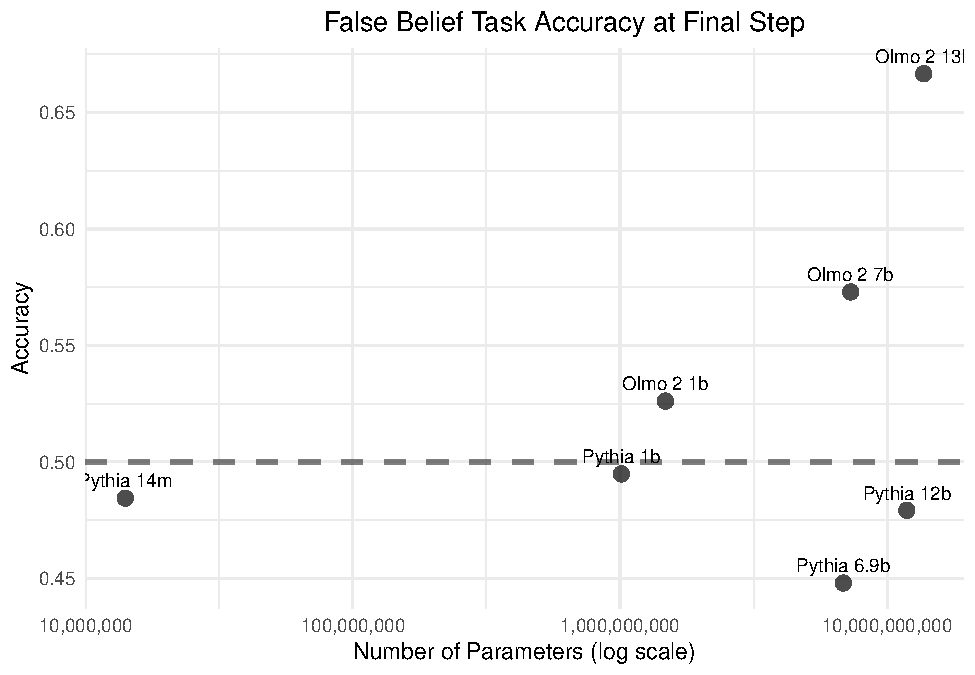
\includegraphics{fb_analysis_files/figure-latex/unnamed-chunk-3-1.pdf}

\begin{Shaded}
\begin{Highlighting}[]
\CommentTok{\# PAPER FIGURE: Plot displays fb task accuracy for all steps, final step in red}
\FunctionTok{ggplot}\NormalTok{(df\_summ, }\FunctionTok{aes}\NormalTok{(}\AttributeTok{x =}\NormalTok{ n\_params\_approx, }\AttributeTok{y =}\NormalTok{ mean\_accuracy)) }\SpecialCharTok{+}
  \FunctionTok{geom\_line}\NormalTok{(}\FunctionTok{aes}\NormalTok{(}\AttributeTok{group =}\NormalTok{ model\_shorthand), }\AttributeTok{alpha =} \FloatTok{0.3}\NormalTok{, }\AttributeTok{color =} \StringTok{"gray"}\NormalTok{) }\SpecialCharTok{+}
  \FunctionTok{geom\_point}\NormalTok{(}\AttributeTok{alpha =} \FloatTok{0.3}\NormalTok{, }\AttributeTok{size =} \DecValTok{1}\NormalTok{, }\AttributeTok{color =} \StringTok{"gray"}\NormalTok{) }\SpecialCharTok{+}
  \FunctionTok{geom\_point}\NormalTok{(}\AttributeTok{data =}\NormalTok{ final\_accuracy, }\AttributeTok{size =} \DecValTok{4}\NormalTok{, }
             \FunctionTok{aes}\NormalTok{(}\AttributeTok{color =}\NormalTok{ model\_family), }
             \AttributeTok{alpha =} \FloatTok{0.8}\NormalTok{) }\SpecialCharTok{+}
  \FunctionTok{geom\_hline}\NormalTok{(}\AttributeTok{yintercept =}\NormalTok{ .}\DecValTok{5}\NormalTok{, }\AttributeTok{linetype =} \StringTok{"dashed"}\NormalTok{,}
             \AttributeTok{size =} \FloatTok{1.2}\NormalTok{, }\AttributeTok{alpha =}\NormalTok{ .}\DecValTok{5}\NormalTok{) }\SpecialCharTok{+}
  \FunctionTok{scale\_color\_manual}\NormalTok{(}\AttributeTok{values =}\NormalTok{ viridisLite}\SpecialCharTok{::}\FunctionTok{viridis}\NormalTok{(}\DecValTok{2}\NormalTok{, }\AttributeTok{option =} \StringTok{"mako"}\NormalTok{, }
                                                  \AttributeTok{begin =} \FloatTok{0.8}\NormalTok{, }\AttributeTok{end =} \FloatTok{0.15}\NormalTok{)) }\SpecialCharTok{+} 
  \FunctionTok{geom\_text\_repel}\NormalTok{(}\AttributeTok{data =}\NormalTok{ final\_accuracy, }\FunctionTok{aes}\NormalTok{(}\AttributeTok{label =}\NormalTok{ model\_shorthand), }\AttributeTok{size =} \DecValTok{3}\NormalTok{) }\SpecialCharTok{+}
  \FunctionTok{scale\_x\_log10}\NormalTok{(}\AttributeTok{labels =}\NormalTok{ scales}\SpecialCharTok{::}\FunctionTok{comma\_format}\NormalTok{()) }\SpecialCharTok{+}
  \FunctionTok{labs}\NormalTok{(}
    \AttributeTok{title =} \StringTok{"False Belief Task Accuracy: Progression and Final Step"}\NormalTok{,}
    \AttributeTok{subtitle =} \StringTok{"Red points highlight accuracy at final pretraining step"}\NormalTok{,}
    \AttributeTok{x =} \StringTok{"Number of Parameters (log scale)"}\NormalTok{,}
    \AttributeTok{y =} \StringTok{"Accuracy"}
\NormalTok{  ) }\SpecialCharTok{+}
  \FunctionTok{theme\_minimal}\NormalTok{()}
\end{Highlighting}
\end{Shaded}

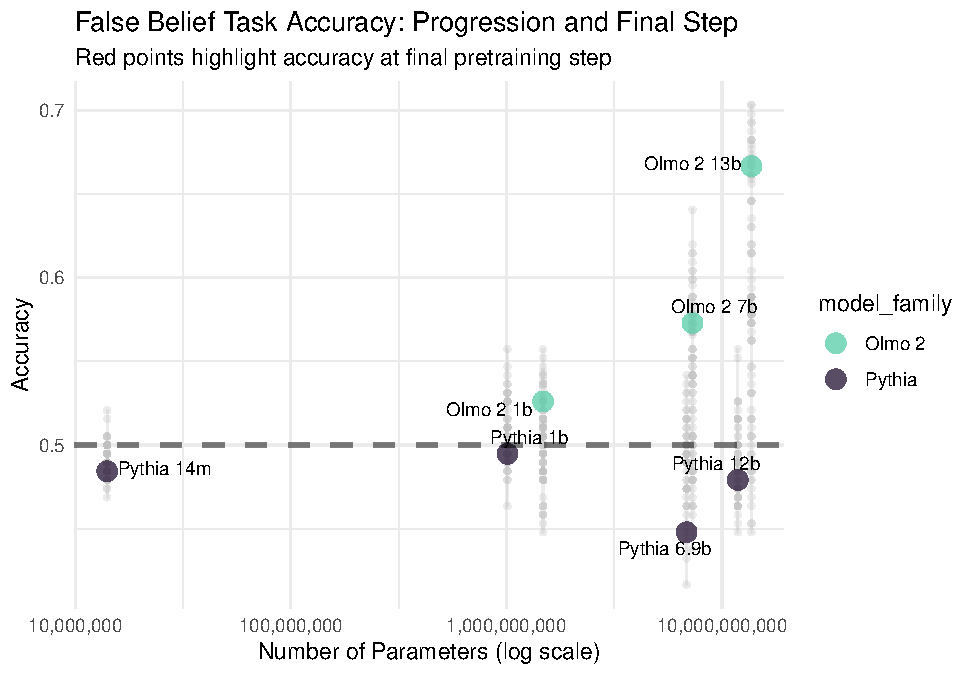
\includegraphics{fb_analysis_files/figure-latex/unnamed-chunk-3-2.pdf}

\begin{Shaded}
\begin{Highlighting}[]
\NormalTok{df\_summ }\SpecialCharTok{\%\textgreater{}\%}
  \FunctionTok{mutate}\NormalTok{(}\AttributeTok{step\_modded =}\NormalTok{ step }\SpecialCharTok{+} \DecValTok{1}\NormalTok{) }\SpecialCharTok{\%\textgreater{}\%}
  \FunctionTok{ggplot}\NormalTok{(}\FunctionTok{aes}\NormalTok{(}\AttributeTok{x =}\NormalTok{ step\_modded,}
             \AttributeTok{y =}\NormalTok{ mean\_accuracy,}
             \AttributeTok{color =}\NormalTok{ model\_shorthand)) }\SpecialCharTok{+}
  \CommentTok{\#geom\_point(size = 3,}
  \CommentTok{\#           alpha = .7) +}
  \FunctionTok{geom\_hline}\NormalTok{(}\AttributeTok{yintercept =}\NormalTok{ .}\DecValTok{83}\NormalTok{,}\DocumentationTok{\#\#TODO: Calculate from scratch}
             \AttributeTok{linetype =} \StringTok{"dotted"}\NormalTok{, }\AttributeTok{color =} \StringTok{"red"}\NormalTok{,}
             \AttributeTok{size =} \FloatTok{1.2}\NormalTok{, }\AttributeTok{alpha =}\NormalTok{ .}\DecValTok{8}\NormalTok{) }\SpecialCharTok{+} 
  \FunctionTok{geom\_line}\NormalTok{(}\AttributeTok{size =} \DecValTok{1}\NormalTok{) }\SpecialCharTok{+}
  \FunctionTok{geom\_hline}\NormalTok{(}\AttributeTok{yintercept =}\NormalTok{ .}\DecValTok{5}\NormalTok{, }\AttributeTok{linetype =} \StringTok{"dotted"}\NormalTok{,}
             \AttributeTok{size =} \FloatTok{1.2}\NormalTok{, }\AttributeTok{alpha =}\NormalTok{ .}\DecValTok{5}\NormalTok{) }\SpecialCharTok{+}
  \FunctionTok{scale\_x\_log10}\NormalTok{() }\SpecialCharTok{+}
  \CommentTok{\# geom\_text\_repel(aes(label=model\_shorthand), size=3) +}
  \FunctionTok{scale\_y\_continuous}\NormalTok{(}\AttributeTok{limits =} \FunctionTok{c}\NormalTok{(}\DecValTok{0}\NormalTok{, }\DecValTok{1}\NormalTok{)) }\SpecialCharTok{+}
  \FunctionTok{labs}\NormalTok{(}\AttributeTok{x =} \StringTok{"Step"}\NormalTok{,}
       \AttributeTok{y =} \StringTok{"Accuracy"}\NormalTok{,}
       \AttributeTok{color =} \StringTok{""}\NormalTok{,}
       \AttributeTok{shape =} \StringTok{""}\NormalTok{) }\SpecialCharTok{+}
  \FunctionTok{theme\_bw}\NormalTok{() }\SpecialCharTok{+}
  \FunctionTok{scale\_color\_manual}\NormalTok{(}\AttributeTok{values =}\NormalTok{ viridisLite}\SpecialCharTok{::}\FunctionTok{viridis}\NormalTok{(}\DecValTok{7}\NormalTok{, }\AttributeTok{option =} \StringTok{"mako"}\NormalTok{, }
                                                  \AttributeTok{begin =} \FloatTok{0.8}\NormalTok{, }\AttributeTok{end =} \FloatTok{0.15}\NormalTok{)) }\SpecialCharTok{+}
  \FunctionTok{theme}\NormalTok{(}\AttributeTok{text =} \FunctionTok{element\_text}\NormalTok{(}\AttributeTok{size =} \DecValTok{15}\NormalTok{),}
        \AttributeTok{legend.position=}\StringTok{"bottom"}\NormalTok{) }\SpecialCharTok{+}
  \FunctionTok{facet\_wrap}\NormalTok{(}\SpecialCharTok{\textasciitilde{}}\NormalTok{stage)}
\end{Highlighting}
\end{Shaded}

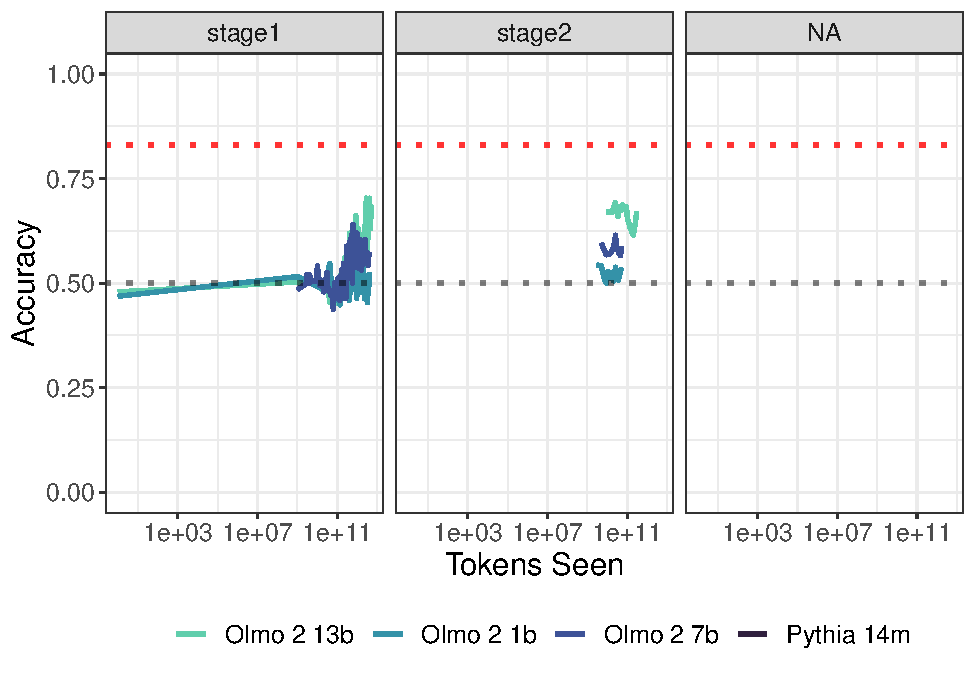
\includegraphics{fb_analysis_files/figure-latex/unnamed-chunk-3-3.pdf}

\begin{Shaded}
\begin{Highlighting}[]
\NormalTok{df\_summ }\SpecialCharTok{\%\textgreater{}\%}
  \FunctionTok{ggplot}\NormalTok{(}\FunctionTok{aes}\NormalTok{(}\AttributeTok{x =}\NormalTok{ tokens\_seen\_numeric\_mod,}
             \AttributeTok{y =}\NormalTok{ mean\_accuracy,}
             \AttributeTok{color =}\NormalTok{ model\_shorthand)) }\SpecialCharTok{+}
  \CommentTok{\#geom\_point(size = 3,}
    \CommentTok{\#         alpha = .7) +}
  \FunctionTok{geom\_line}\NormalTok{(}\AttributeTok{size =} \DecValTok{1}\NormalTok{, }\AttributeTok{alpha=}\FloatTok{0.7}\NormalTok{) }\SpecialCharTok{+}
  \FunctionTok{geom\_hline}\NormalTok{(}\AttributeTok{yintercept =}\NormalTok{ .}\DecValTok{5}\NormalTok{, }\AttributeTok{linetype =} \StringTok{"dashed"}\NormalTok{,}
             \AttributeTok{size =} \FloatTok{1.2}\NormalTok{, }\AttributeTok{alpha =}\NormalTok{ .}\DecValTok{5}\NormalTok{) }\SpecialCharTok{+}
  \FunctionTok{scale\_x\_log10}\NormalTok{(}\AttributeTok{labels =}\NormalTok{ scales}\SpecialCharTok{::}\FunctionTok{comma\_format}\NormalTok{()) }\SpecialCharTok{+}
  \CommentTok{\# geom\_text\_repel(aes(label=model\_shorthand), size=3) +}
  \FunctionTok{scale\_y\_continuous}\NormalTok{(}\AttributeTok{limits =} \FunctionTok{c}\NormalTok{(}\DecValTok{0}\NormalTok{, }\DecValTok{1}\NormalTok{)) }\SpecialCharTok{+}
  \FunctionTok{labs}\NormalTok{(}\AttributeTok{x =} \StringTok{"Tokens Seen"}\NormalTok{,}
       \AttributeTok{y =} \StringTok{"Accuracy"}\NormalTok{,}
       \AttributeTok{color =} \StringTok{""}\NormalTok{,}
       \AttributeTok{shape =} \StringTok{""}\NormalTok{) }\SpecialCharTok{+}
  \FunctionTok{theme\_bw}\NormalTok{() }\SpecialCharTok{+}
  \FunctionTok{scale\_color\_manual}\NormalTok{(}\AttributeTok{values =}\NormalTok{ viridisLite}\SpecialCharTok{::}\FunctionTok{viridis}\NormalTok{(}\DecValTok{7}\NormalTok{, }\AttributeTok{option =} \StringTok{"mako"}\NormalTok{, }
                                                  \AttributeTok{begin =} \FloatTok{0.9}\NormalTok{, }\AttributeTok{end =} \FloatTok{0.15}\NormalTok{)) }\SpecialCharTok{+}
  \FunctionTok{theme}\NormalTok{(}\AttributeTok{text =} \FunctionTok{element\_text}\NormalTok{(}\AttributeTok{size =} \DecValTok{15}\NormalTok{),}
        \AttributeTok{legend.position=}\StringTok{"bottom"}\NormalTok{) }\SpecialCharTok{+}
  \FunctionTok{facet\_wrap}\NormalTok{(}\SpecialCharTok{\textasciitilde{}}\NormalTok{stage)}
\end{Highlighting}
\end{Shaded}

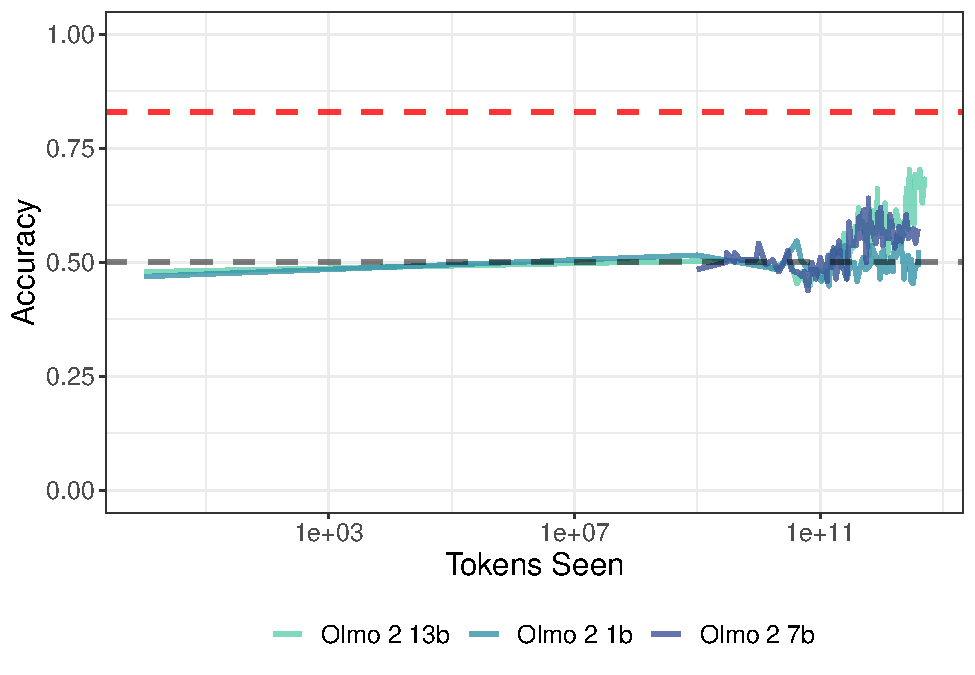
\includegraphics{fb_analysis_files/figure-latex/unnamed-chunk-3-4.pdf}

\begin{Shaded}
\begin{Highlighting}[]
\CommentTok{\# PAPER FIGURE: Plot of Olmo stage1 and Pythias}
\NormalTok{df\_summ }\SpecialCharTok{\%\textgreater{}\%}
  \FunctionTok{filter}\NormalTok{(stage }\SpecialCharTok{==} \StringTok{"stage1"} \SpecialCharTok{|} \FunctionTok{is.na}\NormalTok{(stage)) }\SpecialCharTok{\%\textgreater{}\%}
  \FunctionTok{ggplot}\NormalTok{(}\FunctionTok{aes}\NormalTok{(}\AttributeTok{x =}\NormalTok{ tokens\_seen\_numeric\_mod,}
             \AttributeTok{y =}\NormalTok{ mean\_accuracy,}
             \AttributeTok{color =}\NormalTok{ model\_shorthand)) }\SpecialCharTok{+}
  \FunctionTok{geom\_line}\NormalTok{(}\AttributeTok{size =} \FloatTok{1.5}\NormalTok{, }\AttributeTok{alpha =} \FloatTok{0.8}\NormalTok{) }\SpecialCharTok{+}
  \FunctionTok{geom\_hline}\NormalTok{(}\AttributeTok{yintercept =}\NormalTok{ .}\DecValTok{5}\NormalTok{, }\AttributeTok{linetype =} \StringTok{"dashed"}\NormalTok{,}
             \AttributeTok{size =} \FloatTok{1.2}\NormalTok{, }\AttributeTok{alpha =}\NormalTok{ .}\DecValTok{5}\NormalTok{) }\SpecialCharTok{+}
  \FunctionTok{scale\_x\_log10}\NormalTok{(}\AttributeTok{labels =}\NormalTok{ scales}\SpecialCharTok{::}\FunctionTok{comma\_format}\NormalTok{()) }\SpecialCharTok{+}
  \CommentTok{\# geom\_text\_repel(aes(label=model\_shorthand), size=3) +}
  \CommentTok{\#scale\_y\_continuous(limits = c(0.25, 0.75)) +}
  \FunctionTok{labs}\NormalTok{(}\AttributeTok{x =} \StringTok{"Tokens Seen"}\NormalTok{,}
       \AttributeTok{y =} \StringTok{"Accuracy"}\NormalTok{,}
       \AttributeTok{color =} \StringTok{""}\NormalTok{,}
       \AttributeTok{shape =} \StringTok{""}\NormalTok{) }\SpecialCharTok{+}
  \FunctionTok{theme\_bw}\NormalTok{() }\SpecialCharTok{+}
  \FunctionTok{scale\_color\_manual}\NormalTok{(}\AttributeTok{values =}\NormalTok{ viridisLite}\SpecialCharTok{::}\FunctionTok{viridis}\NormalTok{(}\DecValTok{7}\NormalTok{, }\AttributeTok{option =} \StringTok{"mako"}\NormalTok{, }
                                                  \AttributeTok{begin =} \FloatTok{0.8}\NormalTok{, }\AttributeTok{end =} \FloatTok{0.1}\NormalTok{)) }\SpecialCharTok{+}
  \FunctionTok{labs}\NormalTok{(}
    \AttributeTok{title =} \StringTok{"False Belief Task Accuracy Over Pretraining"}\NormalTok{,}
    \AttributeTok{x =} \StringTok{"Number of Tokens Seen (log scale)"}\NormalTok{,}
    \AttributeTok{y =} \StringTok{"Accuracy"}
\NormalTok{  ) }\SpecialCharTok{+}
  \FunctionTok{theme\_minimal}\NormalTok{() }\SpecialCharTok{+} 
  \FunctionTok{theme}\NormalTok{(}\AttributeTok{text =} \FunctionTok{element\_text}\NormalTok{(}\AttributeTok{size =} \DecValTok{15}\NormalTok{),}
        \AttributeTok{legend.position=}\StringTok{"bottom"}\NormalTok{) }
\end{Highlighting}
\end{Shaded}

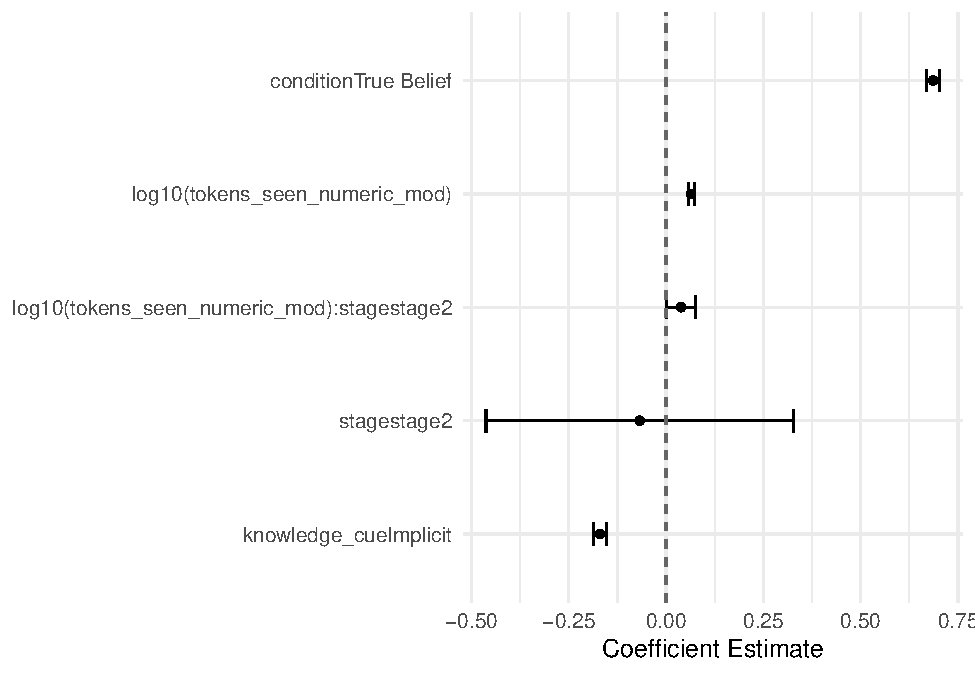
\includegraphics{fb_analysis_files/figure-latex/unnamed-chunk-3-5.pdf}

\begin{Shaded}
\begin{Highlighting}[]
\CommentTok{\# Filter for only stage1 olmo data and pythia models (e.g. exclude olmo stage2)}
\NormalTok{olmo\_and\_pythia }\OtherTok{\textless{}{-}}\NormalTok{ df\_all\_models\_fb }\SpecialCharTok{\%\textgreater{}\%}
  \FunctionTok{filter}\NormalTok{(stage }\SpecialCharTok{==} \StringTok{"stage1"} \SpecialCharTok{|} \FunctionTok{is.na}\NormalTok{(stage)) }
  
\DocumentationTok{\#\#\# PAPER LMER: How do model properties predict the probability of a correct response?}
\NormalTok{mod\_full }\OtherTok{=} \FunctionTok{glmer}\NormalTok{(}\AttributeTok{data =}\NormalTok{ olmo\_and\_pythia,}
\NormalTok{                 correct }\SpecialCharTok{\textasciitilde{}}\NormalTok{ condition }\SpecialCharTok{+}\NormalTok{ knowledge\_cue }\SpecialCharTok{+} 
                   \FunctionTok{log10}\NormalTok{(tokens\_seen\_numeric\_mod) }\SpecialCharTok{+}
\NormalTok{                   (}\DecValTok{1} \SpecialCharTok{|}\NormalTok{ start) }\SpecialCharTok{+}
\NormalTok{                   (}\DecValTok{1} \SpecialCharTok{|}\NormalTok{ model\_shorthand),}
                 \AttributeTok{family =} \FunctionTok{binomial}\NormalTok{())}
\FunctionTok{summary}\NormalTok{(mod\_full)}
\end{Highlighting}
\end{Shaded}

\begin{verbatim}
## Generalized linear mixed model fit by maximum likelihood (Laplace
##   Approximation) [glmerMod]
##  Family: binomial  ( logit )
## Formula: 
## correct ~ condition + knowledge_cue + log10(tokens_seen_numeric_mod) +  
##     (1 | start) + (1 | model_shorthand)
##    Data: olmo_and_pythia
## 
##      AIC      BIC   logLik deviance df.resid 
## 108729.2 108784.9 -54358.6 108717.2    80058 
## 
## Scaled residuals: 
##     Min      1Q  Median      3Q     Max 
## -1.5053 -0.9692  0.7153  0.9369  1.4325 
## 
## Random effects:
##  Groups          Name        Variance Std.Dev.
##  start           (Intercept) 0.011809 0.10867 
##  model_shorthand (Intercept) 0.009687 0.09842 
## Number of obs: 80064, groups:  start, 10; model_shorthand, 7
## 
## Fixed effects:
##                                 Estimate Std. Error z value Pr(>|z|)    
## (Intercept)                    -0.354592   0.069160  -5.127 2.94e-07 ***
## conditionTrue Belief            0.586821   0.014349  40.896  < 2e-16 ***
## knowledge_cueImplicit          -0.134477   0.014345  -9.374  < 2e-16 ***
## log10(tokens_seen_numeric_mod)  0.015500   0.004282   3.620 0.000294 ***
## ---
## Signif. codes:  0 '***' 0.001 '**' 0.01 '*' 0.05 '.' 0.1 ' ' 1
## 
## Correlation of Fixed Effects:
##             (Intr) cndtTB knwl_I
## condtnTrBlf -0.104              
## knwldg_cImp -0.102 -0.010       
## lg10(tk___) -0.656  0.004 -0.001
\end{verbatim}

\begin{Shaded}
\begin{Highlighting}[]
\DocumentationTok{\#\#\# Plot coefficients}
\NormalTok{df\_coef }\OtherTok{\textless{}{-}}\NormalTok{ broom.mixed}\SpecialCharTok{::}\FunctionTok{tidy}\NormalTok{(mod\_full, }\AttributeTok{effects =} \StringTok{"fixed"}\NormalTok{) }\SpecialCharTok{\%\textgreater{}\%}
  \FunctionTok{mutate}\NormalTok{(}\AttributeTok{term =}\NormalTok{ forcats}\SpecialCharTok{::}\FunctionTok{fct\_reorder}\NormalTok{(term, estimate))}


\NormalTok{df\_coef }\SpecialCharTok{\%\textgreater{}\%}
  \FunctionTok{filter}\NormalTok{(term }\SpecialCharTok{!=} \StringTok{"(Intercept)"}\NormalTok{) }\SpecialCharTok{\%\textgreater{}\%}
  \FunctionTok{ggplot}\NormalTok{(}\FunctionTok{aes}\NormalTok{(}\AttributeTok{x =}\NormalTok{ term, }\AttributeTok{y =}\NormalTok{ estimate)) }\SpecialCharTok{+}
  \FunctionTok{geom\_point}\NormalTok{() }\SpecialCharTok{+}
  \FunctionTok{geom\_errorbar}\NormalTok{(}\FunctionTok{aes}\NormalTok{(}\AttributeTok{ymin =}\NormalTok{ estimate }\SpecialCharTok{{-}}\NormalTok{ std.error, }\AttributeTok{ymax =}\NormalTok{ estimate }\SpecialCharTok{+}\NormalTok{ std.error),}
                \AttributeTok{width =} \FloatTok{0.2}\NormalTok{) }\SpecialCharTok{+}
  \FunctionTok{geom\_hline}\NormalTok{(}\AttributeTok{yintercept =} \DecValTok{0}\NormalTok{, }\AttributeTok{linetype =} \StringTok{"dashed"}\NormalTok{, }\AttributeTok{color =} \StringTok{"gray40"}\NormalTok{) }\SpecialCharTok{+}
  \FunctionTok{coord\_flip}\NormalTok{() }\SpecialCharTok{+}
  \FunctionTok{labs}\NormalTok{(}
    \AttributeTok{x =} \ConstantTok{NULL}\NormalTok{, }\AttributeTok{y =} \StringTok{"Coefficient Estimate"}\NormalTok{,}
\NormalTok{  ) }\SpecialCharTok{+}
  \FunctionTok{theme\_minimal}\NormalTok{(}\AttributeTok{base\_size =} \DecValTok{12}\NormalTok{)}
\end{Highlighting}
\end{Shaded}

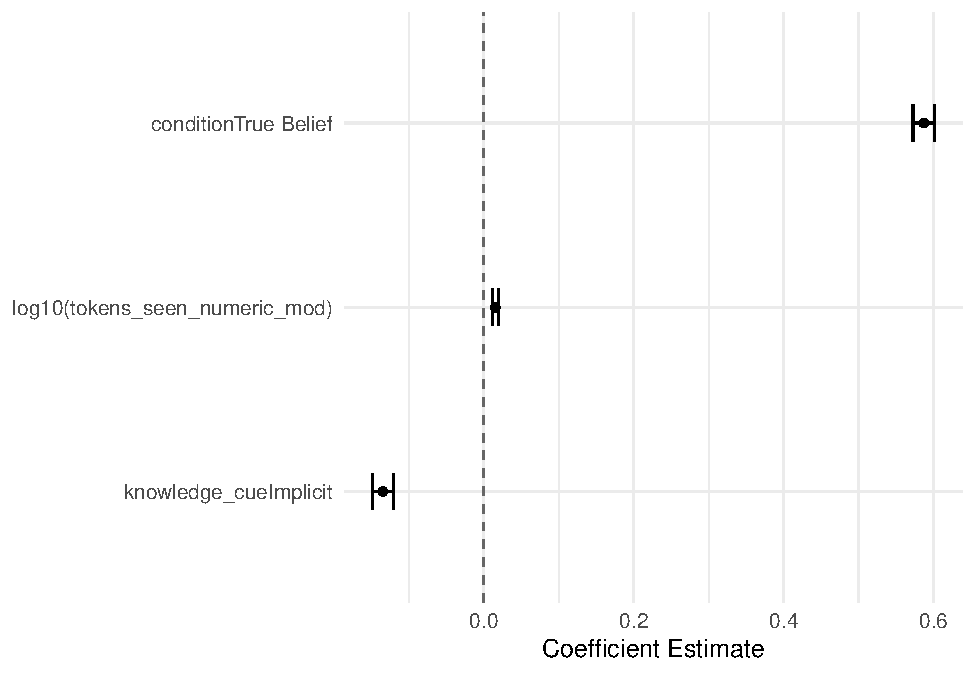
\includegraphics{fb_analysis_files/figure-latex/unnamed-chunk-3-6.pdf}

\begin{Shaded}
\begin{Highlighting}[]
\CommentTok{\# write.csv(df\_summ, "../../data/processed/summaries/fb\_summary.csv")}
\end{Highlighting}
\end{Shaded}

\hypertarget{phase-shift-modeling}{%
\subsection{Phase shift modeling}\label{phase-shift-modeling}}

Here, we predict the probability of a correct response over tokens seen,
focusing on stage 1.

\hypertarget{using-gam}{%
\subsubsection{Using GAM}\label{using-gam}}

\begin{Shaded}
\begin{Highlighting}[]
\FunctionTok{library}\NormalTok{(mgcv)}
\end{Highlighting}
\end{Shaded}

\begin{verbatim}
## Loading required package: nlme
\end{verbatim}

\begin{verbatim}
## 
## Attaching package: 'nlme'
\end{verbatim}

\begin{verbatim}
## The following object is masked from 'package:lme4':
## 
##     lmList
\end{verbatim}

\begin{verbatim}
## The following object is masked from 'package:dplyr':
## 
##     collapse
\end{verbatim}

\begin{verbatim}
## This is mgcv 1.8-42. For overview type 'help("mgcv-package")'.
\end{verbatim}

\begin{Shaded}
\begin{Highlighting}[]
\FunctionTok{library}\NormalTok{(dplyr)}
\FunctionTok{library}\NormalTok{(purrr)}

\CommentTok{\# Aggregate to get accuracy per checkpoint (helps GAM fit) for just Olmo stage1 \& pythia}
\NormalTok{df\_summary\_fb }\OtherTok{\textless{}{-}}\NormalTok{ olmo\_and\_pythia }\SpecialCharTok{\%\textgreater{}\%}
  \FunctionTok{filter}\NormalTok{(stage }\SpecialCharTok{==} \StringTok{"stage1"} \SpecialCharTok{|} \FunctionTok{is.na}\NormalTok{(stage)) }\SpecialCharTok{\%\textgreater{}\%}
  \FunctionTok{group\_by}\NormalTok{(model\_shorthand, }
\NormalTok{           condition, }
\NormalTok{           knowledge\_cue,}
\NormalTok{           step,}
\NormalTok{           tokens\_seen\_numeric\_mod) }\SpecialCharTok{\%\textgreater{}\%}
  \FunctionTok{summarise}\NormalTok{(}\AttributeTok{acc =} \FunctionTok{mean}\NormalTok{(correct), }\AttributeTok{.groups =} \StringTok{"drop"}\NormalTok{) }\SpecialCharTok{\%\textgreater{}\%}
  \FunctionTok{mutate}\NormalTok{(}\AttributeTok{log\_tokens =} \FunctionTok{log10}\NormalTok{(tokens\_seen\_numeric\_mod))}


\CommentTok{\# Fit a GAM for each model separately}
\NormalTok{fits }\OtherTok{\textless{}{-}}\NormalTok{ df\_summary\_fb }\SpecialCharTok{\%\textgreater{}\%}
  \FunctionTok{group\_split}\NormalTok{(model\_shorthand) }\SpecialCharTok{\%\textgreater{}\%}
  \FunctionTok{set\_names}\NormalTok{(}\FunctionTok{map\_chr}\NormalTok{(., }\SpecialCharTok{\textasciitilde{}} \FunctionTok{unique}\NormalTok{(.}\SpecialCharTok{$}\NormalTok{model\_shorthand))) }\SpecialCharTok{\%\textgreater{}\%}
  \FunctionTok{map}\NormalTok{(}\SpecialCharTok{\textasciitilde{}} \FunctionTok{gam}\NormalTok{(acc }\SpecialCharTok{\textasciitilde{}} \FunctionTok{s}\NormalTok{(tokens\_seen\_numeric\_mod, }\AttributeTok{k =} \DecValTok{10}\NormalTok{),}
            \AttributeTok{data =}\NormalTok{ ., }\AttributeTok{family =} \FunctionTok{binomial}\NormalTok{(}\AttributeTok{link =} \StringTok{"logit"}\NormalTok{)))  }\CommentTok{\# logistic is natural for accuracy}
\end{Highlighting}
\end{Shaded}

\begin{verbatim}
## Warning in eval(family$initialize): non-integer #successes in a binomial glm!

## Warning in eval(family$initialize): non-integer #successes in a binomial glm!

## Warning in eval(family$initialize): non-integer #successes in a binomial glm!

## Warning in eval(family$initialize): non-integer #successes in a binomial glm!

## Warning in eval(family$initialize): non-integer #successes in a binomial glm!

## Warning in eval(family$initialize): non-integer #successes in a binomial glm!

## Warning in eval(family$initialize): non-integer #successes in a binomial glm!

## Warning in eval(family$initialize): non-integer #successes in a binomial glm!

## Warning in eval(family$initialize): non-integer #successes in a binomial glm!

## Warning in eval(family$initialize): non-integer #successes in a binomial glm!

## Warning in eval(family$initialize): non-integer #successes in a binomial glm!

## Warning in eval(family$initialize): non-integer #successes in a binomial glm!

## Warning in eval(family$initialize): non-integer #successes in a binomial glm!

## Warning in eval(family$initialize): non-integer #successes in a binomial glm!

## Warning in eval(family$initialize): non-integer #successes in a binomial glm!

## Warning in eval(family$initialize): non-integer #successes in a binomial glm!

## Warning in eval(family$initialize): non-integer #successes in a binomial glm!

## Warning in eval(family$initialize): non-integer #successes in a binomial glm!

## Warning in eval(family$initialize): non-integer #successes in a binomial glm!

## Warning in eval(family$initialize): non-integer #successes in a binomial glm!

## Warning in eval(family$initialize): non-integer #successes in a binomial glm!

## Warning in eval(family$initialize): non-integer #successes in a binomial glm!

## Warning in eval(family$initialize): non-integer #successes in a binomial glm!

## Warning in eval(family$initialize): non-integer #successes in a binomial glm!

## Warning in eval(family$initialize): non-integer #successes in a binomial glm!

## Warning in eval(family$initialize): non-integer #successes in a binomial glm!

## Warning in eval(family$initialize): non-integer #successes in a binomial glm!

## Warning in eval(family$initialize): non-integer #successes in a binomial glm!

## Warning in eval(family$initialize): non-integer #successes in a binomial glm!

## Warning in eval(family$initialize): non-integer #successes in a binomial glm!

## Warning in eval(family$initialize): non-integer #successes in a binomial glm!

## Warning in eval(family$initialize): non-integer #successes in a binomial glm!

## Warning in eval(family$initialize): non-integer #successes in a binomial glm!

## Warning in eval(family$initialize): non-integer #successes in a binomial glm!

## Warning in eval(family$initialize): non-integer #successes in a binomial glm!

## Warning in eval(family$initialize): non-integer #successes in a binomial glm!

## Warning in eval(family$initialize): non-integer #successes in a binomial glm!

## Warning in eval(family$initialize): non-integer #successes in a binomial glm!

## Warning in eval(family$initialize): non-integer #successes in a binomial glm!

## Warning in eval(family$initialize): non-integer #successes in a binomial glm!

## Warning in eval(family$initialize): non-integer #successes in a binomial glm!

## Warning in eval(family$initialize): non-integer #successes in a binomial glm!

## Warning in eval(family$initialize): non-integer #successes in a binomial glm!

## Warning in eval(family$initialize): non-integer #successes in a binomial glm!

## Warning in eval(family$initialize): non-integer #successes in a binomial glm!

## Warning in eval(family$initialize): non-integer #successes in a binomial glm!

## Warning in eval(family$initialize): non-integer #successes in a binomial glm!

## Warning in eval(family$initialize): non-integer #successes in a binomial glm!

## Warning in eval(family$initialize): non-integer #successes in a binomial glm!

## Warning in eval(family$initialize): non-integer #successes in a binomial glm!

## Warning in eval(family$initialize): non-integer #successes in a binomial glm!

## Warning in eval(family$initialize): non-integer #successes in a binomial glm!

## Warning in eval(family$initialize): non-integer #successes in a binomial glm!

## Warning in eval(family$initialize): non-integer #successes in a binomial glm!

## Warning in eval(family$initialize): non-integer #successes in a binomial glm!

## Warning in eval(family$initialize): non-integer #successes in a binomial glm!

## Warning in eval(family$initialize): non-integer #successes in a binomial glm!

## Warning in eval(family$initialize): non-integer #successes in a binomial glm!

## Warning in eval(family$initialize): non-integer #successes in a binomial glm!

## Warning in eval(family$initialize): non-integer #successes in a binomial glm!

## Warning in eval(family$initialize): non-integer #successes in a binomial glm!

## Warning in eval(family$initialize): non-integer #successes in a binomial glm!

## Warning in eval(family$initialize): non-integer #successes in a binomial glm!

## Warning in eval(family$initialize): non-integer #successes in a binomial glm!

## Warning in eval(family$initialize): non-integer #successes in a binomial glm!

## Warning in eval(family$initialize): non-integer #successes in a binomial glm!

## Warning in eval(family$initialize): non-integer #successes in a binomial glm!

## Warning in eval(family$initialize): non-integer #successes in a binomial glm!

## Warning in eval(family$initialize): non-integer #successes in a binomial glm!

## Warning in eval(family$initialize): non-integer #successes in a binomial glm!

## Warning in eval(family$initialize): non-integer #successes in a binomial glm!

## Warning in eval(family$initialize): non-integer #successes in a binomial glm!

## Warning in eval(family$initialize): non-integer #successes in a binomial glm!

## Warning in eval(family$initialize): non-integer #successes in a binomial glm!

## Warning in eval(family$initialize): non-integer #successes in a binomial glm!

## Warning in eval(family$initialize): non-integer #successes in a binomial glm!

## Warning in eval(family$initialize): non-integer #successes in a binomial glm!

## Warning in eval(family$initialize): non-integer #successes in a binomial glm!

## Warning in eval(family$initialize): non-integer #successes in a binomial glm!

## Warning in eval(family$initialize): non-integer #successes in a binomial glm!

## Warning in eval(family$initialize): non-integer #successes in a binomial glm!

## Warning in eval(family$initialize): non-integer #successes in a binomial glm!

## Warning in eval(family$initialize): non-integer #successes in a binomial glm!

## Warning in eval(family$initialize): non-integer #successes in a binomial glm!
\end{verbatim}

\begin{Shaded}
\begin{Highlighting}[]
\NormalTok{df\_pred }\OtherTok{\textless{}{-}} \FunctionTok{map2\_df}\NormalTok{(fits, }\FunctionTok{names}\NormalTok{(fits), }\ControlFlowTok{function}\NormalTok{(mod, name) \{}
\NormalTok{  newdat }\OtherTok{\textless{}{-}} \FunctionTok{data.frame}\NormalTok{(}\AttributeTok{tokens\_seen\_numeric\_mod =} \FunctionTok{seq}\NormalTok{(}\FunctionTok{min}\NormalTok{(df\_summary\_fb}\SpecialCharTok{$}\NormalTok{tokens\_seen\_numeric\_mod),}
                                        \FunctionTok{max}\NormalTok{(df\_summary\_fb}\SpecialCharTok{$}\NormalTok{tokens\_seen\_numeric\_mod),}
                                        \AttributeTok{length.out =} \DecValTok{200}\NormalTok{))}
\NormalTok{  newdat}\SpecialCharTok{$}\NormalTok{acc\_hat }\OtherTok{\textless{}{-}} \FunctionTok{predict}\NormalTok{(mod, newdat, }\AttributeTok{type =} \StringTok{"response"}\NormalTok{)}
\NormalTok{  newdat}\SpecialCharTok{$}\NormalTok{model\_shorthand }\OtherTok{\textless{}{-}}\NormalTok{ name}
\NormalTok{  newdat}
\NormalTok{\})}

\CommentTok{\# PAPER FIGURE: plot of GAM fits for each model}
\FunctionTok{ggplot}\NormalTok{(df\_summary\_fb, }\FunctionTok{aes}\NormalTok{(}\AttributeTok{x =}\NormalTok{ tokens\_seen\_numeric\_mod, }\AttributeTok{y =}\NormalTok{ acc, }\AttributeTok{color =}\NormalTok{ model\_shorthand)) }\SpecialCharTok{+}
  \FunctionTok{geom\_point}\NormalTok{(}\AttributeTok{alpha =} \FloatTok{0.3}\NormalTok{) }\SpecialCharTok{+}
  \FunctionTok{geom\_line}\NormalTok{(}\AttributeTok{data =}\NormalTok{ df\_pred, }\FunctionTok{aes}\NormalTok{(}\AttributeTok{y =}\NormalTok{ acc\_hat), }\AttributeTok{size =} \FloatTok{1.2}\NormalTok{) }\SpecialCharTok{+}
  \FunctionTok{scale\_color\_manual}\NormalTok{(}\AttributeTok{values =}\NormalTok{ viridisLite}\SpecialCharTok{::}\FunctionTok{viridis}\NormalTok{(}\DecValTok{7}\NormalTok{, }\AttributeTok{option =} \StringTok{"mako"}\NormalTok{, }
                                                  \AttributeTok{begin =} \FloatTok{0.8}\NormalTok{, }\AttributeTok{end =} \FloatTok{0.15}\NormalTok{)) }\SpecialCharTok{+}
  \FunctionTok{scale\_x\_log10}\NormalTok{(}\AttributeTok{labels =}\NormalTok{ scales}\SpecialCharTok{::}\FunctionTok{comma\_format}\NormalTok{()) }\SpecialCharTok{+}
  \FunctionTok{labs}\NormalTok{(}
    \AttributeTok{title =} \StringTok{"Development of False Belief Task Performance"}\NormalTok{,}
    \AttributeTok{x =} \StringTok{"Number of Tokens Seen (log scale)"}\NormalTok{,}
    \AttributeTok{y =} \StringTok{"Accuracy"}
\NormalTok{  ) }\SpecialCharTok{+}
  \FunctionTok{theme\_minimal}\NormalTok{()}
\end{Highlighting}
\end{Shaded}

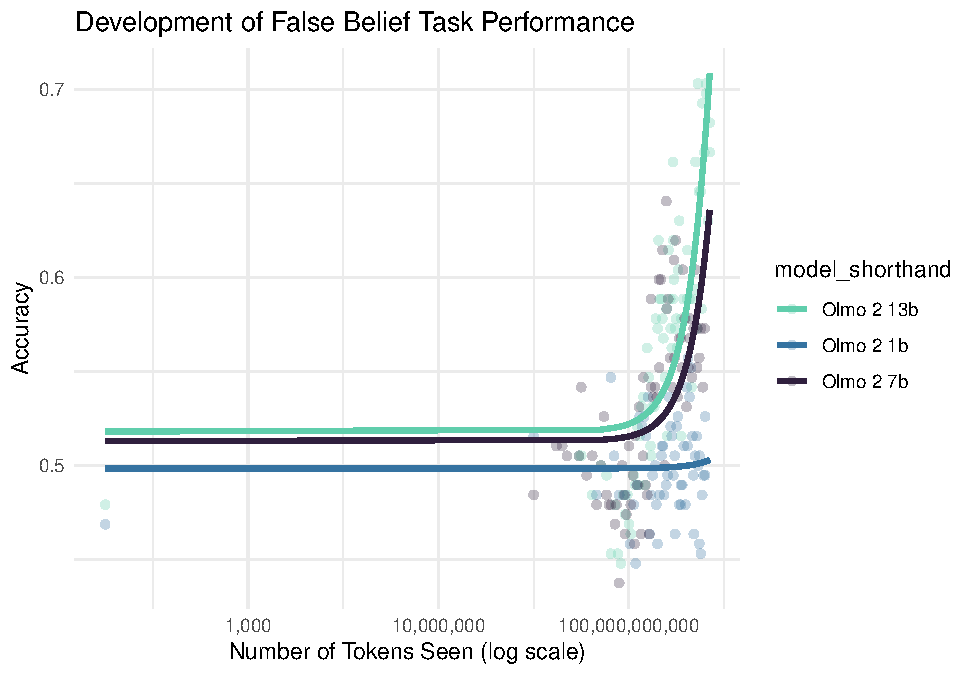
\includegraphics{fb_analysis_files/figure-latex/unnamed-chunk-4-1.pdf}

\begin{Shaded}
\begin{Highlighting}[]
\DocumentationTok{\#\#\# }\AlertTok{TODO}\DocumentationTok{: Identify inflection points}
\end{Highlighting}
\end{Shaded}

\hypertarget{situation-model-attention-check-results}{%
\section{Situation Model -- Attention Check
Results}\label{situation-model-attention-check-results}}

\textbf{TODO}: Unlike the original task, these aren't necessarily
balanced; so differences in probability of start vs.~end location, or
which person, could also affect accuracy. Could check on this too.

df\_tmp = df\_tmp \%\textgreater\% \# filter(stage == ``stage1'')
\%\textgreater\% mutate(model\_id = paste(stage, ``step'', ``-'', step))
\%\textgreater\% mutate(tokens\_seen\_numeric\_mod =
tokens\_seen\_numeric + 1)

\hypertarget{note-pythia-model-data-contains-a-main-checkpointstep-that-appears-as-a-nan-in-the-step-column}{%
\subsection{\texorpdfstring{NOTE: Pythia model data contains a ``main''
checkpoint/step that appears as a NaN in the \texttt{step}
column}{NOTE: Pythia model data contains a ``main'' checkpoint/step that appears as a NaN in the step column}}\label{note-pythia-model-data-contains-a-main-checkpointstep-that-appears-as-a-nan-in-the-step-column}}

\hypertarget{must-change-this-to-the-actual-value-of-the-final-step-143000}{%
\subsection{must change this to the actual value of the final step,
143000}\label{must-change-this-to-the-actual-value-of-the-final-step-143000}}

df\_tmp\(step[is.na(df_tmp\)step){]} \textless- 143000 \#hard-coded the
final step

\hypertarget{sort-df-columns-by-model-name-and-step-value}{%
\section{sort df columns by model name and step
value}\label{sort-df-columns-by-model-name-and-step-value}}

df\_tmp \textless- df\_tmp \%\textgreater\% arrange(model\_shorthand,
step) \# arrange in ascending order

metadata \textless- read\_csv(``../../data/raw/metadata\_models.csv'')
\# merge the metadata with the fb task df df\_all\_models\_fb \textless-
df\_tmp \%\textgreater\% left\_join(metadata, by = ``model\_shorthand'')

tokens\_seen\_pythia \textless-
read\_csv(``../../data/raw/pythia\_tokens\_seen.csv'') \# merge stepwise
tokens data for Pythia models df\_all\_models\_fb \textless-
df\_all\_models\_fb \%\textgreater\% left\_join(tokens\_seen\_pythia
\%\textgreater\% select(model\_shorthand, step, tokens\_seen\_from\_df1
= tokens\_seen\_numeric), by = c(``model\_shorthand'', ``step''))
\%\textgreater\% mutate(tokens\_seen\_numeric =
coalesce(tokens\_seen\_numeric, tokens\_seen\_from\_df1))
\%\textgreater\% select(-tokens\_seen\_from\_df1) \%\textgreater\%
mutate(tokens\_seen\_numeric\_mod = tokens\_seen\_numeric + 1)

df\_all\_models\_fb = df\_all\_models\_fb \%\textgreater\%
mutate(model\_family = case\_when( model\_shorthand \%in\% c(``Pythia
14m'', ``Pythia 1b'', ``Pythia 6.9b'', ``Pythia 12b'') \textasciitilde{}
``Pythia'', model\_shorthand \%in\% c(``Olmo 2 1b'', ``Olmo 2 7b'',
``Olmo 2 13b'') \textasciitilde{} ``Olmo 2'', ))

\begin{Shaded}
\begin{Highlighting}[]
\NormalTok{directory\_path }\OtherTok{\textless{}{-}} \StringTok{"../../data/processed/attn{-}checks{-}local/"}

\NormalTok{csv\_files }\OtherTok{\textless{}{-}} \FunctionTok{list.files}\NormalTok{(}\AttributeTok{path =}\NormalTok{ directory\_path, }\AttributeTok{pattern =} \StringTok{"*.csv"}\NormalTok{, }\AttributeTok{full.names =} \ConstantTok{TRUE}\NormalTok{)}
\NormalTok{csv\_list }\OtherTok{\textless{}{-}}\NormalTok{ csv\_files }\SpecialCharTok{\%\textgreater{}\%}
  \FunctionTok{map}\NormalTok{(}\SpecialCharTok{\textasciitilde{}} \FunctionTok{read\_csv}\NormalTok{(.))}
\end{Highlighting}
\end{Shaded}

\begin{verbatim}
## Rows: 768 Columns: 17
## -- Column specification --------------------------------------------------------
## Delimiter: ","
## chr (7): question, correct_answer, distractor_answer, model_path, model_shor...
## dbl (6): item, question_id, prob_correct, prob_distractor, log_odds, step
## lgl (4): item_id, condition, is_correct, ingredient
## 
## i Use `spec()` to retrieve the full column specification for this data.
## i Specify the column types or set `show_col_types = FALSE` to quiet this message.
## Rows: 768 Columns: 17
## -- Column specification --------------------------------------------------------
## Delimiter: ","
## chr (7): question, correct_answer, distractor_answer, model_path, model_shor...
## dbl (6): item, question_id, prob_correct, prob_distractor, log_odds, step
## lgl (4): item_id, condition, is_correct, ingredient
## 
## i Use `spec()` to retrieve the full column specification for this data.
## i Specify the column types or set `show_col_types = FALSE` to quiet this message.
## Rows: 768 Columns: 17
## -- Column specification --------------------------------------------------------
## Delimiter: ","
## chr (7): question, correct_answer, distractor_answer, model_path, model_shor...
## dbl (6): item, question_id, prob_correct, prob_distractor, log_odds, step
## lgl (4): item_id, condition, is_correct, ingredient
## 
## i Use `spec()` to retrieve the full column specification for this data.
## i Specify the column types or set `show_col_types = FALSE` to quiet this message.
## Rows: 768 Columns: 17
## -- Column specification --------------------------------------------------------
## Delimiter: ","
## chr (7): question, correct_answer, distractor_answer, model_path, model_shor...
## dbl (6): item, question_id, prob_correct, prob_distractor, log_odds, step
## lgl (4): item_id, condition, is_correct, ingredient
## 
## i Use `spec()` to retrieve the full column specification for this data.
## i Specify the column types or set `show_col_types = FALSE` to quiet this message.
## Rows: 768 Columns: 17
## -- Column specification --------------------------------------------------------
## Delimiter: ","
## chr (7): question, correct_answer, distractor_answer, model_path, model_shor...
## dbl (6): item, question_id, prob_correct, prob_distractor, log_odds, step
## lgl (4): item_id, condition, is_correct, ingredient
## 
## i Use `spec()` to retrieve the full column specification for this data.
## i Specify the column types or set `show_col_types = FALSE` to quiet this message.
## Rows: 768 Columns: 17
## -- Column specification --------------------------------------------------------
## Delimiter: ","
## chr (7): question, correct_answer, distractor_answer, model_path, model_shor...
## dbl (6): item, question_id, prob_correct, prob_distractor, log_odds, step
## lgl (4): item_id, condition, is_correct, ingredient
## 
## i Use `spec()` to retrieve the full column specification for this data.
## i Specify the column types or set `show_col_types = FALSE` to quiet this message.
## Rows: 768 Columns: 17
## -- Column specification --------------------------------------------------------
## Delimiter: ","
## chr (7): question, correct_answer, distractor_answer, model_path, model_shor...
## dbl (6): item, question_id, prob_correct, prob_distractor, log_odds, step
## lgl (4): item_id, condition, is_correct, ingredient
## 
## i Use `spec()` to retrieve the full column specification for this data.
## i Specify the column types or set `show_col_types = FALSE` to quiet this message.
## Rows: 768 Columns: 17
## -- Column specification --------------------------------------------------------
## Delimiter: ","
## chr (7): question, correct_answer, distractor_answer, model_path, model_shor...
## dbl (6): item, question_id, prob_correct, prob_distractor, log_odds, step
## lgl (4): item_id, condition, is_correct, ingredient
## 
## i Use `spec()` to retrieve the full column specification for this data.
## i Specify the column types or set `show_col_types = FALSE` to quiet this message.
## Rows: 768 Columns: 17
## -- Column specification --------------------------------------------------------
## Delimiter: ","
## chr (7): question, correct_answer, distractor_answer, model_path, model_shor...
## dbl (6): item, question_id, prob_correct, prob_distractor, log_odds, step
## lgl (4): item_id, condition, is_correct, ingredient
## 
## i Use `spec()` to retrieve the full column specification for this data.
## i Specify the column types or set `show_col_types = FALSE` to quiet this message.
## Rows: 768 Columns: 17
## -- Column specification --------------------------------------------------------
## Delimiter: ","
## chr (7): question, correct_answer, distractor_answer, model_path, model_shor...
## dbl (6): item, question_id, prob_correct, prob_distractor, log_odds, step
## lgl (4): item_id, condition, is_correct, ingredient
## 
## i Use `spec()` to retrieve the full column specification for this data.
## i Specify the column types or set `show_col_types = FALSE` to quiet this message.
## Rows: 768 Columns: 17
## -- Column specification --------------------------------------------------------
## Delimiter: ","
## chr (7): question, correct_answer, distractor_answer, model_path, model_shor...
## dbl (6): item, question_id, prob_correct, prob_distractor, log_odds, step
## lgl (4): item_id, condition, is_correct, ingredient
## 
## i Use `spec()` to retrieve the full column specification for this data.
## i Specify the column types or set `show_col_types = FALSE` to quiet this message.
## Rows: 768 Columns: 17
## -- Column specification --------------------------------------------------------
## Delimiter: ","
## chr (7): question, correct_answer, distractor_answer, model_path, model_shor...
## dbl (6): item, question_id, prob_correct, prob_distractor, log_odds, step
## lgl (4): item_id, condition, is_correct, ingredient
## 
## i Use `spec()` to retrieve the full column specification for this data.
## i Specify the column types or set `show_col_types = FALSE` to quiet this message.
## Rows: 768 Columns: 17
## -- Column specification --------------------------------------------------------
## Delimiter: ","
## chr (7): question, correct_answer, distractor_answer, model_path, model_shor...
## dbl (6): item, question_id, prob_correct, prob_distractor, log_odds, step
## lgl (4): item_id, condition, is_correct, ingredient
## 
## i Use `spec()` to retrieve the full column specification for this data.
## i Specify the column types or set `show_col_types = FALSE` to quiet this message.
## Rows: 768 Columns: 17
## -- Column specification --------------------------------------------------------
## Delimiter: ","
## chr (7): question, correct_answer, distractor_answer, model_path, model_shor...
## dbl (6): item, question_id, prob_correct, prob_distractor, log_odds, step
## lgl (4): item_id, condition, is_correct, ingredient
## 
## i Use `spec()` to retrieve the full column specification for this data.
## i Specify the column types or set `show_col_types = FALSE` to quiet this message.
## Rows: 768 Columns: 17
## -- Column specification --------------------------------------------------------
## Delimiter: ","
## chr (7): question, correct_answer, distractor_answer, model_path, model_shor...
## dbl (6): item, question_id, prob_correct, prob_distractor, log_odds, step
## lgl (4): item_id, condition, is_correct, ingredient
## 
## i Use `spec()` to retrieve the full column specification for this data.
## i Specify the column types or set `show_col_types = FALSE` to quiet this message.
## Rows: 768 Columns: 17
## -- Column specification --------------------------------------------------------
## Delimiter: ","
## chr (7): question, correct_answer, distractor_answer, model_path, model_shor...
## dbl (6): item, question_id, prob_correct, prob_distractor, log_odds, step
## lgl (4): item_id, condition, is_correct, ingredient
## 
## i Use `spec()` to retrieve the full column specification for this data.
## i Specify the column types or set `show_col_types = FALSE` to quiet this message.
## Rows: 768 Columns: 17
## -- Column specification --------------------------------------------------------
## Delimiter: ","
## chr (7): question, correct_answer, distractor_answer, model_path, model_shor...
## dbl (6): item, question_id, prob_correct, prob_distractor, log_odds, step
## lgl (4): item_id, condition, is_correct, ingredient
## 
## i Use `spec()` to retrieve the full column specification for this data.
## i Specify the column types or set `show_col_types = FALSE` to quiet this message.
## Rows: 768 Columns: 17
## -- Column specification --------------------------------------------------------
## Delimiter: ","
## chr (7): question, correct_answer, distractor_answer, model_path, model_shor...
## dbl (6): item, question_id, prob_correct, prob_distractor, log_odds, step
## lgl (4): item_id, condition, is_correct, ingredient
## 
## i Use `spec()` to retrieve the full column specification for this data.
## i Specify the column types or set `show_col_types = FALSE` to quiet this message.
## Rows: 768 Columns: 17
## -- Column specification --------------------------------------------------------
## Delimiter: ","
## chr (7): question, correct_answer, distractor_answer, model_path, model_shor...
## dbl (6): item, question_id, prob_correct, prob_distractor, log_odds, step
## lgl (4): item_id, condition, is_correct, ingredient
## 
## i Use `spec()` to retrieve the full column specification for this data.
## i Specify the column types or set `show_col_types = FALSE` to quiet this message.
## Rows: 768 Columns: 17
## -- Column specification --------------------------------------------------------
## Delimiter: ","
## chr (7): question, correct_answer, distractor_answer, model_path, model_shor...
## dbl (6): item, question_id, prob_correct, prob_distractor, log_odds, step
## lgl (4): item_id, condition, is_correct, ingredient
## 
## i Use `spec()` to retrieve the full column specification for this data.
## i Specify the column types or set `show_col_types = FALSE` to quiet this message.
## Rows: 768 Columns: 17
## -- Column specification --------------------------------------------------------
## Delimiter: ","
## chr (7): question, correct_answer, distractor_answer, model_path, model_shor...
## dbl (6): item, question_id, prob_correct, prob_distractor, log_odds, step
## lgl (4): item_id, condition, is_correct, ingredient
## 
## i Use `spec()` to retrieve the full column specification for this data.
## i Specify the column types or set `show_col_types = FALSE` to quiet this message.
## Rows: 768 Columns: 17
## -- Column specification --------------------------------------------------------
## Delimiter: ","
## chr (7): question, correct_answer, distractor_answer, model_path, model_shor...
## dbl (6): item, question_id, prob_correct, prob_distractor, log_odds, step
## lgl (4): item_id, condition, is_correct, ingredient
## 
## i Use `spec()` to retrieve the full column specification for this data.
## i Specify the column types or set `show_col_types = FALSE` to quiet this message.
## Rows: 768 Columns: 17
## -- Column specification --------------------------------------------------------
## Delimiter: ","
## chr (7): question, correct_answer, distractor_answer, model_path, model_shor...
## dbl (6): item, question_id, prob_correct, prob_distractor, log_odds, step
## lgl (4): item_id, condition, is_correct, ingredient
## 
## i Use `spec()` to retrieve the full column specification for this data.
## i Specify the column types or set `show_col_types = FALSE` to quiet this message.
## Rows: 768 Columns: 17
## -- Column specification --------------------------------------------------------
## Delimiter: ","
## chr (7): question, correct_answer, distractor_answer, model_path, model_shor...
## dbl (6): item, question_id, prob_correct, prob_distractor, log_odds, step
## lgl (4): item_id, condition, is_correct, ingredient
## 
## i Use `spec()` to retrieve the full column specification for this data.
## i Specify the column types or set `show_col_types = FALSE` to quiet this message.
## Rows: 768 Columns: 17
## -- Column specification --------------------------------------------------------
## Delimiter: ","
## chr (7): question, correct_answer, distractor_answer, model_path, model_shor...
## dbl (6): item, question_id, prob_correct, prob_distractor, log_odds, step
## lgl (4): item_id, condition, is_correct, ingredient
## 
## i Use `spec()` to retrieve the full column specification for this data.
## i Specify the column types or set `show_col_types = FALSE` to quiet this message.
## Rows: 768 Columns: 17
## -- Column specification --------------------------------------------------------
## Delimiter: ","
## chr (7): question, correct_answer, distractor_answer, model_path, model_shor...
## dbl (6): item, question_id, prob_correct, prob_distractor, log_odds, step
## lgl (4): item_id, condition, is_correct, ingredient
## 
## i Use `spec()` to retrieve the full column specification for this data.
## i Specify the column types or set `show_col_types = FALSE` to quiet this message.
## Rows: 768 Columns: 17
## -- Column specification --------------------------------------------------------
## Delimiter: ","
## chr (7): question, correct_answer, distractor_answer, model_path, model_shor...
## dbl (6): item, question_id, prob_correct, prob_distractor, log_odds, step
## lgl (4): item_id, condition, is_correct, ingredient
## 
## i Use `spec()` to retrieve the full column specification for this data.
## i Specify the column types or set `show_col_types = FALSE` to quiet this message.
## Rows: 768 Columns: 17
## -- Column specification --------------------------------------------------------
## Delimiter: ","
## chr (7): question, correct_answer, distractor_answer, model_path, model_shor...
## dbl (6): item, question_id, prob_correct, prob_distractor, log_odds, step
## lgl (4): item_id, condition, is_correct, ingredient
## 
## i Use `spec()` to retrieve the full column specification for this data.
## i Specify the column types or set `show_col_types = FALSE` to quiet this message.
## Rows: 768 Columns: 17
## -- Column specification --------------------------------------------------------
## Delimiter: ","
## chr (7): question, correct_answer, distractor_answer, model_path, model_shor...
## dbl (6): item, question_id, prob_correct, prob_distractor, log_odds, step
## lgl (4): item_id, condition, is_correct, ingredient
## 
## i Use `spec()` to retrieve the full column specification for this data.
## i Specify the column types or set `show_col_types = FALSE` to quiet this message.
## Rows: 768 Columns: 17
## -- Column specification --------------------------------------------------------
## Delimiter: ","
## chr (7): question, correct_answer, distractor_answer, model_path, model_shor...
## dbl (6): item, question_id, prob_correct, prob_distractor, log_odds, step
## lgl (4): item_id, condition, is_correct, ingredient
## 
## i Use `spec()` to retrieve the full column specification for this data.
## i Specify the column types or set `show_col_types = FALSE` to quiet this message.
## Rows: 768 Columns: 17
## -- Column specification --------------------------------------------------------
## Delimiter: ","
## chr (7): question, correct_answer, distractor_answer, model_path, model_shor...
## dbl (6): item, question_id, prob_correct, prob_distractor, log_odds, step
## lgl (4): item_id, condition, is_correct, ingredient
## 
## i Use `spec()` to retrieve the full column specification for this data.
## i Specify the column types or set `show_col_types = FALSE` to quiet this message.
## Rows: 768 Columns: 17
## -- Column specification --------------------------------------------------------
## Delimiter: ","
## chr (7): question, correct_answer, distractor_answer, model_path, model_shor...
## dbl (6): item, question_id, prob_correct, prob_distractor, log_odds, step
## lgl (4): item_id, condition, is_correct, ingredient
## 
## i Use `spec()` to retrieve the full column specification for this data.
## i Specify the column types or set `show_col_types = FALSE` to quiet this message.
## Rows: 768 Columns: 17
## -- Column specification --------------------------------------------------------
## Delimiter: ","
## chr (7): question, correct_answer, distractor_answer, model_path, model_shor...
## dbl (6): item, question_id, prob_correct, prob_distractor, log_odds, step
## lgl (4): item_id, condition, is_correct, ingredient
## 
## i Use `spec()` to retrieve the full column specification for this data.
## i Specify the column types or set `show_col_types = FALSE` to quiet this message.
## Rows: 768 Columns: 17
## -- Column specification --------------------------------------------------------
## Delimiter: ","
## chr (7): question, correct_answer, distractor_answer, model_path, model_shor...
## dbl (6): item, question_id, prob_correct, prob_distractor, log_odds, step
## lgl (4): item_id, condition, is_correct, ingredient
## 
## i Use `spec()` to retrieve the full column specification for this data.
## i Specify the column types or set `show_col_types = FALSE` to quiet this message.
## Rows: 768 Columns: 17
## -- Column specification --------------------------------------------------------
## Delimiter: ","
## chr (7): question, correct_answer, distractor_answer, model_path, model_shor...
## dbl (6): item, question_id, prob_correct, prob_distractor, log_odds, step
## lgl (4): item_id, condition, is_correct, ingredient
## 
## i Use `spec()` to retrieve the full column specification for this data.
## i Specify the column types or set `show_col_types = FALSE` to quiet this message.
## Rows: 768 Columns: 17
## -- Column specification --------------------------------------------------------
## Delimiter: ","
## chr (7): question, correct_answer, distractor_answer, model_path, model_shor...
## dbl (6): item, question_id, prob_correct, prob_distractor, log_odds, step
## lgl (4): item_id, condition, is_correct, ingredient
## 
## i Use `spec()` to retrieve the full column specification for this data.
## i Specify the column types or set `show_col_types = FALSE` to quiet this message.
## Rows: 768 Columns: 17
## -- Column specification --------------------------------------------------------
## Delimiter: ","
## chr (7): question, correct_answer, distractor_answer, model_path, model_shor...
## dbl (6): item, question_id, prob_correct, prob_distractor, log_odds, step
## lgl (4): item_id, condition, is_correct, ingredient
## 
## i Use `spec()` to retrieve the full column specification for this data.
## i Specify the column types or set `show_col_types = FALSE` to quiet this message.
## Rows: 768 Columns: 17
## -- Column specification --------------------------------------------------------
## Delimiter: ","
## chr (7): question, correct_answer, distractor_answer, model_path, model_shor...
## dbl (6): item, question_id, prob_correct, prob_distractor, log_odds, step
## lgl (4): item_id, condition, is_correct, ingredient
## 
## i Use `spec()` to retrieve the full column specification for this data.
## i Specify the column types or set `show_col_types = FALSE` to quiet this message.
## Rows: 768 Columns: 17
## -- Column specification --------------------------------------------------------
## Delimiter: ","
## chr (7): question, correct_answer, distractor_answer, model_path, model_shor...
## dbl (6): item, question_id, prob_correct, prob_distractor, log_odds, step
## lgl (4): item_id, condition, is_correct, ingredient
## 
## i Use `spec()` to retrieve the full column specification for this data.
## i Specify the column types or set `show_col_types = FALSE` to quiet this message.
## Rows: 768 Columns: 17
## -- Column specification --------------------------------------------------------
## Delimiter: ","
## chr (7): question, correct_answer, distractor_answer, model_path, model_shor...
## dbl (6): item, question_id, prob_correct, prob_distractor, log_odds, step
## lgl (4): item_id, condition, is_correct, ingredient
## 
## i Use `spec()` to retrieve the full column specification for this data.
## i Specify the column types or set `show_col_types = FALSE` to quiet this message.
## Rows: 768 Columns: 17
## -- Column specification --------------------------------------------------------
## Delimiter: ","
## chr (7): question, correct_answer, distractor_answer, model_path, model_shor...
## dbl (6): item, question_id, prob_correct, prob_distractor, log_odds, step
## lgl (4): item_id, condition, is_correct, ingredient
## 
## i Use `spec()` to retrieve the full column specification for this data.
## i Specify the column types or set `show_col_types = FALSE` to quiet this message.
## Rows: 768 Columns: 17
## -- Column specification --------------------------------------------------------
## Delimiter: ","
## chr (7): question, correct_answer, distractor_answer, model_path, model_shor...
## dbl (6): item, question_id, prob_correct, prob_distractor, log_odds, step
## lgl (4): item_id, condition, is_correct, ingredient
## 
## i Use `spec()` to retrieve the full column specification for this data.
## i Specify the column types or set `show_col_types = FALSE` to quiet this message.
## Rows: 768 Columns: 17
## -- Column specification --------------------------------------------------------
## Delimiter: ","
## chr (7): question, correct_answer, distractor_answer, model_path, model_shor...
## dbl (6): item, question_id, prob_correct, prob_distractor, log_odds, step
## lgl (4): item_id, condition, is_correct, ingredient
## 
## i Use `spec()` to retrieve the full column specification for this data.
## i Specify the column types or set `show_col_types = FALSE` to quiet this message.
## Rows: 768 Columns: 17
## -- Column specification --------------------------------------------------------
## Delimiter: ","
## chr (7): question, correct_answer, distractor_answer, model_path, model_shor...
## dbl (6): item, question_id, prob_correct, prob_distractor, log_odds, step
## lgl (4): item_id, condition, is_correct, ingredient
## 
## i Use `spec()` to retrieve the full column specification for this data.
## i Specify the column types or set `show_col_types = FALSE` to quiet this message.
## Rows: 768 Columns: 17
## -- Column specification --------------------------------------------------------
## Delimiter: ","
## chr (7): question, correct_answer, distractor_answer, model_path, model_shor...
## dbl (6): item, question_id, prob_correct, prob_distractor, log_odds, step
## lgl (4): item_id, condition, is_correct, ingredient
## 
## i Use `spec()` to retrieve the full column specification for this data.
## i Specify the column types or set `show_col_types = FALSE` to quiet this message.
## Rows: 768 Columns: 17
## -- Column specification --------------------------------------------------------
## Delimiter: ","
## chr (7): question, correct_answer, distractor_answer, model_path, model_shor...
## dbl (6): item, question_id, prob_correct, prob_distractor, log_odds, step
## lgl (4): item_id, condition, is_correct, ingredient
## 
## i Use `spec()` to retrieve the full column specification for this data.
## i Specify the column types or set `show_col_types = FALSE` to quiet this message.
## Rows: 768 Columns: 17
## -- Column specification --------------------------------------------------------
## Delimiter: ","
## chr (7): question, correct_answer, distractor_answer, model_path, model_shor...
## dbl (6): item, question_id, prob_correct, prob_distractor, log_odds, step
## lgl (4): item_id, condition, is_correct, ingredient
## 
## i Use `spec()` to retrieve the full column specification for this data.
## i Specify the column types or set `show_col_types = FALSE` to quiet this message.
## Rows: 768 Columns: 17
## -- Column specification --------------------------------------------------------
## Delimiter: ","
## chr (7): question, correct_answer, distractor_answer, model_path, model_shor...
## dbl (6): item, question_id, prob_correct, prob_distractor, log_odds, step
## lgl (4): item_id, condition, is_correct, ingredient
## 
## i Use `spec()` to retrieve the full column specification for this data.
## i Specify the column types or set `show_col_types = FALSE` to quiet this message.
## Rows: 768 Columns: 17
## -- Column specification --------------------------------------------------------
## Delimiter: ","
## chr (7): question, correct_answer, distractor_answer, model_path, model_shor...
## dbl (6): item, question_id, prob_correct, prob_distractor, log_odds, step
## lgl (4): item_id, condition, is_correct, ingredient
## 
## i Use `spec()` to retrieve the full column specification for this data.
## i Specify the column types or set `show_col_types = FALSE` to quiet this message.
## Rows: 768 Columns: 17
## -- Column specification --------------------------------------------------------
## Delimiter: ","
## chr (7): question, correct_answer, distractor_answer, model_path, model_shor...
## dbl (6): item, question_id, prob_correct, prob_distractor, log_odds, step
## lgl (4): item_id, condition, is_correct, ingredient
## 
## i Use `spec()` to retrieve the full column specification for this data.
## i Specify the column types or set `show_col_types = FALSE` to quiet this message.
## Rows: 768 Columns: 17
## -- Column specification --------------------------------------------------------
## Delimiter: ","
## chr (7): question, correct_answer, distractor_answer, model_path, model_shor...
## dbl (6): item, question_id, prob_correct, prob_distractor, log_odds, step
## lgl (4): item_id, condition, is_correct, ingredient
## 
## i Use `spec()` to retrieve the full column specification for this data.
## i Specify the column types or set `show_col_types = FALSE` to quiet this message.
## Rows: 768 Columns: 17
## -- Column specification --------------------------------------------------------
## Delimiter: ","
## chr (7): question, correct_answer, distractor_answer, model_path, model_shor...
## dbl (6): item, question_id, prob_correct, prob_distractor, log_odds, step
## lgl (4): item_id, condition, is_correct, ingredient
## 
## i Use `spec()` to retrieve the full column specification for this data.
## i Specify the column types or set `show_col_types = FALSE` to quiet this message.
## Rows: 768 Columns: 17
## -- Column specification --------------------------------------------------------
## Delimiter: ","
## chr (7): question, correct_answer, distractor_answer, model_path, model_shor...
## dbl (6): item, question_id, prob_correct, prob_distractor, log_odds, step
## lgl (4): item_id, condition, is_correct, ingredient
## 
## i Use `spec()` to retrieve the full column specification for this data.
## i Specify the column types or set `show_col_types = FALSE` to quiet this message.
## Rows: 768 Columns: 17
## -- Column specification --------------------------------------------------------
## Delimiter: ","
## chr (7): question, correct_answer, distractor_answer, model_path, model_shor...
## dbl (6): item, question_id, prob_correct, prob_distractor, log_odds, step
## lgl (4): item_id, condition, is_correct, ingredient
## 
## i Use `spec()` to retrieve the full column specification for this data.
## i Specify the column types or set `show_col_types = FALSE` to quiet this message.
## Rows: 768 Columns: 17
## -- Column specification --------------------------------------------------------
## Delimiter: ","
## chr (7): question, correct_answer, distractor_answer, model_path, model_shor...
## dbl (6): item, question_id, prob_correct, prob_distractor, log_odds, step
## lgl (4): item_id, condition, is_correct, ingredient
## 
## i Use `spec()` to retrieve the full column specification for this data.
## i Specify the column types or set `show_col_types = FALSE` to quiet this message.
## Rows: 768 Columns: 17
## -- Column specification --------------------------------------------------------
## Delimiter: ","
## chr (8): question, correct_answer, distractor_answer, model_path, model_shor...
## dbl (6): item, question_id, prob_correct, prob_distractor, log_odds, step
## lgl (3): item_id, condition, is_correct
## 
## i Use `spec()` to retrieve the full column specification for this data.
## i Specify the column types or set `show_col_types = FALSE` to quiet this message.
## Rows: 768 Columns: 17
## -- Column specification --------------------------------------------------------
## Delimiter: ","
## chr (8): question, correct_answer, distractor_answer, model_path, model_shor...
## dbl (6): item, question_id, prob_correct, prob_distractor, log_odds, step
## lgl (3): item_id, condition, is_correct
## 
## i Use `spec()` to retrieve the full column specification for this data.
## i Specify the column types or set `show_col_types = FALSE` to quiet this message.
## Rows: 768 Columns: 17
## -- Column specification --------------------------------------------------------
## Delimiter: ","
## chr (8): question, correct_answer, distractor_answer, model_path, model_shor...
## dbl (6): item, question_id, prob_correct, prob_distractor, log_odds, step
## lgl (3): item_id, condition, is_correct
## 
## i Use `spec()` to retrieve the full column specification for this data.
## i Specify the column types or set `show_col_types = FALSE` to quiet this message.
## Rows: 768 Columns: 17
## -- Column specification --------------------------------------------------------
## Delimiter: ","
## chr (8): question, correct_answer, distractor_answer, model_path, model_shor...
## dbl (6): item, question_id, prob_correct, prob_distractor, log_odds, step
## lgl (3): item_id, condition, is_correct
## 
## i Use `spec()` to retrieve the full column specification for this data.
## i Specify the column types or set `show_col_types = FALSE` to quiet this message.
## Rows: 768 Columns: 17
## -- Column specification --------------------------------------------------------
## Delimiter: ","
## chr (8): question, correct_answer, distractor_answer, model_path, model_shor...
## dbl (6): item, question_id, prob_correct, prob_distractor, log_odds, step
## lgl (3): item_id, condition, is_correct
## 
## i Use `spec()` to retrieve the full column specification for this data.
## i Specify the column types or set `show_col_types = FALSE` to quiet this message.
## Rows: 768 Columns: 17
## -- Column specification --------------------------------------------------------
## Delimiter: ","
## chr (8): question, correct_answer, distractor_answer, model_path, model_shor...
## dbl (6): item, question_id, prob_correct, prob_distractor, log_odds, step
## lgl (3): item_id, condition, is_correct
## 
## i Use `spec()` to retrieve the full column specification for this data.
## i Specify the column types or set `show_col_types = FALSE` to quiet this message.
## Rows: 768 Columns: 17
## -- Column specification --------------------------------------------------------
## Delimiter: ","
## chr (8): question, correct_answer, distractor_answer, model_path, model_shor...
## dbl (6): item, question_id, prob_correct, prob_distractor, log_odds, step
## lgl (3): item_id, condition, is_correct
## 
## i Use `spec()` to retrieve the full column specification for this data.
## i Specify the column types or set `show_col_types = FALSE` to quiet this message.
## Rows: 768 Columns: 17
## -- Column specification --------------------------------------------------------
## Delimiter: ","
## chr (8): question, correct_answer, distractor_answer, model_path, model_shor...
## dbl (6): item, question_id, prob_correct, prob_distractor, log_odds, step
## lgl (3): item_id, condition, is_correct
## 
## i Use `spec()` to retrieve the full column specification for this data.
## i Specify the column types or set `show_col_types = FALSE` to quiet this message.
## Rows: 768 Columns: 17
## -- Column specification --------------------------------------------------------
## Delimiter: ","
## chr (8): question, correct_answer, distractor_answer, model_path, model_shor...
## dbl (6): item, question_id, prob_correct, prob_distractor, log_odds, step
## lgl (3): item_id, condition, is_correct
## 
## i Use `spec()` to retrieve the full column specification for this data.
## i Specify the column types or set `show_col_types = FALSE` to quiet this message.
## Rows: 768 Columns: 17
## -- Column specification --------------------------------------------------------
## Delimiter: ","
## chr (8): question, correct_answer, distractor_answer, model_path, model_shor...
## dbl (6): item, question_id, prob_correct, prob_distractor, log_odds, step
## lgl (3): item_id, condition, is_correct
## 
## i Use `spec()` to retrieve the full column specification for this data.
## i Specify the column types or set `show_col_types = FALSE` to quiet this message.
## Rows: 768 Columns: 17
## -- Column specification --------------------------------------------------------
## Delimiter: ","
## chr (8): question, correct_answer, distractor_answer, model_path, model_shor...
## dbl (6): item, question_id, prob_correct, prob_distractor, log_odds, step
## lgl (3): item_id, condition, is_correct
## 
## i Use `spec()` to retrieve the full column specification for this data.
## i Specify the column types or set `show_col_types = FALSE` to quiet this message.
## Rows: 768 Columns: 17
## -- Column specification --------------------------------------------------------
## Delimiter: ","
## chr (8): question, correct_answer, distractor_answer, model_path, model_shor...
## dbl (6): item, question_id, prob_correct, prob_distractor, log_odds, step
## lgl (3): item_id, condition, is_correct
## 
## i Use `spec()` to retrieve the full column specification for this data.
## i Specify the column types or set `show_col_types = FALSE` to quiet this message.
## Rows: 768 Columns: 17
## -- Column specification --------------------------------------------------------
## Delimiter: ","
## chr (8): question, correct_answer, distractor_answer, model_path, model_shor...
## dbl (6): item, question_id, prob_correct, prob_distractor, log_odds, step
## lgl (3): item_id, condition, is_correct
## 
## i Use `spec()` to retrieve the full column specification for this data.
## i Specify the column types or set `show_col_types = FALSE` to quiet this message.
## Rows: 768 Columns: 17
## -- Column specification --------------------------------------------------------
## Delimiter: ","
## chr (8): question, correct_answer, distractor_answer, model_path, model_shor...
## dbl (6): item, question_id, prob_correct, prob_distractor, log_odds, step
## lgl (3): item_id, condition, is_correct
## 
## i Use `spec()` to retrieve the full column specification for this data.
## i Specify the column types or set `show_col_types = FALSE` to quiet this message.
## Rows: 768 Columns: 17
## -- Column specification --------------------------------------------------------
## Delimiter: ","
## chr (8): question, correct_answer, distractor_answer, model_path, model_shor...
## dbl (6): item, question_id, prob_correct, prob_distractor, log_odds, step
## lgl (3): item_id, condition, is_correct
## 
## i Use `spec()` to retrieve the full column specification for this data.
## i Specify the column types or set `show_col_types = FALSE` to quiet this message.
## Rows: 768 Columns: 17
## -- Column specification --------------------------------------------------------
## Delimiter: ","
## chr (8): question, correct_answer, distractor_answer, model_path, model_shor...
## dbl (6): item, question_id, prob_correct, prob_distractor, log_odds, step
## lgl (3): item_id, condition, is_correct
## 
## i Use `spec()` to retrieve the full column specification for this data.
## i Specify the column types or set `show_col_types = FALSE` to quiet this message.
## Rows: 768 Columns: 17
## -- Column specification --------------------------------------------------------
## Delimiter: ","
## chr (8): question, correct_answer, distractor_answer, model_path, model_shor...
## dbl (6): item, question_id, prob_correct, prob_distractor, log_odds, step
## lgl (3): item_id, condition, is_correct
## 
## i Use `spec()` to retrieve the full column specification for this data.
## i Specify the column types or set `show_col_types = FALSE` to quiet this message.
## Rows: 768 Columns: 17
## -- Column specification --------------------------------------------------------
## Delimiter: ","
## chr (8): question, correct_answer, distractor_answer, model_path, model_shor...
## dbl (6): item, question_id, prob_correct, prob_distractor, log_odds, step
## lgl (3): item_id, condition, is_correct
## 
## i Use `spec()` to retrieve the full column specification for this data.
## i Specify the column types or set `show_col_types = FALSE` to quiet this message.
## Rows: 768 Columns: 17
## -- Column specification --------------------------------------------------------
## Delimiter: ","
## chr (8): question, correct_answer, distractor_answer, model_path, model_shor...
## dbl (6): item, question_id, prob_correct, prob_distractor, log_odds, step
## lgl (3): item_id, condition, is_correct
## 
## i Use `spec()` to retrieve the full column specification for this data.
## i Specify the column types or set `show_col_types = FALSE` to quiet this message.
## Rows: 768 Columns: 17
## -- Column specification --------------------------------------------------------
## Delimiter: ","
## chr (8): question, correct_answer, distractor_answer, model_path, model_shor...
## dbl (6): item, question_id, prob_correct, prob_distractor, log_odds, step
## lgl (3): item_id, condition, is_correct
## 
## i Use `spec()` to retrieve the full column specification for this data.
## i Specify the column types or set `show_col_types = FALSE` to quiet this message.
## Rows: 768 Columns: 17
## -- Column specification --------------------------------------------------------
## Delimiter: ","
## chr (8): question, correct_answer, distractor_answer, model_path, model_shor...
## dbl (6): item, question_id, prob_correct, prob_distractor, log_odds, step
## lgl (3): item_id, condition, is_correct
## 
## i Use `spec()` to retrieve the full column specification for this data.
## i Specify the column types or set `show_col_types = FALSE` to quiet this message.
## Rows: 768 Columns: 17
## -- Column specification --------------------------------------------------------
## Delimiter: ","
## chr (8): question, correct_answer, distractor_answer, model_path, model_shor...
## dbl (6): item, question_id, prob_correct, prob_distractor, log_odds, step
## lgl (3): item_id, condition, is_correct
## 
## i Use `spec()` to retrieve the full column specification for this data.
## i Specify the column types or set `show_col_types = FALSE` to quiet this message.
## Rows: 768 Columns: 17
## -- Column specification --------------------------------------------------------
## Delimiter: ","
## chr (8): question, correct_answer, distractor_answer, model_path, model_shor...
## dbl (6): item, question_id, prob_correct, prob_distractor, log_odds, step
## lgl (3): item_id, condition, is_correct
## 
## i Use `spec()` to retrieve the full column specification for this data.
## i Specify the column types or set `show_col_types = FALSE` to quiet this message.
## Rows: 768 Columns: 17
## -- Column specification --------------------------------------------------------
## Delimiter: ","
## chr (8): question, correct_answer, distractor_answer, model_path, model_shor...
## dbl (6): item, question_id, prob_correct, prob_distractor, log_odds, step
## lgl (3): item_id, condition, is_correct
## 
## i Use `spec()` to retrieve the full column specification for this data.
## i Specify the column types or set `show_col_types = FALSE` to quiet this message.
## Rows: 768 Columns: 17
## -- Column specification --------------------------------------------------------
## Delimiter: ","
## chr (8): question, correct_answer, distractor_answer, model_path, model_shor...
## dbl (6): item, question_id, prob_correct, prob_distractor, log_odds, step
## lgl (3): item_id, condition, is_correct
## 
## i Use `spec()` to retrieve the full column specification for this data.
## i Specify the column types or set `show_col_types = FALSE` to quiet this message.
## Rows: 768 Columns: 17
## -- Column specification --------------------------------------------------------
## Delimiter: ","
## chr (8): question, correct_answer, distractor_answer, model_path, model_shor...
## dbl (6): item, question_id, prob_correct, prob_distractor, log_odds, step
## lgl (3): item_id, condition, is_correct
## 
## i Use `spec()` to retrieve the full column specification for this data.
## i Specify the column types or set `show_col_types = FALSE` to quiet this message.
## Rows: 768 Columns: 17
## -- Column specification --------------------------------------------------------
## Delimiter: ","
## chr (8): question, correct_answer, distractor_answer, model_path, model_shor...
## dbl (6): item, question_id, prob_correct, prob_distractor, log_odds, step
## lgl (3): item_id, condition, is_correct
## 
## i Use `spec()` to retrieve the full column specification for this data.
## i Specify the column types or set `show_col_types = FALSE` to quiet this message.
## Rows: 768 Columns: 17
## -- Column specification --------------------------------------------------------
## Delimiter: ","
## chr (8): question, correct_answer, distractor_answer, model_path, model_shor...
## dbl (6): item, question_id, prob_correct, prob_distractor, log_odds, step
## lgl (3): item_id, condition, is_correct
## 
## i Use `spec()` to retrieve the full column specification for this data.
## i Specify the column types or set `show_col_types = FALSE` to quiet this message.
## Rows: 768 Columns: 17
## -- Column specification --------------------------------------------------------
## Delimiter: ","
## chr (8): question, correct_answer, distractor_answer, model_path, model_shor...
## dbl (6): item, question_id, prob_correct, prob_distractor, log_odds, step
## lgl (3): item_id, condition, is_correct
## 
## i Use `spec()` to retrieve the full column specification for this data.
## i Specify the column types or set `show_col_types = FALSE` to quiet this message.
## Rows: 768 Columns: 17
## -- Column specification --------------------------------------------------------
## Delimiter: ","
## chr (8): question, correct_answer, distractor_answer, model_path, model_shor...
## dbl (6): item, question_id, prob_correct, prob_distractor, log_odds, step
## lgl (3): item_id, condition, is_correct
## 
## i Use `spec()` to retrieve the full column specification for this data.
## i Specify the column types or set `show_col_types = FALSE` to quiet this message.
## Rows: 768 Columns: 17
## -- Column specification --------------------------------------------------------
## Delimiter: ","
## chr (8): question, correct_answer, distractor_answer, model_path, model_shor...
## dbl (6): item, question_id, prob_correct, prob_distractor, log_odds, step
## lgl (3): item_id, condition, is_correct
## 
## i Use `spec()` to retrieve the full column specification for this data.
## i Specify the column types or set `show_col_types = FALSE` to quiet this message.
## Rows: 768 Columns: 17
## -- Column specification --------------------------------------------------------
## Delimiter: ","
## chr (8): question, correct_answer, distractor_answer, model_path, model_shor...
## dbl (6): item, question_id, prob_correct, prob_distractor, log_odds, step
## lgl (3): item_id, condition, is_correct
## 
## i Use `spec()` to retrieve the full column specification for this data.
## i Specify the column types or set `show_col_types = FALSE` to quiet this message.
## Rows: 768 Columns: 17
## -- Column specification --------------------------------------------------------
## Delimiter: ","
## chr (8): question, correct_answer, distractor_answer, model_path, model_shor...
## dbl (6): item, question_id, prob_correct, prob_distractor, log_odds, step
## lgl (3): item_id, condition, is_correct
## 
## i Use `spec()` to retrieve the full column specification for this data.
## i Specify the column types or set `show_col_types = FALSE` to quiet this message.
## Rows: 768 Columns: 17
## -- Column specification --------------------------------------------------------
## Delimiter: ","
## chr (7): question, correct_answer, distractor_answer, model_path, model_shor...
## dbl (6): item, question_id, prob_correct, prob_distractor, log_odds, step
## lgl (4): item_id, condition, is_correct, ingredient
## 
## i Use `spec()` to retrieve the full column specification for this data.
## i Specify the column types or set `show_col_types = FALSE` to quiet this message.
## Rows: 768 Columns: 17
## -- Column specification --------------------------------------------------------
## Delimiter: ","
## chr (7): question, correct_answer, distractor_answer, model_path, model_shor...
## dbl (6): item, question_id, prob_correct, prob_distractor, log_odds, step
## lgl (4): item_id, condition, is_correct, ingredient
## 
## i Use `spec()` to retrieve the full column specification for this data.
## i Specify the column types or set `show_col_types = FALSE` to quiet this message.
## Rows: 768 Columns: 17
## -- Column specification --------------------------------------------------------
## Delimiter: ","
## chr (7): question, correct_answer, distractor_answer, model_path, model_shor...
## dbl (6): item, question_id, prob_correct, prob_distractor, log_odds, step
## lgl (4): item_id, condition, is_correct, ingredient
## 
## i Use `spec()` to retrieve the full column specification for this data.
## i Specify the column types or set `show_col_types = FALSE` to quiet this message.
## Rows: 768 Columns: 13
## -- Column specification --------------------------------------------------------
## Delimiter: ","
## chr (5): question, correct_answer, distractor_answer, model_path, model_shor...
## dbl (5): item, question_id, prob_correct, prob_distractor, log_odds
## lgl (3): item_id, condition, is_correct
## 
## i Use `spec()` to retrieve the full column specification for this data.
## i Specify the column types or set `show_col_types = FALSE` to quiet this message.
## Rows: 768 Columns: 17
## -- Column specification --------------------------------------------------------
## Delimiter: ","
## chr (7): question, correct_answer, distractor_answer, model_path, model_shor...
## dbl (6): item, question_id, prob_correct, prob_distractor, log_odds, step
## lgl (4): item_id, condition, is_correct, ingredient
## 
## i Use `spec()` to retrieve the full column specification for this data.
## i Specify the column types or set `show_col_types = FALSE` to quiet this message.
## Rows: 768 Columns: 17
## -- Column specification --------------------------------------------------------
## Delimiter: ","
## chr (7): question, correct_answer, distractor_answer, model_path, model_shor...
## dbl (6): item, question_id, prob_correct, prob_distractor, log_odds, step
## lgl (4): item_id, condition, is_correct, ingredient
## 
## i Use `spec()` to retrieve the full column specification for this data.
## i Specify the column types or set `show_col_types = FALSE` to quiet this message.
## Rows: 768 Columns: 13
## -- Column specification --------------------------------------------------------
## Delimiter: ","
## chr (5): question, correct_answer, distractor_answer, model_path, model_shor...
## dbl (5): item, question_id, prob_correct, prob_distractor, log_odds
## lgl (3): item_id, condition, is_correct
## 
## i Use `spec()` to retrieve the full column specification for this data.
## i Specify the column types or set `show_col_types = FALSE` to quiet this message.
## Rows: 768 Columns: 17
## -- Column specification --------------------------------------------------------
## Delimiter: ","
## chr (7): question, correct_answer, distractor_answer, model_path, model_shor...
## dbl (6): item, question_id, prob_correct, prob_distractor, log_odds, step
## lgl (4): item_id, condition, is_correct, ingredient
## 
## i Use `spec()` to retrieve the full column specification for this data.
## i Specify the column types or set `show_col_types = FALSE` to quiet this message.
## Rows: 768 Columns: 17
## -- Column specification --------------------------------------------------------
## Delimiter: ","
## chr (7): question, correct_answer, distractor_answer, model_path, model_shor...
## dbl (6): item, question_id, prob_correct, prob_distractor, log_odds, step
## lgl (4): item_id, condition, is_correct, ingredient
## 
## i Use `spec()` to retrieve the full column specification for this data.
## i Specify the column types or set `show_col_types = FALSE` to quiet this message.
## Rows: 768 Columns: 17
## -- Column specification --------------------------------------------------------
## Delimiter: ","
## chr (7): question, correct_answer, distractor_answer, model_path, model_shor...
## dbl (6): item, question_id, prob_correct, prob_distractor, log_odds, step
## lgl (4): item_id, condition, is_correct, ingredient
## 
## i Use `spec()` to retrieve the full column specification for this data.
## i Specify the column types or set `show_col_types = FALSE` to quiet this message.
## Rows: 768 Columns: 17
## -- Column specification --------------------------------------------------------
## Delimiter: ","
## chr (7): question, correct_answer, distractor_answer, model_path, model_shor...
## dbl (6): item, question_id, prob_correct, prob_distractor, log_odds, step
## lgl (4): item_id, condition, is_correct, ingredient
## 
## i Use `spec()` to retrieve the full column specification for this data.
## i Specify the column types or set `show_col_types = FALSE` to quiet this message.
## Rows: 768 Columns: 17
## -- Column specification --------------------------------------------------------
## Delimiter: ","
## chr (7): question, correct_answer, distractor_answer, model_path, model_shor...
## dbl (6): item, question_id, prob_correct, prob_distractor, log_odds, step
## lgl (4): item_id, condition, is_correct, ingredient
## 
## i Use `spec()` to retrieve the full column specification for this data.
## i Specify the column types or set `show_col_types = FALSE` to quiet this message.
## Rows: 768 Columns: 13
## -- Column specification --------------------------------------------------------
## Delimiter: ","
## chr (5): question, correct_answer, distractor_answer, model_path, model_shor...
## dbl (5): item, question_id, prob_correct, prob_distractor, log_odds
## lgl (3): item_id, condition, is_correct
## 
## i Use `spec()` to retrieve the full column specification for this data.
## i Specify the column types or set `show_col_types = FALSE` to quiet this message.
## Rows: 768 Columns: 17
## -- Column specification --------------------------------------------------------
## Delimiter: ","
## chr (7): question, correct_answer, distractor_answer, model_path, model_shor...
## dbl (6): item, question_id, prob_correct, prob_distractor, log_odds, step
## lgl (4): item_id, condition, is_correct, ingredient
## 
## i Use `spec()` to retrieve the full column specification for this data.
## i Specify the column types or set `show_col_types = FALSE` to quiet this message.
## Rows: 768 Columns: 17
## -- Column specification --------------------------------------------------------
## Delimiter: ","
## chr (7): question, correct_answer, distractor_answer, model_path, model_shor...
## dbl (6): item, question_id, prob_correct, prob_distractor, log_odds, step
## lgl (4): item_id, condition, is_correct, ingredient
## 
## i Use `spec()` to retrieve the full column specification for this data.
## i Specify the column types or set `show_col_types = FALSE` to quiet this message.
## Rows: 768 Columns: 17
## -- Column specification --------------------------------------------------------
## Delimiter: ","
## chr (7): question, correct_answer, distractor_answer, model_path, model_shor...
## dbl (6): item, question_id, prob_correct, prob_distractor, log_odds, step
## lgl (4): item_id, condition, is_correct, ingredient
## 
## i Use `spec()` to retrieve the full column specification for this data.
## i Specify the column types or set `show_col_types = FALSE` to quiet this message.
## Rows: 768 Columns: 13
## -- Column specification --------------------------------------------------------
## Delimiter: ","
## chr (5): question, correct_answer, distractor_answer, model_path, model_shor...
## dbl (5): item, question_id, prob_correct, prob_distractor, log_odds
## lgl (3): item_id, condition, is_correct
## 
## i Use `spec()` to retrieve the full column specification for this data.
## i Specify the column types or set `show_col_types = FALSE` to quiet this message.
## Rows: 768 Columns: 17
## -- Column specification --------------------------------------------------------
## Delimiter: ","
## chr (7): question, correct_answer, distractor_answer, model_path, model_shor...
## dbl (6): item, question_id, prob_correct, prob_distractor, log_odds, step
## lgl (4): item_id, condition, is_correct, ingredient
## 
## i Use `spec()` to retrieve the full column specification for this data.
## i Specify the column types or set `show_col_types = FALSE` to quiet this message.
## Rows: 768 Columns: 17
## -- Column specification --------------------------------------------------------
## Delimiter: ","
## chr (7): question, correct_answer, distractor_answer, model_path, model_shor...
## dbl (6): item, question_id, prob_correct, prob_distractor, log_odds, step
## lgl (4): item_id, condition, is_correct, ingredient
## 
## i Use `spec()` to retrieve the full column specification for this data.
## i Specify the column types or set `show_col_types = FALSE` to quiet this message.
## Rows: 768 Columns: 17
## -- Column specification --------------------------------------------------------
## Delimiter: ","
## chr (7): question, correct_answer, distractor_answer, model_path, model_shor...
## dbl (6): item, question_id, prob_correct, prob_distractor, log_odds, step
## lgl (4): item_id, condition, is_correct, ingredient
## 
## i Use `spec()` to retrieve the full column specification for this data.
## i Specify the column types or set `show_col_types = FALSE` to quiet this message.
## Rows: 768 Columns: 17
## -- Column specification --------------------------------------------------------
## Delimiter: ","
## chr (7): question, correct_answer, distractor_answer, model_path, model_shor...
## dbl (6): item, question_id, prob_correct, prob_distractor, log_odds, step
## lgl (4): item_id, condition, is_correct, ingredient
## 
## i Use `spec()` to retrieve the full column specification for this data.
## i Specify the column types or set `show_col_types = FALSE` to quiet this message.
## Rows: 768 Columns: 13
## -- Column specification --------------------------------------------------------
## Delimiter: ","
## chr (5): question, correct_answer, distractor_answer, model_path, model_shor...
## dbl (5): item, question_id, prob_correct, prob_distractor, log_odds
## lgl (3): item_id, condition, is_correct
## 
## i Use `spec()` to retrieve the full column specification for this data.
## i Specify the column types or set `show_col_types = FALSE` to quiet this message.
## Rows: 768 Columns: 17
## -- Column specification --------------------------------------------------------
## Delimiter: ","
## chr (7): question, correct_answer, distractor_answer, model_path, model_shor...
## dbl (6): item, question_id, prob_correct, prob_distractor, log_odds, step
## lgl (4): item_id, condition, is_correct, ingredient
## 
## i Use `spec()` to retrieve the full column specification for this data.
## i Specify the column types or set `show_col_types = FALSE` to quiet this message.
## Rows: 768 Columns: 17
## -- Column specification --------------------------------------------------------
## Delimiter: ","
## chr (7): question, correct_answer, distractor_answer, model_path, model_shor...
## dbl (6): item, question_id, prob_correct, prob_distractor, log_odds, step
## lgl (4): item_id, condition, is_correct, ingredient
## 
## i Use `spec()` to retrieve the full column specification for this data.
## i Specify the column types or set `show_col_types = FALSE` to quiet this message.
## Rows: 768 Columns: 17
## -- Column specification --------------------------------------------------------
## Delimiter: ","
## chr (7): question, correct_answer, distractor_answer, model_path, model_shor...
## dbl (6): item, question_id, prob_correct, prob_distractor, log_odds, step
## lgl (4): item_id, condition, is_correct, ingredient
## 
## i Use `spec()` to retrieve the full column specification for this data.
## i Specify the column types or set `show_col_types = FALSE` to quiet this message.
## Rows: 768 Columns: 17
## -- Column specification --------------------------------------------------------
## Delimiter: ","
## chr (7): question, correct_answer, distractor_answer, model_path, model_shor...
## dbl (6): item, question_id, prob_correct, prob_distractor, log_odds, step
## lgl (4): item_id, condition, is_correct, ingredient
## 
## i Use `spec()` to retrieve the full column specification for this data.
## i Specify the column types or set `show_col_types = FALSE` to quiet this message.
## Rows: 768 Columns: 17
## -- Column specification --------------------------------------------------------
## Delimiter: ","
## chr (7): question, correct_answer, distractor_answer, model_path, model_shor...
## dbl (6): item, question_id, prob_correct, prob_distractor, log_odds, step
## lgl (4): item_id, condition, is_correct, ingredient
## 
## i Use `spec()` to retrieve the full column specification for this data.
## i Specify the column types or set `show_col_types = FALSE` to quiet this message.
## Rows: 768 Columns: 17
## -- Column specification --------------------------------------------------------
## Delimiter: ","
## chr (7): question, correct_answer, distractor_answer, model_path, model_shor...
## dbl (6): item, question_id, prob_correct, prob_distractor, log_odds, step
## lgl (4): item_id, condition, is_correct, ingredient
## 
## i Use `spec()` to retrieve the full column specification for this data.
## i Specify the column types or set `show_col_types = FALSE` to quiet this message.
## Rows: 768 Columns: 13
## -- Column specification --------------------------------------------------------
## Delimiter: ","
## chr (5): question, correct_answer, distractor_answer, model_path, model_shor...
## dbl (5): item, question_id, prob_correct, prob_distractor, log_odds
## lgl (3): item_id, condition, is_correct
## 
## i Use `spec()` to retrieve the full column specification for this data.
## i Specify the column types or set `show_col_types = FALSE` to quiet this message.
## Rows: 768 Columns: 17
## -- Column specification --------------------------------------------------------
## Delimiter: ","
## chr (7): question, correct_answer, distractor_answer, model_path, model_shor...
## dbl (6): item, question_id, prob_correct, prob_distractor, log_odds, step
## lgl (4): item_id, condition, is_correct, ingredient
## 
## i Use `spec()` to retrieve the full column specification for this data.
## i Specify the column types or set `show_col_types = FALSE` to quiet this message.
## Rows: 768 Columns: 13
## -- Column specification --------------------------------------------------------
## Delimiter: ","
## chr (5): question, correct_answer, distractor_answer, model_path, model_shor...
## dbl (5): item, question_id, prob_correct, prob_distractor, log_odds
## lgl (3): item_id, condition, is_correct
## 
## i Use `spec()` to retrieve the full column specification for this data.
## i Specify the column types or set `show_col_types = FALSE` to quiet this message.
## Rows: 768 Columns: 17
## -- Column specification --------------------------------------------------------
## Delimiter: ","
## chr (7): question, correct_answer, distractor_answer, model_path, model_shor...
## dbl (6): item, question_id, prob_correct, prob_distractor, log_odds, step
## lgl (4): item_id, condition, is_correct, ingredient
## 
## i Use `spec()` to retrieve the full column specification for this data.
## i Specify the column types or set `show_col_types = FALSE` to quiet this message.
## Rows: 768 Columns: 17
## -- Column specification --------------------------------------------------------
## Delimiter: ","
## chr (7): question, correct_answer, distractor_answer, model_path, model_shor...
## dbl (6): item, question_id, prob_correct, prob_distractor, log_odds, step
## lgl (4): item_id, condition, is_correct, ingredient
## 
## i Use `spec()` to retrieve the full column specification for this data.
## i Specify the column types or set `show_col_types = FALSE` to quiet this message.
## Rows: 768 Columns: 17
## -- Column specification --------------------------------------------------------
## Delimiter: ","
## chr (7): question, correct_answer, distractor_answer, model_path, model_shor...
## dbl (6): item, question_id, prob_correct, prob_distractor, log_odds, step
## lgl (4): item_id, condition, is_correct, ingredient
## 
## i Use `spec()` to retrieve the full column specification for this data.
## i Specify the column types or set `show_col_types = FALSE` to quiet this message.
## Rows: 768 Columns: 13
## -- Column specification --------------------------------------------------------
## Delimiter: ","
## chr (5): question, correct_answer, distractor_answer, model_path, model_shor...
## dbl (5): item, question_id, prob_correct, prob_distractor, log_odds
## lgl (3): item_id, condition, is_correct
## 
## i Use `spec()` to retrieve the full column specification for this data.
## i Specify the column types or set `show_col_types = FALSE` to quiet this message.
## Rows: 768 Columns: 17
## -- Column specification --------------------------------------------------------
## Delimiter: ","
## chr (7): question, correct_answer, distractor_answer, model_path, model_shor...
## dbl (6): item, question_id, prob_correct, prob_distractor, log_odds, step
## lgl (4): item_id, condition, is_correct, ingredient
## 
## i Use `spec()` to retrieve the full column specification for this data.
## i Specify the column types or set `show_col_types = FALSE` to quiet this message.
## Rows: 768 Columns: 13
## -- Column specification --------------------------------------------------------
## Delimiter: ","
## chr (5): question, correct_answer, distractor_answer, model_path, model_shor...
## dbl (5): item, question_id, prob_correct, prob_distractor, log_odds
## lgl (3): item_id, condition, is_correct
## 
## i Use `spec()` to retrieve the full column specification for this data.
## i Specify the column types or set `show_col_types = FALSE` to quiet this message.
## Rows: 768 Columns: 17
## -- Column specification --------------------------------------------------------
## Delimiter: ","
## chr (7): question, correct_answer, distractor_answer, model_path, model_shor...
## dbl (6): item, question_id, prob_correct, prob_distractor, log_odds, step
## lgl (4): item_id, condition, is_correct, ingredient
## 
## i Use `spec()` to retrieve the full column specification for this data.
## i Specify the column types or set `show_col_types = FALSE` to quiet this message.
## Rows: 768 Columns: 17
## -- Column specification --------------------------------------------------------
## Delimiter: ","
## chr (7): question, correct_answer, distractor_answer, model_path, model_shor...
## dbl (6): item, question_id, prob_correct, prob_distractor, log_odds, step
## lgl (4): item_id, condition, is_correct, ingredient
## 
## i Use `spec()` to retrieve the full column specification for this data.
## i Specify the column types or set `show_col_types = FALSE` to quiet this message.
## Rows: 768 Columns: 17
## -- Column specification --------------------------------------------------------
## Delimiter: ","
## chr (7): question, correct_answer, distractor_answer, model_path, model_shor...
## dbl (6): item, question_id, prob_correct, prob_distractor, log_odds, step
## lgl (4): item_id, condition, is_correct, ingredient
## 
## i Use `spec()` to retrieve the full column specification for this data.
## i Specify the column types or set `show_col_types = FALSE` to quiet this message.
## Rows: 768 Columns: 13
## -- Column specification --------------------------------------------------------
## Delimiter: ","
## chr (5): question, correct_answer, distractor_answer, model_path, model_shor...
## dbl (5): item, question_id, prob_correct, prob_distractor, log_odds
## lgl (3): item_id, condition, is_correct
## 
## i Use `spec()` to retrieve the full column specification for this data.
## i Specify the column types or set `show_col_types = FALSE` to quiet this message.
## Rows: 768 Columns: 17
## -- Column specification --------------------------------------------------------
## Delimiter: ","
## chr (7): question, correct_answer, distractor_answer, model_path, model_shor...
## dbl (6): item, question_id, prob_correct, prob_distractor, log_odds, step
## lgl (4): item_id, condition, is_correct, ingredient
## 
## i Use `spec()` to retrieve the full column specification for this data.
## i Specify the column types or set `show_col_types = FALSE` to quiet this message.
## Rows: 768 Columns: 17
## -- Column specification --------------------------------------------------------
## Delimiter: ","
## chr (7): question, correct_answer, distractor_answer, model_path, model_shor...
## dbl (6): item, question_id, prob_correct, prob_distractor, log_odds, step
## lgl (4): item_id, condition, is_correct, ingredient
## 
## i Use `spec()` to retrieve the full column specification for this data.
## i Specify the column types or set `show_col_types = FALSE` to quiet this message.
## Rows: 768 Columns: 13
## -- Column specification --------------------------------------------------------
## Delimiter: ","
## chr (5): question, correct_answer, distractor_answer, model_path, model_shor...
## dbl (5): item, question_id, prob_correct, prob_distractor, log_odds
## lgl (3): item_id, condition, is_correct
## 
## i Use `spec()` to retrieve the full column specification for this data.
## i Specify the column types or set `show_col_types = FALSE` to quiet this message.
## Rows: 768 Columns: 17
## -- Column specification --------------------------------------------------------
## Delimiter: ","
## chr (7): question, correct_answer, distractor_answer, model_path, model_shor...
## dbl (6): item, question_id, prob_correct, prob_distractor, log_odds, step
## lgl (4): item_id, condition, is_correct, ingredient
## 
## i Use `spec()` to retrieve the full column specification for this data.
## i Specify the column types or set `show_col_types = FALSE` to quiet this message.
## Rows: 768 Columns: 17
## -- Column specification --------------------------------------------------------
## Delimiter: ","
## chr (7): question, correct_answer, distractor_answer, model_path, model_shor...
## dbl (6): item, question_id, prob_correct, prob_distractor, log_odds, step
## lgl (4): item_id, condition, is_correct, ingredient
## 
## i Use `spec()` to retrieve the full column specification for this data.
## i Specify the column types or set `show_col_types = FALSE` to quiet this message.
## Rows: 768 Columns: 17
## -- Column specification --------------------------------------------------------
## Delimiter: ","
## chr (7): question, correct_answer, distractor_answer, model_path, model_shor...
## dbl (6): item, question_id, prob_correct, prob_distractor, log_odds, step
## lgl (4): item_id, condition, is_correct, ingredient
## 
## i Use `spec()` to retrieve the full column specification for this data.
## i Specify the column types or set `show_col_types = FALSE` to quiet this message.
## Rows: 768 Columns: 13
## -- Column specification --------------------------------------------------------
## Delimiter: ","
## chr (5): question, correct_answer, distractor_answer, model_path, model_shor...
## dbl (5): item, question_id, prob_correct, prob_distractor, log_odds
## lgl (3): item_id, condition, is_correct
## 
## i Use `spec()` to retrieve the full column specification for this data.
## i Specify the column types or set `show_col_types = FALSE` to quiet this message.
## Rows: 768 Columns: 17
## -- Column specification --------------------------------------------------------
## Delimiter: ","
## chr (7): question, correct_answer, distractor_answer, model_path, model_shor...
## dbl (6): item, question_id, prob_correct, prob_distractor, log_odds, step
## lgl (4): item_id, condition, is_correct, ingredient
## 
## i Use `spec()` to retrieve the full column specification for this data.
## i Specify the column types or set `show_col_types = FALSE` to quiet this message.
## Rows: 768 Columns: 13
## -- Column specification --------------------------------------------------------
## Delimiter: ","
## chr (5): question, correct_answer, distractor_answer, model_path, model_shor...
## dbl (5): item, question_id, prob_correct, prob_distractor, log_odds
## lgl (3): item_id, condition, is_correct
## 
## i Use `spec()` to retrieve the full column specification for this data.
## i Specify the column types or set `show_col_types = FALSE` to quiet this message.
## Rows: 768 Columns: 17
## -- Column specification --------------------------------------------------------
## Delimiter: ","
## chr (7): question, correct_answer, distractor_answer, model_path, model_shor...
## dbl (6): item, question_id, prob_correct, prob_distractor, log_odds, step
## lgl (4): item_id, condition, is_correct, ingredient
## 
## i Use `spec()` to retrieve the full column specification for this data.
## i Specify the column types or set `show_col_types = FALSE` to quiet this message.
## Rows: 768 Columns: 17
## -- Column specification --------------------------------------------------------
## Delimiter: ","
## chr (7): question, correct_answer, distractor_answer, model_path, model_shor...
## dbl (6): item, question_id, prob_correct, prob_distractor, log_odds, step
## lgl (4): item_id, condition, is_correct, ingredient
## 
## i Use `spec()` to retrieve the full column specification for this data.
## i Specify the column types or set `show_col_types = FALSE` to quiet this message.
## Rows: 768 Columns: 17
## -- Column specification --------------------------------------------------------
## Delimiter: ","
## chr (7): question, correct_answer, distractor_answer, model_path, model_shor...
## dbl (6): item, question_id, prob_correct, prob_distractor, log_odds, step
## lgl (4): item_id, condition, is_correct, ingredient
## 
## i Use `spec()` to retrieve the full column specification for this data.
## i Specify the column types or set `show_col_types = FALSE` to quiet this message.
## Rows: 768 Columns: 17
## -- Column specification --------------------------------------------------------
## Delimiter: ","
## chr (7): question, correct_answer, distractor_answer, model_path, model_shor...
## dbl (6): item, question_id, prob_correct, prob_distractor, log_odds, step
## lgl (4): item_id, condition, is_correct, ingredient
## 
## i Use `spec()` to retrieve the full column specification for this data.
## i Specify the column types or set `show_col_types = FALSE` to quiet this message.
## Rows: 768 Columns: 13
## -- Column specification --------------------------------------------------------
## Delimiter: ","
## chr (5): question, correct_answer, distractor_answer, model_path, model_shor...
## dbl (5): item, question_id, prob_correct, prob_distractor, log_odds
## lgl (3): item_id, condition, is_correct
## 
## i Use `spec()` to retrieve the full column specification for this data.
## i Specify the column types or set `show_col_types = FALSE` to quiet this message.
## Rows: 768 Columns: 17
## -- Column specification --------------------------------------------------------
## Delimiter: ","
## chr (7): question, correct_answer, distractor_answer, model_path, model_shor...
## dbl (6): item, question_id, prob_correct, prob_distractor, log_odds, step
## lgl (4): item_id, condition, is_correct, ingredient
## 
## i Use `spec()` to retrieve the full column specification for this data.
## i Specify the column types or set `show_col_types = FALSE` to quiet this message.
## Rows: 768 Columns: 13
## -- Column specification --------------------------------------------------------
## Delimiter: ","
## chr (5): question, correct_answer, distractor_answer, model_path, model_shor...
## dbl (5): item, question_id, prob_correct, prob_distractor, log_odds
## lgl (3): item_id, condition, is_correct
## 
## i Use `spec()` to retrieve the full column specification for this data.
## i Specify the column types or set `show_col_types = FALSE` to quiet this message.
## Rows: 768 Columns: 17
## -- Column specification --------------------------------------------------------
## Delimiter: ","
## chr (7): question, correct_answer, distractor_answer, model_path, model_shor...
## dbl (6): item, question_id, prob_correct, prob_distractor, log_odds, step
## lgl (4): item_id, condition, is_correct, ingredient
## 
## i Use `spec()` to retrieve the full column specification for this data.
## i Specify the column types or set `show_col_types = FALSE` to quiet this message.
## Rows: 768 Columns: 17
## -- Column specification --------------------------------------------------------
## Delimiter: ","
## chr (7): question, correct_answer, distractor_answer, model_path, model_shor...
## dbl (6): item, question_id, prob_correct, prob_distractor, log_odds, step
## lgl (4): item_id, condition, is_correct, ingredient
## 
## i Use `spec()` to retrieve the full column specification for this data.
## i Specify the column types or set `show_col_types = FALSE` to quiet this message.
## Rows: 768 Columns: 17
## -- Column specification --------------------------------------------------------
## Delimiter: ","
## chr (7): question, correct_answer, distractor_answer, model_path, model_shor...
## dbl (6): item, question_id, prob_correct, prob_distractor, log_odds, step
## lgl (4): item_id, condition, is_correct, ingredient
## 
## i Use `spec()` to retrieve the full column specification for this data.
## i Specify the column types or set `show_col_types = FALSE` to quiet this message.
## Rows: 768 Columns: 13
## -- Column specification --------------------------------------------------------
## Delimiter: ","
## chr (5): question, correct_answer, distractor_answer, model_path, model_shor...
## dbl (5): item, question_id, prob_correct, prob_distractor, log_odds
## lgl (3): item_id, condition, is_correct
## 
## i Use `spec()` to retrieve the full column specification for this data.
## i Specify the column types or set `show_col_types = FALSE` to quiet this message.
## Rows: 768 Columns: 17
## -- Column specification --------------------------------------------------------
## Delimiter: ","
## chr (7): question, correct_answer, distractor_answer, model_path, model_shor...
## dbl (6): item, question_id, prob_correct, prob_distractor, log_odds, step
## lgl (4): item_id, condition, is_correct, ingredient
## 
## i Use `spec()` to retrieve the full column specification for this data.
## i Specify the column types or set `show_col_types = FALSE` to quiet this message.
## Rows: 768 Columns: 17
## -- Column specification --------------------------------------------------------
## Delimiter: ","
## chr (7): question, correct_answer, distractor_answer, model_path, model_shor...
## dbl (6): item, question_id, prob_correct, prob_distractor, log_odds, step
## lgl (4): item_id, condition, is_correct, ingredient
## 
## i Use `spec()` to retrieve the full column specification for this data.
## i Specify the column types or set `show_col_types = FALSE` to quiet this message.
## Rows: 768 Columns: 13
## -- Column specification --------------------------------------------------------
## Delimiter: ","
## chr (5): question, correct_answer, distractor_answer, model_path, model_shor...
## dbl (5): item, question_id, prob_correct, prob_distractor, log_odds
## lgl (3): item_id, condition, is_correct
## 
## i Use `spec()` to retrieve the full column specification for this data.
## i Specify the column types or set `show_col_types = FALSE` to quiet this message.
## Rows: 768 Columns: 17
## -- Column specification --------------------------------------------------------
## Delimiter: ","
## chr (7): question, correct_answer, distractor_answer, model_path, model_shor...
## dbl (6): item, question_id, prob_correct, prob_distractor, log_odds, step
## lgl (4): item_id, condition, is_correct, ingredient
## 
## i Use `spec()` to retrieve the full column specification for this data.
## i Specify the column types or set `show_col_types = FALSE` to quiet this message.
## Rows: 768 Columns: 17
## -- Column specification --------------------------------------------------------
## Delimiter: ","
## chr (7): question, correct_answer, distractor_answer, model_path, model_shor...
## dbl (6): item, question_id, prob_correct, prob_distractor, log_odds, step
## lgl (4): item_id, condition, is_correct, ingredient
## 
## i Use `spec()` to retrieve the full column specification for this data.
## i Specify the column types or set `show_col_types = FALSE` to quiet this message.
## Rows: 768 Columns: 17
## -- Column specification --------------------------------------------------------
## Delimiter: ","
## chr (7): question, correct_answer, distractor_answer, model_path, model_shor...
## dbl (6): item, question_id, prob_correct, prob_distractor, log_odds, step
## lgl (4): item_id, condition, is_correct, ingredient
## 
## i Use `spec()` to retrieve the full column specification for this data.
## i Specify the column types or set `show_col_types = FALSE` to quiet this message.
## Rows: 768 Columns: 17
## -- Column specification --------------------------------------------------------
## Delimiter: ","
## chr (7): question, correct_answer, distractor_answer, model_path, model_shor...
## dbl (6): item, question_id, prob_correct, prob_distractor, log_odds, step
## lgl (4): item_id, condition, is_correct, ingredient
## 
## i Use `spec()` to retrieve the full column specification for this data.
## i Specify the column types or set `show_col_types = FALSE` to quiet this message.
## Rows: 768 Columns: 17
## -- Column specification --------------------------------------------------------
## Delimiter: ","
## chr (7): question, correct_answer, distractor_answer, model_path, model_shor...
## dbl (6): item, question_id, prob_correct, prob_distractor, log_odds, step
## lgl (4): item_id, condition, is_correct, ingredient
## 
## i Use `spec()` to retrieve the full column specification for this data.
## i Specify the column types or set `show_col_types = FALSE` to quiet this message.
## Rows: 768 Columns: 17
## -- Column specification --------------------------------------------------------
## Delimiter: ","
## chr (7): question, correct_answer, distractor_answer, model_path, model_shor...
## dbl (6): item, question_id, prob_correct, prob_distractor, log_odds, step
## lgl (4): item_id, condition, is_correct, ingredient
## 
## i Use `spec()` to retrieve the full column specification for this data.
## i Specify the column types or set `show_col_types = FALSE` to quiet this message.
## Rows: 768 Columns: 13
## -- Column specification --------------------------------------------------------
## Delimiter: ","
## chr (5): question, correct_answer, distractor_answer, model_path, model_shor...
## dbl (5): item, question_id, prob_correct, prob_distractor, log_odds
## lgl (3): item_id, condition, is_correct
## 
## i Use `spec()` to retrieve the full column specification for this data.
## i Specify the column types or set `show_col_types = FALSE` to quiet this message.
## Rows: 768 Columns: 17
## -- Column specification --------------------------------------------------------
## Delimiter: ","
## chr (7): question, correct_answer, distractor_answer, model_path, model_shor...
## dbl (6): item, question_id, prob_correct, prob_distractor, log_odds, step
## lgl (4): item_id, condition, is_correct, ingredient
## 
## i Use `spec()` to retrieve the full column specification for this data.
## i Specify the column types or set `show_col_types = FALSE` to quiet this message.
## Rows: 768 Columns: 17
## -- Column specification --------------------------------------------------------
## Delimiter: ","
## chr (7): question, correct_answer, distractor_answer, model_path, model_shor...
## dbl (6): item, question_id, prob_correct, prob_distractor, log_odds, step
## lgl (4): item_id, condition, is_correct, ingredient
## 
## i Use `spec()` to retrieve the full column specification for this data.
## i Specify the column types or set `show_col_types = FALSE` to quiet this message.
## Rows: 768 Columns: 17
## -- Column specification --------------------------------------------------------
## Delimiter: ","
## chr (7): question, correct_answer, distractor_answer, model_path, model_shor...
## dbl (6): item, question_id, prob_correct, prob_distractor, log_odds, step
## lgl (4): item_id, condition, is_correct, ingredient
## 
## i Use `spec()` to retrieve the full column specification for this data.
## i Specify the column types or set `show_col_types = FALSE` to quiet this message.
## Rows: 768 Columns: 13
## -- Column specification --------------------------------------------------------
## Delimiter: ","
## chr (5): question, correct_answer, distractor_answer, model_path, model_shor...
## dbl (5): item, question_id, prob_correct, prob_distractor, log_odds
## lgl (3): item_id, condition, is_correct
## 
## i Use `spec()` to retrieve the full column specification for this data.
## i Specify the column types or set `show_col_types = FALSE` to quiet this message.
## Rows: 768 Columns: 17
## -- Column specification --------------------------------------------------------
## Delimiter: ","
## chr (7): question, correct_answer, distractor_answer, model_path, model_shor...
## dbl (6): item, question_id, prob_correct, prob_distractor, log_odds, step
## lgl (4): item_id, condition, is_correct, ingredient
## 
## i Use `spec()` to retrieve the full column specification for this data.
## i Specify the column types or set `show_col_types = FALSE` to quiet this message.
## Rows: 768 Columns: 17
## -- Column specification --------------------------------------------------------
## Delimiter: ","
## chr (7): question, correct_answer, distractor_answer, model_path, model_shor...
## dbl (6): item, question_id, prob_correct, prob_distractor, log_odds, step
## lgl (4): item_id, condition, is_correct, ingredient
## 
## i Use `spec()` to retrieve the full column specification for this data.
## i Specify the column types or set `show_col_types = FALSE` to quiet this message.
## Rows: 768 Columns: 17
## -- Column specification --------------------------------------------------------
## Delimiter: ","
## chr (7): question, correct_answer, distractor_answer, model_path, model_shor...
## dbl (6): item, question_id, prob_correct, prob_distractor, log_odds, step
## lgl (4): item_id, condition, is_correct, ingredient
## 
## i Use `spec()` to retrieve the full column specification for this data.
## i Specify the column types or set `show_col_types = FALSE` to quiet this message.
## Rows: 768 Columns: 13
## -- Column specification --------------------------------------------------------
## Delimiter: ","
## chr (5): question, correct_answer, distractor_answer, model_path, model_shor...
## dbl (5): item, question_id, prob_correct, prob_distractor, log_odds
## lgl (3): item_id, condition, is_correct
## 
## i Use `spec()` to retrieve the full column specification for this data.
## i Specify the column types or set `show_col_types = FALSE` to quiet this message.
## Rows: 768 Columns: 17
## -- Column specification --------------------------------------------------------
## Delimiter: ","
## chr (7): question, correct_answer, distractor_answer, model_path, model_shor...
## dbl (6): item, question_id, prob_correct, prob_distractor, log_odds, step
## lgl (4): item_id, condition, is_correct, ingredient
## 
## i Use `spec()` to retrieve the full column specification for this data.
## i Specify the column types or set `show_col_types = FALSE` to quiet this message.
## Rows: 768 Columns: 17
## -- Column specification --------------------------------------------------------
## Delimiter: ","
## chr (7): question, correct_answer, distractor_answer, model_path, model_shor...
## dbl (6): item, question_id, prob_correct, prob_distractor, log_odds, step
## lgl (4): item_id, condition, is_correct, ingredient
## 
## i Use `spec()` to retrieve the full column specification for this data.
## i Specify the column types or set `show_col_types = FALSE` to quiet this message.
## Rows: 768 Columns: 17
## -- Column specification --------------------------------------------------------
## Delimiter: ","
## chr (7): question, correct_answer, distractor_answer, model_path, model_shor...
## dbl (6): item, question_id, prob_correct, prob_distractor, log_odds, step
## lgl (4): item_id, condition, is_correct, ingredient
## 
## i Use `spec()` to retrieve the full column specification for this data.
## i Specify the column types or set `show_col_types = FALSE` to quiet this message.
## Rows: 768 Columns: 17
## -- Column specification --------------------------------------------------------
## Delimiter: ","
## chr (8): question, correct_answer, distractor_answer, model_path, model_shor...
## dbl (6): item, question_id, prob_correct, prob_distractor, log_odds, step
## lgl (3): item_id, condition, is_correct
## 
## i Use `spec()` to retrieve the full column specification for this data.
## i Specify the column types or set `show_col_types = FALSE` to quiet this message.
## Rows: 768 Columns: 17
## -- Column specification --------------------------------------------------------
## Delimiter: ","
## chr (8): question, correct_answer, distractor_answer, model_path, model_shor...
## dbl (6): item, question_id, prob_correct, prob_distractor, log_odds, step
## lgl (3): item_id, condition, is_correct
## 
## i Use `spec()` to retrieve the full column specification for this data.
## i Specify the column types or set `show_col_types = FALSE` to quiet this message.
## Rows: 768 Columns: 13
## -- Column specification --------------------------------------------------------
## Delimiter: ","
## chr (5): question, correct_answer, distractor_answer, model_path, model_shor...
## dbl (5): item, question_id, prob_correct, prob_distractor, log_odds
## lgl (3): item_id, condition, is_correct
## 
## i Use `spec()` to retrieve the full column specification for this data.
## i Specify the column types or set `show_col_types = FALSE` to quiet this message.
## Rows: 768 Columns: 17
## -- Column specification --------------------------------------------------------
## Delimiter: ","
## chr (8): question, correct_answer, distractor_answer, model_path, model_shor...
## dbl (6): item, question_id, prob_correct, prob_distractor, log_odds, step
## lgl (3): item_id, condition, is_correct
## 
## i Use `spec()` to retrieve the full column specification for this data.
## i Specify the column types or set `show_col_types = FALSE` to quiet this message.
## Rows: 768 Columns: 17
## -- Column specification --------------------------------------------------------
## Delimiter: ","
## chr (8): question, correct_answer, distractor_answer, model_path, model_shor...
## dbl (6): item, question_id, prob_correct, prob_distractor, log_odds, step
## lgl (3): item_id, condition, is_correct
## 
## i Use `spec()` to retrieve the full column specification for this data.
## i Specify the column types or set `show_col_types = FALSE` to quiet this message.
## Rows: 768 Columns: 17
## -- Column specification --------------------------------------------------------
## Delimiter: ","
## chr (8): question, correct_answer, distractor_answer, model_path, model_shor...
## dbl (6): item, question_id, prob_correct, prob_distractor, log_odds, step
## lgl (3): item_id, condition, is_correct
## 
## i Use `spec()` to retrieve the full column specification for this data.
## i Specify the column types or set `show_col_types = FALSE` to quiet this message.
## Rows: 768 Columns: 13
## -- Column specification --------------------------------------------------------
## Delimiter: ","
## chr (5): question, correct_answer, distractor_answer, model_path, model_shor...
## dbl (5): item, question_id, prob_correct, prob_distractor, log_odds
## lgl (3): item_id, condition, is_correct
## 
## i Use `spec()` to retrieve the full column specification for this data.
## i Specify the column types or set `show_col_types = FALSE` to quiet this message.
## Rows: 768 Columns: 17
## -- Column specification --------------------------------------------------------
## Delimiter: ","
## chr (8): question, correct_answer, distractor_answer, model_path, model_shor...
## dbl (6): item, question_id, prob_correct, prob_distractor, log_odds, step
## lgl (3): item_id, condition, is_correct
## 
## i Use `spec()` to retrieve the full column specification for this data.
## i Specify the column types or set `show_col_types = FALSE` to quiet this message.
## Rows: 768 Columns: 17
## -- Column specification --------------------------------------------------------
## Delimiter: ","
## chr (8): question, correct_answer, distractor_answer, model_path, model_shor...
## dbl (6): item, question_id, prob_correct, prob_distractor, log_odds, step
## lgl (3): item_id, condition, is_correct
## 
## i Use `spec()` to retrieve the full column specification for this data.
## i Specify the column types or set `show_col_types = FALSE` to quiet this message.
## Rows: 768 Columns: 17
## -- Column specification --------------------------------------------------------
## Delimiter: ","
## chr (8): question, correct_answer, distractor_answer, model_path, model_shor...
## dbl (6): item, question_id, prob_correct, prob_distractor, log_odds, step
## lgl (3): item_id, condition, is_correct
## 
## i Use `spec()` to retrieve the full column specification for this data.
## i Specify the column types or set `show_col_types = FALSE` to quiet this message.
## Rows: 768 Columns: 17
## -- Column specification --------------------------------------------------------
## Delimiter: ","
## chr (8): question, correct_answer, distractor_answer, model_path, model_shor...
## dbl (6): item, question_id, prob_correct, prob_distractor, log_odds, step
## lgl (3): item_id, condition, is_correct
## 
## i Use `spec()` to retrieve the full column specification for this data.
## i Specify the column types or set `show_col_types = FALSE` to quiet this message.
## Rows: 768 Columns: 17
## -- Column specification --------------------------------------------------------
## Delimiter: ","
## chr (8): question, correct_answer, distractor_answer, model_path, model_shor...
## dbl (6): item, question_id, prob_correct, prob_distractor, log_odds, step
## lgl (3): item_id, condition, is_correct
## 
## i Use `spec()` to retrieve the full column specification for this data.
## i Specify the column types or set `show_col_types = FALSE` to quiet this message.
## Rows: 768 Columns: 17
## -- Column specification --------------------------------------------------------
## Delimiter: ","
## chr (8): question, correct_answer, distractor_answer, model_path, model_shor...
## dbl (6): item, question_id, prob_correct, prob_distractor, log_odds, step
## lgl (3): item_id, condition, is_correct
## 
## i Use `spec()` to retrieve the full column specification for this data.
## i Specify the column types or set `show_col_types = FALSE` to quiet this message.
## Rows: 768 Columns: 17
## -- Column specification --------------------------------------------------------
## Delimiter: ","
## chr (8): question, correct_answer, distractor_answer, model_path, model_shor...
## dbl (6): item, question_id, prob_correct, prob_distractor, log_odds, step
## lgl (3): item_id, condition, is_correct
## 
## i Use `spec()` to retrieve the full column specification for this data.
## i Specify the column types or set `show_col_types = FALSE` to quiet this message.
## Rows: 768 Columns: 17
## -- Column specification --------------------------------------------------------
## Delimiter: ","
## chr (8): question, correct_answer, distractor_answer, model_path, model_shor...
## dbl (6): item, question_id, prob_correct, prob_distractor, log_odds, step
## lgl (3): item_id, condition, is_correct
## 
## i Use `spec()` to retrieve the full column specification for this data.
## i Specify the column types or set `show_col_types = FALSE` to quiet this message.
## Rows: 768 Columns: 17
## -- Column specification --------------------------------------------------------
## Delimiter: ","
## chr (8): question, correct_answer, distractor_answer, model_path, model_shor...
## dbl (6): item, question_id, prob_correct, prob_distractor, log_odds, step
## lgl (3): item_id, condition, is_correct
## 
## i Use `spec()` to retrieve the full column specification for this data.
## i Specify the column types or set `show_col_types = FALSE` to quiet this message.
## Rows: 768 Columns: 13
## -- Column specification --------------------------------------------------------
## Delimiter: ","
## chr (5): question, correct_answer, distractor_answer, model_path, model_shor...
## dbl (5): item, question_id, prob_correct, prob_distractor, log_odds
## lgl (3): item_id, condition, is_correct
## 
## i Use `spec()` to retrieve the full column specification for this data.
## i Specify the column types or set `show_col_types = FALSE` to quiet this message.
## Rows: 768 Columns: 17
## -- Column specification --------------------------------------------------------
## Delimiter: ","
## chr (8): question, correct_answer, distractor_answer, model_path, model_shor...
## dbl (6): item, question_id, prob_correct, prob_distractor, log_odds, step
## lgl (3): item_id, condition, is_correct
## 
## i Use `spec()` to retrieve the full column specification for this data.
## i Specify the column types or set `show_col_types = FALSE` to quiet this message.
## Rows: 768 Columns: 17
## -- Column specification --------------------------------------------------------
## Delimiter: ","
## chr (8): question, correct_answer, distractor_answer, model_path, model_shor...
## dbl (6): item, question_id, prob_correct, prob_distractor, log_odds, step
## lgl (3): item_id, condition, is_correct
## 
## i Use `spec()` to retrieve the full column specification for this data.
## i Specify the column types or set `show_col_types = FALSE` to quiet this message.
## Rows: 768 Columns: 17
## -- Column specification --------------------------------------------------------
## Delimiter: ","
## chr (8): question, correct_answer, distractor_answer, model_path, model_shor...
## dbl (6): item, question_id, prob_correct, prob_distractor, log_odds, step
## lgl (3): item_id, condition, is_correct
## 
## i Use `spec()` to retrieve the full column specification for this data.
## i Specify the column types or set `show_col_types = FALSE` to quiet this message.
## Rows: 768 Columns: 17
## -- Column specification --------------------------------------------------------
## Delimiter: ","
## chr (8): question, correct_answer, distractor_answer, model_path, model_shor...
## dbl (6): item, question_id, prob_correct, prob_distractor, log_odds, step
## lgl (3): item_id, condition, is_correct
## 
## i Use `spec()` to retrieve the full column specification for this data.
## i Specify the column types or set `show_col_types = FALSE` to quiet this message.
## Rows: 768 Columns: 17
## -- Column specification --------------------------------------------------------
## Delimiter: ","
## chr (8): question, correct_answer, distractor_answer, model_path, model_shor...
## dbl (6): item, question_id, prob_correct, prob_distractor, log_odds, step
## lgl (3): item_id, condition, is_correct
## 
## i Use `spec()` to retrieve the full column specification for this data.
## i Specify the column types or set `show_col_types = FALSE` to quiet this message.
## Rows: 768 Columns: 17
## -- Column specification --------------------------------------------------------
## Delimiter: ","
## chr (8): question, correct_answer, distractor_answer, model_path, model_shor...
## dbl (6): item, question_id, prob_correct, prob_distractor, log_odds, step
## lgl (3): item_id, condition, is_correct
## 
## i Use `spec()` to retrieve the full column specification for this data.
## i Specify the column types or set `show_col_types = FALSE` to quiet this message.
## Rows: 768 Columns: 17
## -- Column specification --------------------------------------------------------
## Delimiter: ","
## chr (8): question, correct_answer, distractor_answer, model_path, model_shor...
## dbl (6): item, question_id, prob_correct, prob_distractor, log_odds, step
## lgl (3): item_id, condition, is_correct
## 
## i Use `spec()` to retrieve the full column specification for this data.
## i Specify the column types or set `show_col_types = FALSE` to quiet this message.
## Rows: 768 Columns: 17
## -- Column specification --------------------------------------------------------
## Delimiter: ","
## chr (8): question, correct_answer, distractor_answer, model_path, model_shor...
## dbl (6): item, question_id, prob_correct, prob_distractor, log_odds, step
## lgl (3): item_id, condition, is_correct
## 
## i Use `spec()` to retrieve the full column specification for this data.
## i Specify the column types or set `show_col_types = FALSE` to quiet this message.
## Rows: 768 Columns: 17
## -- Column specification --------------------------------------------------------
## Delimiter: ","
## chr (8): question, correct_answer, distractor_answer, model_path, model_shor...
## dbl (6): item, question_id, prob_correct, prob_distractor, log_odds, step
## lgl (3): item_id, condition, is_correct
## 
## i Use `spec()` to retrieve the full column specification for this data.
## i Specify the column types or set `show_col_types = FALSE` to quiet this message.
## Rows: 768 Columns: 17
## -- Column specification --------------------------------------------------------
## Delimiter: ","
## chr (8): question, correct_answer, distractor_answer, model_path, model_shor...
## dbl (6): item, question_id, prob_correct, prob_distractor, log_odds, step
## lgl (3): item_id, condition, is_correct
## 
## i Use `spec()` to retrieve the full column specification for this data.
## i Specify the column types or set `show_col_types = FALSE` to quiet this message.
## Rows: 768 Columns: 17
## -- Column specification --------------------------------------------------------
## Delimiter: ","
## chr (8): question, correct_answer, distractor_answer, model_path, model_shor...
## dbl (6): item, question_id, prob_correct, prob_distractor, log_odds, step
## lgl (3): item_id, condition, is_correct
## 
## i Use `spec()` to retrieve the full column specification for this data.
## i Specify the column types or set `show_col_types = FALSE` to quiet this message.
## Rows: 768 Columns: 17
## -- Column specification --------------------------------------------------------
## Delimiter: ","
## chr (8): question, correct_answer, distractor_answer, model_path, model_shor...
## dbl (6): item, question_id, prob_correct, prob_distractor, log_odds, step
## lgl (3): item_id, condition, is_correct
## 
## i Use `spec()` to retrieve the full column specification for this data.
## i Specify the column types or set `show_col_types = FALSE` to quiet this message.
## Rows: 768 Columns: 17
## -- Column specification --------------------------------------------------------
## Delimiter: ","
## chr (8): question, correct_answer, distractor_answer, model_path, model_shor...
## dbl (6): item, question_id, prob_correct, prob_distractor, log_odds, step
## lgl (3): item_id, condition, is_correct
## 
## i Use `spec()` to retrieve the full column specification for this data.
## i Specify the column types or set `show_col_types = FALSE` to quiet this message.
## Rows: 768 Columns: 17
## -- Column specification --------------------------------------------------------
## Delimiter: ","
## chr (8): question, correct_answer, distractor_answer, model_path, model_shor...
## dbl (6): item, question_id, prob_correct, prob_distractor, log_odds, step
## lgl (3): item_id, condition, is_correct
## 
## i Use `spec()` to retrieve the full column specification for this data.
## i Specify the column types or set `show_col_types = FALSE` to quiet this message.
## Rows: 768 Columns: 17
## -- Column specification --------------------------------------------------------
## Delimiter: ","
## chr (8): question, correct_answer, distractor_answer, model_path, model_shor...
## dbl (6): item, question_id, prob_correct, prob_distractor, log_odds, step
## lgl (3): item_id, condition, is_correct
## 
## i Use `spec()` to retrieve the full column specification for this data.
## i Specify the column types or set `show_col_types = FALSE` to quiet this message.
## Rows: 768 Columns: 13
## -- Column specification --------------------------------------------------------
## Delimiter: ","
## chr (5): question, correct_answer, distractor_answer, model_path, model_shor...
## dbl (5): item, question_id, prob_correct, prob_distractor, log_odds
## lgl (3): item_id, condition, is_correct
## 
## i Use `spec()` to retrieve the full column specification for this data.
## i Specify the column types or set `show_col_types = FALSE` to quiet this message.
## Rows: 768 Columns: 17
## -- Column specification --------------------------------------------------------
## Delimiter: ","
## chr (8): question, correct_answer, distractor_answer, model_path, model_shor...
## dbl (6): item, question_id, prob_correct, prob_distractor, log_odds, step
## lgl (3): item_id, condition, is_correct
## 
## i Use `spec()` to retrieve the full column specification for this data.
## i Specify the column types or set `show_col_types = FALSE` to quiet this message.
## Rows: 768 Columns: 17
## -- Column specification --------------------------------------------------------
## Delimiter: ","
## chr (8): question, correct_answer, distractor_answer, model_path, model_shor...
## dbl (6): item, question_id, prob_correct, prob_distractor, log_odds, step
## lgl (3): item_id, condition, is_correct
## 
## i Use `spec()` to retrieve the full column specification for this data.
## i Specify the column types or set `show_col_types = FALSE` to quiet this message.
## Rows: 768 Columns: 17
## -- Column specification --------------------------------------------------------
## Delimiter: ","
## chr (8): question, correct_answer, distractor_answer, model_path, model_shor...
## dbl (6): item, question_id, prob_correct, prob_distractor, log_odds, step
## lgl (3): item_id, condition, is_correct
## 
## i Use `spec()` to retrieve the full column specification for this data.
## i Specify the column types or set `show_col_types = FALSE` to quiet this message.
## Rows: 768 Columns: 17
## -- Column specification --------------------------------------------------------
## Delimiter: ","
## chr (7): question, correct_answer, distractor_answer, model_path, model_shor...
## dbl (6): item, question_id, prob_correct, prob_distractor, log_odds, step
## lgl (4): item_id, condition, is_correct, ingredient
## 
## i Use `spec()` to retrieve the full column specification for this data.
## i Specify the column types or set `show_col_types = FALSE` to quiet this message.
## Rows: 768 Columns: 17
## -- Column specification --------------------------------------------------------
## Delimiter: ","
## chr (7): question, correct_answer, distractor_answer, model_path, model_shor...
## dbl (6): item, question_id, prob_correct, prob_distractor, log_odds, step
## lgl (4): item_id, condition, is_correct, ingredient
## 
## i Use `spec()` to retrieve the full column specification for this data.
## i Specify the column types or set `show_col_types = FALSE` to quiet this message.
## Rows: 768 Columns: 17
## -- Column specification --------------------------------------------------------
## Delimiter: ","
## chr (7): question, correct_answer, distractor_answer, model_path, model_shor...
## dbl (6): item, question_id, prob_correct, prob_distractor, log_odds, step
## lgl (4): item_id, condition, is_correct, ingredient
## 
## i Use `spec()` to retrieve the full column specification for this data.
## i Specify the column types or set `show_col_types = FALSE` to quiet this message.
## Rows: 768 Columns: 17
## -- Column specification --------------------------------------------------------
## Delimiter: ","
## chr (7): question, correct_answer, distractor_answer, model_path, model_shor...
## dbl (6): item, question_id, prob_correct, prob_distractor, log_odds, step
## lgl (4): item_id, condition, is_correct, ingredient
## 
## i Use `spec()` to retrieve the full column specification for this data.
## i Specify the column types or set `show_col_types = FALSE` to quiet this message.
## Rows: 768 Columns: 17
## -- Column specification --------------------------------------------------------
## Delimiter: ","
## chr (7): question, correct_answer, distractor_answer, model_path, model_shor...
## dbl (6): item, question_id, prob_correct, prob_distractor, log_odds, step
## lgl (4): item_id, condition, is_correct, ingredient
## 
## i Use `spec()` to retrieve the full column specification for this data.
## i Specify the column types or set `show_col_types = FALSE` to quiet this message.
## Rows: 768 Columns: 17
## -- Column specification --------------------------------------------------------
## Delimiter: ","
## chr (7): question, correct_answer, distractor_answer, model_path, model_shor...
## dbl (6): item, question_id, prob_correct, prob_distractor, log_odds, step
## lgl (4): item_id, condition, is_correct, ingredient
## 
## i Use `spec()` to retrieve the full column specification for this data.
## i Specify the column types or set `show_col_types = FALSE` to quiet this message.
## Rows: 768 Columns: 17
## -- Column specification --------------------------------------------------------
## Delimiter: ","
## chr (7): question, correct_answer, distractor_answer, model_path, model_shor...
## dbl (6): item, question_id, prob_correct, prob_distractor, log_odds, step
## lgl (4): item_id, condition, is_correct, ingredient
## 
## i Use `spec()` to retrieve the full column specification for this data.
## i Specify the column types or set `show_col_types = FALSE` to quiet this message.
## Rows: 768 Columns: 17
## -- Column specification --------------------------------------------------------
## Delimiter: ","
## chr (7): question, correct_answer, distractor_answer, model_path, model_shor...
## dbl (6): item, question_id, prob_correct, prob_distractor, log_odds, step
## lgl (4): item_id, condition, is_correct, ingredient
## 
## i Use `spec()` to retrieve the full column specification for this data.
## i Specify the column types or set `show_col_types = FALSE` to quiet this message.
## Rows: 768 Columns: 17
## -- Column specification --------------------------------------------------------
## Delimiter: ","
## chr (7): question, correct_answer, distractor_answer, model_path, model_shor...
## dbl (6): item, question_id, prob_correct, prob_distractor, log_odds, step
## lgl (4): item_id, condition, is_correct, ingredient
## 
## i Use `spec()` to retrieve the full column specification for this data.
## i Specify the column types or set `show_col_types = FALSE` to quiet this message.
## Rows: 768 Columns: 17
## -- Column specification --------------------------------------------------------
## Delimiter: ","
## chr (7): question, correct_answer, distractor_answer, model_path, model_shor...
## dbl (6): item, question_id, prob_correct, prob_distractor, log_odds, step
## lgl (4): item_id, condition, is_correct, ingredient
## 
## i Use `spec()` to retrieve the full column specification for this data.
## i Specify the column types or set `show_col_types = FALSE` to quiet this message.
## Rows: 768 Columns: 17
## -- Column specification --------------------------------------------------------
## Delimiter: ","
## chr (7): question, correct_answer, distractor_answer, model_path, model_shor...
## dbl (6): item, question_id, prob_correct, prob_distractor, log_odds, step
## lgl (4): item_id, condition, is_correct, ingredient
## 
## i Use `spec()` to retrieve the full column specification for this data.
## i Specify the column types or set `show_col_types = FALSE` to quiet this message.
## Rows: 768 Columns: 17
## -- Column specification --------------------------------------------------------
## Delimiter: ","
## chr (7): question, correct_answer, distractor_answer, model_path, model_shor...
## dbl (6): item, question_id, prob_correct, prob_distractor, log_odds, step
## lgl (4): item_id, condition, is_correct, ingredient
## 
## i Use `spec()` to retrieve the full column specification for this data.
## i Specify the column types or set `show_col_types = FALSE` to quiet this message.
## Rows: 768 Columns: 17
## -- Column specification --------------------------------------------------------
## Delimiter: ","
## chr (7): question, correct_answer, distractor_answer, model_path, model_shor...
## dbl (6): item, question_id, prob_correct, prob_distractor, log_odds, step
## lgl (4): item_id, condition, is_correct, ingredient
## 
## i Use `spec()` to retrieve the full column specification for this data.
## i Specify the column types or set `show_col_types = FALSE` to quiet this message.
## Rows: 768 Columns: 17
## -- Column specification --------------------------------------------------------
## Delimiter: ","
## chr (7): question, correct_answer, distractor_answer, model_path, model_shor...
## dbl (6): item, question_id, prob_correct, prob_distractor, log_odds, step
## lgl (4): item_id, condition, is_correct, ingredient
## 
## i Use `spec()` to retrieve the full column specification for this data.
## i Specify the column types or set `show_col_types = FALSE` to quiet this message.
## Rows: 768 Columns: 17
## -- Column specification --------------------------------------------------------
## Delimiter: ","
## chr (7): question, correct_answer, distractor_answer, model_path, model_shor...
## dbl (6): item, question_id, prob_correct, prob_distractor, log_odds, step
## lgl (4): item_id, condition, is_correct, ingredient
## 
## i Use `spec()` to retrieve the full column specification for this data.
## i Specify the column types or set `show_col_types = FALSE` to quiet this message.
## Rows: 768 Columns: 17
## -- Column specification --------------------------------------------------------
## Delimiter: ","
## chr (7): question, correct_answer, distractor_answer, model_path, model_shor...
## dbl (6): item, question_id, prob_correct, prob_distractor, log_odds, step
## lgl (4): item_id, condition, is_correct, ingredient
## 
## i Use `spec()` to retrieve the full column specification for this data.
## i Specify the column types or set `show_col_types = FALSE` to quiet this message.
## Rows: 768 Columns: 17
## -- Column specification --------------------------------------------------------
## Delimiter: ","
## chr (7): question, correct_answer, distractor_answer, model_path, model_shor...
## dbl (6): item, question_id, prob_correct, prob_distractor, log_odds, step
## lgl (4): item_id, condition, is_correct, ingredient
## 
## i Use `spec()` to retrieve the full column specification for this data.
## i Specify the column types or set `show_col_types = FALSE` to quiet this message.
## Rows: 768 Columns: 17
## -- Column specification --------------------------------------------------------
## Delimiter: ","
## chr (7): question, correct_answer, distractor_answer, model_path, model_shor...
## dbl (6): item, question_id, prob_correct, prob_distractor, log_odds, step
## lgl (4): item_id, condition, is_correct, ingredient
## 
## i Use `spec()` to retrieve the full column specification for this data.
## i Specify the column types or set `show_col_types = FALSE` to quiet this message.
## Rows: 768 Columns: 17
## -- Column specification --------------------------------------------------------
## Delimiter: ","
## chr (7): question, correct_answer, distractor_answer, model_path, model_shor...
## dbl (6): item, question_id, prob_correct, prob_distractor, log_odds, step
## lgl (4): item_id, condition, is_correct, ingredient
## 
## i Use `spec()` to retrieve the full column specification for this data.
## i Specify the column types or set `show_col_types = FALSE` to quiet this message.
## Rows: 768 Columns: 17
## -- Column specification --------------------------------------------------------
## Delimiter: ","
## chr (7): question, correct_answer, distractor_answer, model_path, model_shor...
## dbl (6): item, question_id, prob_correct, prob_distractor, log_odds, step
## lgl (4): item_id, condition, is_correct, ingredient
## 
## i Use `spec()` to retrieve the full column specification for this data.
## i Specify the column types or set `show_col_types = FALSE` to quiet this message.
## Rows: 768 Columns: 17
## -- Column specification --------------------------------------------------------
## Delimiter: ","
## chr (7): question, correct_answer, distractor_answer, model_path, model_shor...
## dbl (6): item, question_id, prob_correct, prob_distractor, log_odds, step
## lgl (4): item_id, condition, is_correct, ingredient
## 
## i Use `spec()` to retrieve the full column specification for this data.
## i Specify the column types or set `show_col_types = FALSE` to quiet this message.
## Rows: 768 Columns: 17
## -- Column specification --------------------------------------------------------
## Delimiter: ","
## chr (7): question, correct_answer, distractor_answer, model_path, model_shor...
## dbl (6): item, question_id, prob_correct, prob_distractor, log_odds, step
## lgl (4): item_id, condition, is_correct, ingredient
## 
## i Use `spec()` to retrieve the full column specification for this data.
## i Specify the column types or set `show_col_types = FALSE` to quiet this message.
## Rows: 768 Columns: 17
## -- Column specification --------------------------------------------------------
## Delimiter: ","
## chr (7): question, correct_answer, distractor_answer, model_path, model_shor...
## dbl (6): item, question_id, prob_correct, prob_distractor, log_odds, step
## lgl (4): item_id, condition, is_correct, ingredient
## 
## i Use `spec()` to retrieve the full column specification for this data.
## i Specify the column types or set `show_col_types = FALSE` to quiet this message.
## Rows: 768 Columns: 17
## -- Column specification --------------------------------------------------------
## Delimiter: ","
## chr (7): question, correct_answer, distractor_answer, model_path, model_shor...
## dbl (6): item, question_id, prob_correct, prob_distractor, log_odds, step
## lgl (4): item_id, condition, is_correct, ingredient
## 
## i Use `spec()` to retrieve the full column specification for this data.
## i Specify the column types or set `show_col_types = FALSE` to quiet this message.
## Rows: 768 Columns: 17
## -- Column specification --------------------------------------------------------
## Delimiter: ","
## chr (7): question, correct_answer, distractor_answer, model_path, model_shor...
## dbl (6): item, question_id, prob_correct, prob_distractor, log_odds, step
## lgl (4): item_id, condition, is_correct, ingredient
## 
## i Use `spec()` to retrieve the full column specification for this data.
## i Specify the column types or set `show_col_types = FALSE` to quiet this message.
## Rows: 768 Columns: 17
## -- Column specification --------------------------------------------------------
## Delimiter: ","
## chr (7): question, correct_answer, distractor_answer, model_path, model_shor...
## dbl (6): item, question_id, prob_correct, prob_distractor, log_odds, step
## lgl (4): item_id, condition, is_correct, ingredient
## 
## i Use `spec()` to retrieve the full column specification for this data.
## i Specify the column types or set `show_col_types = FALSE` to quiet this message.
## Rows: 768 Columns: 17
## -- Column specification --------------------------------------------------------
## Delimiter: ","
## chr (7): question, correct_answer, distractor_answer, model_path, model_shor...
## dbl (6): item, question_id, prob_correct, prob_distractor, log_odds, step
## lgl (4): item_id, condition, is_correct, ingredient
## 
## i Use `spec()` to retrieve the full column specification for this data.
## i Specify the column types or set `show_col_types = FALSE` to quiet this message.
## Rows: 768 Columns: 17
## -- Column specification --------------------------------------------------------
## Delimiter: ","
## chr (7): question, correct_answer, distractor_answer, model_path, model_shor...
## dbl (6): item, question_id, prob_correct, prob_distractor, log_odds, step
## lgl (4): item_id, condition, is_correct, ingredient
## 
## i Use `spec()` to retrieve the full column specification for this data.
## i Specify the column types or set `show_col_types = FALSE` to quiet this message.
## Rows: 768 Columns: 17
## -- Column specification --------------------------------------------------------
## Delimiter: ","
## chr (7): question, correct_answer, distractor_answer, model_path, model_shor...
## dbl (6): item, question_id, prob_correct, prob_distractor, log_odds, step
## lgl (4): item_id, condition, is_correct, ingredient
## 
## i Use `spec()` to retrieve the full column specification for this data.
## i Specify the column types or set `show_col_types = FALSE` to quiet this message.
## Rows: 768 Columns: 17
## -- Column specification --------------------------------------------------------
## Delimiter: ","
## chr (7): question, correct_answer, distractor_answer, model_path, model_shor...
## dbl (6): item, question_id, prob_correct, prob_distractor, log_odds, step
## lgl (4): item_id, condition, is_correct, ingredient
## 
## i Use `spec()` to retrieve the full column specification for this data.
## i Specify the column types or set `show_col_types = FALSE` to quiet this message.
## Rows: 768 Columns: 17
## -- Column specification --------------------------------------------------------
## Delimiter: ","
## chr (7): question, correct_answer, distractor_answer, model_path, model_shor...
## dbl (6): item, question_id, prob_correct, prob_distractor, log_odds, step
## lgl (4): item_id, condition, is_correct, ingredient
## 
## i Use `spec()` to retrieve the full column specification for this data.
## i Specify the column types or set `show_col_types = FALSE` to quiet this message.
## Rows: 768 Columns: 17
## -- Column specification --------------------------------------------------------
## Delimiter: ","
## chr (7): question, correct_answer, distractor_answer, model_path, model_shor...
## dbl (6): item, question_id, prob_correct, prob_distractor, log_odds, step
## lgl (4): item_id, condition, is_correct, ingredient
## 
## i Use `spec()` to retrieve the full column specification for this data.
## i Specify the column types or set `show_col_types = FALSE` to quiet this message.
## Rows: 768 Columns: 17
## -- Column specification --------------------------------------------------------
## Delimiter: ","
## chr (7): question, correct_answer, distractor_answer, model_path, model_shor...
## dbl (6): item, question_id, prob_correct, prob_distractor, log_odds, step
## lgl (4): item_id, condition, is_correct, ingredient
## 
## i Use `spec()` to retrieve the full column specification for this data.
## i Specify the column types or set `show_col_types = FALSE` to quiet this message.
## Rows: 768 Columns: 17
## -- Column specification --------------------------------------------------------
## Delimiter: ","
## chr (7): question, correct_answer, distractor_answer, model_path, model_shor...
## dbl (6): item, question_id, prob_correct, prob_distractor, log_odds, step
## lgl (4): item_id, condition, is_correct, ingredient
## 
## i Use `spec()` to retrieve the full column specification for this data.
## i Specify the column types or set `show_col_types = FALSE` to quiet this message.
## Rows: 768 Columns: 17
## -- Column specification --------------------------------------------------------
## Delimiter: ","
## chr (7): question, correct_answer, distractor_answer, model_path, model_shor...
## dbl (6): item, question_id, prob_correct, prob_distractor, log_odds, step
## lgl (4): item_id, condition, is_correct, ingredient
## 
## i Use `spec()` to retrieve the full column specification for this data.
## i Specify the column types or set `show_col_types = FALSE` to quiet this message.
## Rows: 768 Columns: 17
## -- Column specification --------------------------------------------------------
## Delimiter: ","
## chr (7): question, correct_answer, distractor_answer, model_path, model_shor...
## dbl (6): item, question_id, prob_correct, prob_distractor, log_odds, step
## lgl (4): item_id, condition, is_correct, ingredient
## 
## i Use `spec()` to retrieve the full column specification for this data.
## i Specify the column types or set `show_col_types = FALSE` to quiet this message.
## Rows: 768 Columns: 17
## -- Column specification --------------------------------------------------------
## Delimiter: ","
## chr (7): question, correct_answer, distractor_answer, model_path, model_shor...
## dbl (6): item, question_id, prob_correct, prob_distractor, log_odds, step
## lgl (4): item_id, condition, is_correct, ingredient
## 
## i Use `spec()` to retrieve the full column specification for this data.
## i Specify the column types or set `show_col_types = FALSE` to quiet this message.
## Rows: 768 Columns: 17
## -- Column specification --------------------------------------------------------
## Delimiter: ","
## chr (7): question, correct_answer, distractor_answer, model_path, model_shor...
## dbl (6): item, question_id, prob_correct, prob_distractor, log_odds, step
## lgl (4): item_id, condition, is_correct, ingredient
## 
## i Use `spec()` to retrieve the full column specification for this data.
## i Specify the column types or set `show_col_types = FALSE` to quiet this message.
## Rows: 768 Columns: 17
## -- Column specification --------------------------------------------------------
## Delimiter: ","
## chr (7): question, correct_answer, distractor_answer, model_path, model_shor...
## dbl (6): item, question_id, prob_correct, prob_distractor, log_odds, step
## lgl (4): item_id, condition, is_correct, ingredient
## 
## i Use `spec()` to retrieve the full column specification for this data.
## i Specify the column types or set `show_col_types = FALSE` to quiet this message.
## Rows: 768 Columns: 17
## -- Column specification --------------------------------------------------------
## Delimiter: ","
## chr (7): question, correct_answer, distractor_answer, model_path, model_shor...
## dbl (6): item, question_id, prob_correct, prob_distractor, log_odds, step
## lgl (4): item_id, condition, is_correct, ingredient
## 
## i Use `spec()` to retrieve the full column specification for this data.
## i Specify the column types or set `show_col_types = FALSE` to quiet this message.
## Rows: 768 Columns: 17
## -- Column specification --------------------------------------------------------
## Delimiter: ","
## chr (7): question, correct_answer, distractor_answer, model_path, model_shor...
## dbl (6): item, question_id, prob_correct, prob_distractor, log_odds, step
## lgl (4): item_id, condition, is_correct, ingredient
## 
## i Use `spec()` to retrieve the full column specification for this data.
## i Specify the column types or set `show_col_types = FALSE` to quiet this message.
## Rows: 768 Columns: 17
## -- Column specification --------------------------------------------------------
## Delimiter: ","
## chr (7): question, correct_answer, distractor_answer, model_path, model_shor...
## dbl (6): item, question_id, prob_correct, prob_distractor, log_odds, step
## lgl (4): item_id, condition, is_correct, ingredient
## 
## i Use `spec()` to retrieve the full column specification for this data.
## i Specify the column types or set `show_col_types = FALSE` to quiet this message.
## Rows: 768 Columns: 17
## -- Column specification --------------------------------------------------------
## Delimiter: ","
## chr (7): question, correct_answer, distractor_answer, model_path, model_shor...
## dbl (6): item, question_id, prob_correct, prob_distractor, log_odds, step
## lgl (4): item_id, condition, is_correct, ingredient
## 
## i Use `spec()` to retrieve the full column specification for this data.
## i Specify the column types or set `show_col_types = FALSE` to quiet this message.
## Rows: 768 Columns: 17
## -- Column specification --------------------------------------------------------
## Delimiter: ","
## chr (7): question, correct_answer, distractor_answer, model_path, model_shor...
## dbl (6): item, question_id, prob_correct, prob_distractor, log_odds, step
## lgl (4): item_id, condition, is_correct, ingredient
## 
## i Use `spec()` to retrieve the full column specification for this data.
## i Specify the column types or set `show_col_types = FALSE` to quiet this message.
## Rows: 768 Columns: 17
## -- Column specification --------------------------------------------------------
## Delimiter: ","
## chr (7): question, correct_answer, distractor_answer, model_path, model_shor...
## dbl (6): item, question_id, prob_correct, prob_distractor, log_odds, step
## lgl (4): item_id, condition, is_correct, ingredient
## 
## i Use `spec()` to retrieve the full column specification for this data.
## i Specify the column types or set `show_col_types = FALSE` to quiet this message.
## Rows: 768 Columns: 17
## -- Column specification --------------------------------------------------------
## Delimiter: ","
## chr (7): question, correct_answer, distractor_answer, model_path, model_shor...
## dbl (6): item, question_id, prob_correct, prob_distractor, log_odds, step
## lgl (4): item_id, condition, is_correct, ingredient
## 
## i Use `spec()` to retrieve the full column specification for this data.
## i Specify the column types or set `show_col_types = FALSE` to quiet this message.
## Rows: 768 Columns: 17
## -- Column specification --------------------------------------------------------
## Delimiter: ","
## chr (7): question, correct_answer, distractor_answer, model_path, model_shor...
## dbl (6): item, question_id, prob_correct, prob_distractor, log_odds, step
## lgl (4): item_id, condition, is_correct, ingredient
## 
## i Use `spec()` to retrieve the full column specification for this data.
## i Specify the column types or set `show_col_types = FALSE` to quiet this message.
## Rows: 768 Columns: 17
## -- Column specification --------------------------------------------------------
## Delimiter: ","
## chr (7): question, correct_answer, distractor_answer, model_path, model_shor...
## dbl (6): item, question_id, prob_correct, prob_distractor, log_odds, step
## lgl (4): item_id, condition, is_correct, ingredient
## 
## i Use `spec()` to retrieve the full column specification for this data.
## i Specify the column types or set `show_col_types = FALSE` to quiet this message.
## Rows: 768 Columns: 17
## -- Column specification --------------------------------------------------------
## Delimiter: ","
## chr (7): question, correct_answer, distractor_answer, model_path, model_shor...
## dbl (6): item, question_id, prob_correct, prob_distractor, log_odds, step
## lgl (4): item_id, condition, is_correct, ingredient
## 
## i Use `spec()` to retrieve the full column specification for this data.
## i Specify the column types or set `show_col_types = FALSE` to quiet this message.
## Rows: 768 Columns: 17
## -- Column specification --------------------------------------------------------
## Delimiter: ","
## chr (7): question, correct_answer, distractor_answer, model_path, model_shor...
## dbl (6): item, question_id, prob_correct, prob_distractor, log_odds, step
## lgl (4): item_id, condition, is_correct, ingredient
## 
## i Use `spec()` to retrieve the full column specification for this data.
## i Specify the column types or set `show_col_types = FALSE` to quiet this message.
## Rows: 768 Columns: 17
## -- Column specification --------------------------------------------------------
## Delimiter: ","
## chr (7): question, correct_answer, distractor_answer, model_path, model_shor...
## dbl (6): item, question_id, prob_correct, prob_distractor, log_odds, step
## lgl (4): item_id, condition, is_correct, ingredient
## 
## i Use `spec()` to retrieve the full column specification for this data.
## i Specify the column types or set `show_col_types = FALSE` to quiet this message.
## Rows: 768 Columns: 17
## -- Column specification --------------------------------------------------------
## Delimiter: ","
## chr (7): question, correct_answer, distractor_answer, model_path, model_shor...
## dbl (6): item, question_id, prob_correct, prob_distractor, log_odds, step
## lgl (4): item_id, condition, is_correct, ingredient
## 
## i Use `spec()` to retrieve the full column specification for this data.
## i Specify the column types or set `show_col_types = FALSE` to quiet this message.
## Rows: 768 Columns: 17
## -- Column specification --------------------------------------------------------
## Delimiter: ","
## chr (7): question, correct_answer, distractor_answer, model_path, model_shor...
## dbl (6): item, question_id, prob_correct, prob_distractor, log_odds, step
## lgl (4): item_id, condition, is_correct, ingredient
## 
## i Use `spec()` to retrieve the full column specification for this data.
## i Specify the column types or set `show_col_types = FALSE` to quiet this message.
## Rows: 768 Columns: 17
## -- Column specification --------------------------------------------------------
## Delimiter: ","
## chr (7): question, correct_answer, distractor_answer, model_path, model_shor...
## dbl (6): item, question_id, prob_correct, prob_distractor, log_odds, step
## lgl (4): item_id, condition, is_correct, ingredient
## 
## i Use `spec()` to retrieve the full column specification for this data.
## i Specify the column types or set `show_col_types = FALSE` to quiet this message.
## Rows: 768 Columns: 17
## -- Column specification --------------------------------------------------------
## Delimiter: ","
## chr (7): question, correct_answer, distractor_answer, model_path, model_shor...
## dbl (6): item, question_id, prob_correct, prob_distractor, log_odds, step
## lgl (4): item_id, condition, is_correct, ingredient
## 
## i Use `spec()` to retrieve the full column specification for this data.
## i Specify the column types or set `show_col_types = FALSE` to quiet this message.
## Rows: 768 Columns: 17
## -- Column specification --------------------------------------------------------
## Delimiter: ","
## chr (7): question, correct_answer, distractor_answer, model_path, model_shor...
## dbl (6): item, question_id, prob_correct, prob_distractor, log_odds, step
## lgl (4): item_id, condition, is_correct, ingredient
## 
## i Use `spec()` to retrieve the full column specification for this data.
## i Specify the column types or set `show_col_types = FALSE` to quiet this message.
## Rows: 768 Columns: 17
## -- Column specification --------------------------------------------------------
## Delimiter: ","
## chr (7): question, correct_answer, distractor_answer, model_path, model_shor...
## dbl (6): item, question_id, prob_correct, prob_distractor, log_odds, step
## lgl (4): item_id, condition, is_correct, ingredient
## 
## i Use `spec()` to retrieve the full column specification for this data.
## i Specify the column types or set `show_col_types = FALSE` to quiet this message.
## Rows: 768 Columns: 17
## -- Column specification --------------------------------------------------------
## Delimiter: ","
## chr (7): question, correct_answer, distractor_answer, model_path, model_shor...
## dbl (6): item, question_id, prob_correct, prob_distractor, log_odds, step
## lgl (4): item_id, condition, is_correct, ingredient
## 
## i Use `spec()` to retrieve the full column specification for this data.
## i Specify the column types or set `show_col_types = FALSE` to quiet this message.
## Rows: 768 Columns: 17
## -- Column specification --------------------------------------------------------
## Delimiter: ","
## chr (7): question, correct_answer, distractor_answer, model_path, model_shor...
## dbl (6): item, question_id, prob_correct, prob_distractor, log_odds, step
## lgl (4): item_id, condition, is_correct, ingredient
## 
## i Use `spec()` to retrieve the full column specification for this data.
## i Specify the column types or set `show_col_types = FALSE` to quiet this message.
## Rows: 768 Columns: 17
## -- Column specification --------------------------------------------------------
## Delimiter: ","
## chr (7): question, correct_answer, distractor_answer, model_path, model_shor...
## dbl (6): item, question_id, prob_correct, prob_distractor, log_odds, step
## lgl (4): item_id, condition, is_correct, ingredient
## 
## i Use `spec()` to retrieve the full column specification for this data.
## i Specify the column types or set `show_col_types = FALSE` to quiet this message.
## Rows: 768 Columns: 17
## -- Column specification --------------------------------------------------------
## Delimiter: ","
## chr (7): question, correct_answer, distractor_answer, model_path, model_shor...
## dbl (6): item, question_id, prob_correct, prob_distractor, log_odds, step
## lgl (4): item_id, condition, is_correct, ingredient
## 
## i Use `spec()` to retrieve the full column specification for this data.
## i Specify the column types or set `show_col_types = FALSE` to quiet this message.
## Rows: 768 Columns: 17
## -- Column specification --------------------------------------------------------
## Delimiter: ","
## chr (7): question, correct_answer, distractor_answer, model_path, model_shor...
## dbl (6): item, question_id, prob_correct, prob_distractor, log_odds, step
## lgl (4): item_id, condition, is_correct, ingredient
## 
## i Use `spec()` to retrieve the full column specification for this data.
## i Specify the column types or set `show_col_types = FALSE` to quiet this message.
## Rows: 768 Columns: 17
## -- Column specification --------------------------------------------------------
## Delimiter: ","
## chr (7): question, correct_answer, distractor_answer, model_path, model_shor...
## dbl (6): item, question_id, prob_correct, prob_distractor, log_odds, step
## lgl (4): item_id, condition, is_correct, ingredient
## 
## i Use `spec()` to retrieve the full column specification for this data.
## i Specify the column types or set `show_col_types = FALSE` to quiet this message.
## Rows: 768 Columns: 17
## -- Column specification --------------------------------------------------------
## Delimiter: ","
## chr (8): question, correct_answer, distractor_answer, model_path, model_shor...
## dbl (6): item, question_id, prob_correct, prob_distractor, log_odds, step
## lgl (3): item_id, condition, is_correct
## 
## i Use `spec()` to retrieve the full column specification for this data.
## i Specify the column types or set `show_col_types = FALSE` to quiet this message.
## Rows: 768 Columns: 17
## -- Column specification --------------------------------------------------------
## Delimiter: ","
## chr (8): question, correct_answer, distractor_answer, model_path, model_shor...
## dbl (6): item, question_id, prob_correct, prob_distractor, log_odds, step
## lgl (3): item_id, condition, is_correct
## 
## i Use `spec()` to retrieve the full column specification for this data.
## i Specify the column types or set `show_col_types = FALSE` to quiet this message.
## Rows: 768 Columns: 17
## -- Column specification --------------------------------------------------------
## Delimiter: ","
## chr (8): question, correct_answer, distractor_answer, model_path, model_shor...
## dbl (6): item, question_id, prob_correct, prob_distractor, log_odds, step
## lgl (3): item_id, condition, is_correct
## 
## i Use `spec()` to retrieve the full column specification for this data.
## i Specify the column types or set `show_col_types = FALSE` to quiet this message.
## Rows: 768 Columns: 17
## -- Column specification --------------------------------------------------------
## Delimiter: ","
## chr (8): question, correct_answer, distractor_answer, model_path, model_shor...
## dbl (6): item, question_id, prob_correct, prob_distractor, log_odds, step
## lgl (3): item_id, condition, is_correct
## 
## i Use `spec()` to retrieve the full column specification for this data.
## i Specify the column types or set `show_col_types = FALSE` to quiet this message.
## Rows: 768 Columns: 17
## -- Column specification --------------------------------------------------------
## Delimiter: ","
## chr (8): question, correct_answer, distractor_answer, model_path, model_shor...
## dbl (6): item, question_id, prob_correct, prob_distractor, log_odds, step
## lgl (3): item_id, condition, is_correct
## 
## i Use `spec()` to retrieve the full column specification for this data.
## i Specify the column types or set `show_col_types = FALSE` to quiet this message.
## Rows: 768 Columns: 17
## -- Column specification --------------------------------------------------------
## Delimiter: ","
## chr (8): question, correct_answer, distractor_answer, model_path, model_shor...
## dbl (6): item, question_id, prob_correct, prob_distractor, log_odds, step
## lgl (3): item_id, condition, is_correct
## 
## i Use `spec()` to retrieve the full column specification for this data.
## i Specify the column types or set `show_col_types = FALSE` to quiet this message.
## Rows: 768 Columns: 17
## -- Column specification --------------------------------------------------------
## Delimiter: ","
## chr (8): question, correct_answer, distractor_answer, model_path, model_shor...
## dbl (6): item, question_id, prob_correct, prob_distractor, log_odds, step
## lgl (3): item_id, condition, is_correct
## 
## i Use `spec()` to retrieve the full column specification for this data.
## i Specify the column types or set `show_col_types = FALSE` to quiet this message.
## Rows: 768 Columns: 17
## -- Column specification --------------------------------------------------------
## Delimiter: ","
## chr (8): question, correct_answer, distractor_answer, model_path, model_shor...
## dbl (6): item, question_id, prob_correct, prob_distractor, log_odds, step
## lgl (3): item_id, condition, is_correct
## 
## i Use `spec()` to retrieve the full column specification for this data.
## i Specify the column types or set `show_col_types = FALSE` to quiet this message.
## Rows: 768 Columns: 17
## -- Column specification --------------------------------------------------------
## Delimiter: ","
## chr (8): question, correct_answer, distractor_answer, model_path, model_shor...
## dbl (6): item, question_id, prob_correct, prob_distractor, log_odds, step
## lgl (3): item_id, condition, is_correct
## 
## i Use `spec()` to retrieve the full column specification for this data.
## i Specify the column types or set `show_col_types = FALSE` to quiet this message.
## Rows: 768 Columns: 17
## -- Column specification --------------------------------------------------------
## Delimiter: ","
## chr (8): question, correct_answer, distractor_answer, model_path, model_shor...
## dbl (6): item, question_id, prob_correct, prob_distractor, log_odds, step
## lgl (3): item_id, condition, is_correct
## 
## i Use `spec()` to retrieve the full column specification for this data.
## i Specify the column types or set `show_col_types = FALSE` to quiet this message.
## Rows: 768 Columns: 17
## -- Column specification --------------------------------------------------------
## Delimiter: ","
## chr (8): question, correct_answer, distractor_answer, model_path, model_shor...
## dbl (6): item, question_id, prob_correct, prob_distractor, log_odds, step
## lgl (3): item_id, condition, is_correct
## 
## i Use `spec()` to retrieve the full column specification for this data.
## i Specify the column types or set `show_col_types = FALSE` to quiet this message.
## Rows: 768 Columns: 17
## -- Column specification --------------------------------------------------------
## Delimiter: ","
## chr (8): question, correct_answer, distractor_answer, model_path, model_shor...
## dbl (6): item, question_id, prob_correct, prob_distractor, log_odds, step
## lgl (3): item_id, condition, is_correct
## 
## i Use `spec()` to retrieve the full column specification for this data.
## i Specify the column types or set `show_col_types = FALSE` to quiet this message.
## Rows: 768 Columns: 17
## -- Column specification --------------------------------------------------------
## Delimiter: ","
## chr (8): question, correct_answer, distractor_answer, model_path, model_shor...
## dbl (6): item, question_id, prob_correct, prob_distractor, log_odds, step
## lgl (3): item_id, condition, is_correct
## 
## i Use `spec()` to retrieve the full column specification for this data.
## i Specify the column types or set `show_col_types = FALSE` to quiet this message.
## Rows: 768 Columns: 17
## -- Column specification --------------------------------------------------------
## Delimiter: ","
## chr (8): question, correct_answer, distractor_answer, model_path, model_shor...
## dbl (6): item, question_id, prob_correct, prob_distractor, log_odds, step
## lgl (3): item_id, condition, is_correct
## 
## i Use `spec()` to retrieve the full column specification for this data.
## i Specify the column types or set `show_col_types = FALSE` to quiet this message.
## Rows: 768 Columns: 17
## -- Column specification --------------------------------------------------------
## Delimiter: ","
## chr (8): question, correct_answer, distractor_answer, model_path, model_shor...
## dbl (6): item, question_id, prob_correct, prob_distractor, log_odds, step
## lgl (3): item_id, condition, is_correct
## 
## i Use `spec()` to retrieve the full column specification for this data.
## i Specify the column types or set `show_col_types = FALSE` to quiet this message.
## Rows: 768 Columns: 17
## -- Column specification --------------------------------------------------------
## Delimiter: ","
## chr (8): question, correct_answer, distractor_answer, model_path, model_shor...
## dbl (6): item, question_id, prob_correct, prob_distractor, log_odds, step
## lgl (3): item_id, condition, is_correct
## 
## i Use `spec()` to retrieve the full column specification for this data.
## i Specify the column types or set `show_col_types = FALSE` to quiet this message.
## Rows: 768 Columns: 17
## -- Column specification --------------------------------------------------------
## Delimiter: ","
## chr (8): question, correct_answer, distractor_answer, model_path, model_shor...
## dbl (6): item, question_id, prob_correct, prob_distractor, log_odds, step
## lgl (3): item_id, condition, is_correct
## 
## i Use `spec()` to retrieve the full column specification for this data.
## i Specify the column types or set `show_col_types = FALSE` to quiet this message.
## Rows: 768 Columns: 17
## -- Column specification --------------------------------------------------------
## Delimiter: ","
## chr (8): question, correct_answer, distractor_answer, model_path, model_shor...
## dbl (6): item, question_id, prob_correct, prob_distractor, log_odds, step
## lgl (3): item_id, condition, is_correct
## 
## i Use `spec()` to retrieve the full column specification for this data.
## i Specify the column types or set `show_col_types = FALSE` to quiet this message.
## Rows: 768 Columns: 17
## -- Column specification --------------------------------------------------------
## Delimiter: ","
## chr (8): question, correct_answer, distractor_answer, model_path, model_shor...
## dbl (6): item, question_id, prob_correct, prob_distractor, log_odds, step
## lgl (3): item_id, condition, is_correct
## 
## i Use `spec()` to retrieve the full column specification for this data.
## i Specify the column types or set `show_col_types = FALSE` to quiet this message.
## Rows: 768 Columns: 17
## -- Column specification --------------------------------------------------------
## Delimiter: ","
## chr (8): question, correct_answer, distractor_answer, model_path, model_shor...
## dbl (6): item, question_id, prob_correct, prob_distractor, log_odds, step
## lgl (3): item_id, condition, is_correct
## 
## i Use `spec()` to retrieve the full column specification for this data.
## i Specify the column types or set `show_col_types = FALSE` to quiet this message.
## Rows: 768 Columns: 17
## -- Column specification --------------------------------------------------------
## Delimiter: ","
## chr (8): question, correct_answer, distractor_answer, model_path, model_shor...
## dbl (6): item, question_id, prob_correct, prob_distractor, log_odds, step
## lgl (3): item_id, condition, is_correct
## 
## i Use `spec()` to retrieve the full column specification for this data.
## i Specify the column types or set `show_col_types = FALSE` to quiet this message.
## Rows: 768 Columns: 17
## -- Column specification --------------------------------------------------------
## Delimiter: ","
## chr (8): question, correct_answer, distractor_answer, model_path, model_shor...
## dbl (6): item, question_id, prob_correct, prob_distractor, log_odds, step
## lgl (3): item_id, condition, is_correct
## 
## i Use `spec()` to retrieve the full column specification for this data.
## i Specify the column types or set `show_col_types = FALSE` to quiet this message.
## Rows: 768 Columns: 17
## -- Column specification --------------------------------------------------------
## Delimiter: ","
## chr (8): question, correct_answer, distractor_answer, model_path, model_shor...
## dbl (6): item, question_id, prob_correct, prob_distractor, log_odds, step
## lgl (3): item_id, condition, is_correct
## 
## i Use `spec()` to retrieve the full column specification for this data.
## i Specify the column types or set `show_col_types = FALSE` to quiet this message.
## Rows: 768 Columns: 17
## -- Column specification --------------------------------------------------------
## Delimiter: ","
## chr (8): question, correct_answer, distractor_answer, model_path, model_shor...
## dbl (6): item, question_id, prob_correct, prob_distractor, log_odds, step
## lgl (3): item_id, condition, is_correct
## 
## i Use `spec()` to retrieve the full column specification for this data.
## i Specify the column types or set `show_col_types = FALSE` to quiet this message.
## Rows: 768 Columns: 17
## -- Column specification --------------------------------------------------------
## Delimiter: ","
## chr (8): question, correct_answer, distractor_answer, model_path, model_shor...
## dbl (6): item, question_id, prob_correct, prob_distractor, log_odds, step
## lgl (3): item_id, condition, is_correct
## 
## i Use `spec()` to retrieve the full column specification for this data.
## i Specify the column types or set `show_col_types = FALSE` to quiet this message.
## Rows: 768 Columns: 17
## -- Column specification --------------------------------------------------------
## Delimiter: ","
## chr (8): question, correct_answer, distractor_answer, model_path, model_shor...
## dbl (6): item, question_id, prob_correct, prob_distractor, log_odds, step
## lgl (3): item_id, condition, is_correct
## 
## i Use `spec()` to retrieve the full column specification for this data.
## i Specify the column types or set `show_col_types = FALSE` to quiet this message.
## Rows: 768 Columns: 17
## -- Column specification --------------------------------------------------------
## Delimiter: ","
## chr (8): question, correct_answer, distractor_answer, model_path, model_shor...
## dbl (6): item, question_id, prob_correct, prob_distractor, log_odds, step
## lgl (3): item_id, condition, is_correct
## 
## i Use `spec()` to retrieve the full column specification for this data.
## i Specify the column types or set `show_col_types = FALSE` to quiet this message.
## Rows: 768 Columns: 22
## -- Column specification --------------------------------------------------------
## Delimiter: ","
## chr (12): item_id, condition, knowledge_cue, first_mention, recent_mention, ...
## dbl  (5): item, question_id, prob_correct, prob_distractor, log_odds
## lgl  (5): is_correct, stage, ingredient, step, tokens_seen
## 
## i Use `spec()` to retrieve the full column specification for this data.
## i Specify the column types or set `show_col_types = FALSE` to quiet this message.
## Rows: 768 Columns: 22
## -- Column specification --------------------------------------------------------
## Delimiter: ","
## chr (12): item_id, condition, knowledge_cue, first_mention, recent_mention, ...
## dbl  (6): item, question_id, prob_correct, prob_distractor, log_odds, step
## lgl  (4): is_correct, stage, ingredient, tokens_seen
## 
## i Use `spec()` to retrieve the full column specification for this data.
## i Specify the column types or set `show_col_types = FALSE` to quiet this message.
## Rows: 768 Columns: 22
## -- Column specification --------------------------------------------------------
## Delimiter: ","
## chr (12): item_id, condition, knowledge_cue, first_mention, recent_mention, ...
## dbl  (6): item, question_id, prob_correct, prob_distractor, log_odds, step
## lgl  (4): is_correct, stage, ingredient, tokens_seen
## 
## i Use `spec()` to retrieve the full column specification for this data.
## i Specify the column types or set `show_col_types = FALSE` to quiet this message.
## Rows: 768 Columns: 22
## -- Column specification --------------------------------------------------------
## Delimiter: ","
## chr (12): item_id, condition, knowledge_cue, first_mention, recent_mention, ...
## dbl  (6): item, question_id, prob_correct, prob_distractor, log_odds, step
## lgl  (4): is_correct, stage, ingredient, tokens_seen
## 
## i Use `spec()` to retrieve the full column specification for this data.
## i Specify the column types or set `show_col_types = FALSE` to quiet this message.
## Rows: 768 Columns: 22
## -- Column specification --------------------------------------------------------
## Delimiter: ","
## chr (12): item_id, condition, knowledge_cue, first_mention, recent_mention, ...
## dbl  (6): item, question_id, prob_correct, prob_distractor, log_odds, step
## lgl  (4): is_correct, stage, ingredient, tokens_seen
## 
## i Use `spec()` to retrieve the full column specification for this data.
## i Specify the column types or set `show_col_types = FALSE` to quiet this message.
## Rows: 768 Columns: 22
## -- Column specification --------------------------------------------------------
## Delimiter: ","
## chr (12): item_id, condition, knowledge_cue, first_mention, recent_mention, ...
## dbl  (6): item, question_id, prob_correct, prob_distractor, log_odds, step
## lgl  (4): is_correct, stage, ingredient, tokens_seen
## 
## i Use `spec()` to retrieve the full column specification for this data.
## i Specify the column types or set `show_col_types = FALSE` to quiet this message.
## Rows: 768 Columns: 22
## -- Column specification --------------------------------------------------------
## Delimiter: ","
## chr (12): item_id, condition, knowledge_cue, first_mention, recent_mention, ...
## dbl  (6): item, question_id, prob_correct, prob_distractor, log_odds, step
## lgl  (4): is_correct, stage, ingredient, tokens_seen
## 
## i Use `spec()` to retrieve the full column specification for this data.
## i Specify the column types or set `show_col_types = FALSE` to quiet this message.
## Rows: 768 Columns: 22
## -- Column specification --------------------------------------------------------
## Delimiter: ","
## chr (12): item_id, condition, knowledge_cue, first_mention, recent_mention, ...
## dbl  (6): item, question_id, prob_correct, prob_distractor, log_odds, step
## lgl  (4): is_correct, stage, ingredient, tokens_seen
## 
## i Use `spec()` to retrieve the full column specification for this data.
## i Specify the column types or set `show_col_types = FALSE` to quiet this message.
## Rows: 768 Columns: 22
## -- Column specification --------------------------------------------------------
## Delimiter: ","
## chr (12): item_id, condition, knowledge_cue, first_mention, recent_mention, ...
## dbl  (6): item, question_id, prob_correct, prob_distractor, log_odds, step
## lgl  (4): is_correct, stage, ingredient, tokens_seen
## 
## i Use `spec()` to retrieve the full column specification for this data.
## i Specify the column types or set `show_col_types = FALSE` to quiet this message.
## Rows: 768 Columns: 22
## -- Column specification --------------------------------------------------------
## Delimiter: ","
## chr (12): item_id, condition, knowledge_cue, first_mention, recent_mention, ...
## dbl  (6): item, question_id, prob_correct, prob_distractor, log_odds, step
## lgl  (4): is_correct, stage, ingredient, tokens_seen
## 
## i Use `spec()` to retrieve the full column specification for this data.
## i Specify the column types or set `show_col_types = FALSE` to quiet this message.
## Rows: 768 Columns: 22
## -- Column specification --------------------------------------------------------
## Delimiter: ","
## chr (12): item_id, condition, knowledge_cue, first_mention, recent_mention, ...
## dbl  (6): item, question_id, prob_correct, prob_distractor, log_odds, step
## lgl  (4): is_correct, stage, ingredient, tokens_seen
## 
## i Use `spec()` to retrieve the full column specification for this data.
## i Specify the column types or set `show_col_types = FALSE` to quiet this message.
## Rows: 768 Columns: 22
## -- Column specification --------------------------------------------------------
## Delimiter: ","
## chr (12): item_id, condition, knowledge_cue, first_mention, recent_mention, ...
## dbl  (6): item, question_id, prob_correct, prob_distractor, log_odds, step
## lgl  (4): is_correct, stage, ingredient, tokens_seen
## 
## i Use `spec()` to retrieve the full column specification for this data.
## i Specify the column types or set `show_col_types = FALSE` to quiet this message.
## Rows: 768 Columns: 22
## -- Column specification --------------------------------------------------------
## Delimiter: ","
## chr (12): item_id, condition, knowledge_cue, first_mention, recent_mention, ...
## dbl  (6): item, question_id, prob_correct, prob_distractor, log_odds, step
## lgl  (4): is_correct, stage, ingredient, tokens_seen
## 
## i Use `spec()` to retrieve the full column specification for this data.
## i Specify the column types or set `show_col_types = FALSE` to quiet this message.
## Rows: 768 Columns: 22
## -- Column specification --------------------------------------------------------
## Delimiter: ","
## chr (12): item_id, condition, knowledge_cue, first_mention, recent_mention, ...
## dbl  (6): item, question_id, prob_correct, prob_distractor, log_odds, step
## lgl  (4): is_correct, stage, ingredient, tokens_seen
## 
## i Use `spec()` to retrieve the full column specification for this data.
## i Specify the column types or set `show_col_types = FALSE` to quiet this message.
## Rows: 768 Columns: 22
## -- Column specification --------------------------------------------------------
## Delimiter: ","
## chr (12): item_id, condition, knowledge_cue, first_mention, recent_mention, ...
## dbl  (6): item, question_id, prob_correct, prob_distractor, log_odds, step
## lgl  (4): is_correct, stage, ingredient, tokens_seen
## 
## i Use `spec()` to retrieve the full column specification for this data.
## i Specify the column types or set `show_col_types = FALSE` to quiet this message.
## Rows: 768 Columns: 22
## -- Column specification --------------------------------------------------------
## Delimiter: ","
## chr (12): item_id, condition, knowledge_cue, first_mention, recent_mention, ...
## dbl  (6): item, question_id, prob_correct, prob_distractor, log_odds, step
## lgl  (4): is_correct, stage, ingredient, tokens_seen
## 
## i Use `spec()` to retrieve the full column specification for this data.
## i Specify the column types or set `show_col_types = FALSE` to quiet this message.
## Rows: 768 Columns: 22
## -- Column specification --------------------------------------------------------
## Delimiter: ","
## chr (12): item_id, condition, knowledge_cue, first_mention, recent_mention, ...
## dbl  (6): item, question_id, prob_correct, prob_distractor, log_odds, step
## lgl  (4): is_correct, stage, ingredient, tokens_seen
## 
## i Use `spec()` to retrieve the full column specification for this data.
## i Specify the column types or set `show_col_types = FALSE` to quiet this message.
## Rows: 768 Columns: 22
## -- Column specification --------------------------------------------------------
## Delimiter: ","
## chr (12): item_id, condition, knowledge_cue, first_mention, recent_mention, ...
## dbl  (6): item, question_id, prob_correct, prob_distractor, log_odds, step
## lgl  (4): is_correct, stage, ingredient, tokens_seen
## 
## i Use `spec()` to retrieve the full column specification for this data.
## i Specify the column types or set `show_col_types = FALSE` to quiet this message.
## Rows: 768 Columns: 22
## -- Column specification --------------------------------------------------------
## Delimiter: ","
## chr (12): item_id, condition, knowledge_cue, first_mention, recent_mention, ...
## dbl  (6): item, question_id, prob_correct, prob_distractor, log_odds, step
## lgl  (4): is_correct, stage, ingredient, tokens_seen
## 
## i Use `spec()` to retrieve the full column specification for this data.
## i Specify the column types or set `show_col_types = FALSE` to quiet this message.
## Rows: 768 Columns: 22
## -- Column specification --------------------------------------------------------
## Delimiter: ","
## chr (12): item_id, condition, knowledge_cue, first_mention, recent_mention, ...
## dbl  (6): item, question_id, prob_correct, prob_distractor, log_odds, step
## lgl  (4): is_correct, stage, ingredient, tokens_seen
## 
## i Use `spec()` to retrieve the full column specification for this data.
## i Specify the column types or set `show_col_types = FALSE` to quiet this message.
## Rows: 768 Columns: 22
## -- Column specification --------------------------------------------------------
## Delimiter: ","
## chr (12): item_id, condition, knowledge_cue, first_mention, recent_mention, ...
## dbl  (6): item, question_id, prob_correct, prob_distractor, log_odds, step
## lgl  (4): is_correct, stage, ingredient, tokens_seen
## 
## i Use `spec()` to retrieve the full column specification for this data.
## i Specify the column types or set `show_col_types = FALSE` to quiet this message.
## Rows: 768 Columns: 22
## -- Column specification --------------------------------------------------------
## Delimiter: ","
## chr (12): item_id, condition, knowledge_cue, first_mention, recent_mention, ...
## dbl  (6): item, question_id, prob_correct, prob_distractor, log_odds, step
## lgl  (4): is_correct, stage, ingredient, tokens_seen
## 
## i Use `spec()` to retrieve the full column specification for this data.
## i Specify the column types or set `show_col_types = FALSE` to quiet this message.
## Rows: 768 Columns: 22
## -- Column specification --------------------------------------------------------
## Delimiter: ","
## chr (12): item_id, condition, knowledge_cue, first_mention, recent_mention, ...
## dbl  (6): item, question_id, prob_correct, prob_distractor, log_odds, step
## lgl  (4): is_correct, stage, ingredient, tokens_seen
## 
## i Use `spec()` to retrieve the full column specification for this data.
## i Specify the column types or set `show_col_types = FALSE` to quiet this message.
## Rows: 768 Columns: 22
## -- Column specification --------------------------------------------------------
## Delimiter: ","
## chr (12): item_id, condition, knowledge_cue, first_mention, recent_mention, ...
## dbl  (6): item, question_id, prob_correct, prob_distractor, log_odds, step
## lgl  (4): is_correct, stage, ingredient, tokens_seen
## 
## i Use `spec()` to retrieve the full column specification for this data.
## i Specify the column types or set `show_col_types = FALSE` to quiet this message.
## Rows: 768 Columns: 22
## -- Column specification --------------------------------------------------------
## Delimiter: ","
## chr (12): item_id, condition, knowledge_cue, first_mention, recent_mention, ...
## dbl  (6): item, question_id, prob_correct, prob_distractor, log_odds, step
## lgl  (4): is_correct, stage, ingredient, tokens_seen
## 
## i Use `spec()` to retrieve the full column specification for this data.
## i Specify the column types or set `show_col_types = FALSE` to quiet this message.
## Rows: 768 Columns: 22
## -- Column specification --------------------------------------------------------
## Delimiter: ","
## chr (12): item_id, condition, knowledge_cue, first_mention, recent_mention, ...
## dbl  (6): item, question_id, prob_correct, prob_distractor, log_odds, step
## lgl  (4): is_correct, stage, ingredient, tokens_seen
## 
## i Use `spec()` to retrieve the full column specification for this data.
## i Specify the column types or set `show_col_types = FALSE` to quiet this message.
## Rows: 768 Columns: 22
## -- Column specification --------------------------------------------------------
## Delimiter: ","
## chr (12): item_id, condition, knowledge_cue, first_mention, recent_mention, ...
## dbl  (6): item, question_id, prob_correct, prob_distractor, log_odds, step
## lgl  (4): is_correct, stage, ingredient, tokens_seen
## 
## i Use `spec()` to retrieve the full column specification for this data.
## i Specify the column types or set `show_col_types = FALSE` to quiet this message.
## Rows: 768 Columns: 22
## -- Column specification --------------------------------------------------------
## Delimiter: ","
## chr (12): item_id, condition, knowledge_cue, first_mention, recent_mention, ...
## dbl  (6): item, question_id, prob_correct, prob_distractor, log_odds, step
## lgl  (4): is_correct, stage, ingredient, tokens_seen
## 
## i Use `spec()` to retrieve the full column specification for this data.
## i Specify the column types or set `show_col_types = FALSE` to quiet this message.
## Rows: 768 Columns: 22
## -- Column specification --------------------------------------------------------
## Delimiter: ","
## chr (12): item_id, condition, knowledge_cue, first_mention, recent_mention, ...
## dbl  (6): item, question_id, prob_correct, prob_distractor, log_odds, step
## lgl  (4): is_correct, stage, ingredient, tokens_seen
## 
## i Use `spec()` to retrieve the full column specification for this data.
## i Specify the column types or set `show_col_types = FALSE` to quiet this message.
## Rows: 768 Columns: 22
## -- Column specification --------------------------------------------------------
## Delimiter: ","
## chr (12): item_id, condition, knowledge_cue, first_mention, recent_mention, ...
## dbl  (6): item, question_id, prob_correct, prob_distractor, log_odds, step
## lgl  (4): is_correct, stage, ingredient, tokens_seen
## 
## i Use `spec()` to retrieve the full column specification for this data.
## i Specify the column types or set `show_col_types = FALSE` to quiet this message.
## Rows: 768 Columns: 22
## -- Column specification --------------------------------------------------------
## Delimiter: ","
## chr (12): item_id, condition, knowledge_cue, first_mention, recent_mention, ...
## dbl  (6): item, question_id, prob_correct, prob_distractor, log_odds, step
## lgl  (4): is_correct, stage, ingredient, tokens_seen
## 
## i Use `spec()` to retrieve the full column specification for this data.
## i Specify the column types or set `show_col_types = FALSE` to quiet this message.
## Rows: 768 Columns: 22
## -- Column specification --------------------------------------------------------
## Delimiter: ","
## chr (12): item_id, condition, knowledge_cue, first_mention, recent_mention, ...
## dbl  (6): item, question_id, prob_correct, prob_distractor, log_odds, step
## lgl  (4): is_correct, stage, ingredient, tokens_seen
## 
## i Use `spec()` to retrieve the full column specification for this data.
## i Specify the column types or set `show_col_types = FALSE` to quiet this message.
## Rows: 768 Columns: 22
## -- Column specification --------------------------------------------------------
## Delimiter: ","
## chr (12): item_id, condition, knowledge_cue, first_mention, recent_mention, ...
## dbl  (6): item, question_id, prob_correct, prob_distractor, log_odds, step
## lgl  (4): is_correct, stage, ingredient, tokens_seen
## 
## i Use `spec()` to retrieve the full column specification for this data.
## i Specify the column types or set `show_col_types = FALSE` to quiet this message.
## Rows: 768 Columns: 22
## -- Column specification --------------------------------------------------------
## Delimiter: ","
## chr (12): item_id, condition, knowledge_cue, first_mention, recent_mention, ...
## dbl  (6): item, question_id, prob_correct, prob_distractor, log_odds, step
## lgl  (4): is_correct, stage, ingredient, tokens_seen
## 
## i Use `spec()` to retrieve the full column specification for this data.
## i Specify the column types or set `show_col_types = FALSE` to quiet this message.
## Rows: 768 Columns: 22
## -- Column specification --------------------------------------------------------
## Delimiter: ","
## chr (12): item_id, condition, knowledge_cue, first_mention, recent_mention, ...
## dbl  (6): item, question_id, prob_correct, prob_distractor, log_odds, step
## lgl  (4): is_correct, stage, ingredient, tokens_seen
## 
## i Use `spec()` to retrieve the full column specification for this data.
## i Specify the column types or set `show_col_types = FALSE` to quiet this message.
## Rows: 768 Columns: 22
## -- Column specification --------------------------------------------------------
## Delimiter: ","
## chr (12): item_id, condition, knowledge_cue, first_mention, recent_mention, ...
## dbl  (6): item, question_id, prob_correct, prob_distractor, log_odds, step
## lgl  (4): is_correct, stage, ingredient, tokens_seen
## 
## i Use `spec()` to retrieve the full column specification for this data.
## i Specify the column types or set `show_col_types = FALSE` to quiet this message.
## Rows: 768 Columns: 22
## -- Column specification --------------------------------------------------------
## Delimiter: ","
## chr (12): item_id, condition, knowledge_cue, first_mention, recent_mention, ...
## dbl  (6): item, question_id, prob_correct, prob_distractor, log_odds, step
## lgl  (4): is_correct, stage, ingredient, tokens_seen
## 
## i Use `spec()` to retrieve the full column specification for this data.
## i Specify the column types or set `show_col_types = FALSE` to quiet this message.
## Rows: 768 Columns: 22
## -- Column specification --------------------------------------------------------
## Delimiter: ","
## chr (12): item_id, condition, knowledge_cue, first_mention, recent_mention, ...
## dbl  (6): item, question_id, prob_correct, prob_distractor, log_odds, step
## lgl  (4): is_correct, stage, ingredient, tokens_seen
## 
## i Use `spec()` to retrieve the full column specification for this data.
## i Specify the column types or set `show_col_types = FALSE` to quiet this message.
## Rows: 768 Columns: 22
## -- Column specification --------------------------------------------------------
## Delimiter: ","
## chr (12): item_id, condition, knowledge_cue, first_mention, recent_mention, ...
## dbl  (6): item, question_id, prob_correct, prob_distractor, log_odds, step
## lgl  (4): is_correct, stage, ingredient, tokens_seen
## 
## i Use `spec()` to retrieve the full column specification for this data.
## i Specify the column types or set `show_col_types = FALSE` to quiet this message.
## Rows: 768 Columns: 22
## -- Column specification --------------------------------------------------------
## Delimiter: ","
## chr (12): item_id, condition, knowledge_cue, first_mention, recent_mention, ...
## dbl  (6): item, question_id, prob_correct, prob_distractor, log_odds, step
## lgl  (4): is_correct, stage, ingredient, tokens_seen
## 
## i Use `spec()` to retrieve the full column specification for this data.
## i Specify the column types or set `show_col_types = FALSE` to quiet this message.
## Rows: 768 Columns: 22
## -- Column specification --------------------------------------------------------
## Delimiter: ","
## chr (12): item_id, condition, knowledge_cue, first_mention, recent_mention, ...
## dbl  (6): item, question_id, prob_correct, prob_distractor, log_odds, step
## lgl  (4): is_correct, stage, ingredient, tokens_seen
## 
## i Use `spec()` to retrieve the full column specification for this data.
## i Specify the column types or set `show_col_types = FALSE` to quiet this message.
## Rows: 768 Columns: 22
## -- Column specification --------------------------------------------------------
## Delimiter: ","
## chr (12): item_id, condition, knowledge_cue, first_mention, recent_mention, ...
## dbl  (6): item, question_id, prob_correct, prob_distractor, log_odds, step
## lgl  (4): is_correct, stage, ingredient, tokens_seen
## 
## i Use `spec()` to retrieve the full column specification for this data.
## i Specify the column types or set `show_col_types = FALSE` to quiet this message.
## Rows: 768 Columns: 22
## -- Column specification --------------------------------------------------------
## Delimiter: ","
## chr (12): item_id, condition, knowledge_cue, first_mention, recent_mention, ...
## dbl  (6): item, question_id, prob_correct, prob_distractor, log_odds, step
## lgl  (4): is_correct, stage, ingredient, tokens_seen
## 
## i Use `spec()` to retrieve the full column specification for this data.
## i Specify the column types or set `show_col_types = FALSE` to quiet this message.
## Rows: 768 Columns: 22
## -- Column specification --------------------------------------------------------
## Delimiter: ","
## chr (12): item_id, condition, knowledge_cue, first_mention, recent_mention, ...
## dbl  (6): item, question_id, prob_correct, prob_distractor, log_odds, step
## lgl  (4): is_correct, stage, ingredient, tokens_seen
## 
## i Use `spec()` to retrieve the full column specification for this data.
## i Specify the column types or set `show_col_types = FALSE` to quiet this message.
## Rows: 768 Columns: 22
## -- Column specification --------------------------------------------------------
## Delimiter: ","
## chr (12): item_id, condition, knowledge_cue, first_mention, recent_mention, ...
## dbl  (6): item, question_id, prob_correct, prob_distractor, log_odds, step
## lgl  (4): is_correct, stage, ingredient, tokens_seen
## 
## i Use `spec()` to retrieve the full column specification for this data.
## i Specify the column types or set `show_col_types = FALSE` to quiet this message.
## Rows: 768 Columns: 22
## -- Column specification --------------------------------------------------------
## Delimiter: ","
## chr (12): item_id, condition, knowledge_cue, first_mention, recent_mention, ...
## dbl  (6): item, question_id, prob_correct, prob_distractor, log_odds, step
## lgl  (4): is_correct, stage, ingredient, tokens_seen
## 
## i Use `spec()` to retrieve the full column specification for this data.
## i Specify the column types or set `show_col_types = FALSE` to quiet this message.
## Rows: 768 Columns: 22
## -- Column specification --------------------------------------------------------
## Delimiter: ","
## chr (12): item_id, condition, knowledge_cue, first_mention, recent_mention, ...
## dbl  (6): item, question_id, prob_correct, prob_distractor, log_odds, step
## lgl  (4): is_correct, stage, ingredient, tokens_seen
## 
## i Use `spec()` to retrieve the full column specification for this data.
## i Specify the column types or set `show_col_types = FALSE` to quiet this message.
## Rows: 768 Columns: 22
## -- Column specification --------------------------------------------------------
## Delimiter: ","
## chr (12): item_id, condition, knowledge_cue, first_mention, recent_mention, ...
## dbl  (6): item, question_id, prob_correct, prob_distractor, log_odds, step
## lgl  (4): is_correct, stage, ingredient, tokens_seen
## 
## i Use `spec()` to retrieve the full column specification for this data.
## i Specify the column types or set `show_col_types = FALSE` to quiet this message.
## Rows: 768 Columns: 22
## -- Column specification --------------------------------------------------------
## Delimiter: ","
## chr (12): item_id, condition, knowledge_cue, first_mention, recent_mention, ...
## dbl  (6): item, question_id, prob_correct, prob_distractor, log_odds, step
## lgl  (4): is_correct, stage, ingredient, tokens_seen
## 
## i Use `spec()` to retrieve the full column specification for this data.
## i Specify the column types or set `show_col_types = FALSE` to quiet this message.
## Rows: 768 Columns: 22
## -- Column specification --------------------------------------------------------
## Delimiter: ","
## chr (12): item_id, condition, knowledge_cue, first_mention, recent_mention, ...
## dbl  (6): item, question_id, prob_correct, prob_distractor, log_odds, step
## lgl  (4): is_correct, stage, ingredient, tokens_seen
## 
## i Use `spec()` to retrieve the full column specification for this data.
## i Specify the column types or set `show_col_types = FALSE` to quiet this message.
## Rows: 768 Columns: 22
## -- Column specification --------------------------------------------------------
## Delimiter: ","
## chr (12): item_id, condition, knowledge_cue, first_mention, recent_mention, ...
## dbl  (6): item, question_id, prob_correct, prob_distractor, log_odds, step
## lgl  (4): is_correct, stage, ingredient, tokens_seen
## 
## i Use `spec()` to retrieve the full column specification for this data.
## i Specify the column types or set `show_col_types = FALSE` to quiet this message.
## Rows: 768 Columns: 22
## -- Column specification --------------------------------------------------------
## Delimiter: ","
## chr (12): item_id, condition, knowledge_cue, first_mention, recent_mention, ...
## dbl  (6): item, question_id, prob_correct, prob_distractor, log_odds, step
## lgl  (4): is_correct, stage, ingredient, tokens_seen
## 
## i Use `spec()` to retrieve the full column specification for this data.
## i Specify the column types or set `show_col_types = FALSE` to quiet this message.
## Rows: 768 Columns: 13
## -- Column specification --------------------------------------------------------
## Delimiter: ","
## chr (5): question, correct_answer, distractor_answer, model_path, model_shor...
## dbl (5): item, question_id, prob_correct, prob_distractor, log_odds
## lgl (3): item_id, condition, is_correct
## 
## i Use `spec()` to retrieve the full column specification for this data.
## i Specify the column types or set `show_col_types = FALSE` to quiet this message.
## Rows: 768 Columns: 17
## -- Column specification --------------------------------------------------------
## Delimiter: ","
## chr (5): question, correct_answer, distractor_answer, model_path, model_shor...
## dbl (6): item, question_id, prob_correct, prob_distractor, log_odds, step
## lgl (6): item_id, condition, is_correct, stage, ingredient, tokens_seen
## 
## i Use `spec()` to retrieve the full column specification for this data.
## i Specify the column types or set `show_col_types = FALSE` to quiet this message.
## Rows: 768 Columns: 13
## -- Column specification --------------------------------------------------------
## Delimiter: ","
## chr (5): question, correct_answer, distractor_answer, model_path, model_shor...
## dbl (5): item, question_id, prob_correct, prob_distractor, log_odds
## lgl (3): item_id, condition, is_correct
## 
## i Use `spec()` to retrieve the full column specification for this data.
## i Specify the column types or set `show_col_types = FALSE` to quiet this message.
## Rows: 768 Columns: 13
## -- Column specification --------------------------------------------------------
## Delimiter: ","
## chr (5): question, correct_answer, distractor_answer, model_path, model_shor...
## dbl (5): item, question_id, prob_correct, prob_distractor, log_odds
## lgl (3): item_id, condition, is_correct
## 
## i Use `spec()` to retrieve the full column specification for this data.
## i Specify the column types or set `show_col_types = FALSE` to quiet this message.
## Rows: 768 Columns: 17
## -- Column specification --------------------------------------------------------
## Delimiter: ","
## chr (5): question, correct_answer, distractor_answer, model_path, model_shor...
## dbl (6): item, question_id, prob_correct, prob_distractor, log_odds, step
## lgl (6): item_id, condition, is_correct, stage, ingredient, tokens_seen
## 
## i Use `spec()` to retrieve the full column specification for this data.
## i Specify the column types or set `show_col_types = FALSE` to quiet this message.
## Rows: 768 Columns: 17
## -- Column specification --------------------------------------------------------
## Delimiter: ","
## chr (5): question, correct_answer, distractor_answer, model_path, model_shor...
## dbl (6): item, question_id, prob_correct, prob_distractor, log_odds, step
## lgl (6): item_id, condition, is_correct, stage, ingredient, tokens_seen
## 
## i Use `spec()` to retrieve the full column specification for this data.
## i Specify the column types or set `show_col_types = FALSE` to quiet this message.
## Rows: 768 Columns: 17
## -- Column specification --------------------------------------------------------
## Delimiter: ","
## chr (5): question, correct_answer, distractor_answer, model_path, model_shor...
## dbl (6): item, question_id, prob_correct, prob_distractor, log_odds, step
## lgl (6): item_id, condition, is_correct, stage, ingredient, tokens_seen
## 
## i Use `spec()` to retrieve the full column specification for this data.
## i Specify the column types or set `show_col_types = FALSE` to quiet this message.
## Rows: 768 Columns: 17
## -- Column specification --------------------------------------------------------
## Delimiter: ","
## chr (5): question, correct_answer, distractor_answer, model_path, model_shor...
## dbl (6): item, question_id, prob_correct, prob_distractor, log_odds, step
## lgl (6): item_id, condition, is_correct, stage, ingredient, tokens_seen
## 
## i Use `spec()` to retrieve the full column specification for this data.
## i Specify the column types or set `show_col_types = FALSE` to quiet this message.
## Rows: 768 Columns: 17
## -- Column specification --------------------------------------------------------
## Delimiter: ","
## chr (5): question, correct_answer, distractor_answer, model_path, model_shor...
## dbl (6): item, question_id, prob_correct, prob_distractor, log_odds, step
## lgl (6): item_id, condition, is_correct, stage, ingredient, tokens_seen
## 
## i Use `spec()` to retrieve the full column specification for this data.
## i Specify the column types or set `show_col_types = FALSE` to quiet this message.
## Rows: 768 Columns: 13
## -- Column specification --------------------------------------------------------
## Delimiter: ","
## chr (5): question, correct_answer, distractor_answer, model_path, model_shor...
## dbl (5): item, question_id, prob_correct, prob_distractor, log_odds
## lgl (3): item_id, condition, is_correct
## 
## i Use `spec()` to retrieve the full column specification for this data.
## i Specify the column types or set `show_col_types = FALSE` to quiet this message.
## Rows: 768 Columns: 13
## -- Column specification --------------------------------------------------------
## Delimiter: ","
## chr (5): question, correct_answer, distractor_answer, model_path, model_shor...
## dbl (5): item, question_id, prob_correct, prob_distractor, log_odds
## lgl (3): item_id, condition, is_correct
## 
## i Use `spec()` to retrieve the full column specification for this data.
## i Specify the column types or set `show_col_types = FALSE` to quiet this message.
## Rows: 768 Columns: 17
## -- Column specification --------------------------------------------------------
## Delimiter: ","
## chr (5): question, correct_answer, distractor_answer, model_path, model_shor...
## dbl (6): item, question_id, prob_correct, prob_distractor, log_odds, step
## lgl (6): item_id, condition, is_correct, stage, ingredient, tokens_seen
## 
## i Use `spec()` to retrieve the full column specification for this data.
## i Specify the column types or set `show_col_types = FALSE` to quiet this message.
## Rows: 768 Columns: 13
## -- Column specification --------------------------------------------------------
## Delimiter: ","
## chr (5): question, correct_answer, distractor_answer, model_path, model_shor...
## dbl (5): item, question_id, prob_correct, prob_distractor, log_odds
## lgl (3): item_id, condition, is_correct
## 
## i Use `spec()` to retrieve the full column specification for this data.
## i Specify the column types or set `show_col_types = FALSE` to quiet this message.
## Rows: 768 Columns: 17
## -- Column specification --------------------------------------------------------
## Delimiter: ","
## chr (5): question, correct_answer, distractor_answer, model_path, model_shor...
## dbl (6): item, question_id, prob_correct, prob_distractor, log_odds, step
## lgl (6): item_id, condition, is_correct, stage, ingredient, tokens_seen
## 
## i Use `spec()` to retrieve the full column specification for this data.
## i Specify the column types or set `show_col_types = FALSE` to quiet this message.
## Rows: 768 Columns: 17
## -- Column specification --------------------------------------------------------
## Delimiter: ","
## chr (5): question, correct_answer, distractor_answer, model_path, model_shor...
## dbl (6): item, question_id, prob_correct, prob_distractor, log_odds, step
## lgl (6): item_id, condition, is_correct, stage, ingredient, tokens_seen
## 
## i Use `spec()` to retrieve the full column specification for this data.
## i Specify the column types or set `show_col_types = FALSE` to quiet this message.
## Rows: 768 Columns: 17
## -- Column specification --------------------------------------------------------
## Delimiter: ","
## chr (5): question, correct_answer, distractor_answer, model_path, model_shor...
## dbl (6): item, question_id, prob_correct, prob_distractor, log_odds, step
## lgl (6): item_id, condition, is_correct, stage, ingredient, tokens_seen
## 
## i Use `spec()` to retrieve the full column specification for this data.
## i Specify the column types or set `show_col_types = FALSE` to quiet this message.
## Rows: 768 Columns: 13
## -- Column specification --------------------------------------------------------
## Delimiter: ","
## chr (5): question, correct_answer, distractor_answer, model_path, model_shor...
## dbl (5): item, question_id, prob_correct, prob_distractor, log_odds
## lgl (3): item_id, condition, is_correct
## 
## i Use `spec()` to retrieve the full column specification for this data.
## i Specify the column types or set `show_col_types = FALSE` to quiet this message.
## Rows: 768 Columns: 13
## -- Column specification --------------------------------------------------------
## Delimiter: ","
## chr (5): question, correct_answer, distractor_answer, model_path, model_shor...
## dbl (5): item, question_id, prob_correct, prob_distractor, log_odds
## lgl (3): item_id, condition, is_correct
## 
## i Use `spec()` to retrieve the full column specification for this data.
## i Specify the column types or set `show_col_types = FALSE` to quiet this message.
## Rows: 768 Columns: 17
## -- Column specification --------------------------------------------------------
## Delimiter: ","
## chr (5): question, correct_answer, distractor_answer, model_path, model_shor...
## dbl (6): item, question_id, prob_correct, prob_distractor, log_odds, step
## lgl (6): item_id, condition, is_correct, stage, ingredient, tokens_seen
## 
## i Use `spec()` to retrieve the full column specification for this data.
## i Specify the column types or set `show_col_types = FALSE` to quiet this message.
## Rows: 768 Columns: 13
## -- Column specification --------------------------------------------------------
## Delimiter: ","
## chr (5): question, correct_answer, distractor_answer, model_path, model_shor...
## dbl (5): item, question_id, prob_correct, prob_distractor, log_odds
## lgl (3): item_id, condition, is_correct
## 
## i Use `spec()` to retrieve the full column specification for this data.
## i Specify the column types or set `show_col_types = FALSE` to quiet this message.
## Rows: 768 Columns: 17
## -- Column specification --------------------------------------------------------
## Delimiter: ","
## chr (5): question, correct_answer, distractor_answer, model_path, model_shor...
## dbl (6): item, question_id, prob_correct, prob_distractor, log_odds, step
## lgl (6): item_id, condition, is_correct, stage, ingredient, tokens_seen
## 
## i Use `spec()` to retrieve the full column specification for this data.
## i Specify the column types or set `show_col_types = FALSE` to quiet this message.
## Rows: 768 Columns: 17
## -- Column specification --------------------------------------------------------
## Delimiter: ","
## chr (5): question, correct_answer, distractor_answer, model_path, model_shor...
## dbl (6): item, question_id, prob_correct, prob_distractor, log_odds, step
## lgl (6): item_id, condition, is_correct, stage, ingredient, tokens_seen
## 
## i Use `spec()` to retrieve the full column specification for this data.
## i Specify the column types or set `show_col_types = FALSE` to quiet this message.
## Rows: 768 Columns: 13
## -- Column specification --------------------------------------------------------
## Delimiter: ","
## chr (5): question, correct_answer, distractor_answer, model_path, model_shor...
## dbl (5): item, question_id, prob_correct, prob_distractor, log_odds
## lgl (3): item_id, condition, is_correct
## 
## i Use `spec()` to retrieve the full column specification for this data.
## i Specify the column types or set `show_col_types = FALSE` to quiet this message.
## Rows: 768 Columns: 17
## -- Column specification --------------------------------------------------------
## Delimiter: ","
## chr (5): question, correct_answer, distractor_answer, model_path, model_shor...
## dbl (6): item, question_id, prob_correct, prob_distractor, log_odds, step
## lgl (6): item_id, condition, is_correct, stage, ingredient, tokens_seen
## 
## i Use `spec()` to retrieve the full column specification for this data.
## i Specify the column types or set `show_col_types = FALSE` to quiet this message.
## Rows: 768 Columns: 17
## -- Column specification --------------------------------------------------------
## Delimiter: ","
## chr (5): question, correct_answer, distractor_answer, model_path, model_shor...
## dbl (6): item, question_id, prob_correct, prob_distractor, log_odds, step
## lgl (6): item_id, condition, is_correct, stage, ingredient, tokens_seen
## 
## i Use `spec()` to retrieve the full column specification for this data.
## i Specify the column types or set `show_col_types = FALSE` to quiet this message.
## Rows: 768 Columns: 13
## -- Column specification --------------------------------------------------------
## Delimiter: ","
## chr (5): question, correct_answer, distractor_answer, model_path, model_shor...
## dbl (5): item, question_id, prob_correct, prob_distractor, log_odds
## lgl (3): item_id, condition, is_correct
## 
## i Use `spec()` to retrieve the full column specification for this data.
## i Specify the column types or set `show_col_types = FALSE` to quiet this message.
## Rows: 768 Columns: 17
## -- Column specification --------------------------------------------------------
## Delimiter: ","
## chr (5): question, correct_answer, distractor_answer, model_path, model_shor...
## dbl (6): item, question_id, prob_correct, prob_distractor, log_odds, step
## lgl (6): item_id, condition, is_correct, stage, ingredient, tokens_seen
## 
## i Use `spec()` to retrieve the full column specification for this data.
## i Specify the column types or set `show_col_types = FALSE` to quiet this message.
## Rows: 768 Columns: 13
## -- Column specification --------------------------------------------------------
## Delimiter: ","
## chr (5): question, correct_answer, distractor_answer, model_path, model_shor...
## dbl (5): item, question_id, prob_correct, prob_distractor, log_odds
## lgl (3): item_id, condition, is_correct
## 
## i Use `spec()` to retrieve the full column specification for this data.
## i Specify the column types or set `show_col_types = FALSE` to quiet this message.
## Rows: 768 Columns: 13
## -- Column specification --------------------------------------------------------
## Delimiter: ","
## chr (5): question, correct_answer, distractor_answer, model_path, model_shor...
## dbl (5): item, question_id, prob_correct, prob_distractor, log_odds
## lgl (3): item_id, condition, is_correct
## 
## i Use `spec()` to retrieve the full column specification for this data.
## i Specify the column types or set `show_col_types = FALSE` to quiet this message.
## Rows: 768 Columns: 17
## -- Column specification --------------------------------------------------------
## Delimiter: ","
## chr (5): question, correct_answer, distractor_answer, model_path, model_shor...
## dbl (6): item, question_id, prob_correct, prob_distractor, log_odds, step
## lgl (6): item_id, condition, is_correct, stage, ingredient, tokens_seen
## 
## i Use `spec()` to retrieve the full column specification for this data.
## i Specify the column types or set `show_col_types = FALSE` to quiet this message.
## Rows: 768 Columns: 13
## -- Column specification --------------------------------------------------------
## Delimiter: ","
## chr (5): question, correct_answer, distractor_answer, model_path, model_shor...
## dbl (5): item, question_id, prob_correct, prob_distractor, log_odds
## lgl (3): item_id, condition, is_correct
## 
## i Use `spec()` to retrieve the full column specification for this data.
## i Specify the column types or set `show_col_types = FALSE` to quiet this message.
## Rows: 768 Columns: 17
## -- Column specification --------------------------------------------------------
## Delimiter: ","
## chr (5): question, correct_answer, distractor_answer, model_path, model_shor...
## dbl (6): item, question_id, prob_correct, prob_distractor, log_odds, step
## lgl (6): item_id, condition, is_correct, stage, ingredient, tokens_seen
## 
## i Use `spec()` to retrieve the full column specification for this data.
## i Specify the column types or set `show_col_types = FALSE` to quiet this message.
## Rows: 768 Columns: 13
## -- Column specification --------------------------------------------------------
## Delimiter: ","
## chr (5): question, correct_answer, distractor_answer, model_path, model_shor...
## dbl (5): item, question_id, prob_correct, prob_distractor, log_odds
## lgl (3): item_id, condition, is_correct
## 
## i Use `spec()` to retrieve the full column specification for this data.
## i Specify the column types or set `show_col_types = FALSE` to quiet this message.
## Rows: 768 Columns: 17
## -- Column specification --------------------------------------------------------
## Delimiter: ","
## chr (5): question, correct_answer, distractor_answer, model_path, model_shor...
## dbl (6): item, question_id, prob_correct, prob_distractor, log_odds, step
## lgl (6): item_id, condition, is_correct, stage, ingredient, tokens_seen
## 
## i Use `spec()` to retrieve the full column specification for this data.
## i Specify the column types or set `show_col_types = FALSE` to quiet this message.
## Rows: 768 Columns: 13
## -- Column specification --------------------------------------------------------
## Delimiter: ","
## chr (5): question, correct_answer, distractor_answer, model_path, model_shor...
## dbl (5): item, question_id, prob_correct, prob_distractor, log_odds
## lgl (3): item_id, condition, is_correct
## 
## i Use `spec()` to retrieve the full column specification for this data.
## i Specify the column types or set `show_col_types = FALSE` to quiet this message.
## Rows: 768 Columns: 17
## -- Column specification --------------------------------------------------------
## Delimiter: ","
## chr (5): question, correct_answer, distractor_answer, model_path, model_shor...
## dbl (6): item, question_id, prob_correct, prob_distractor, log_odds, step
## lgl (6): item_id, condition, is_correct, stage, ingredient, tokens_seen
## 
## i Use `spec()` to retrieve the full column specification for this data.
## i Specify the column types or set `show_col_types = FALSE` to quiet this message.
## Rows: 768 Columns: 17
## -- Column specification --------------------------------------------------------
## Delimiter: ","
## chr (5): question, correct_answer, distractor_answer, model_path, model_shor...
## dbl (6): item, question_id, prob_correct, prob_distractor, log_odds, step
## lgl (6): item_id, condition, is_correct, stage, ingredient, tokens_seen
## 
## i Use `spec()` to retrieve the full column specification for this data.
## i Specify the column types or set `show_col_types = FALSE` to quiet this message.
## Rows: 768 Columns: 13
## -- Column specification --------------------------------------------------------
## Delimiter: ","
## chr (5): question, correct_answer, distractor_answer, model_path, model_shor...
## dbl (5): item, question_id, prob_correct, prob_distractor, log_odds
## lgl (3): item_id, condition, is_correct
## 
## i Use `spec()` to retrieve the full column specification for this data.
## i Specify the column types or set `show_col_types = FALSE` to quiet this message.
## Rows: 768 Columns: 17
## -- Column specification --------------------------------------------------------
## Delimiter: ","
## chr (5): question, correct_answer, distractor_answer, model_path, model_shor...
## dbl (6): item, question_id, prob_correct, prob_distractor, log_odds, step
## lgl (6): item_id, condition, is_correct, stage, ingredient, tokens_seen
## 
## i Use `spec()` to retrieve the full column specification for this data.
## i Specify the column types or set `show_col_types = FALSE` to quiet this message.
## Rows: 768 Columns: 17
## -- Column specification --------------------------------------------------------
## Delimiter: ","
## chr (5): question, correct_answer, distractor_answer, model_path, model_shor...
## dbl (6): item, question_id, prob_correct, prob_distractor, log_odds, step
## lgl (6): item_id, condition, is_correct, stage, ingredient, tokens_seen
## 
## i Use `spec()` to retrieve the full column specification for this data.
## i Specify the column types or set `show_col_types = FALSE` to quiet this message.
## Rows: 768 Columns: 17
## -- Column specification --------------------------------------------------------
## Delimiter: ","
## chr (5): question, correct_answer, distractor_answer, model_path, model_shor...
## dbl (6): item, question_id, prob_correct, prob_distractor, log_odds, step
## lgl (6): item_id, condition, is_correct, stage, ingredient, tokens_seen
## 
## i Use `spec()` to retrieve the full column specification for this data.
## i Specify the column types or set `show_col_types = FALSE` to quiet this message.
## Rows: 768 Columns: 17
## -- Column specification --------------------------------------------------------
## Delimiter: ","
## chr (5): question, correct_answer, distractor_answer, model_path, model_shor...
## dbl (6): item, question_id, prob_correct, prob_distractor, log_odds, step
## lgl (6): item_id, condition, is_correct, stage, ingredient, tokens_seen
## 
## i Use `spec()` to retrieve the full column specification for this data.
## i Specify the column types or set `show_col_types = FALSE` to quiet this message.
## Rows: 768 Columns: 17
## -- Column specification --------------------------------------------------------
## Delimiter: ","
## chr (5): question, correct_answer, distractor_answer, model_path, model_shor...
## dbl (6): item, question_id, prob_correct, prob_distractor, log_odds, step
## lgl (6): item_id, condition, is_correct, stage, ingredient, tokens_seen
## 
## i Use `spec()` to retrieve the full column specification for this data.
## i Specify the column types or set `show_col_types = FALSE` to quiet this message.
## Rows: 768 Columns: 13
## -- Column specification --------------------------------------------------------
## Delimiter: ","
## chr (5): question, correct_answer, distractor_answer, model_path, model_shor...
## dbl (5): item, question_id, prob_correct, prob_distractor, log_odds
## lgl (3): item_id, condition, is_correct
## 
## i Use `spec()` to retrieve the full column specification for this data.
## i Specify the column types or set `show_col_types = FALSE` to quiet this message.
## Rows: 768 Columns: 17
## -- Column specification --------------------------------------------------------
## Delimiter: ","
## chr (5): question, correct_answer, distractor_answer, model_path, model_shor...
## dbl (6): item, question_id, prob_correct, prob_distractor, log_odds, step
## lgl (6): item_id, condition, is_correct, stage, ingredient, tokens_seen
## 
## i Use `spec()` to retrieve the full column specification for this data.
## i Specify the column types or set `show_col_types = FALSE` to quiet this message.
## Rows: 768 Columns: 13
## -- Column specification --------------------------------------------------------
## Delimiter: ","
## chr (5): question, correct_answer, distractor_answer, model_path, model_shor...
## dbl (5): item, question_id, prob_correct, prob_distractor, log_odds
## lgl (3): item_id, condition, is_correct
## 
## i Use `spec()` to retrieve the full column specification for this data.
## i Specify the column types or set `show_col_types = FALSE` to quiet this message.
## Rows: 768 Columns: 17
## -- Column specification --------------------------------------------------------
## Delimiter: ","
## chr (5): question, correct_answer, distractor_answer, model_path, model_shor...
## dbl (6): item, question_id, prob_correct, prob_distractor, log_odds, step
## lgl (6): item_id, condition, is_correct, stage, ingredient, tokens_seen
## 
## i Use `spec()` to retrieve the full column specification for this data.
## i Specify the column types or set `show_col_types = FALSE` to quiet this message.
## Rows: 768 Columns: 17
## -- Column specification --------------------------------------------------------
## Delimiter: ","
## chr (5): question, correct_answer, distractor_answer, model_path, model_shor...
## dbl (6): item, question_id, prob_correct, prob_distractor, log_odds, step
## lgl (6): item_id, condition, is_correct, stage, ingredient, tokens_seen
## 
## i Use `spec()` to retrieve the full column specification for this data.
## i Specify the column types or set `show_col_types = FALSE` to quiet this message.
## Rows: 768 Columns: 13
## -- Column specification --------------------------------------------------------
## Delimiter: ","
## chr (5): question, correct_answer, distractor_answer, model_path, model_shor...
## dbl (5): item, question_id, prob_correct, prob_distractor, log_odds
## lgl (3): item_id, condition, is_correct
## 
## i Use `spec()` to retrieve the full column specification for this data.
## i Specify the column types or set `show_col_types = FALSE` to quiet this message.
## Rows: 768 Columns: 17
## -- Column specification --------------------------------------------------------
## Delimiter: ","
## chr (5): question, correct_answer, distractor_answer, model_path, model_shor...
## dbl (6): item, question_id, prob_correct, prob_distractor, log_odds, step
## lgl (6): item_id, condition, is_correct, stage, ingredient, tokens_seen
## 
## i Use `spec()` to retrieve the full column specification for this data.
## i Specify the column types or set `show_col_types = FALSE` to quiet this message.
## Rows: 768 Columns: 17
## -- Column specification --------------------------------------------------------
## Delimiter: ","
## chr (5): question, correct_answer, distractor_answer, model_path, model_shor...
## dbl (6): item, question_id, prob_correct, prob_distractor, log_odds, step
## lgl (6): item_id, condition, is_correct, stage, ingredient, tokens_seen
## 
## i Use `spec()` to retrieve the full column specification for this data.
## i Specify the column types or set `show_col_types = FALSE` to quiet this message.
## Rows: 768 Columns: 17
## -- Column specification --------------------------------------------------------
## Delimiter: ","
## chr (5): question, correct_answer, distractor_answer, model_path, model_shor...
## dbl (6): item, question_id, prob_correct, prob_distractor, log_odds, step
## lgl (6): item_id, condition, is_correct, stage, ingredient, tokens_seen
## 
## i Use `spec()` to retrieve the full column specification for this data.
## i Specify the column types or set `show_col_types = FALSE` to quiet this message.
## Rows: 768 Columns: 13
## -- Column specification --------------------------------------------------------
## Delimiter: ","
## chr (5): question, correct_answer, distractor_answer, model_path, model_shor...
## dbl (5): item, question_id, prob_correct, prob_distractor, log_odds
## lgl (3): item_id, condition, is_correct
## 
## i Use `spec()` to retrieve the full column specification for this data.
## i Specify the column types or set `show_col_types = FALSE` to quiet this message.
## Rows: 768 Columns: 17
## -- Column specification --------------------------------------------------------
## Delimiter: ","
## chr (5): question, correct_answer, distractor_answer, model_path, model_shor...
## dbl (6): item, question_id, prob_correct, prob_distractor, log_odds, step
## lgl (6): item_id, condition, is_correct, stage, ingredient, tokens_seen
## 
## i Use `spec()` to retrieve the full column specification for this data.
## i Specify the column types or set `show_col_types = FALSE` to quiet this message.
## Rows: 768 Columns: 13
## -- Column specification --------------------------------------------------------
## Delimiter: ","
## chr (5): question, correct_answer, distractor_answer, model_path, model_shor...
## dbl (5): item, question_id, prob_correct, prob_distractor, log_odds
## lgl (3): item_id, condition, is_correct
## 
## i Use `spec()` to retrieve the full column specification for this data.
## i Specify the column types or set `show_col_types = FALSE` to quiet this message.
## Rows: 768 Columns: 17
## -- Column specification --------------------------------------------------------
## Delimiter: ","
## chr (5): question, correct_answer, distractor_answer, model_path, model_shor...
## dbl (6): item, question_id, prob_correct, prob_distractor, log_odds, step
## lgl (6): item_id, condition, is_correct, stage, ingredient, tokens_seen
## 
## i Use `spec()` to retrieve the full column specification for this data.
## i Specify the column types or set `show_col_types = FALSE` to quiet this message.
## Rows: 768 Columns: 17
## -- Column specification --------------------------------------------------------
## Delimiter: ","
## chr (5): question, correct_answer, distractor_answer, model_path, model_shor...
## dbl (6): item, question_id, prob_correct, prob_distractor, log_odds, step
## lgl (6): item_id, condition, is_correct, stage, ingredient, tokens_seen
## 
## i Use `spec()` to retrieve the full column specification for this data.
## i Specify the column types or set `show_col_types = FALSE` to quiet this message.
## Rows: 768 Columns: 13
## -- Column specification --------------------------------------------------------
## Delimiter: ","
## chr (5): question, correct_answer, distractor_answer, model_path, model_shor...
## dbl (5): item, question_id, prob_correct, prob_distractor, log_odds
## lgl (3): item_id, condition, is_correct
## 
## i Use `spec()` to retrieve the full column specification for this data.
## i Specify the column types or set `show_col_types = FALSE` to quiet this message.
## Rows: 768 Columns: 17
## -- Column specification --------------------------------------------------------
## Delimiter: ","
## chr (5): question, correct_answer, distractor_answer, model_path, model_shor...
## dbl (6): item, question_id, prob_correct, prob_distractor, log_odds, step
## lgl (6): item_id, condition, is_correct, stage, ingredient, tokens_seen
## 
## i Use `spec()` to retrieve the full column specification for this data.
## i Specify the column types or set `show_col_types = FALSE` to quiet this message.
## Rows: 768 Columns: 13
## -- Column specification --------------------------------------------------------
## Delimiter: ","
## chr (5): question, correct_answer, distractor_answer, model_path, model_shor...
## dbl (5): item, question_id, prob_correct, prob_distractor, log_odds
## lgl (3): item_id, condition, is_correct
## 
## i Use `spec()` to retrieve the full column specification for this data.
## i Specify the column types or set `show_col_types = FALSE` to quiet this message.
## Rows: 768 Columns: 22
## -- Column specification --------------------------------------------------------
## Delimiter: ","
## chr (12): item_id, condition, knowledge_cue, first_mention, recent_mention, ...
## dbl  (5): item, question_id, prob_correct, prob_distractor, log_odds
## lgl  (5): is_correct, stage, ingredient, step, tokens_seen
## 
## i Use `spec()` to retrieve the full column specification for this data.
## i Specify the column types or set `show_col_types = FALSE` to quiet this message.
## Rows: 768 Columns: 22
## -- Column specification --------------------------------------------------------
## Delimiter: ","
## chr (12): item_id, condition, knowledge_cue, first_mention, recent_mention, ...
## dbl  (6): item, question_id, prob_correct, prob_distractor, log_odds, step
## lgl  (4): is_correct, stage, ingredient, tokens_seen
## 
## i Use `spec()` to retrieve the full column specification for this data.
## i Specify the column types or set `show_col_types = FALSE` to quiet this message.
## Rows: 768 Columns: 22
## -- Column specification --------------------------------------------------------
## Delimiter: ","
## chr (12): item_id, condition, knowledge_cue, first_mention, recent_mention, ...
## dbl  (6): item, question_id, prob_correct, prob_distractor, log_odds, step
## lgl  (4): is_correct, stage, ingredient, tokens_seen
## 
## i Use `spec()` to retrieve the full column specification for this data.
## i Specify the column types or set `show_col_types = FALSE` to quiet this message.
## Rows: 768 Columns: 22
## -- Column specification --------------------------------------------------------
## Delimiter: ","
## chr (12): item_id, condition, knowledge_cue, first_mention, recent_mention, ...
## dbl  (6): item, question_id, prob_correct, prob_distractor, log_odds, step
## lgl  (4): is_correct, stage, ingredient, tokens_seen
## 
## i Use `spec()` to retrieve the full column specification for this data.
## i Specify the column types or set `show_col_types = FALSE` to quiet this message.
## Rows: 768 Columns: 22
## -- Column specification --------------------------------------------------------
## Delimiter: ","
## chr (12): item_id, condition, knowledge_cue, first_mention, recent_mention, ...
## dbl  (6): item, question_id, prob_correct, prob_distractor, log_odds, step
## lgl  (4): is_correct, stage, ingredient, tokens_seen
## 
## i Use `spec()` to retrieve the full column specification for this data.
## i Specify the column types or set `show_col_types = FALSE` to quiet this message.
## Rows: 768 Columns: 22
## -- Column specification --------------------------------------------------------
## Delimiter: ","
## chr (12): item_id, condition, knowledge_cue, first_mention, recent_mention, ...
## dbl  (6): item, question_id, prob_correct, prob_distractor, log_odds, step
## lgl  (4): is_correct, stage, ingredient, tokens_seen
## 
## i Use `spec()` to retrieve the full column specification for this data.
## i Specify the column types or set `show_col_types = FALSE` to quiet this message.
## Rows: 768 Columns: 22
## -- Column specification --------------------------------------------------------
## Delimiter: ","
## chr (12): item_id, condition, knowledge_cue, first_mention, recent_mention, ...
## dbl  (6): item, question_id, prob_correct, prob_distractor, log_odds, step
## lgl  (4): is_correct, stage, ingredient, tokens_seen
## 
## i Use `spec()` to retrieve the full column specification for this data.
## i Specify the column types or set `show_col_types = FALSE` to quiet this message.
## Rows: 768 Columns: 22
## -- Column specification --------------------------------------------------------
## Delimiter: ","
## chr (12): item_id, condition, knowledge_cue, first_mention, recent_mention, ...
## dbl  (6): item, question_id, prob_correct, prob_distractor, log_odds, step
## lgl  (4): is_correct, stage, ingredient, tokens_seen
## 
## i Use `spec()` to retrieve the full column specification for this data.
## i Specify the column types or set `show_col_types = FALSE` to quiet this message.
## Rows: 768 Columns: 22
## -- Column specification --------------------------------------------------------
## Delimiter: ","
## chr (12): item_id, condition, knowledge_cue, first_mention, recent_mention, ...
## dbl  (6): item, question_id, prob_correct, prob_distractor, log_odds, step
## lgl  (4): is_correct, stage, ingredient, tokens_seen
## 
## i Use `spec()` to retrieve the full column specification for this data.
## i Specify the column types or set `show_col_types = FALSE` to quiet this message.
## Rows: 768 Columns: 22
## -- Column specification --------------------------------------------------------
## Delimiter: ","
## chr (12): item_id, condition, knowledge_cue, first_mention, recent_mention, ...
## dbl  (6): item, question_id, prob_correct, prob_distractor, log_odds, step
## lgl  (4): is_correct, stage, ingredient, tokens_seen
## 
## i Use `spec()` to retrieve the full column specification for this data.
## i Specify the column types or set `show_col_types = FALSE` to quiet this message.
## Rows: 768 Columns: 22
## -- Column specification --------------------------------------------------------
## Delimiter: ","
## chr (12): item_id, condition, knowledge_cue, first_mention, recent_mention, ...
## dbl  (6): item, question_id, prob_correct, prob_distractor, log_odds, step
## lgl  (4): is_correct, stage, ingredient, tokens_seen
## 
## i Use `spec()` to retrieve the full column specification for this data.
## i Specify the column types or set `show_col_types = FALSE` to quiet this message.
## Rows: 768 Columns: 22
## -- Column specification --------------------------------------------------------
## Delimiter: ","
## chr (12): item_id, condition, knowledge_cue, first_mention, recent_mention, ...
## dbl  (6): item, question_id, prob_correct, prob_distractor, log_odds, step
## lgl  (4): is_correct, stage, ingredient, tokens_seen
## 
## i Use `spec()` to retrieve the full column specification for this data.
## i Specify the column types or set `show_col_types = FALSE` to quiet this message.
## Rows: 768 Columns: 22
## -- Column specification --------------------------------------------------------
## Delimiter: ","
## chr (12): item_id, condition, knowledge_cue, first_mention, recent_mention, ...
## dbl  (6): item, question_id, prob_correct, prob_distractor, log_odds, step
## lgl  (4): is_correct, stage, ingredient, tokens_seen
## 
## i Use `spec()` to retrieve the full column specification for this data.
## i Specify the column types or set `show_col_types = FALSE` to quiet this message.
## Rows: 768 Columns: 22
## -- Column specification --------------------------------------------------------
## Delimiter: ","
## chr (12): item_id, condition, knowledge_cue, first_mention, recent_mention, ...
## dbl  (6): item, question_id, prob_correct, prob_distractor, log_odds, step
## lgl  (4): is_correct, stage, ingredient, tokens_seen
## 
## i Use `spec()` to retrieve the full column specification for this data.
## i Specify the column types or set `show_col_types = FALSE` to quiet this message.
## Rows: 768 Columns: 22
## -- Column specification --------------------------------------------------------
## Delimiter: ","
## chr (12): item_id, condition, knowledge_cue, first_mention, recent_mention, ...
## dbl  (6): item, question_id, prob_correct, prob_distractor, log_odds, step
## lgl  (4): is_correct, stage, ingredient, tokens_seen
## 
## i Use `spec()` to retrieve the full column specification for this data.
## i Specify the column types or set `show_col_types = FALSE` to quiet this message.
## Rows: 768 Columns: 22
## -- Column specification --------------------------------------------------------
## Delimiter: ","
## chr (12): item_id, condition, knowledge_cue, first_mention, recent_mention, ...
## dbl  (6): item, question_id, prob_correct, prob_distractor, log_odds, step
## lgl  (4): is_correct, stage, ingredient, tokens_seen
## 
## i Use `spec()` to retrieve the full column specification for this data.
## i Specify the column types or set `show_col_types = FALSE` to quiet this message.
## Rows: 768 Columns: 22
## -- Column specification --------------------------------------------------------
## Delimiter: ","
## chr (12): item_id, condition, knowledge_cue, first_mention, recent_mention, ...
## dbl  (6): item, question_id, prob_correct, prob_distractor, log_odds, step
## lgl  (4): is_correct, stage, ingredient, tokens_seen
## 
## i Use `spec()` to retrieve the full column specification for this data.
## i Specify the column types or set `show_col_types = FALSE` to quiet this message.
## Rows: 768 Columns: 22
## -- Column specification --------------------------------------------------------
## Delimiter: ","
## chr (12): item_id, condition, knowledge_cue, first_mention, recent_mention, ...
## dbl  (6): item, question_id, prob_correct, prob_distractor, log_odds, step
## lgl  (4): is_correct, stage, ingredient, tokens_seen
## 
## i Use `spec()` to retrieve the full column specification for this data.
## i Specify the column types or set `show_col_types = FALSE` to quiet this message.
## Rows: 768 Columns: 22
## -- Column specification --------------------------------------------------------
## Delimiter: ","
## chr (12): item_id, condition, knowledge_cue, first_mention, recent_mention, ...
## dbl  (6): item, question_id, prob_correct, prob_distractor, log_odds, step
## lgl  (4): is_correct, stage, ingredient, tokens_seen
## 
## i Use `spec()` to retrieve the full column specification for this data.
## i Specify the column types or set `show_col_types = FALSE` to quiet this message.
## Rows: 768 Columns: 22
## -- Column specification --------------------------------------------------------
## Delimiter: ","
## chr (12): item_id, condition, knowledge_cue, first_mention, recent_mention, ...
## dbl  (6): item, question_id, prob_correct, prob_distractor, log_odds, step
## lgl  (4): is_correct, stage, ingredient, tokens_seen
## 
## i Use `spec()` to retrieve the full column specification for this data.
## i Specify the column types or set `show_col_types = FALSE` to quiet this message.
## Rows: 768 Columns: 22
## -- Column specification --------------------------------------------------------
## Delimiter: ","
## chr (12): item_id, condition, knowledge_cue, first_mention, recent_mention, ...
## dbl  (6): item, question_id, prob_correct, prob_distractor, log_odds, step
## lgl  (4): is_correct, stage, ingredient, tokens_seen
## 
## i Use `spec()` to retrieve the full column specification for this data.
## i Specify the column types or set `show_col_types = FALSE` to quiet this message.
## Rows: 768 Columns: 22
## -- Column specification --------------------------------------------------------
## Delimiter: ","
## chr (12): item_id, condition, knowledge_cue, first_mention, recent_mention, ...
## dbl  (6): item, question_id, prob_correct, prob_distractor, log_odds, step
## lgl  (4): is_correct, stage, ingredient, tokens_seen
## 
## i Use `spec()` to retrieve the full column specification for this data.
## i Specify the column types or set `show_col_types = FALSE` to quiet this message.
## Rows: 768 Columns: 22
## -- Column specification --------------------------------------------------------
## Delimiter: ","
## chr (12): item_id, condition, knowledge_cue, first_mention, recent_mention, ...
## dbl  (6): item, question_id, prob_correct, prob_distractor, log_odds, step
## lgl  (4): is_correct, stage, ingredient, tokens_seen
## 
## i Use `spec()` to retrieve the full column specification for this data.
## i Specify the column types or set `show_col_types = FALSE` to quiet this message.
## Rows: 768 Columns: 22
## -- Column specification --------------------------------------------------------
## Delimiter: ","
## chr (12): item_id, condition, knowledge_cue, first_mention, recent_mention, ...
## dbl  (6): item, question_id, prob_correct, prob_distractor, log_odds, step
## lgl  (4): is_correct, stage, ingredient, tokens_seen
## 
## i Use `spec()` to retrieve the full column specification for this data.
## i Specify the column types or set `show_col_types = FALSE` to quiet this message.
## Rows: 768 Columns: 22
## -- Column specification --------------------------------------------------------
## Delimiter: ","
## chr (12): item_id, condition, knowledge_cue, first_mention, recent_mention, ...
## dbl  (6): item, question_id, prob_correct, prob_distractor, log_odds, step
## lgl  (4): is_correct, stage, ingredient, tokens_seen
## 
## i Use `spec()` to retrieve the full column specification for this data.
## i Specify the column types or set `show_col_types = FALSE` to quiet this message.
## Rows: 768 Columns: 22
## -- Column specification --------------------------------------------------------
## Delimiter: ","
## chr (12): item_id, condition, knowledge_cue, first_mention, recent_mention, ...
## dbl  (6): item, question_id, prob_correct, prob_distractor, log_odds, step
## lgl  (4): is_correct, stage, ingredient, tokens_seen
## 
## i Use `spec()` to retrieve the full column specification for this data.
## i Specify the column types or set `show_col_types = FALSE` to quiet this message.
## Rows: 768 Columns: 22
## -- Column specification --------------------------------------------------------
## Delimiter: ","
## chr (12): item_id, condition, knowledge_cue, first_mention, recent_mention, ...
## dbl  (6): item, question_id, prob_correct, prob_distractor, log_odds, step
## lgl  (4): is_correct, stage, ingredient, tokens_seen
## 
## i Use `spec()` to retrieve the full column specification for this data.
## i Specify the column types or set `show_col_types = FALSE` to quiet this message.
## Rows: 768 Columns: 22
## -- Column specification --------------------------------------------------------
## Delimiter: ","
## chr (12): item_id, condition, knowledge_cue, first_mention, recent_mention, ...
## dbl  (6): item, question_id, prob_correct, prob_distractor, log_odds, step
## lgl  (4): is_correct, stage, ingredient, tokens_seen
## 
## i Use `spec()` to retrieve the full column specification for this data.
## i Specify the column types or set `show_col_types = FALSE` to quiet this message.
## Rows: 768 Columns: 22
## -- Column specification --------------------------------------------------------
## Delimiter: ","
## chr (12): item_id, condition, knowledge_cue, first_mention, recent_mention, ...
## dbl  (6): item, question_id, prob_correct, prob_distractor, log_odds, step
## lgl  (4): is_correct, stage, ingredient, tokens_seen
## 
## i Use `spec()` to retrieve the full column specification for this data.
## i Specify the column types or set `show_col_types = FALSE` to quiet this message.
## Rows: 768 Columns: 22
## -- Column specification --------------------------------------------------------
## Delimiter: ","
## chr (12): item_id, condition, knowledge_cue, first_mention, recent_mention, ...
## dbl  (6): item, question_id, prob_correct, prob_distractor, log_odds, step
## lgl  (4): is_correct, stage, ingredient, tokens_seen
## 
## i Use `spec()` to retrieve the full column specification for this data.
## i Specify the column types or set `show_col_types = FALSE` to quiet this message.
## Rows: 768 Columns: 22
## -- Column specification --------------------------------------------------------
## Delimiter: ","
## chr (12): item_id, condition, knowledge_cue, first_mention, recent_mention, ...
## dbl  (6): item, question_id, prob_correct, prob_distractor, log_odds, step
## lgl  (4): is_correct, stage, ingredient, tokens_seen
## 
## i Use `spec()` to retrieve the full column specification for this data.
## i Specify the column types or set `show_col_types = FALSE` to quiet this message.
## Rows: 768 Columns: 22
## -- Column specification --------------------------------------------------------
## Delimiter: ","
## chr (12): item_id, condition, knowledge_cue, first_mention, recent_mention, ...
## dbl  (6): item, question_id, prob_correct, prob_distractor, log_odds, step
## lgl  (4): is_correct, stage, ingredient, tokens_seen
## 
## i Use `spec()` to retrieve the full column specification for this data.
## i Specify the column types or set `show_col_types = FALSE` to quiet this message.
## Rows: 768 Columns: 22
## -- Column specification --------------------------------------------------------
## Delimiter: ","
## chr (12): item_id, condition, knowledge_cue, first_mention, recent_mention, ...
## dbl  (6): item, question_id, prob_correct, prob_distractor, log_odds, step
## lgl  (4): is_correct, stage, ingredient, tokens_seen
## 
## i Use `spec()` to retrieve the full column specification for this data.
## i Specify the column types or set `show_col_types = FALSE` to quiet this message.
## Rows: 768 Columns: 22
## -- Column specification --------------------------------------------------------
## Delimiter: ","
## chr (12): item_id, condition, knowledge_cue, first_mention, recent_mention, ...
## dbl  (6): item, question_id, prob_correct, prob_distractor, log_odds, step
## lgl  (4): is_correct, stage, ingredient, tokens_seen
## 
## i Use `spec()` to retrieve the full column specification for this data.
## i Specify the column types or set `show_col_types = FALSE` to quiet this message.
## Rows: 768 Columns: 22
## -- Column specification --------------------------------------------------------
## Delimiter: ","
## chr (12): item_id, condition, knowledge_cue, first_mention, recent_mention, ...
## dbl  (6): item, question_id, prob_correct, prob_distractor, log_odds, step
## lgl  (4): is_correct, stage, ingredient, tokens_seen
## 
## i Use `spec()` to retrieve the full column specification for this data.
## i Specify the column types or set `show_col_types = FALSE` to quiet this message.
## Rows: 768 Columns: 22
## -- Column specification --------------------------------------------------------
## Delimiter: ","
## chr (12): item_id, condition, knowledge_cue, first_mention, recent_mention, ...
## dbl  (6): item, question_id, prob_correct, prob_distractor, log_odds, step
## lgl  (4): is_correct, stage, ingredient, tokens_seen
## 
## i Use `spec()` to retrieve the full column specification for this data.
## i Specify the column types or set `show_col_types = FALSE` to quiet this message.
## Rows: 768 Columns: 22
## -- Column specification --------------------------------------------------------
## Delimiter: ","
## chr (12): item_id, condition, knowledge_cue, first_mention, recent_mention, ...
## dbl  (6): item, question_id, prob_correct, prob_distractor, log_odds, step
## lgl  (4): is_correct, stage, ingredient, tokens_seen
## 
## i Use `spec()` to retrieve the full column specification for this data.
## i Specify the column types or set `show_col_types = FALSE` to quiet this message.
## Rows: 768 Columns: 22
## -- Column specification --------------------------------------------------------
## Delimiter: ","
## chr (12): item_id, condition, knowledge_cue, first_mention, recent_mention, ...
## dbl  (6): item, question_id, prob_correct, prob_distractor, log_odds, step
## lgl  (4): is_correct, stage, ingredient, tokens_seen
## 
## i Use `spec()` to retrieve the full column specification for this data.
## i Specify the column types or set `show_col_types = FALSE` to quiet this message.
## Rows: 768 Columns: 22
## -- Column specification --------------------------------------------------------
## Delimiter: ","
## chr (12): item_id, condition, knowledge_cue, first_mention, recent_mention, ...
## dbl  (6): item, question_id, prob_correct, prob_distractor, log_odds, step
## lgl  (4): is_correct, stage, ingredient, tokens_seen
## 
## i Use `spec()` to retrieve the full column specification for this data.
## i Specify the column types or set `show_col_types = FALSE` to quiet this message.
## Rows: 768 Columns: 22
## -- Column specification --------------------------------------------------------
## Delimiter: ","
## chr (12): item_id, condition, knowledge_cue, first_mention, recent_mention, ...
## dbl  (6): item, question_id, prob_correct, prob_distractor, log_odds, step
## lgl  (4): is_correct, stage, ingredient, tokens_seen
## 
## i Use `spec()` to retrieve the full column specification for this data.
## i Specify the column types or set `show_col_types = FALSE` to quiet this message.
## Rows: 768 Columns: 22
## -- Column specification --------------------------------------------------------
## Delimiter: ","
## chr (12): item_id, condition, knowledge_cue, first_mention, recent_mention, ...
## dbl  (6): item, question_id, prob_correct, prob_distractor, log_odds, step
## lgl  (4): is_correct, stage, ingredient, tokens_seen
## 
## i Use `spec()` to retrieve the full column specification for this data.
## i Specify the column types or set `show_col_types = FALSE` to quiet this message.
## Rows: 768 Columns: 22
## -- Column specification --------------------------------------------------------
## Delimiter: ","
## chr (12): item_id, condition, knowledge_cue, first_mention, recent_mention, ...
## dbl  (6): item, question_id, prob_correct, prob_distractor, log_odds, step
## lgl  (4): is_correct, stage, ingredient, tokens_seen
## 
## i Use `spec()` to retrieve the full column specification for this data.
## i Specify the column types or set `show_col_types = FALSE` to quiet this message.
## Rows: 768 Columns: 22
## -- Column specification --------------------------------------------------------
## Delimiter: ","
## chr (12): item_id, condition, knowledge_cue, first_mention, recent_mention, ...
## dbl  (6): item, question_id, prob_correct, prob_distractor, log_odds, step
## lgl  (4): is_correct, stage, ingredient, tokens_seen
## 
## i Use `spec()` to retrieve the full column specification for this data.
## i Specify the column types or set `show_col_types = FALSE` to quiet this message.
## Rows: 768 Columns: 22
## -- Column specification --------------------------------------------------------
## Delimiter: ","
## chr (12): item_id, condition, knowledge_cue, first_mention, recent_mention, ...
## dbl  (6): item, question_id, prob_correct, prob_distractor, log_odds, step
## lgl  (4): is_correct, stage, ingredient, tokens_seen
## 
## i Use `spec()` to retrieve the full column specification for this data.
## i Specify the column types or set `show_col_types = FALSE` to quiet this message.
## Rows: 768 Columns: 22
## -- Column specification --------------------------------------------------------
## Delimiter: ","
## chr (12): item_id, condition, knowledge_cue, first_mention, recent_mention, ...
## dbl  (6): item, question_id, prob_correct, prob_distractor, log_odds, step
## lgl  (4): is_correct, stage, ingredient, tokens_seen
## 
## i Use `spec()` to retrieve the full column specification for this data.
## i Specify the column types or set `show_col_types = FALSE` to quiet this message.
## Rows: 768 Columns: 22
## -- Column specification --------------------------------------------------------
## Delimiter: ","
## chr (12): item_id, condition, knowledge_cue, first_mention, recent_mention, ...
## dbl  (6): item, question_id, prob_correct, prob_distractor, log_odds, step
## lgl  (4): is_correct, stage, ingredient, tokens_seen
## 
## i Use `spec()` to retrieve the full column specification for this data.
## i Specify the column types or set `show_col_types = FALSE` to quiet this message.
## Rows: 768 Columns: 22
## -- Column specification --------------------------------------------------------
## Delimiter: ","
## chr (12): item_id, condition, knowledge_cue, first_mention, recent_mention, ...
## dbl  (6): item, question_id, prob_correct, prob_distractor, log_odds, step
## lgl  (4): is_correct, stage, ingredient, tokens_seen
## 
## i Use `spec()` to retrieve the full column specification for this data.
## i Specify the column types or set `show_col_types = FALSE` to quiet this message.
## Rows: 768 Columns: 22
## -- Column specification --------------------------------------------------------
## Delimiter: ","
## chr (12): item_id, condition, knowledge_cue, first_mention, recent_mention, ...
## dbl  (6): item, question_id, prob_correct, prob_distractor, log_odds, step
## lgl  (4): is_correct, stage, ingredient, tokens_seen
## 
## i Use `spec()` to retrieve the full column specification for this data.
## i Specify the column types or set `show_col_types = FALSE` to quiet this message.
## Rows: 768 Columns: 22
## -- Column specification --------------------------------------------------------
## Delimiter: ","
## chr (12): item_id, condition, knowledge_cue, first_mention, recent_mention, ...
## dbl  (6): item, question_id, prob_correct, prob_distractor, log_odds, step
## lgl  (4): is_correct, stage, ingredient, tokens_seen
## 
## i Use `spec()` to retrieve the full column specification for this data.
## i Specify the column types or set `show_col_types = FALSE` to quiet this message.
## Rows: 768 Columns: 22
## -- Column specification --------------------------------------------------------
## Delimiter: ","
## chr (12): item_id, condition, knowledge_cue, first_mention, recent_mention, ...
## dbl  (6): item, question_id, prob_correct, prob_distractor, log_odds, step
## lgl  (4): is_correct, stage, ingredient, tokens_seen
## 
## i Use `spec()` to retrieve the full column specification for this data.
## i Specify the column types or set `show_col_types = FALSE` to quiet this message.
## Rows: 768 Columns: 22
## -- Column specification --------------------------------------------------------
## Delimiter: ","
## chr (12): item_id, condition, knowledge_cue, first_mention, recent_mention, ...
## dbl  (6): item, question_id, prob_correct, prob_distractor, log_odds, step
## lgl  (4): is_correct, stage, ingredient, tokens_seen
## 
## i Use `spec()` to retrieve the full column specification for this data.
## i Specify the column types or set `show_col_types = FALSE` to quiet this message.
## Rows: 768 Columns: 22
## -- Column specification --------------------------------------------------------
## Delimiter: ","
## chr (12): item_id, condition, knowledge_cue, first_mention, recent_mention, ...
## dbl  (6): item, question_id, prob_correct, prob_distractor, log_odds, step
## lgl  (4): is_correct, stage, ingredient, tokens_seen
## 
## i Use `spec()` to retrieve the full column specification for this data.
## i Specify the column types or set `show_col_types = FALSE` to quiet this message.
## Rows: 768 Columns: 22
## -- Column specification --------------------------------------------------------
## Delimiter: ","
## chr (12): item_id, condition, knowledge_cue, first_mention, recent_mention, ...
## dbl  (5): item, question_id, prob_correct, prob_distractor, log_odds
## lgl  (5): is_correct, stage, ingredient, step, tokens_seen
## 
## i Use `spec()` to retrieve the full column specification for this data.
## i Specify the column types or set `show_col_types = FALSE` to quiet this message.
## Rows: 768 Columns: 22
## -- Column specification --------------------------------------------------------
## Delimiter: ","
## chr (12): item_id, condition, knowledge_cue, first_mention, recent_mention, ...
## dbl  (6): item, question_id, prob_correct, prob_distractor, log_odds, step
## lgl  (4): is_correct, stage, ingredient, tokens_seen
## 
## i Use `spec()` to retrieve the full column specification for this data.
## i Specify the column types or set `show_col_types = FALSE` to quiet this message.
## Rows: 768 Columns: 22
## -- Column specification --------------------------------------------------------
## Delimiter: ","
## chr (12): item_id, condition, knowledge_cue, first_mention, recent_mention, ...
## dbl  (6): item, question_id, prob_correct, prob_distractor, log_odds, step
## lgl  (4): is_correct, stage, ingredient, tokens_seen
## 
## i Use `spec()` to retrieve the full column specification for this data.
## i Specify the column types or set `show_col_types = FALSE` to quiet this message.
## Rows: 768 Columns: 22
## -- Column specification --------------------------------------------------------
## Delimiter: ","
## chr (12): item_id, condition, knowledge_cue, first_mention, recent_mention, ...
## dbl  (6): item, question_id, prob_correct, prob_distractor, log_odds, step
## lgl  (4): is_correct, stage, ingredient, tokens_seen
## 
## i Use `spec()` to retrieve the full column specification for this data.
## i Specify the column types or set `show_col_types = FALSE` to quiet this message.
## Rows: 768 Columns: 22
## -- Column specification --------------------------------------------------------
## Delimiter: ","
## chr (12): item_id, condition, knowledge_cue, first_mention, recent_mention, ...
## dbl  (6): item, question_id, prob_correct, prob_distractor, log_odds, step
## lgl  (4): is_correct, stage, ingredient, tokens_seen
## 
## i Use `spec()` to retrieve the full column specification for this data.
## i Specify the column types or set `show_col_types = FALSE` to quiet this message.
## Rows: 768 Columns: 22
## -- Column specification --------------------------------------------------------
## Delimiter: ","
## chr (12): item_id, condition, knowledge_cue, first_mention, recent_mention, ...
## dbl  (6): item, question_id, prob_correct, prob_distractor, log_odds, step
## lgl  (4): is_correct, stage, ingredient, tokens_seen
## 
## i Use `spec()` to retrieve the full column specification for this data.
## i Specify the column types or set `show_col_types = FALSE` to quiet this message.
## Rows: 768 Columns: 22
## -- Column specification --------------------------------------------------------
## Delimiter: ","
## chr (12): item_id, condition, knowledge_cue, first_mention, recent_mention, ...
## dbl  (6): item, question_id, prob_correct, prob_distractor, log_odds, step
## lgl  (4): is_correct, stage, ingredient, tokens_seen
## 
## i Use `spec()` to retrieve the full column specification for this data.
## i Specify the column types or set `show_col_types = FALSE` to quiet this message.
## Rows: 768 Columns: 22
## -- Column specification --------------------------------------------------------
## Delimiter: ","
## chr (12): item_id, condition, knowledge_cue, first_mention, recent_mention, ...
## dbl  (6): item, question_id, prob_correct, prob_distractor, log_odds, step
## lgl  (4): is_correct, stage, ingredient, tokens_seen
## 
## i Use `spec()` to retrieve the full column specification for this data.
## i Specify the column types or set `show_col_types = FALSE` to quiet this message.
## Rows: 768 Columns: 22
## -- Column specification --------------------------------------------------------
## Delimiter: ","
## chr (12): item_id, condition, knowledge_cue, first_mention, recent_mention, ...
## dbl  (6): item, question_id, prob_correct, prob_distractor, log_odds, step
## lgl  (4): is_correct, stage, ingredient, tokens_seen
## 
## i Use `spec()` to retrieve the full column specification for this data.
## i Specify the column types or set `show_col_types = FALSE` to quiet this message.
## Rows: 768 Columns: 22
## -- Column specification --------------------------------------------------------
## Delimiter: ","
## chr (12): item_id, condition, knowledge_cue, first_mention, recent_mention, ...
## dbl  (6): item, question_id, prob_correct, prob_distractor, log_odds, step
## lgl  (4): is_correct, stage, ingredient, tokens_seen
## 
## i Use `spec()` to retrieve the full column specification for this data.
## i Specify the column types or set `show_col_types = FALSE` to quiet this message.
## Rows: 768 Columns: 22
## -- Column specification --------------------------------------------------------
## Delimiter: ","
## chr (12): item_id, condition, knowledge_cue, first_mention, recent_mention, ...
## dbl  (6): item, question_id, prob_correct, prob_distractor, log_odds, step
## lgl  (4): is_correct, stage, ingredient, tokens_seen
## 
## i Use `spec()` to retrieve the full column specification for this data.
## i Specify the column types or set `show_col_types = FALSE` to quiet this message.
## Rows: 768 Columns: 22
## -- Column specification --------------------------------------------------------
## Delimiter: ","
## chr (12): item_id, condition, knowledge_cue, first_mention, recent_mention, ...
## dbl  (6): item, question_id, prob_correct, prob_distractor, log_odds, step
## lgl  (4): is_correct, stage, ingredient, tokens_seen
## 
## i Use `spec()` to retrieve the full column specification for this data.
## i Specify the column types or set `show_col_types = FALSE` to quiet this message.
## Rows: 768 Columns: 22
## -- Column specification --------------------------------------------------------
## Delimiter: ","
## chr (12): item_id, condition, knowledge_cue, first_mention, recent_mention, ...
## dbl  (6): item, question_id, prob_correct, prob_distractor, log_odds, step
## lgl  (4): is_correct, stage, ingredient, tokens_seen
## 
## i Use `spec()` to retrieve the full column specification for this data.
## i Specify the column types or set `show_col_types = FALSE` to quiet this message.
## Rows: 768 Columns: 22
## -- Column specification --------------------------------------------------------
## Delimiter: ","
## chr (12): item_id, condition, knowledge_cue, first_mention, recent_mention, ...
## dbl  (6): item, question_id, prob_correct, prob_distractor, log_odds, step
## lgl  (4): is_correct, stage, ingredient, tokens_seen
## 
## i Use `spec()` to retrieve the full column specification for this data.
## i Specify the column types or set `show_col_types = FALSE` to quiet this message.
## Rows: 768 Columns: 22
## -- Column specification --------------------------------------------------------
## Delimiter: ","
## chr (12): item_id, condition, knowledge_cue, first_mention, recent_mention, ...
## dbl  (6): item, question_id, prob_correct, prob_distractor, log_odds, step
## lgl  (4): is_correct, stage, ingredient, tokens_seen
## 
## i Use `spec()` to retrieve the full column specification for this data.
## i Specify the column types or set `show_col_types = FALSE` to quiet this message.
## Rows: 768 Columns: 22
## -- Column specification --------------------------------------------------------
## Delimiter: ","
## chr (12): item_id, condition, knowledge_cue, first_mention, recent_mention, ...
## dbl  (6): item, question_id, prob_correct, prob_distractor, log_odds, step
## lgl  (4): is_correct, stage, ingredient, tokens_seen
## 
## i Use `spec()` to retrieve the full column specification for this data.
## i Specify the column types or set `show_col_types = FALSE` to quiet this message.
## Rows: 768 Columns: 22
## -- Column specification --------------------------------------------------------
## Delimiter: ","
## chr (12): item_id, condition, knowledge_cue, first_mention, recent_mention, ...
## dbl  (6): item, question_id, prob_correct, prob_distractor, log_odds, step
## lgl  (4): is_correct, stage, ingredient, tokens_seen
## 
## i Use `spec()` to retrieve the full column specification for this data.
## i Specify the column types or set `show_col_types = FALSE` to quiet this message.
## Rows: 768 Columns: 22
## -- Column specification --------------------------------------------------------
## Delimiter: ","
## chr (12): item_id, condition, knowledge_cue, first_mention, recent_mention, ...
## dbl  (6): item, question_id, prob_correct, prob_distractor, log_odds, step
## lgl  (4): is_correct, stage, ingredient, tokens_seen
## 
## i Use `spec()` to retrieve the full column specification for this data.
## i Specify the column types or set `show_col_types = FALSE` to quiet this message.
## Rows: 768 Columns: 22
## -- Column specification --------------------------------------------------------
## Delimiter: ","
## chr (12): item_id, condition, knowledge_cue, first_mention, recent_mention, ...
## dbl  (6): item, question_id, prob_correct, prob_distractor, log_odds, step
## lgl  (4): is_correct, stage, ingredient, tokens_seen
## 
## i Use `spec()` to retrieve the full column specification for this data.
## i Specify the column types or set `show_col_types = FALSE` to quiet this message.
## Rows: 768 Columns: 22
## -- Column specification --------------------------------------------------------
## Delimiter: ","
## chr (12): item_id, condition, knowledge_cue, first_mention, recent_mention, ...
## dbl  (6): item, question_id, prob_correct, prob_distractor, log_odds, step
## lgl  (4): is_correct, stage, ingredient, tokens_seen
## 
## i Use `spec()` to retrieve the full column specification for this data.
## i Specify the column types or set `show_col_types = FALSE` to quiet this message.
## Rows: 768 Columns: 22
## -- Column specification --------------------------------------------------------
## Delimiter: ","
## chr (12): item_id, condition, knowledge_cue, first_mention, recent_mention, ...
## dbl  (6): item, question_id, prob_correct, prob_distractor, log_odds, step
## lgl  (4): is_correct, stage, ingredient, tokens_seen
## 
## i Use `spec()` to retrieve the full column specification for this data.
## i Specify the column types or set `show_col_types = FALSE` to quiet this message.
## Rows: 768 Columns: 22
## -- Column specification --------------------------------------------------------
## Delimiter: ","
## chr (12): item_id, condition, knowledge_cue, first_mention, recent_mention, ...
## dbl  (6): item, question_id, prob_correct, prob_distractor, log_odds, step
## lgl  (4): is_correct, stage, ingredient, tokens_seen
## 
## i Use `spec()` to retrieve the full column specification for this data.
## i Specify the column types or set `show_col_types = FALSE` to quiet this message.
## Rows: 768 Columns: 22
## -- Column specification --------------------------------------------------------
## Delimiter: ","
## chr (12): item_id, condition, knowledge_cue, first_mention, recent_mention, ...
## dbl  (6): item, question_id, prob_correct, prob_distractor, log_odds, step
## lgl  (4): is_correct, stage, ingredient, tokens_seen
## 
## i Use `spec()` to retrieve the full column specification for this data.
## i Specify the column types or set `show_col_types = FALSE` to quiet this message.
## Rows: 768 Columns: 22
## -- Column specification --------------------------------------------------------
## Delimiter: ","
## chr (12): item_id, condition, knowledge_cue, first_mention, recent_mention, ...
## dbl  (6): item, question_id, prob_correct, prob_distractor, log_odds, step
## lgl  (4): is_correct, stage, ingredient, tokens_seen
## 
## i Use `spec()` to retrieve the full column specification for this data.
## i Specify the column types or set `show_col_types = FALSE` to quiet this message.
## Rows: 768 Columns: 22
## -- Column specification --------------------------------------------------------
## Delimiter: ","
## chr (12): item_id, condition, knowledge_cue, first_mention, recent_mention, ...
## dbl  (6): item, question_id, prob_correct, prob_distractor, log_odds, step
## lgl  (4): is_correct, stage, ingredient, tokens_seen
## 
## i Use `spec()` to retrieve the full column specification for this data.
## i Specify the column types or set `show_col_types = FALSE` to quiet this message.
## Rows: 768 Columns: 22
## -- Column specification --------------------------------------------------------
## Delimiter: ","
## chr (12): item_id, condition, knowledge_cue, first_mention, recent_mention, ...
## dbl  (6): item, question_id, prob_correct, prob_distractor, log_odds, step
## lgl  (4): is_correct, stage, ingredient, tokens_seen
## 
## i Use `spec()` to retrieve the full column specification for this data.
## i Specify the column types or set `show_col_types = FALSE` to quiet this message.
## Rows: 768 Columns: 22
## -- Column specification --------------------------------------------------------
## Delimiter: ","
## chr (12): item_id, condition, knowledge_cue, first_mention, recent_mention, ...
## dbl  (6): item, question_id, prob_correct, prob_distractor, log_odds, step
## lgl  (4): is_correct, stage, ingredient, tokens_seen
## 
## i Use `spec()` to retrieve the full column specification for this data.
## i Specify the column types or set `show_col_types = FALSE` to quiet this message.
## Rows: 768 Columns: 22
## -- Column specification --------------------------------------------------------
## Delimiter: ","
## chr (12): item_id, condition, knowledge_cue, first_mention, recent_mention, ...
## dbl  (6): item, question_id, prob_correct, prob_distractor, log_odds, step
## lgl  (4): is_correct, stage, ingredient, tokens_seen
## 
## i Use `spec()` to retrieve the full column specification for this data.
## i Specify the column types or set `show_col_types = FALSE` to quiet this message.
## Rows: 768 Columns: 22
## -- Column specification --------------------------------------------------------
## Delimiter: ","
## chr (12): item_id, condition, knowledge_cue, first_mention, recent_mention, ...
## dbl  (6): item, question_id, prob_correct, prob_distractor, log_odds, step
## lgl  (4): is_correct, stage, ingredient, tokens_seen
## 
## i Use `spec()` to retrieve the full column specification for this data.
## i Specify the column types or set `show_col_types = FALSE` to quiet this message.
## Rows: 768 Columns: 22
## -- Column specification --------------------------------------------------------
## Delimiter: ","
## chr (12): item_id, condition, knowledge_cue, first_mention, recent_mention, ...
## dbl  (6): item, question_id, prob_correct, prob_distractor, log_odds, step
## lgl  (4): is_correct, stage, ingredient, tokens_seen
## 
## i Use `spec()` to retrieve the full column specification for this data.
## i Specify the column types or set `show_col_types = FALSE` to quiet this message.
## Rows: 768 Columns: 22
## -- Column specification --------------------------------------------------------
## Delimiter: ","
## chr (12): item_id, condition, knowledge_cue, first_mention, recent_mention, ...
## dbl  (6): item, question_id, prob_correct, prob_distractor, log_odds, step
## lgl  (4): is_correct, stage, ingredient, tokens_seen
## 
## i Use `spec()` to retrieve the full column specification for this data.
## i Specify the column types or set `show_col_types = FALSE` to quiet this message.
## Rows: 768 Columns: 22
## -- Column specification --------------------------------------------------------
## Delimiter: ","
## chr (12): item_id, condition, knowledge_cue, first_mention, recent_mention, ...
## dbl  (6): item, question_id, prob_correct, prob_distractor, log_odds, step
## lgl  (4): is_correct, stage, ingredient, tokens_seen
## 
## i Use `spec()` to retrieve the full column specification for this data.
## i Specify the column types or set `show_col_types = FALSE` to quiet this message.
## Rows: 768 Columns: 22
## -- Column specification --------------------------------------------------------
## Delimiter: ","
## chr (12): item_id, condition, knowledge_cue, first_mention, recent_mention, ...
## dbl  (6): item, question_id, prob_correct, prob_distractor, log_odds, step
## lgl  (4): is_correct, stage, ingredient, tokens_seen
## 
## i Use `spec()` to retrieve the full column specification for this data.
## i Specify the column types or set `show_col_types = FALSE` to quiet this message.
## Rows: 768 Columns: 22
## -- Column specification --------------------------------------------------------
## Delimiter: ","
## chr (12): item_id, condition, knowledge_cue, first_mention, recent_mention, ...
## dbl  (6): item, question_id, prob_correct, prob_distractor, log_odds, step
## lgl  (4): is_correct, stage, ingredient, tokens_seen
## 
## i Use `spec()` to retrieve the full column specification for this data.
## i Specify the column types or set `show_col_types = FALSE` to quiet this message.
## Rows: 768 Columns: 22
## -- Column specification --------------------------------------------------------
## Delimiter: ","
## chr (12): item_id, condition, knowledge_cue, first_mention, recent_mention, ...
## dbl  (6): item, question_id, prob_correct, prob_distractor, log_odds, step
## lgl  (4): is_correct, stage, ingredient, tokens_seen
## 
## i Use `spec()` to retrieve the full column specification for this data.
## i Specify the column types or set `show_col_types = FALSE` to quiet this message.
## Rows: 768 Columns: 22
## -- Column specification --------------------------------------------------------
## Delimiter: ","
## chr (12): item_id, condition, knowledge_cue, first_mention, recent_mention, ...
## dbl  (6): item, question_id, prob_correct, prob_distractor, log_odds, step
## lgl  (4): is_correct, stage, ingredient, tokens_seen
## 
## i Use `spec()` to retrieve the full column specification for this data.
## i Specify the column types or set `show_col_types = FALSE` to quiet this message.
## Rows: 768 Columns: 22
## -- Column specification --------------------------------------------------------
## Delimiter: ","
## chr (12): item_id, condition, knowledge_cue, first_mention, recent_mention, ...
## dbl  (6): item, question_id, prob_correct, prob_distractor, log_odds, step
## lgl  (4): is_correct, stage, ingredient, tokens_seen
## 
## i Use `spec()` to retrieve the full column specification for this data.
## i Specify the column types or set `show_col_types = FALSE` to quiet this message.
## Rows: 768 Columns: 22
## -- Column specification --------------------------------------------------------
## Delimiter: ","
## chr (12): item_id, condition, knowledge_cue, first_mention, recent_mention, ...
## dbl  (6): item, question_id, prob_correct, prob_distractor, log_odds, step
## lgl  (4): is_correct, stage, ingredient, tokens_seen
## 
## i Use `spec()` to retrieve the full column specification for this data.
## i Specify the column types or set `show_col_types = FALSE` to quiet this message.
## Rows: 768 Columns: 22
## -- Column specification --------------------------------------------------------
## Delimiter: ","
## chr (12): item_id, condition, knowledge_cue, first_mention, recent_mention, ...
## dbl  (6): item, question_id, prob_correct, prob_distractor, log_odds, step
## lgl  (4): is_correct, stage, ingredient, tokens_seen
## 
## i Use `spec()` to retrieve the full column specification for this data.
## i Specify the column types or set `show_col_types = FALSE` to quiet this message.
## Rows: 768 Columns: 22
## -- Column specification --------------------------------------------------------
## Delimiter: ","
## chr (12): item_id, condition, knowledge_cue, first_mention, recent_mention, ...
## dbl  (6): item, question_id, prob_correct, prob_distractor, log_odds, step
## lgl  (4): is_correct, stage, ingredient, tokens_seen
## 
## i Use `spec()` to retrieve the full column specification for this data.
## i Specify the column types or set `show_col_types = FALSE` to quiet this message.
## Rows: 768 Columns: 22
## -- Column specification --------------------------------------------------------
## Delimiter: ","
## chr (12): item_id, condition, knowledge_cue, first_mention, recent_mention, ...
## dbl  (6): item, question_id, prob_correct, prob_distractor, log_odds, step
## lgl  (4): is_correct, stage, ingredient, tokens_seen
## 
## i Use `spec()` to retrieve the full column specification for this data.
## i Specify the column types or set `show_col_types = FALSE` to quiet this message.
## Rows: 768 Columns: 22
## -- Column specification --------------------------------------------------------
## Delimiter: ","
## chr (12): item_id, condition, knowledge_cue, first_mention, recent_mention, ...
## dbl  (6): item, question_id, prob_correct, prob_distractor, log_odds, step
## lgl  (4): is_correct, stage, ingredient, tokens_seen
## 
## i Use `spec()` to retrieve the full column specification for this data.
## i Specify the column types or set `show_col_types = FALSE` to quiet this message.
## Rows: 768 Columns: 22
## -- Column specification --------------------------------------------------------
## Delimiter: ","
## chr (12): item_id, condition, knowledge_cue, first_mention, recent_mention, ...
## dbl  (6): item, question_id, prob_correct, prob_distractor, log_odds, step
## lgl  (4): is_correct, stage, ingredient, tokens_seen
## 
## i Use `spec()` to retrieve the full column specification for this data.
## i Specify the column types or set `show_col_types = FALSE` to quiet this message.
## Rows: 768 Columns: 22
## -- Column specification --------------------------------------------------------
## Delimiter: ","
## chr (12): item_id, condition, knowledge_cue, first_mention, recent_mention, ...
## dbl  (6): item, question_id, prob_correct, prob_distractor, log_odds, step
## lgl  (4): is_correct, stage, ingredient, tokens_seen
## 
## i Use `spec()` to retrieve the full column specification for this data.
## i Specify the column types or set `show_col_types = FALSE` to quiet this message.
## Rows: 768 Columns: 22
## -- Column specification --------------------------------------------------------
## Delimiter: ","
## chr (12): item_id, condition, knowledge_cue, first_mention, recent_mention, ...
## dbl  (6): item, question_id, prob_correct, prob_distractor, log_odds, step
## lgl  (4): is_correct, stage, ingredient, tokens_seen
## 
## i Use `spec()` to retrieve the full column specification for this data.
## i Specify the column types or set `show_col_types = FALSE` to quiet this message.
## Rows: 768 Columns: 22
## -- Column specification --------------------------------------------------------
## Delimiter: ","
## chr (12): item_id, condition, knowledge_cue, first_mention, recent_mention, ...
## dbl  (6): item, question_id, prob_correct, prob_distractor, log_odds, step
## lgl  (4): is_correct, stage, ingredient, tokens_seen
## 
## i Use `spec()` to retrieve the full column specification for this data.
## i Specify the column types or set `show_col_types = FALSE` to quiet this message.
## Rows: 768 Columns: 22
## -- Column specification --------------------------------------------------------
## Delimiter: ","
## chr (12): item_id, condition, knowledge_cue, first_mention, recent_mention, ...
## dbl  (6): item, question_id, prob_correct, prob_distractor, log_odds, step
## lgl  (4): is_correct, stage, ingredient, tokens_seen
## 
## i Use `spec()` to retrieve the full column specification for this data.
## i Specify the column types or set `show_col_types = FALSE` to quiet this message.
## Rows: 768 Columns: 22
## -- Column specification --------------------------------------------------------
## Delimiter: ","
## chr (12): item_id, condition, knowledge_cue, first_mention, recent_mention, ...
## dbl  (6): item, question_id, prob_correct, prob_distractor, log_odds, step
## lgl  (4): is_correct, stage, ingredient, tokens_seen
## 
## i Use `spec()` to retrieve the full column specification for this data.
## i Specify the column types or set `show_col_types = FALSE` to quiet this message.
## Rows: 768 Columns: 22
## -- Column specification --------------------------------------------------------
## Delimiter: ","
## chr (12): item_id, condition, knowledge_cue, first_mention, recent_mention, ...
## dbl  (6): item, question_id, prob_correct, prob_distractor, log_odds, step
## lgl  (4): is_correct, stage, ingredient, tokens_seen
## 
## i Use `spec()` to retrieve the full column specification for this data.
## i Specify the column types or set `show_col_types = FALSE` to quiet this message.
## Rows: 768 Columns: 22
## -- Column specification --------------------------------------------------------
## Delimiter: ","
## chr (12): item_id, condition, knowledge_cue, first_mention, recent_mention, ...
## dbl  (6): item, question_id, prob_correct, prob_distractor, log_odds, step
## lgl  (4): is_correct, stage, ingredient, tokens_seen
## 
## i Use `spec()` to retrieve the full column specification for this data.
## i Specify the column types or set `show_col_types = FALSE` to quiet this message.
## Rows: 768 Columns: 22
## -- Column specification --------------------------------------------------------
## Delimiter: ","
## chr (12): item_id, condition, knowledge_cue, first_mention, recent_mention, ...
## dbl  (6): item, question_id, prob_correct, prob_distractor, log_odds, step
## lgl  (4): is_correct, stage, ingredient, tokens_seen
## 
## i Use `spec()` to retrieve the full column specification for this data.
## i Specify the column types or set `show_col_types = FALSE` to quiet this message.
## Rows: 768 Columns: 22
## -- Column specification --------------------------------------------------------
## Delimiter: ","
## chr (12): item_id, condition, knowledge_cue, first_mention, recent_mention, ...
## dbl  (6): item, question_id, prob_correct, prob_distractor, log_odds, step
## lgl  (4): is_correct, stage, ingredient, tokens_seen
## 
## i Use `spec()` to retrieve the full column specification for this data.
## i Specify the column types or set `show_col_types = FALSE` to quiet this message.
\end{verbatim}

\begin{Shaded}
\begin{Highlighting}[]
\NormalTok{df\_attn\_check }\OtherTok{\textless{}{-}} \FunctionTok{bind\_rows}\NormalTok{(csv\_list)}
\FunctionTok{nrow}\NormalTok{(df\_attn\_check)}
\end{Highlighting}
\end{Shaded}

\begin{verbatim}
## [1] 393216
\end{verbatim}

\begin{Shaded}
\begin{Highlighting}[]
\FunctionTok{table}\NormalTok{(df\_attn\_check}\SpecialCharTok{$}\NormalTok{model\_path)}
\end{Highlighting}
\end{Shaded}

\begin{verbatim}
## 
##  allenai/OLMo-2-0425-1B allenai/OLMo-2-1124-13B  allenai/OLMo-2-1124-7B 
##                   67584                   90624                   69120 
##   EleutherAI/pythia-12b   EleutherAI/pythia-14m    EleutherAI/pythia-1b 
##                   39936                   46080                   39936 
##  EleutherAI/pythia-6.9b 
##                   39936
\end{verbatim}

\begin{Shaded}
\begin{Highlighting}[]
\NormalTok{df\_attn\_check}\SpecialCharTok{$}\NormalTok{tokens\_seen\_numeric }\OtherTok{\textless{}{-}} \FunctionTok{as.numeric}\NormalTok{(}\FunctionTok{sub}\NormalTok{(}\StringTok{"B"}\NormalTok{, }\StringTok{""}\NormalTok{, df\_attn\_check}\SpecialCharTok{$}\NormalTok{tokens\_seen)) }\SpecialCharTok{*} \FloatTok{1e9}

\NormalTok{df\_attn\_check }\OtherTok{=}\NormalTok{ df\_attn\_check }\SpecialCharTok{\%\textgreater{}\%}
  \FunctionTok{mutate}\NormalTok{(}\AttributeTok{model\_id =} \FunctionTok{paste}\NormalTok{(stage, }\StringTok{"step"}\NormalTok{, }\StringTok{"{-}"}\NormalTok{, step)) }\SpecialCharTok{\%\textgreater{}\%}
  \FunctionTok{mutate}\NormalTok{(}\AttributeTok{tokens\_seen\_numeric\_mod =}\NormalTok{ tokens\_seen\_numeric }\SpecialCharTok{+} \DecValTok{1}\NormalTok{)}

\DocumentationTok{\#\# }\AlertTok{NOTE}\DocumentationTok{: Pythia model data contains a "main" checkpoint/step that appears as a NaN in the \textasciigrave{}step\textasciigrave{} column}
\DocumentationTok{\#\# must change this to the actual value of the final step, 143000}
\NormalTok{df\_attn\_check}\SpecialCharTok{$}\NormalTok{step[}\FunctionTok{is.na}\NormalTok{(df\_attn\_check}\SpecialCharTok{$}\NormalTok{step)] }\OtherTok{\textless{}{-}} \DecValTok{143000} \CommentTok{\#hard{-}coded the final step }

\CommentTok{\# sort df columns by model name and step value}
\NormalTok{df\_attn\_check }\OtherTok{\textless{}{-}}\NormalTok{ df\_attn\_check }\SpecialCharTok{\%\textgreater{}\%}
  \FunctionTok{arrange}\NormalTok{(model\_shorthand, step)  }\CommentTok{\# arrange in ascending order}

\NormalTok{metadata }\OtherTok{\textless{}{-}} \FunctionTok{read\_csv}\NormalTok{(}\StringTok{"../../data/raw/metadata\_models.csv"}\NormalTok{)}
\end{Highlighting}
\end{Shaded}

\begin{verbatim}
## Rows: 7 Columns: 6
## -- Column specification --------------------------------------------------------
## Delimiter: ","
## chr (2): model_shorthand, model_stage
## dbl (4): n_params_approx, n_heads, n_layers, total_train_tokens_approx
## 
## i Use `spec()` to retrieve the full column specification for this data.
## i Specify the column types or set `show_col_types = FALSE` to quiet this message.
\end{verbatim}

\begin{Shaded}
\begin{Highlighting}[]
\CommentTok{\# merge the metadata with the fb task df}
\NormalTok{df\_attn\_check }\OtherTok{\textless{}{-}}\NormalTok{ df\_attn\_check }\SpecialCharTok{\%\textgreater{}\%} \FunctionTok{left\_join}\NormalTok{(metadata, }\AttributeTok{by =} \StringTok{"model\_shorthand"}\NormalTok{)}


\CommentTok{\# Change the model shorthand naming convention to match that in the df\_attn\_check }
\CommentTok{\# dataframe!}
\NormalTok{tokens\_seen\_pythia }\OtherTok{\textless{}{-}}\NormalTok{ tokens\_seen\_pythia }\SpecialCharTok{\%\textgreater{}\%}
  \FunctionTok{mutate}\NormalTok{(}\AttributeTok{model\_shorthand =} \FunctionTok{str\_replace}\NormalTok{(model\_shorthand, }\StringTok{"b"}\NormalTok{, }\StringTok{"B"}\NormalTok{))}

\CommentTok{\# merge stepwise tokens data for Pythia models}
\NormalTok{df\_attn\_check }\OtherTok{\textless{}{-}}\NormalTok{ df\_attn\_check }\SpecialCharTok{\%\textgreater{}\%}
  \FunctionTok{left\_join}\NormalTok{(tokens\_seen\_pythia }\SpecialCharTok{\%\textgreater{}\%} \FunctionTok{select}\NormalTok{(model\_shorthand, step, }\AttributeTok{tokens\_seen\_from\_df1 =}\NormalTok{ tokens\_seen\_numeric), }
            \AttributeTok{by =} \FunctionTok{c}\NormalTok{(}\StringTok{"model\_shorthand"}\NormalTok{, }\StringTok{"step"}\NormalTok{)) }\SpecialCharTok{\%\textgreater{}\%}
  \FunctionTok{mutate}\NormalTok{(}\AttributeTok{tokens\_seen\_numeric =} \FunctionTok{coalesce}\NormalTok{(tokens\_seen\_numeric, tokens\_seen\_from\_df1)) }\SpecialCharTok{\%\textgreater{}\%}
  \FunctionTok{select}\NormalTok{(}\SpecialCharTok{{-}}\NormalTok{tokens\_seen\_from\_df1) }\SpecialCharTok{\%\textgreater{}\%}
  \FunctionTok{mutate}\NormalTok{(}\AttributeTok{tokens\_seen\_numeric\_mod =}\NormalTok{ tokens\_seen\_numeric }\SpecialCharTok{+} \DecValTok{1}\NormalTok{)}

\FunctionTok{length}\NormalTok{(}\FunctionTok{unique}\NormalTok{(df\_attn\_check}\SpecialCharTok{$}\NormalTok{model\_id))}
\end{Highlighting}
\end{Shaded}

\begin{verbatim}
## [1] 222
\end{verbatim}

\begin{Shaded}
\begin{Highlighting}[]
\FunctionTok{table}\NormalTok{(df\_attn\_check}\SpecialCharTok{$}\NormalTok{model\_path)}
\end{Highlighting}
\end{Shaded}

\begin{verbatim}
## 
##  allenai/OLMo-2-0425-1B allenai/OLMo-2-1124-13B  allenai/OLMo-2-1124-7B 
##                   67584                   90624                   69120 
##   EleutherAI/pythia-12b   EleutherAI/pythia-14m    EleutherAI/pythia-1b 
##                   39936                   46080                   39936 
##  EleutherAI/pythia-6.9b 
##                   39936
\end{verbatim}

\begin{Shaded}
\begin{Highlighting}[]
\FunctionTok{table}\NormalTok{(df\_attn\_check}\SpecialCharTok{$}\NormalTok{model\_shorthand)}
\end{Highlighting}
\end{Shaded}

\begin{verbatim}
## 
##  OLMO 2 13B   OLMO 2 1B   OLMO 2 7B  Pythia 12B  Pythia 14m   Pythia 1B 
##       90624       67584       69120       39936       46080       39936 
## Pythia 6.9B 
##       39936
\end{verbatim}

\begin{Shaded}
\begin{Highlighting}[]
\FunctionTok{table}\NormalTok{(df\_attn\_check}\SpecialCharTok{$}\NormalTok{tokens\_seen\_numeric)}
\end{Highlighting}
\end{Shaded}

\begin{verbatim}
## 
##            0      2097152      4194304      8388608     16777216     33554432 
##         4608         2304         2304         2304         2304         2304 
##     67108864    134217728    268435456    536870912        1e+09   1073741824 
##         2304         3072         2304         2304         1536         3072 
##   2097152000        3e+09        4e+09   4194304000        5e+09   6291456000 
##         2304         3840         1536         3072         5376         2304 
##        7e+09   8388608000        9e+09        1e+10  10485760000      1.1e+10 
##         2304         3072         6912         1536         3072         2304 
##  12582912000      1.3e+10  14680064000  16777216000      1.7e+10      1.9e+10 
##         2304         5376         3072         3072         8448         2304 
##  20971520000      2.1e+10  23068672000  25165824000      2.6e+10  29360128000 
##         3072         3840         3072         2304         6912         3072 
##        3e+10  31457280000      3.4e+10  35651584000      3.6e+10      3.8e+10 
##         3072         3072         4608         2304         2304         3072 
##  39845888000      4.2e+10  44040192000      4.7e+10  48234496000      4.9e+10 
##         3072         3072         3072         2304         3072         3072 
##        5e+10      5.1e+10  52428800000      5.5e+10  56623104000      5.9e+10 
##         2304         6144         3072          768         3072         2304 
##  62914560000      6.3e+10      6.8e+10  69206016000      7.2e+10  73400320000 
##         3072         1536         2304         3072          768         2304 
##      7.6e+10  79691776000        8e+10      8.4e+10  88080384000      8.9e+10 
##          768         3072          768         3072         3072          768 
##      9.3e+10  94371840000        1e+11     1.01e+11 102760448000     1.05e+11 
##         2304         3072         1536         2304         3072          768 
##      1.1e+11 111149056000 119537664000     1.22e+11     1.26e+11 127926272000 
##         1536         3072         3072          768         1536         3072 
##     1.35e+11 138412032000     1.39e+11     1.47e+11 148897792000     1.51e+11 
##         2304         2304          768          768         3072         1536 
## 159383552000      1.6e+11     1.64e+11     1.68e+11 171966464000     1.81e+11 
##         3072          768          768         1536         3072          768 
## 184549376000     1.85e+11     1.89e+11 199229440000     2.02e+11      2.1e+11 
##         3072          768          768         3072         2304          768 
## 211812352000     2.19e+11     2.23e+11 228589568000     2.31e+11     2.44e+11 
##         3072          768          768         3072          768         1536 
## 245366784000     2.52e+11     2.61e+11  2.62144e+11     2.69e+11     2.73e+11 
##         3072          768          768         3072          768          768 
## 281018368000     2.86e+11     2.94e+11 299892736000     3.11e+11     3.15e+11 
##         3072          768         1536        20736          768          768 
##     3.23e+11     3.44e+11     3.53e+11     3.57e+11      3.7e+11     3.78e+11 
##          768          768          768          768          768          768 
##     3.86e+11     3.99e+11     4.03e+11     4.28e+11     4.41e+11     4.45e+11 
##          768          768          768          768          768          768 
##      4.7e+11     4.83e+11     4.87e+11     5.12e+11     5.25e+11     5.29e+11 
##          768          768          768          768          768          768 
##     5.46e+11     5.63e+11     5.71e+11     6.09e+11     6.13e+11     6.21e+11 
##          768          768          768          768          768          768 
##     6.51e+11     6.72e+11      6.8e+11     6.93e+11     7.39e+11     7.55e+11 
##          768          768          768          768         1536          768 
##     7.97e+11     8.06e+11     8.52e+11      8.6e+11     8.81e+11     8.87e+11 
##         1536          768          768          768          768          768 
##     9.23e+11     9.32e+11     9.61e+11     9.82e+11    1.007e+12    1.028e+12 
##          768          768          768          768          768          768 
##    1.049e+12     1.07e+12    1.083e+12    1.141e+12    1.146e+12    1.154e+12 
##          768          768          768          768          768          768 
##    1.238e+12     1.25e+12    1.267e+12    1.322e+12    1.368e+12    1.401e+12 
##          768          768          768          768          768          768 
##    1.427e+12    1.494e+12    1.531e+12    1.552e+12    1.628e+12    1.636e+12 
##          768          768          768          768          768          768 
##    1.712e+12    1.762e+12    1.775e+12    1.888e+12    1.938e+12    2.014e+12 
##          768          768          768         1536          768          768 
##    2.072e+12    2.114e+12    2.161e+12    2.274e+12    2.307e+12    2.475e+12 
##          768          768          768          768         1536          768 
##      2.5e+12    2.517e+12    2.664e+12     2.71e+12    2.752e+12    2.832e+12 
##          768          768          768          768          768          768 
##    2.962e+12    3.008e+12    3.041e+12    3.239e+12    3.251e+12    3.276e+12 
##          768          768          768          768          768          768 
##    3.482e+12    3.515e+12    3.574e+12    3.733e+12    3.851e+12    3.896e+12 
##          768          768          768          768          768          768 
##    3.985e+12    4.001e+12    4.186e+12    4.581e+12        5e+12    5.001e+12 
##          768          768          768          768          768          768
\end{verbatim}

\begin{Shaded}
\begin{Highlighting}[]
\FunctionTok{table}\NormalTok{(df\_attn\_check}\SpecialCharTok{$}\NormalTok{step)}
\end{Highlighting}
\end{Shaded}

\begin{verbatim}
## 
##       0       1       2       4       8      16      32      64     128     150 
##    4608    2304    2304    2304    2304    2304    2304    3072    2304     768 
##     256     300     512     600     700     850     900    1000    1100    2000 
##    2304     768    3072     768     768     768     768   10752     768   12288 
##    2150    3000    4000    5000    6000    7000    8000    9000   10000   11000 
##     768   11520   10752    9984    8448    8448    7680    6144    6912    7680 
##   11931   12000   13000   14000   15000   16000   17000   18000   19000   20000 
##    4608    6144    1536    3072    4608    1536    5376     768    4608    1536 
##   21000   22000   23000   23100   23852   24000   25000   26000   27000   29000 
##    3840     768    5376     768    2304    2304    3072    1536    3072    1536 
##   30000   31000   32000   33000   34000   35000   36000   37000   38000   39000 
##    3840     768     768    3072     768    2304     768     768    3072     768 
##   40000   41000   42000   43000   44000   45000   48000   49000   50000   53000 
##     768     768    3072     768     768    3072    1536    3072     768    4608 
##   57000   58000   60000   61000   63000   64000   66000   66200   68000   70000 
##    3072    1536     768    3072     768     768    2304     768     768    1536 
##   71000   74000   76000   77000   80000   81000   82000   84000   88000   90000 
##    3072     768    3072     768     768     768    3072     768    3840     768 
##   92000   95000   1e+05  101000  101500  102000  105700  109000  110000  111000 
##     768    3840     768    3072     768     768     768    3072     768     768 
##  112000  117000  120000  122000  122500  125000  129000  130000  134000  136000 
##     768    3840     768     768     768    3072     768     768    3840     768 
##  140000  143000  146000  150000  151000  160000  167000  170000  176000  180000 
##     768   39168     768     768     768     768     768     768     768     768 
##  185000  190000  192000  204000  210000  225000  229000  230000  247000  250000 
##     768     768     768     768    1536     768     768     768     768    1536 
##  260000  271000  273000  290000  298000  310000  323000  326000  330000  353000 
##     768     768     768     768    1536     768     768     768     768     768 
##  356000  360000  380000  386000  388000  410000  419000  423000  440000  459000 
##     768     768     768     768     768     768     768     768     768     768 
##  462000  480000  499000  504000  510000  546000  550000  590000  596000  596057 
##     768     768     768     768     768     768    1536     768     768     768 
##   6e+05  630000  656000  680000  717000  730000  780000  781000  840000  852000 
##     768     768     768     768     768     768     768     768     768     768 
##   9e+05  928646  960000 1030000 1100000 1180000 1270000 1350000 1450000 1550000 
##     768     768     768     768     768     768     768     768     768     768 
## 1660000 1780000 1900000 1907359 
##     768     768     768     768
\end{verbatim}

\begin{Shaded}
\begin{Highlighting}[]
\NormalTok{df\_attn\_check }\OtherTok{=}\NormalTok{ df\_attn\_check }\SpecialCharTok{\%\textgreater{}\%}
  \FunctionTok{mutate}\NormalTok{(}\AttributeTok{correct =} \FunctionTok{case\_when}\NormalTok{(}
\NormalTok{    log\_odds }\SpecialCharTok{\textgreater{}} \DecValTok{0} \SpecialCharTok{\textasciitilde{}} \ConstantTok{TRUE}\NormalTok{,}
\NormalTok{    log\_odds }\SpecialCharTok{\textless{}=} \DecValTok{0} \SpecialCharTok{\textasciitilde{}} \ConstantTok{FALSE}
\NormalTok{  )) }\SpecialCharTok{\%\textgreater{}\%}
  \FunctionTok{mutate}\NormalTok{(}\AttributeTok{q\_label =} \FunctionTok{case\_when}\NormalTok{(}
\NormalTok{    question\_id }\SpecialCharTok{==} \DecValTok{1} \SpecialCharTok{\textasciitilde{}} \StringTok{"Item was first in \{START\}"}\NormalTok{,}
\NormalTok{    question\_id }\SpecialCharTok{==} \DecValTok{2} \SpecialCharTok{\textasciitilde{}} \StringTok{"At end of story, item in \{END\}"}\NormalTok{,}
\NormalTok{    question\_id }\SpecialCharTok{==} \DecValTok{3} \SpecialCharTok{\textasciitilde{}} \StringTok{"Original person was \{X\}"}\NormalTok{,}
\NormalTok{    question\_id }\SpecialCharTok{==} \DecValTok{4} \SpecialCharTok{\textasciitilde{}} \StringTok{"Second person was \{Y\}"}
\NormalTok{  ))}

\DocumentationTok{\#\# Accuracy of item start location}
\NormalTok{df\_summ }\OtherTok{=}\NormalTok{ df\_attn\_check }\SpecialCharTok{\%\textgreater{}\%}
  \FunctionTok{group\_by}\NormalTok{(model\_path, model\_shorthand, question\_id,}
\NormalTok{           step, tokens\_seen\_numeric\_mod, stage) }\SpecialCharTok{\%\textgreater{}\%}
  \FunctionTok{summarise}\NormalTok{(}\AttributeTok{mean\_accuracy =} \FunctionTok{mean}\NormalTok{(correct)) }
\end{Highlighting}
\end{Shaded}

\begin{verbatim}
## `summarise()` has grouped output by 'model_path', 'model_shorthand',
## 'question_id', 'step', 'tokens_seen_numeric_mod'. You can override using the
## `.groups` argument.
\end{verbatim}

\begin{Shaded}
\begin{Highlighting}[]
\NormalTok{df\_summ }\SpecialCharTok{\%\textgreater{}\%}
  \FunctionTok{ungroup}\NormalTok{() }\SpecialCharTok{\%\textgreater{}\%}
  \FunctionTok{arrange}\NormalTok{(}\FunctionTok{desc}\NormalTok{(mean\_accuracy)) }\SpecialCharTok{\%\textgreater{}\%}
  \FunctionTok{select}\NormalTok{(model\_path, step, mean\_accuracy) }\SpecialCharTok{\%\textgreater{}\%}
  \FunctionTok{head}\NormalTok{(}\DecValTok{5}\NormalTok{)}
\end{Highlighting}
\end{Shaded}

\begin{verbatim}
## # A tibble: 5 x 3
##   model_path               step mean_accuracy
##   <chr>                   <dbl>         <dbl>
## 1 EleutherAI/pythia-6.9b  71000             1
## 2 EleutherAI/pythia-6.9b  82000             1
## 3 EleutherAI/pythia-6.9b 109000             1
## 4 EleutherAI/pythia-6.9b 117000             1
## 5 EleutherAI/pythia-6.9b 134000             1
\end{verbatim}

\begin{Shaded}
\begin{Highlighting}[]
\NormalTok{df\_summ }\OtherTok{=}\NormalTok{ df\_summ }\SpecialCharTok{\%\textgreater{}\%}
  \FunctionTok{mutate}\NormalTok{(}\AttributeTok{q\_label =} \FunctionTok{case\_when}\NormalTok{(}
\NormalTok{    question\_id }\SpecialCharTok{==} \DecValTok{1} \SpecialCharTok{\textasciitilde{}} \StringTok{"Item was first in \{START\}"}\NormalTok{,}
\NormalTok{    question\_id }\SpecialCharTok{==} \DecValTok{2} \SpecialCharTok{\textasciitilde{}} \StringTok{"At end of story, item in \{END\}"}\NormalTok{,}
\NormalTok{    question\_id }\SpecialCharTok{==} \DecValTok{3} \SpecialCharTok{\textasciitilde{}} \StringTok{"Original person was \{X\}"}\NormalTok{,}
\NormalTok{    question\_id }\SpecialCharTok{==} \DecValTok{4} \SpecialCharTok{\textasciitilde{}} \StringTok{"Second person was \{Y\}"}
\NormalTok{  ))}

\CommentTok{\# PAPER FIGURE {-} attention check results per question}
\NormalTok{df\_summ }\SpecialCharTok{\%\textgreater{}\%}
  \FunctionTok{filter}\NormalTok{(stage }\SpecialCharTok{==} \StringTok{"stage1"} \SpecialCharTok{|} \FunctionTok{is.na}\NormalTok{(stage)) }\SpecialCharTok{\%\textgreater{}\%}
  \FunctionTok{ggplot}\NormalTok{(}\FunctionTok{aes}\NormalTok{(}\AttributeTok{x =}\NormalTok{ tokens\_seen\_numeric\_mod,}
             \AttributeTok{y =}\NormalTok{ mean\_accuracy,}
             \AttributeTok{color =}\NormalTok{ model\_shorthand)) }\SpecialCharTok{+}
  \CommentTok{\#geom\_line(size = 1,}
  \CommentTok{\#           alpha = .5)+}
  \FunctionTok{geom\_point}\NormalTok{(}\AttributeTok{size =} \DecValTok{3}\NormalTok{,}
             \AttributeTok{alpha =}\NormalTok{ .}\DecValTok{7}\NormalTok{) }\SpecialCharTok{+}
  \FunctionTok{geom\_hline}\NormalTok{(}\AttributeTok{yintercept =}\NormalTok{ .}\DecValTok{5}\NormalTok{, }\AttributeTok{linetype =} \StringTok{"dotted"}\NormalTok{,}
             \AttributeTok{size =} \FloatTok{1.2}\NormalTok{, }\AttributeTok{alpha =}\NormalTok{ .}\DecValTok{5}\NormalTok{) }\SpecialCharTok{+}
  \FunctionTok{scale\_x\_log10}\NormalTok{() }\SpecialCharTok{+}
  \CommentTok{\# geom\_text\_repel(aes(label=model\_shorthand), size=3) +}
  \FunctionTok{scale\_y\_continuous}\NormalTok{(}\AttributeTok{limits =} \FunctionTok{c}\NormalTok{(}\DecValTok{0}\NormalTok{, }\DecValTok{1}\NormalTok{)) }\SpecialCharTok{+}
  \FunctionTok{labs}\NormalTok{(}\AttributeTok{title =} \StringTok{"Development of Situation Model"}\NormalTok{, }
       \AttributeTok{x =} \StringTok{"Tokens Seen"}\NormalTok{,}
       \AttributeTok{y =} \StringTok{"Accuracy"}\NormalTok{,}
       \AttributeTok{color =} \StringTok{""}\NormalTok{,}
       \AttributeTok{shape =} \StringTok{""}\NormalTok{) }\SpecialCharTok{+}
  \FunctionTok{theme\_bw}\NormalTok{() }\SpecialCharTok{+}
  \FunctionTok{scale\_color\_manual}\NormalTok{(}\AttributeTok{values =}\NormalTok{ viridisLite}\SpecialCharTok{::}\FunctionTok{viridis}\NormalTok{(}\DecValTok{7}\NormalTok{, }\AttributeTok{option =} \StringTok{"mako"}\NormalTok{, }
                                                  \AttributeTok{begin =} \FloatTok{0.8}\NormalTok{, }\AttributeTok{end =} \FloatTok{0.15}\NormalTok{)) }\SpecialCharTok{+}
  \FunctionTok{theme}\NormalTok{(}\AttributeTok{text =} \FunctionTok{element\_text}\NormalTok{(}\AttributeTok{size =} \DecValTok{15}\NormalTok{),}
        \AttributeTok{legend.position=}\StringTok{"bottom"}\NormalTok{) }\SpecialCharTok{+}
  \FunctionTok{facet\_wrap}\NormalTok{(}\SpecialCharTok{\textasciitilde{}}\FunctionTok{reorder}\NormalTok{(q\_label, question\_id))}
\end{Highlighting}
\end{Shaded}

\begin{verbatim}
## Warning: Removed 4 rows containing missing values (`geom_point()`).
\end{verbatim}

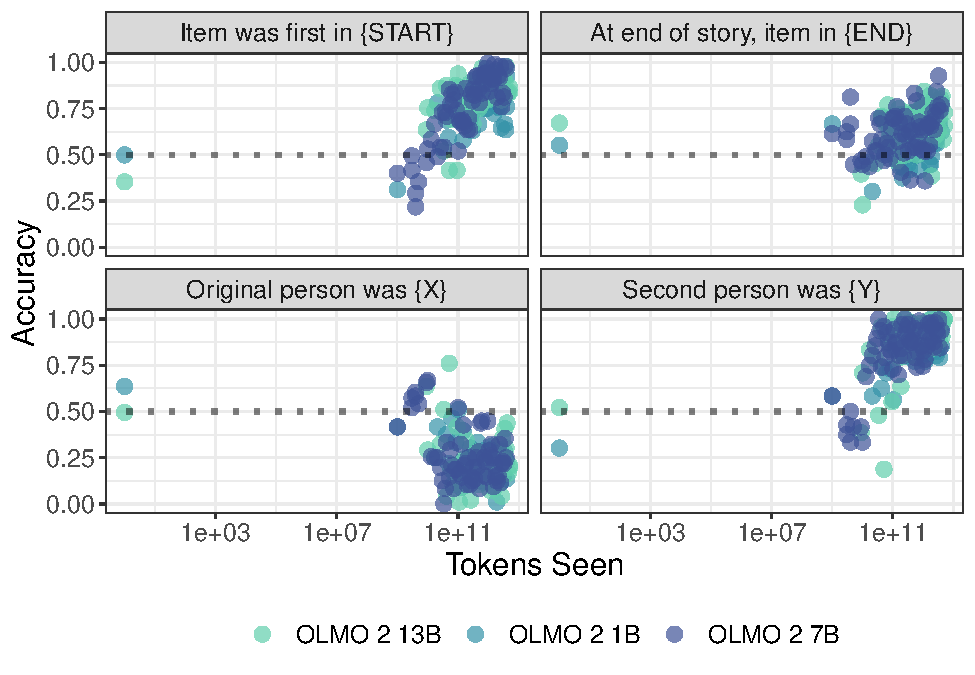
\includegraphics{fb_analysis_files/figure-latex/unnamed-chunk-6-1.pdf}

\begin{Shaded}
\begin{Highlighting}[]
\CommentTok{\# PAPER FIGURE: plot same for the Pythias as well}
\NormalTok{df\_summ }\SpecialCharTok{\%\textgreater{}\%}
  \FunctionTok{filter}\NormalTok{(}\FunctionTok{grepl}\NormalTok{(}\StringTok{"Pythia"}\NormalTok{, model\_shorthand)) }\SpecialCharTok{\%\textgreater{}\%}
  \FunctionTok{ggplot}\NormalTok{(}\FunctionTok{aes}\NormalTok{(}\AttributeTok{x =}\NormalTok{ tokens\_seen\_numeric\_mod,}
             \AttributeTok{y =}\NormalTok{ mean\_accuracy,}
             \AttributeTok{color =}\NormalTok{ model\_shorthand)) }\SpecialCharTok{+}
  \FunctionTok{geom\_point}\NormalTok{(}\AttributeTok{size =} \DecValTok{3}\NormalTok{,}
             \AttributeTok{alpha =}\NormalTok{ .}\DecValTok{7}\NormalTok{) }\SpecialCharTok{+}
  \FunctionTok{geom\_hline}\NormalTok{(}\AttributeTok{yintercept =}\NormalTok{ .}\DecValTok{5}\NormalTok{, }\AttributeTok{linetype =} \StringTok{"dotted"}\NormalTok{,}
             \AttributeTok{size =} \FloatTok{1.2}\NormalTok{, }\AttributeTok{alpha =}\NormalTok{ .}\DecValTok{5}\NormalTok{) }\SpecialCharTok{+}
  \FunctionTok{scale\_x\_log10}\NormalTok{(}\AttributeTok{labels =}\NormalTok{ scales}\SpecialCharTok{::}\FunctionTok{comma\_format}\NormalTok{()) }\SpecialCharTok{+}
  \CommentTok{\# geom\_text\_repel(aes(label=model\_shorthand), size=3) +}
  \FunctionTok{scale\_y\_continuous}\NormalTok{(}\AttributeTok{limits =} \FunctionTok{c}\NormalTok{(}\DecValTok{0}\NormalTok{, }\DecValTok{1}\NormalTok{)) }\SpecialCharTok{+}
  \FunctionTok{labs}\NormalTok{(}\AttributeTok{title =} \StringTok{"Development of Situation Model"}\NormalTok{,}
       \AttributeTok{x =} \StringTok{"Tokens Seen"}\NormalTok{,}
       \AttributeTok{y =} \StringTok{"Accuracy"}\NormalTok{,}
       \AttributeTok{color =} \StringTok{""}\NormalTok{,}
       \AttributeTok{shape =} \StringTok{""}\NormalTok{) }\SpecialCharTok{+}
  \FunctionTok{theme\_bw}\NormalTok{() }\SpecialCharTok{+}
  \FunctionTok{scale\_color\_manual}\NormalTok{(}\AttributeTok{values =}\NormalTok{ viridisLite}\SpecialCharTok{::}\FunctionTok{viridis}\NormalTok{(}\DecValTok{4}\NormalTok{, }\AttributeTok{option =} \StringTok{"mako"}\NormalTok{, }
                                                  \AttributeTok{begin =} \FloatTok{0.8}\NormalTok{, }\AttributeTok{end =} \FloatTok{0.15}\NormalTok{)) }\SpecialCharTok{+}
  \FunctionTok{theme}\NormalTok{(}\AttributeTok{text =} \FunctionTok{element\_text}\NormalTok{(}\AttributeTok{size =} \DecValTok{15}\NormalTok{),}
        \AttributeTok{legend.position=}\StringTok{"bottom"}\NormalTok{) }\SpecialCharTok{+}
  \FunctionTok{facet\_wrap}\NormalTok{(}\SpecialCharTok{\textasciitilde{}}\FunctionTok{reorder}\NormalTok{(q\_label, question\_id))}
\end{Highlighting}
\end{Shaded}

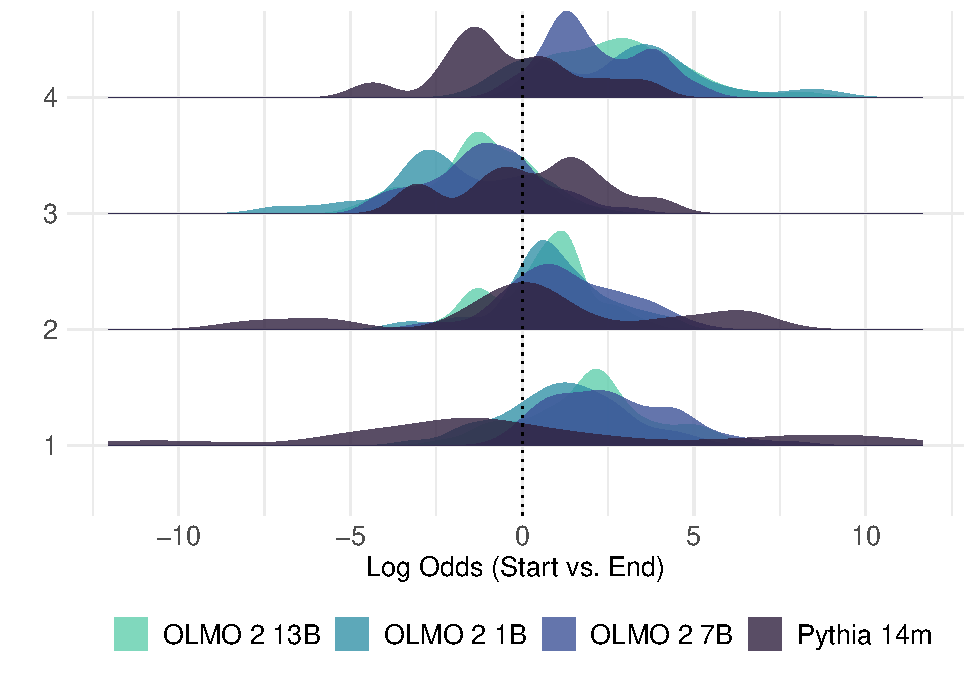
\includegraphics{fb_analysis_files/figure-latex/unnamed-chunk-6-2.pdf}

\begin{Shaded}
\begin{Highlighting}[]
\DocumentationTok{\#\#\# Final step}
\NormalTok{df\_model\_max }\OtherTok{=}\NormalTok{ df\_attn\_check }\SpecialCharTok{\%\textgreater{}\%}
  \FunctionTok{group\_by}\NormalTok{(model\_shorthand) }\SpecialCharTok{\%\textgreater{}\%}
  \FunctionTok{summarise}\NormalTok{(}\AttributeTok{max\_step =} \FunctionTok{max}\NormalTok{(step, }\AttributeTok{na.rm =} \ConstantTok{TRUE}\NormalTok{))}

\NormalTok{df\_attn\_check }\SpecialCharTok{\%\textgreater{}\%} 
  \FunctionTok{inner\_join}\NormalTok{(df\_model\_max) }\SpecialCharTok{\%\textgreater{}\%}
  \FunctionTok{filter}\NormalTok{(step }\SpecialCharTok{==}\NormalTok{ max\_step) }\SpecialCharTok{\%\textgreater{}\%}
  \FunctionTok{ggplot}\NormalTok{(}\FunctionTok{aes}\NormalTok{(}\AttributeTok{x =}\NormalTok{ log\_odds,}
             \AttributeTok{y =} \FunctionTok{factor}\NormalTok{(question\_id),}
             \AttributeTok{fill =}\NormalTok{ model\_shorthand)) }\SpecialCharTok{+}
  \FunctionTok{geom\_density\_ridges2}\NormalTok{(}\FunctionTok{aes}\NormalTok{(}\AttributeTok{height =}\NormalTok{ ..density..), }
                       \AttributeTok{color=}\ConstantTok{NA}\NormalTok{, }
                       \AttributeTok{scale=}\NormalTok{.}\DecValTok{85}\NormalTok{, }
                       \CommentTok{\# size=1, }
                       \AttributeTok{alpha =}\NormalTok{ .}\DecValTok{6}\NormalTok{,}
                       \AttributeTok{stat=}\StringTok{"density"}\NormalTok{) }\SpecialCharTok{+}
  \FunctionTok{labs}\NormalTok{(}\AttributeTok{x =} \StringTok{"Log Odds (Start vs. End)"}\NormalTok{,}
       \AttributeTok{y =} \StringTok{""}\NormalTok{,}
       \AttributeTok{fill =} \StringTok{""}\NormalTok{) }\SpecialCharTok{+}
  \FunctionTok{theme\_minimal}\NormalTok{() }\SpecialCharTok{+}
  \FunctionTok{geom\_vline}\NormalTok{(}\AttributeTok{xintercept =} \DecValTok{0}\NormalTok{, }\AttributeTok{linetype =} \StringTok{"dotted"}\NormalTok{) }\SpecialCharTok{+}
  \FunctionTok{theme}\NormalTok{(}
    \AttributeTok{legend.position =} \StringTok{"bottom"}
\NormalTok{  ) }\SpecialCharTok{+} 
  \FunctionTok{theme}\NormalTok{(}\AttributeTok{axis.title =} \FunctionTok{element\_text}\NormalTok{(}\AttributeTok{size=}\FunctionTok{rel}\NormalTok{(}\FloatTok{1.2}\NormalTok{)),}
        \AttributeTok{axis.text =} \FunctionTok{element\_text}\NormalTok{(}\AttributeTok{size =} \FunctionTok{rel}\NormalTok{(}\FloatTok{1.2}\NormalTok{)),}
        \AttributeTok{legend.text =} \FunctionTok{element\_text}\NormalTok{(}\AttributeTok{size =} \FunctionTok{rel}\NormalTok{(}\FloatTok{1.2}\NormalTok{)),}
        \AttributeTok{legend.title =} \FunctionTok{element\_text}\NormalTok{(}\AttributeTok{size =} \FunctionTok{rel}\NormalTok{(}\FloatTok{1.2}\NormalTok{)),}
        \AttributeTok{strip.text.x =} \FunctionTok{element\_text}\NormalTok{(}\AttributeTok{size =} \FunctionTok{rel}\NormalTok{(}\FloatTok{1.2}\NormalTok{))) }\SpecialCharTok{+}
    \FunctionTok{scale\_fill\_manual}\NormalTok{(}\AttributeTok{values =}\NormalTok{ viridisLite}\SpecialCharTok{::}\FunctionTok{viridis}\NormalTok{(}\DecValTok{7}\NormalTok{, }\AttributeTok{option =} \StringTok{"mako"}\NormalTok{, }
                                                    \AttributeTok{begin =} \FloatTok{0.8}\NormalTok{, }\AttributeTok{end =} \FloatTok{0.15}\NormalTok{)) }
\end{Highlighting}
\end{Shaded}

\begin{verbatim}
## Joining with `by = join_by(model_shorthand)`
\end{verbatim}

\begin{verbatim}
## Warning: The dot-dot notation (`..density..`) was deprecated in ggplot2 3.4.0.
## i Please use `after_stat(density)` instead.
## This warning is displayed once every 8 hours.
## Call `lifecycle::last_lifecycle_warnings()` to see where this warning was
## generated.
\end{verbatim}

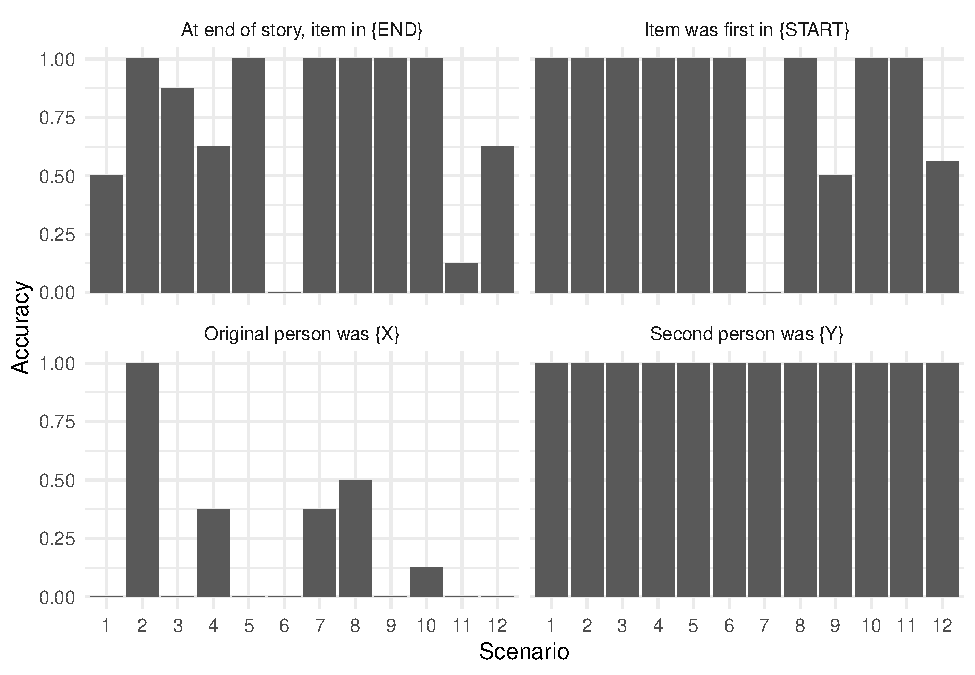
\includegraphics{fb_analysis_files/figure-latex/unnamed-chunk-6-3.pdf}

\begin{Shaded}
\begin{Highlighting}[]
\CommentTok{\#df\_olmo13\_attn\_check \%\textgreater{}\% }
\CommentTok{\#  inner\_join(df\_model\_max) \%\textgreater{}\%}
\CommentTok{\#  filter(step == max\_step) \%\textgreater{}\%}
\CommentTok{\#  group\_by(model\_shorthand, question\_id) \%\textgreater{}\%}
\CommentTok{\#  summarise(mean\_accuracy = mean(correct),}
\CommentTok{\#            step = mean(step))}



\CommentTok{\#df\_items = df\_olmo13\_attn\_check \%\textgreater{}\% }
 \CommentTok{\# inner\_join(df\_model\_max) \%\textgreater{}\%}
 \CommentTok{\# filter(step == max\_step) \%\textgreater{}\%}
 \CommentTok{\# group\_by(model\_shorthand, item, question\_id, q\_label,}
 \CommentTok{\#          correct\_answer, distractor\_answer) \%\textgreater{}\%}
 \CommentTok{\# summarise(mean\_accuracy = mean(correct))}


\CommentTok{\#df\_items \%\textgreater{}\%}
\CommentTok{\#  filter(model\_shorthand == "OLMO 2 13B") \%\textgreater{}\%}
\CommentTok{\#  ggplot(aes(x = factor(item),}
 \CommentTok{\#            y = mean\_accuracy)) +}
 \DocumentationTok{\#\# geom\_bar(stat = "identity") +}
\CommentTok{\#  facet\_wrap(\textasciitilde{}q\_label) +}
\CommentTok{\#  labs(x = "Scenario",}
 \CommentTok{\#      y = "Accuracy") +}
 \CommentTok{\# theme\_minimal()}
\end{Highlighting}
\end{Shaded}


\end{document}
